\documentclass{Libs/report}
\usepackage{float}
\usepackage{graphicx}
\usepackage[
backend=biber,
style=numeric
]{biblatex}
\usepackage{csquotes}
\usepackage{alertmessage}
%\usepackage{soul}
%\usepackage{showframe}

\usepackage[dvipsnames]{xcolor}
\usepackage{sectsty}
\sectionfont{\color{red!80}}  % sets colour of chapters
\subsectionfont{\color{BrickRed}}  % sets colour of sections
\subsubsectionfont{\color{BrickRed!50}}  % sets colour of sections
\paragraphfont{\color{gray!80}}  % sets colour of sections


\usepackage[x11names]{xcolor}
\usepackage{tikz}
% from https://tex.stackexchange.com/a/167024/121799
\newcommand{\ColorList}{red,DarkOrange1,Goldenrod1,Green3,blue!50!cyan,DarkOrchid2,Apricot,Blue,Brown,Aquamarine,BlueGreen,BurntOrange,Bittersweet,BlueViolet,CadetBlue,Black,BrickRed,CarnationPink,Cerulean,CornflowerBlue,Cyan,Dandelion,DarkOrchid,Emerald,ForestGreen,Fuchsia,Goldenrod,Gray,Green,GreenYellow,JungleGreen,Lavender,LimeGreen,Magenta,Mahogany,Maroon,Melon,MidnightBlue,Mulberry,NavyBlue,OliveGreen,Orange,OrangeRed,Orchid,Peach,Periwinkle,PineGreen,Plum,ProcessBlue,Purple,RawSienna,Red,RedOrange,RedViolet,Rhodamine,RoyalBlue,RoyalPurple,RubineRed,Salmon,SeaGreen,Sepia,SkyBlue,SpringGreen,Tan,TealBlue,Thistle,Turquoise,Violet,VioletRed,White,WildStrawberry,Yellow,YellowGreen,YellowOrange}

% Enum lists
\newcommand{\ColoredListItemI}[1]{\foreach \X[count=\Y] in \ColorList
{\ifnum\Y=#1\relax
\xdef\ItemColorI{\X}
\fi
}

\tikz[baseline=(ColoredListItemI.base),remember picture]{%
\node[fill=\ItemColorI,inner sep=4pt,font=\sffamily,fill opacity=0.5] (ColoredListItemI){#1};}
}

% Enum lists nested
\newcommand{\ColoredListItemII}[1]{

\xdef\ItemColorIII{Gray}

\tikz[baseline=(ColoredListItemII.base),remember picture]{%
\node[circle,fill=\ItemColorII,inner sep=2.25pt,font=\sffamily,fill opacity=0.5] (ColoredListItemII){#1};}
}

% Item lists
\newcommand{\ColoredListItemIII}[1]{

\xdef\ItemColorIII{ForestGreen}

\tikz[baseline=(ColoredListItemIII.base),remember picture]{%
\node[circle,fill=\ItemColorIII,inner sep=2.25pt,font=\sffamily,fill opacity=0.5] (ColoredListItemIII){.};}
}

% My box
\newcommand{\mybox}[1]{\colorbox{OliveGreen!50}{\textcolor{white}{\textit{``#1''}}}}

% \usepackage{luacolor,lua-ul} %for usage of style attributes - background color

% \newcommand{\mybox}[1]{\highLight[{OliveGreen!50}]{#1}}

%\usepackage[skins]{tcolorbox}

%\tcbset{commonstyle/.style={boxrule=0pt,sharp corners,enhanced jigsaw}}

%\newtcolorbox{mycolorbox}[1][]{commonstyle,#1}

%\newcommand{\mybox}[1]{
%\begin{mycolorbox}[colback=OliveGreen!50,drop lifted shadow]
%	#1
%\end{mycolorbox}
%}

% \node[circle,draw=black, fill=white, inner sep=0pt,minimum size=5pt] (b) at (2/3,5/3) {};

% \newcommand{\ColorHighlight}{\tikz[overlay,remember picture]{%
% \fill[\ItemColor,fill opacity=0.5] ([yshift=4pt,xshift=-\pgflinewidth]ColoredListItemI.east) -- ++(4pt,-4pt)
% -- ++(-4pt,-4pt) -- cycle;
% }}

\title{ISTQB Résumé - MBO}
\addbibresource{Libs/bibliography.bib}

\renewcommand{\labelenumii}{\theenumii}
\renewcommand{\theenumii}{\theenumi.\arabic{enumii}.}

\begin{document}

\renewcommand{\labelenumi}{\ColoredListItemI{\arabic{enumi}}}
\renewcommand{\labelenumii}{\ColoredListItemII{.}}
\renewcommand{\labelitemi}{\ColoredListItemIII{\arabic{enumi}}}

\logo{logos/ISTQB_tester}
\ttitle{Résumé ISTQB} % Title of the file
% \subject{ISTQB} % Subject name
%\topic{\small La critique est aisée, mais l'art est difficile\\ \footnotesize \textit{Philippe Néricault}} % Topic name
\topic{Test it or discard it!} % Topic name

\participants{
    \studentinfo{MBO}{06101971}{mathieu.bonnet.1971@gmail.com}
} % You can place many participants in this area, and also names of the tutors, but it is recommended to adjust layout accordingly to make it look better. Notice that for tutor the second position is department, and for students and collaborators it's student ID.
        
\buildmargins % display margins
\buildcover % create the front cover of the document
\toc % creates the table of contents

%------------ Report body ----------------

        % \alertinfo{alertinfo}
        % \alertsuccess{alertsuccess}
        % \alertwarning{alertwarning}
        % \alerterror{alerterror}

%------------ Report body ----------------

\pagebreak

	\begin{center}
        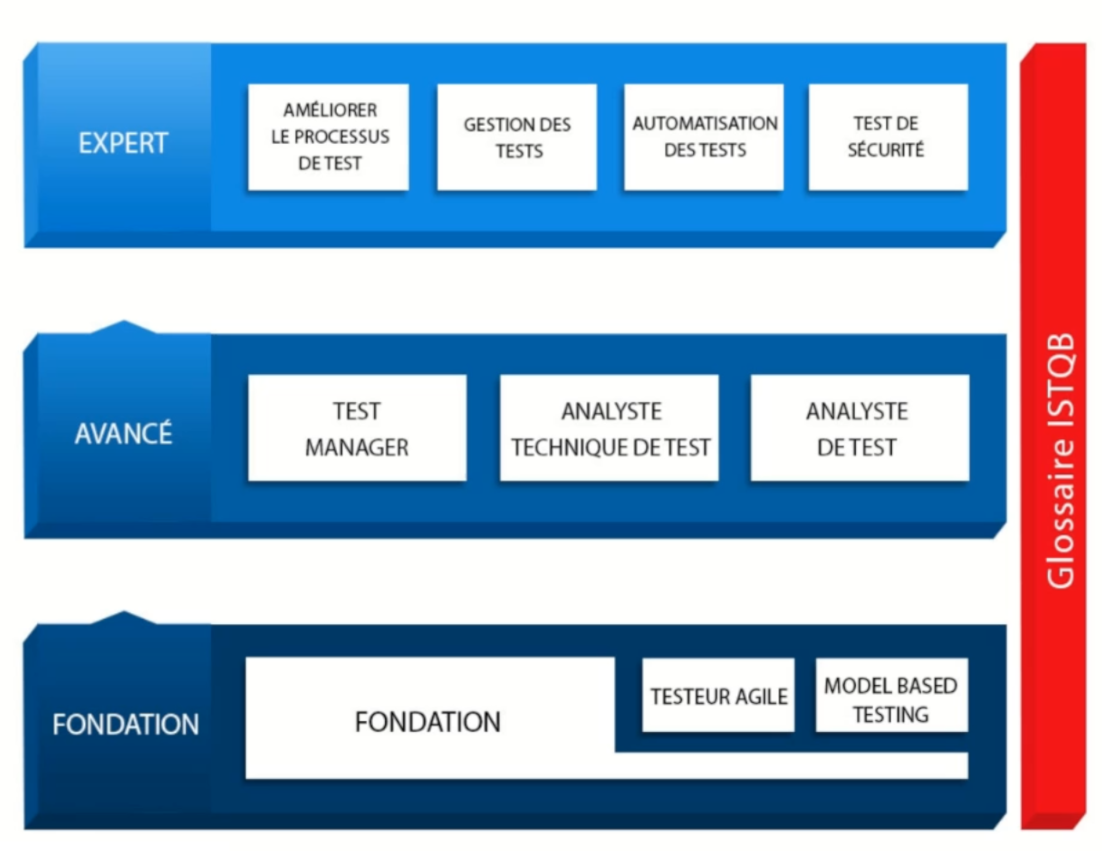
\includegraphics[width=0.9\textwidth]{images/ISTQB_all.png}
    \end{center}
    
\section{LES FONDAMENTAUX DU TEST}

	\subsection{Pourquoi tester}
        Tester pour:
        \begin{itemize}
            \item Limiter le risque de défaillances
            \item Détecter et prévenir les défauts
            \item Assurer la conformité par rapport à des exigences ou à des besoins
            \item Donner de l'information
            \item Gagner de la confiance dans le produit et de la crédibilité auprès du client
            \item ...
        \end{itemize}

        \alertinfo{
        \textbf{Test} $\xrightarrow{}$ \textit{Détection des bugs}
        }
        \alertinfo{
        \textbf{Débogage} $\xrightarrow{}$ \textit{Reproduction, analyse et correction des bugs}
        }    
        
	\subsection{Test et Assurance Qualité (QA)}

    \begin{center}
        
\includegraphics[width=0.9\textwidth]{images/Test Assurance Qualité.png}
    \end{center}
    
    \vspace{-20mm}
    
    \begin{itemize}
        \item Assurance Qualité $\xrightarrow{}$ Préventif - Centré processus
        \item Contrôle Qualité \ \ $\xrightarrow{}$ Curatif (ou réactif) - Centré produit
    \end{itemize}
    
	\subsection{Erreur, défaut et défaillance}

    \alertinfo{
    \textbf{ERREUR} $\xrightarrow{}$ \textit{Action humaine produisant un résultat incorrect. - ISO 24765
    	\newline \color{Brown}{Cette erreur peut être liée à une incompréhension, à une incompétence...}}}
    \alertinfo{
    \textbf{DÉFAUT} $\xrightarrow{}$ \textit{Une imperfection ou une déficience d'un produit d'activités lorsqu'il ne répond pas à ses exigences ou à ses spécifications. - IEEE 1044
    	\newline \color{Brown}{Ce défaut peut provoquer une défaillance (mais pas toujours).}}}
    \alertinfo{
    \textbf{DÉFAILLANCE} $\xrightarrow{}$ \textit{Événement dans lequel un composant ou un système n'exécute pas une fonction requise dans les limites spécifiées. - ISO 24765
    	\newline \color{Brown}{Lors du système en cours d'exécution on constate quelque chose d'inattendu.}}}

    
	\subsection{Les causes racines}

    \alertinfo{\textbf{CAUSE RACINE} $\xrightarrow{}$ \textit{Une source de défaut telle que si elle est retirée, l'apparition de ce type de défaut est diminuée ou supprimée. - CMMI 
    		\newline \color{Brown}{Raison de l'erreur en amont.}}}
    	
    
    Cela peut produire des effets négatifs tels que:
    
    \begin{itemize}
        \item Le désintéressement des utilisateurs
        \item Des pertes financières
        \item Un risque santé ou d'autres types de risque
        \item ...
    \end{itemize}
    
	\subsection{Les principes du test}

    \paragraph{Les 7 principes}

    \begin{enumerate}
        \item  Les tests montrent la présence de défauts, pas leur absence
        \item  Les tests exhaustifs sont impossibles
        \item  Tester tôt économise du temps et de l'argent
        \item  Le regroupement des défauts
        \item  Le paradoxe du pesticide
        \item  Les tests dépendent du contexte
        \item  L'absence d'erreurs est une illusion
    \end{enumerate}

    \subsection{La gestion des tests}

    \begin{center}
        
\includegraphics[width=0.9\textwidth]{images/Gestion des tests.png}
    \end{center}
    
	\subsubsection{Planification}
	
	\begin{center}
		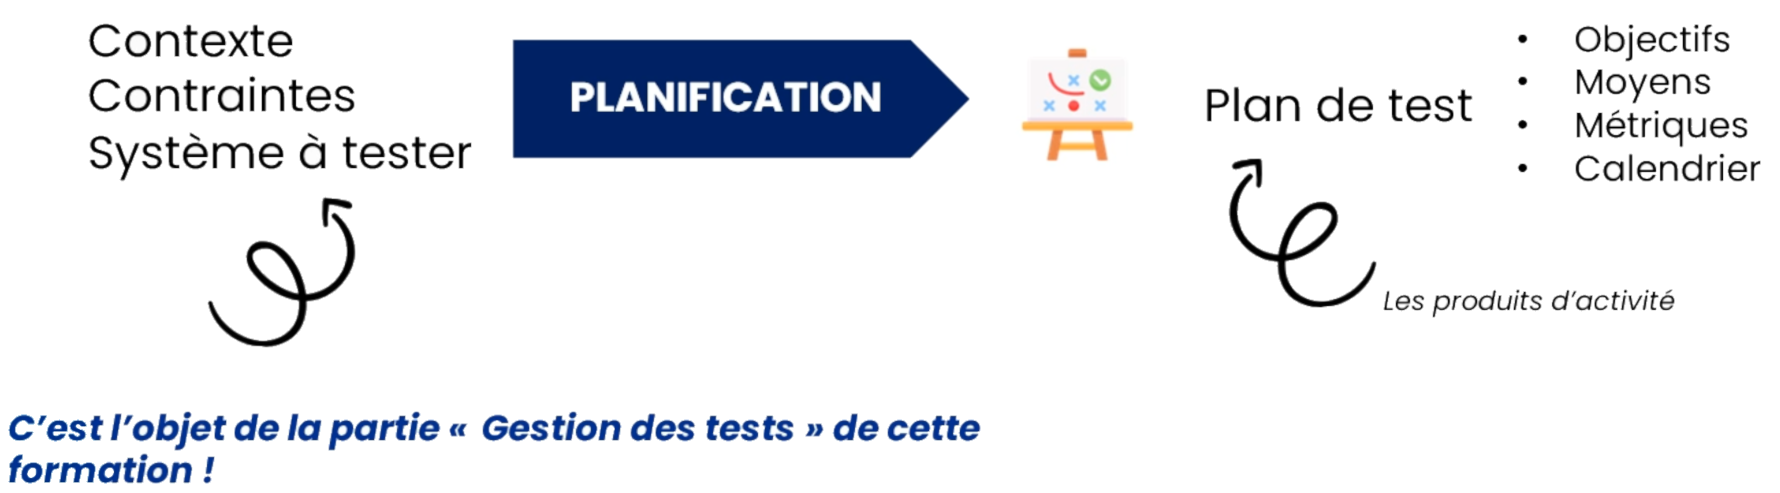
\includegraphics[width=0.9\textwidth]{images/planification.png}
	\end{center}
	
	\paragraph{On produit un document appelé \mybox{Plan de test} contenant:}
	
	 \begin{itemize}
		\item Les objectifs
		\item Le périmètre
		\item Les approches
		\item Les risques
		\item Les parties prenantes et la communication
		\item Les hypothèses et les contraintes
		\item Les moyens
		\item Les métriques
		\item Le calendrier
		\item ...
	\end{itemize}
	
	\alertinfo{\textbf{Plan de test} $\xrightarrow{}$ \textit{Ce document est vivant et évolue tout au long du projet.}}
	
	\begin{center}
		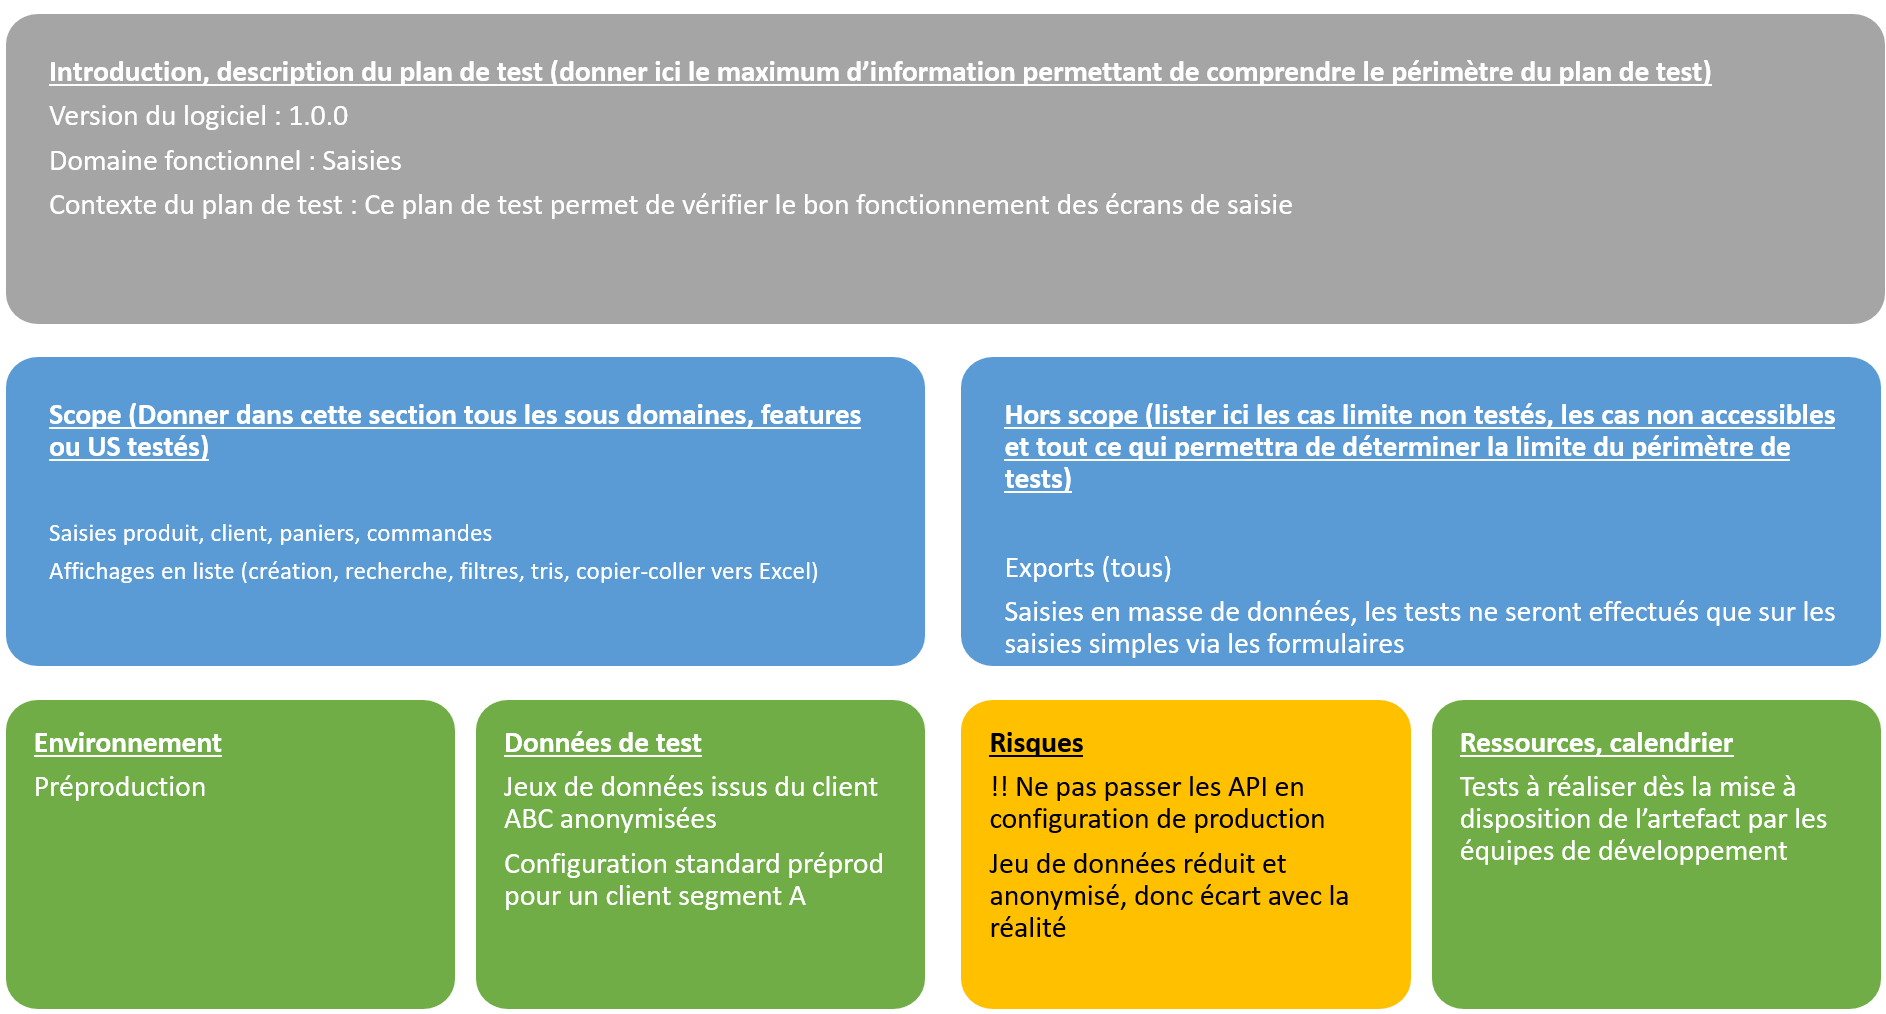
\includegraphics[width=0.9\textwidth]{images/test_plan_01.png}
	\end{center}
	

	\subsubsection{Le suivi et le contrôle (ou le pilotage)}
	
	\paragraph{Le suivi et le contrôle (ou le pilotage) s'effectue tout au long du processus de test. Il produit:}
	
	\begin{itemize}
		\item Les rapports d'avancement
		\item Le rapport de synthèse
		\item Le plan de test revu (n'oublions pas que ce dernier est vivant!)
		\item ...
	\end{itemize}
        

	\subsubsection{L'analyse}

    \begin{center}
        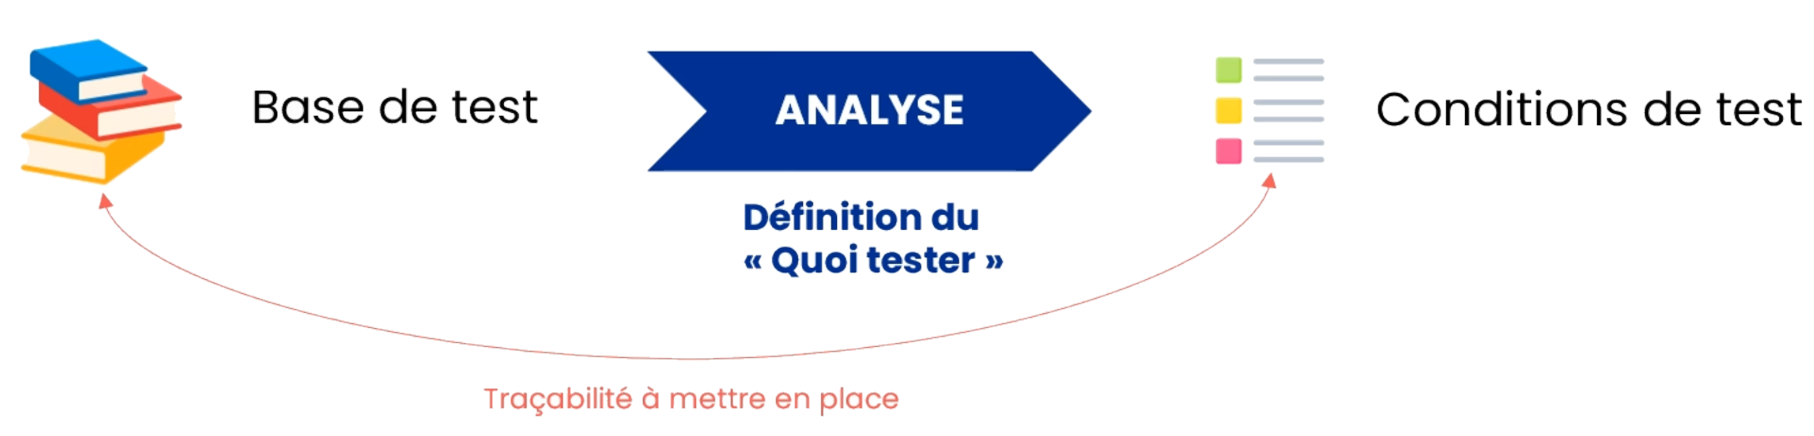
\includegraphics[width=0.9\textwidth]{images/Analyse.png}
    \end{center}

    \paragraph{L'analyse s'appuie sur la \mybox{Base de test} (aussi appelé \mybox{Base des conditions de test}) et produit les \mybox{Conditions de test}.}
    
    \alertinfo{BASE DE TEST\newline L'ensemble des connaissances utilisées comme base pour l'analyse et la conception des tests.}

    \paragraph{Concrètement il faut:}

    \begin{enumerate}
        \item Analyser les bases de test
            \begin{itemize}
                \item Exigences, US, épics, cas d'utilisation, diagrammes, flux d'appels, spécifications fonctionnelles, spécifications techniques, spécifications d'interface, code source de l'application, rapports d'analyse de risque, ...
            \end{itemize}    
        \item Évaluer afin d'identifier les défauts (tester tôt ou shift-left)
            \begin{itemize}
                \item Ambiguïtés, omissions, incohérences, inexactitudes, contradictions, ...
            \end{itemize}
        \item Identifier et prioriser les conditions de test
        \item Assurer une traçabilité bidirectionnelle entre les conditions de test et la base de test
    \end{enumerate}
    
	\subsubsection{La conception}

    \begin{center}
        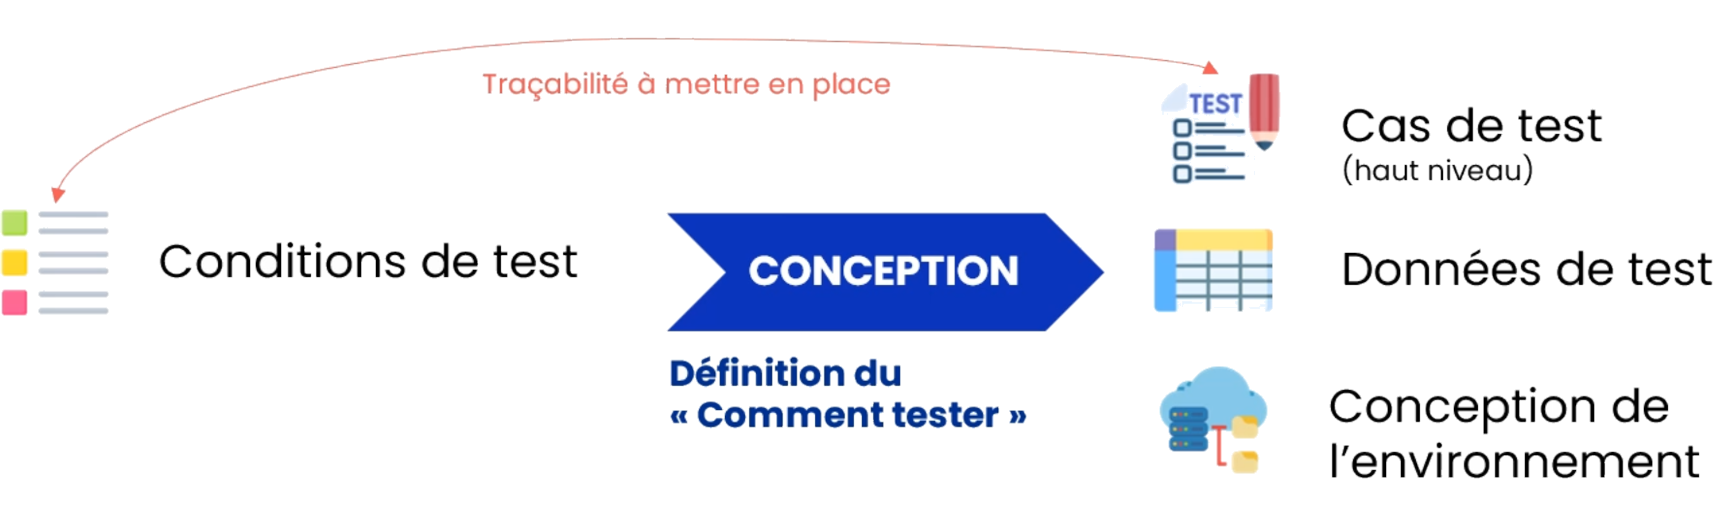
\includegraphics[width=0.9\textwidth]{images/Conception.png}
    \end{center}

    \paragraph{La conception s'appuie sur les \mybox{Conditions de test} et produit les \mybox{Cas de test}, les \mybox{Données de test}, ainsi que l'\mybox{Environnement de test}.}
    
    \alertinfo{CONDITION DE TEST\newline Un aspect des bases de test qui est pertinent pour atteindre des objectifs de	test spécifiques.}
    \alertinfo{CAS DE TEST\newline Un ensemble de conditions préalables, de données d'entrée, d'actions (le cas échéant), de résultats attendus et de postconditions, élaboré sur la base des conditions de test.}
    \alertinfo{DONNÉES DE TEST\newline Données créées ou sélectionnées pour satisfaire les préconditions d'exécution et les entrées pour exécuter un ou plusieurs cas de test.}
    
	\subsubsection{L'implémentation}

    \begin{center}
        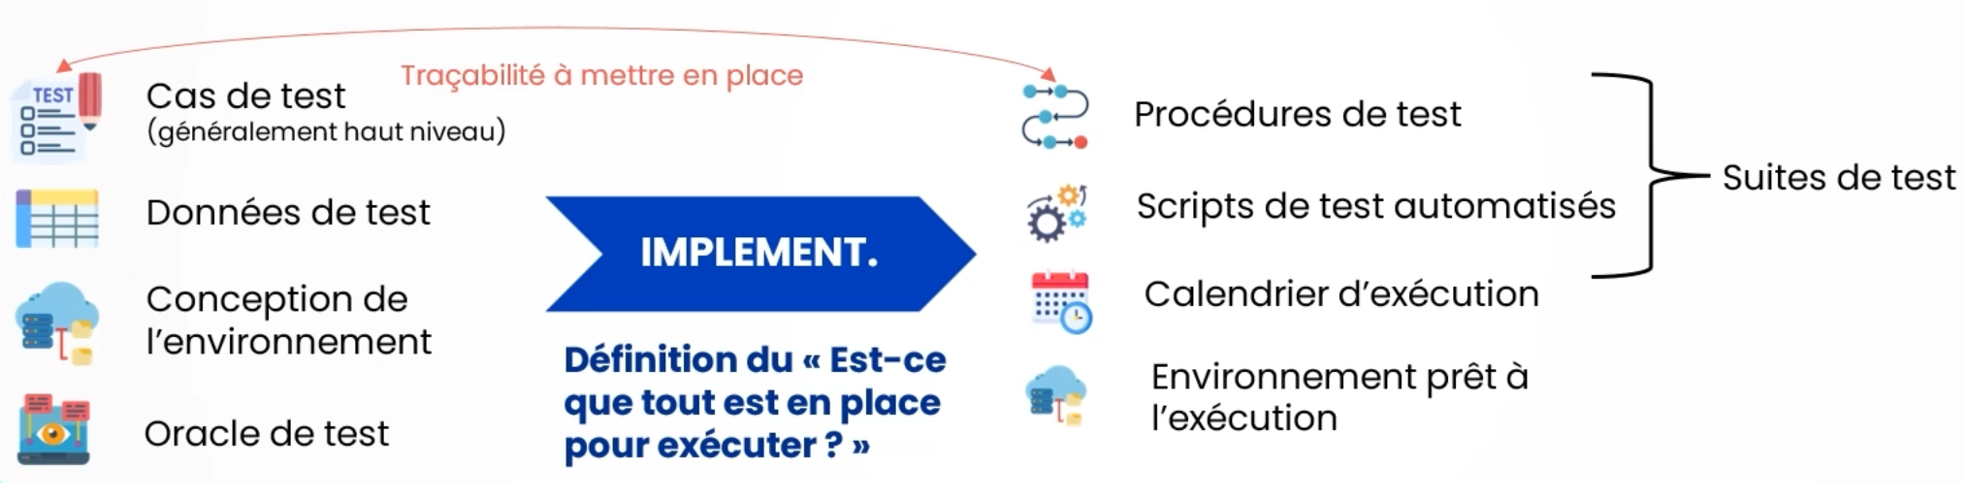
\includegraphics[width=0.9\textwidth]{images/Implémentation.png}
    \end{center}

    \paragraph{L'implémentation s'appuie sur les \mybox{Cas de test}, les \mybox{Données de test} et l'\mybox{Environnement de test} et produit à la fois les \mybox{Procédures de test}, le \mybox{Calendrier d'exécution}, les \mybox{Scripts de test automatisés} et bien évidemment l'\mybox{Environnement prêt à l'execution}.}

    \paragraph{L'ensemble des \mybox{Procédures de test} et des \mybox{Scripts de test automatisé} est appelé \mybox{Suites de test}.}
    
    \alertinfo{PROCÉDURE DE TEST\newline Une séquence de cas de test dans l'ordre d'exécution, et toutes les actions associées qui peuvent être nécessaires pour mettre en place les préconditions initiales et toutes les activités de bouclage après l'exécution.}
    \alertinfo{SUITE DE TEST\newline Ensemble de cas de test ou de procédures de test à exécuter dans un cycle de test spécifique.}
    
	\subsubsection{L'exécution}
	
	\paragraph{L'exécution prend en entrée l'\mybox{oracle de test} et fournit un statut et des rapports.}
	
	\alertinfo{ORACLE DE TEST\newline Source utilisée pour déterminer les résultats attendus à comparer avec les résultats obtenus de l'application en cours de test.}

    \begin{center}
        
\includegraphics[width=0.9\textwidth]{images/Exécution.png}
    \end{center}
    
	\subsubsection{La clôture}

    \begin{center}
        
\includegraphics[width=0.9\textwidth]{images/Clôture.png}
    \end{center}
    
	\subsection{Le processus testware (ou processus de test)}

    \begin{center}
        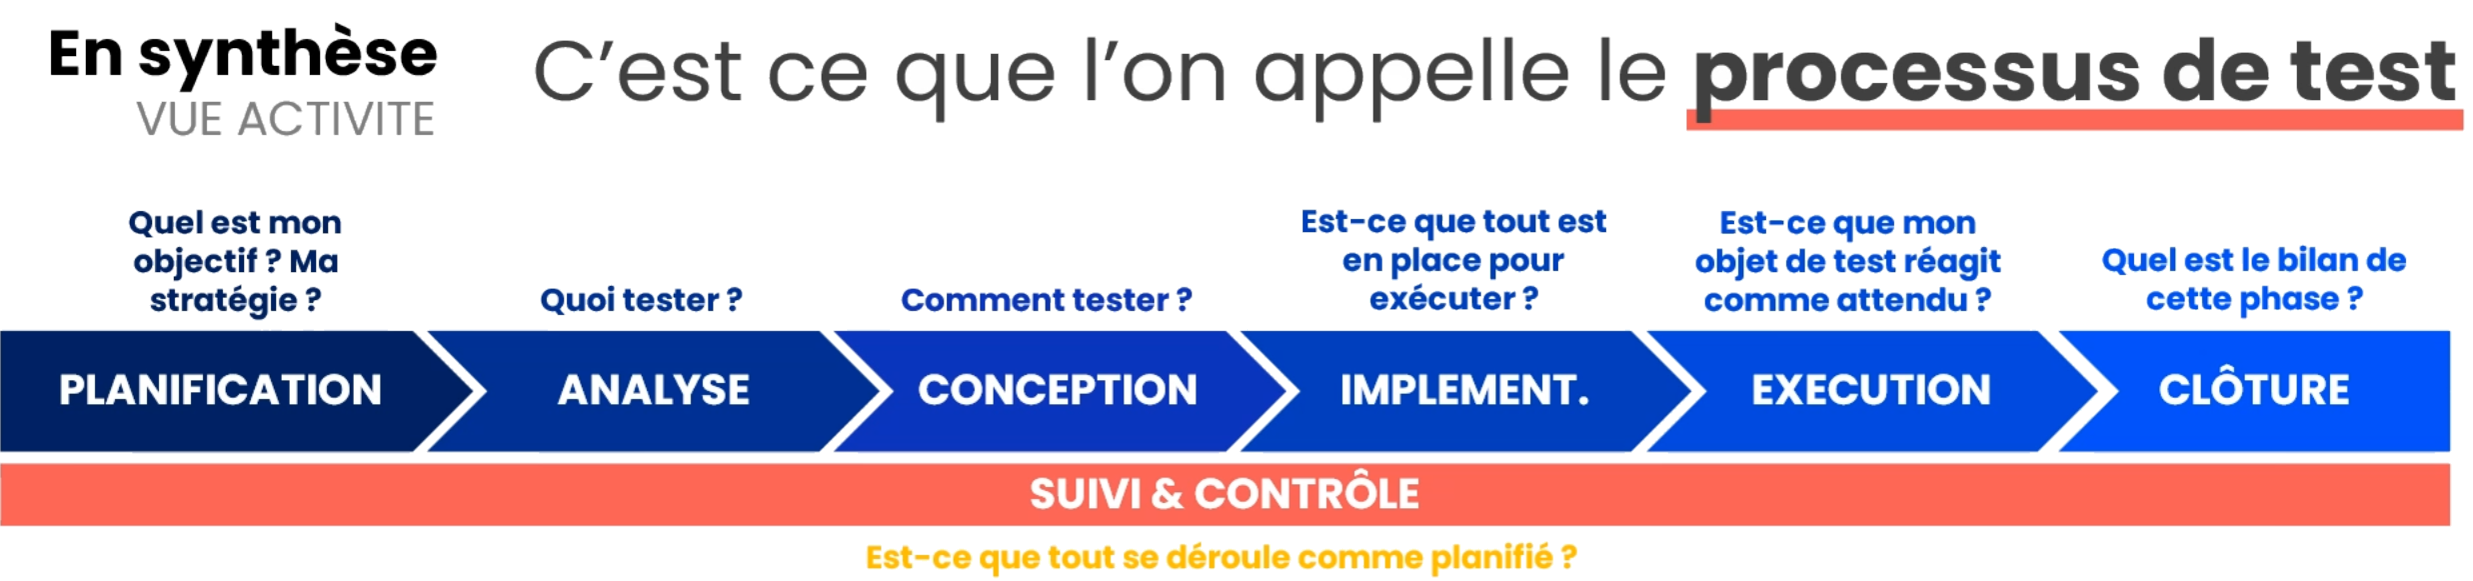
\includegraphics[width=0.9\textwidth]{images/Testware.png}
    \end{center}

    \begin{center}
        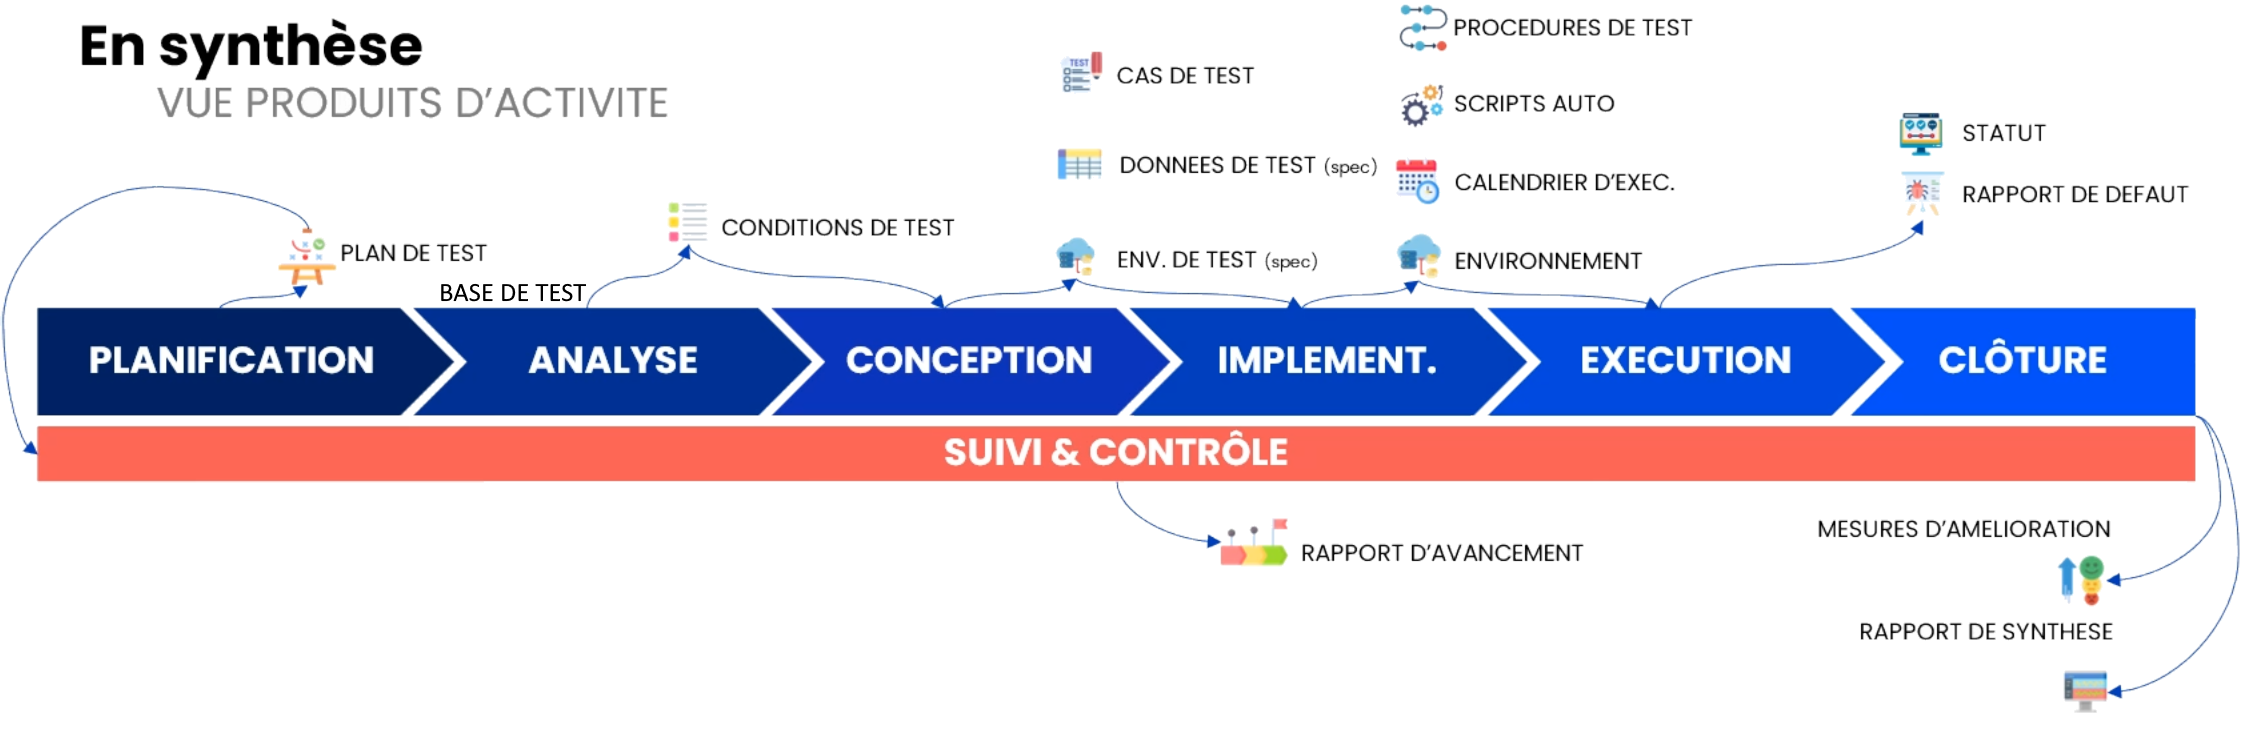
\includegraphics[width=0.9\textwidth]{images/Testware_synthèse.png}
    \end{center}
    
	\subsection{Le processus outillé}

    \begin{center}
        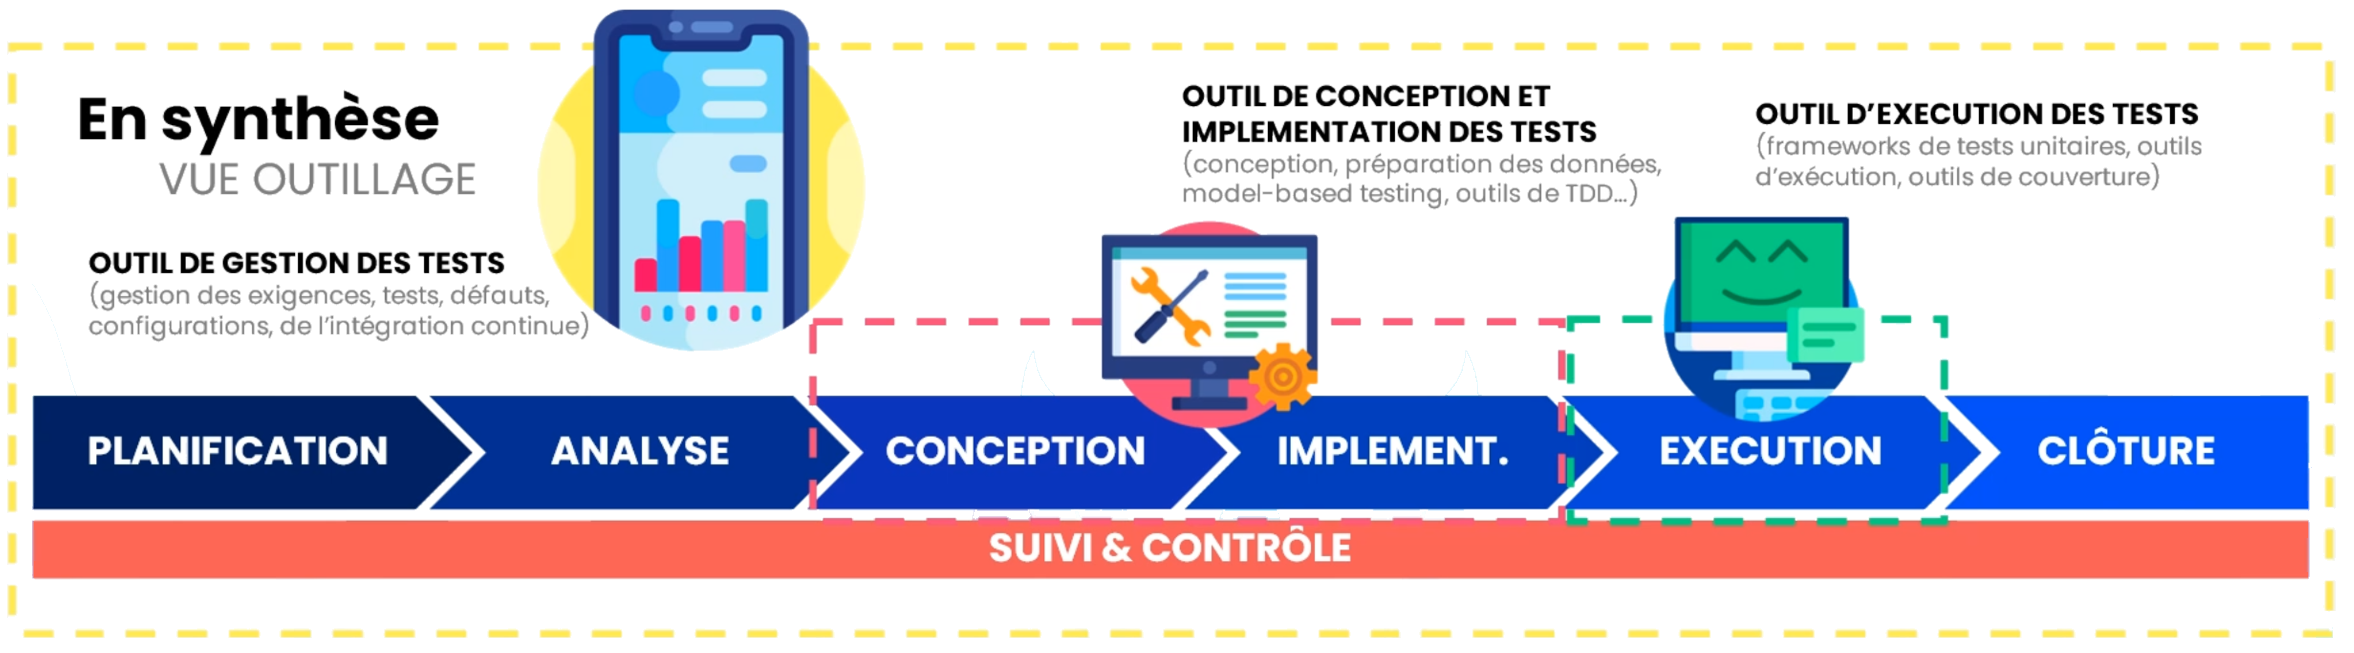
\includegraphics[width=0.9\textwidth]{images/Process_outillé.png}
    \end{center}
    
	\subsection{La traçabilité}
	
	\alertinfo{TRAÇABILITÉ\newline La mesure dans laquelle une relation peut être établie entre deux ou plusieurs produits d'activités.}

    \begin{center}
        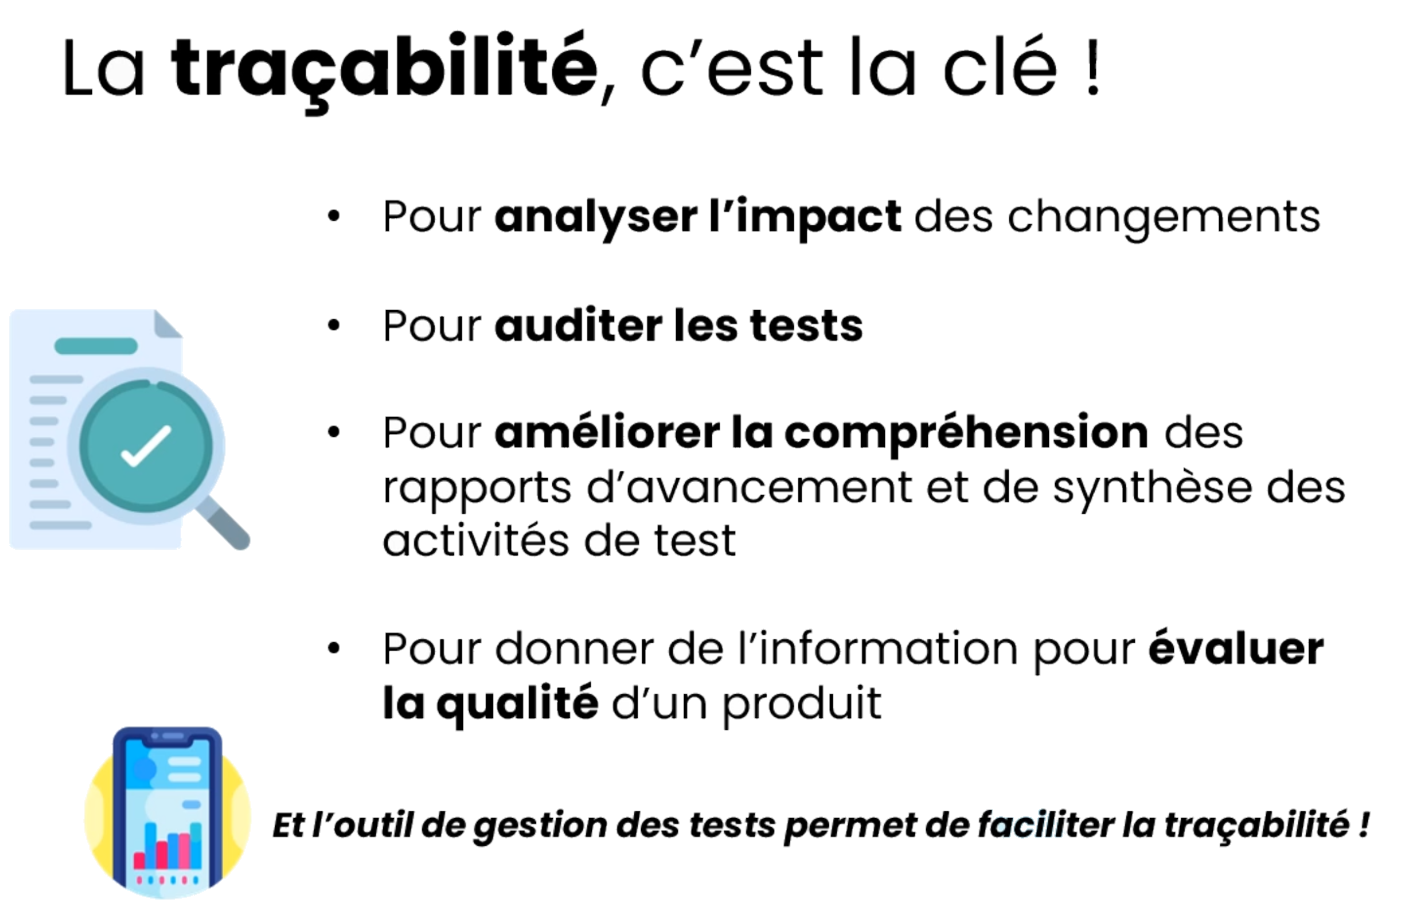
\includegraphics[width=0.9\textwidth]{images/Traçabilité_01.png}
        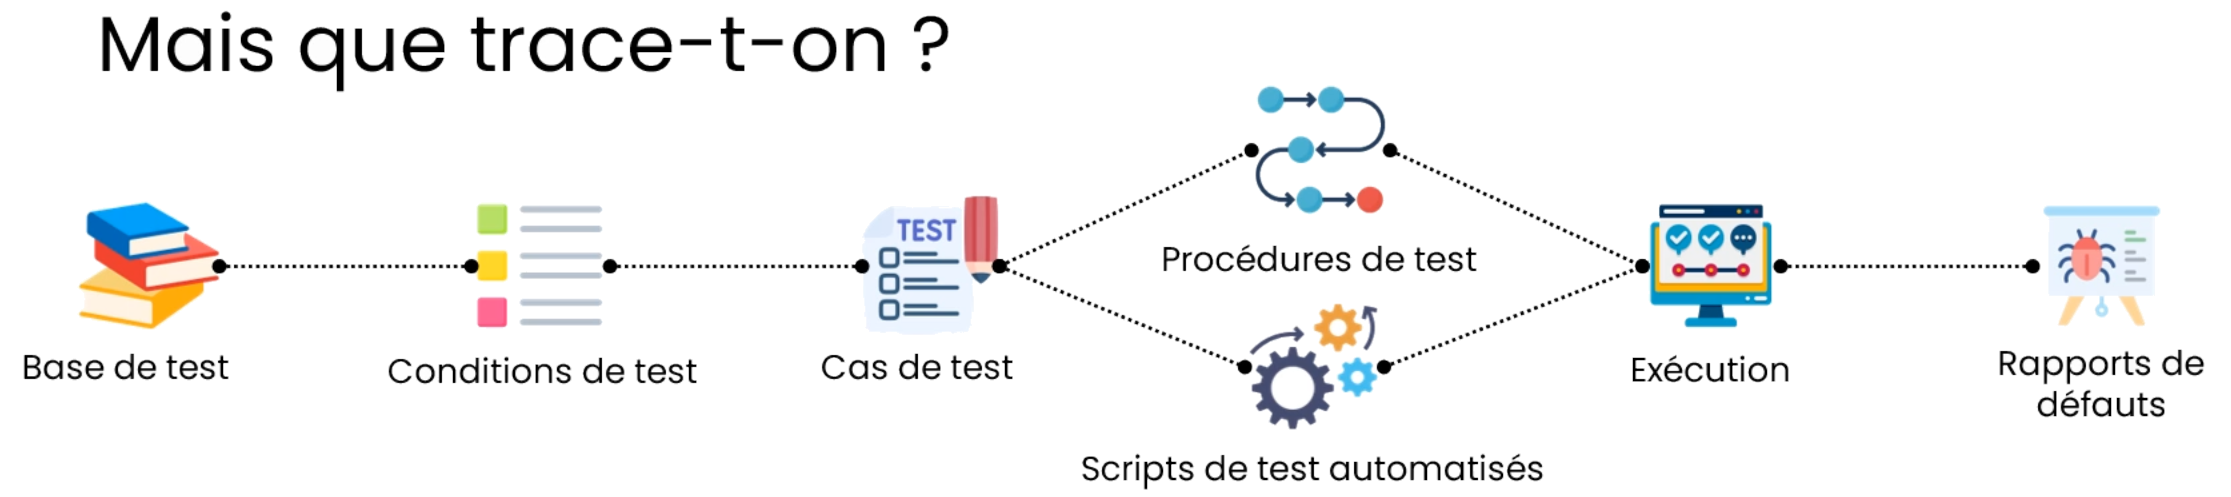
\includegraphics[width=0.9\textwidth]{images/Traçabilité_02.png}
        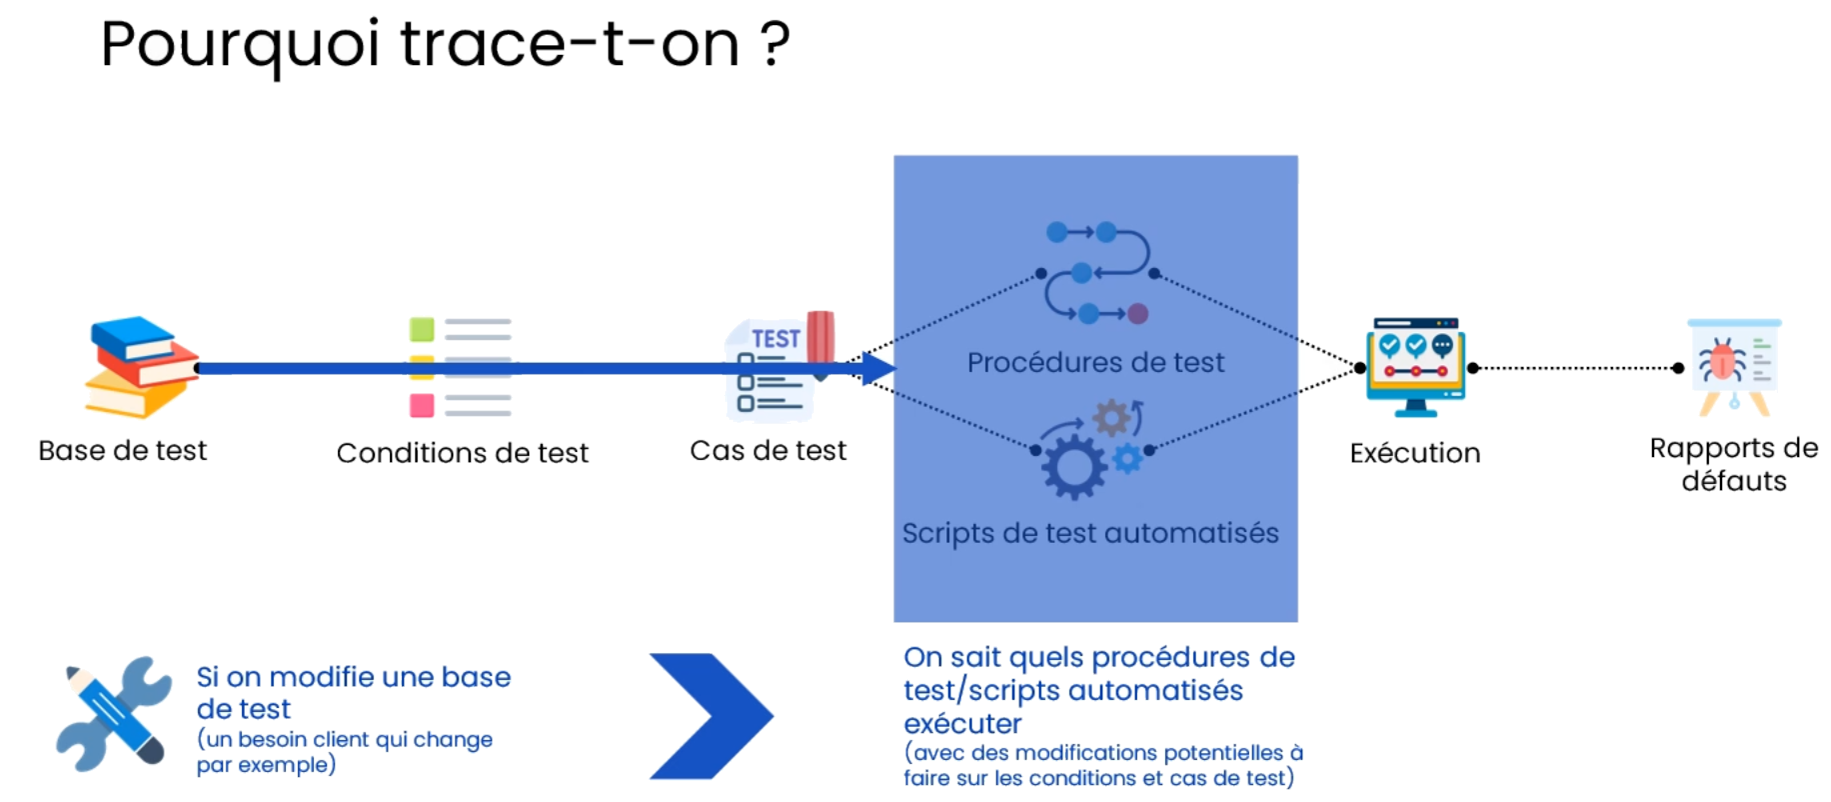
\includegraphics[width=0.9\textwidth]{images/Traçabilité_03.png}
        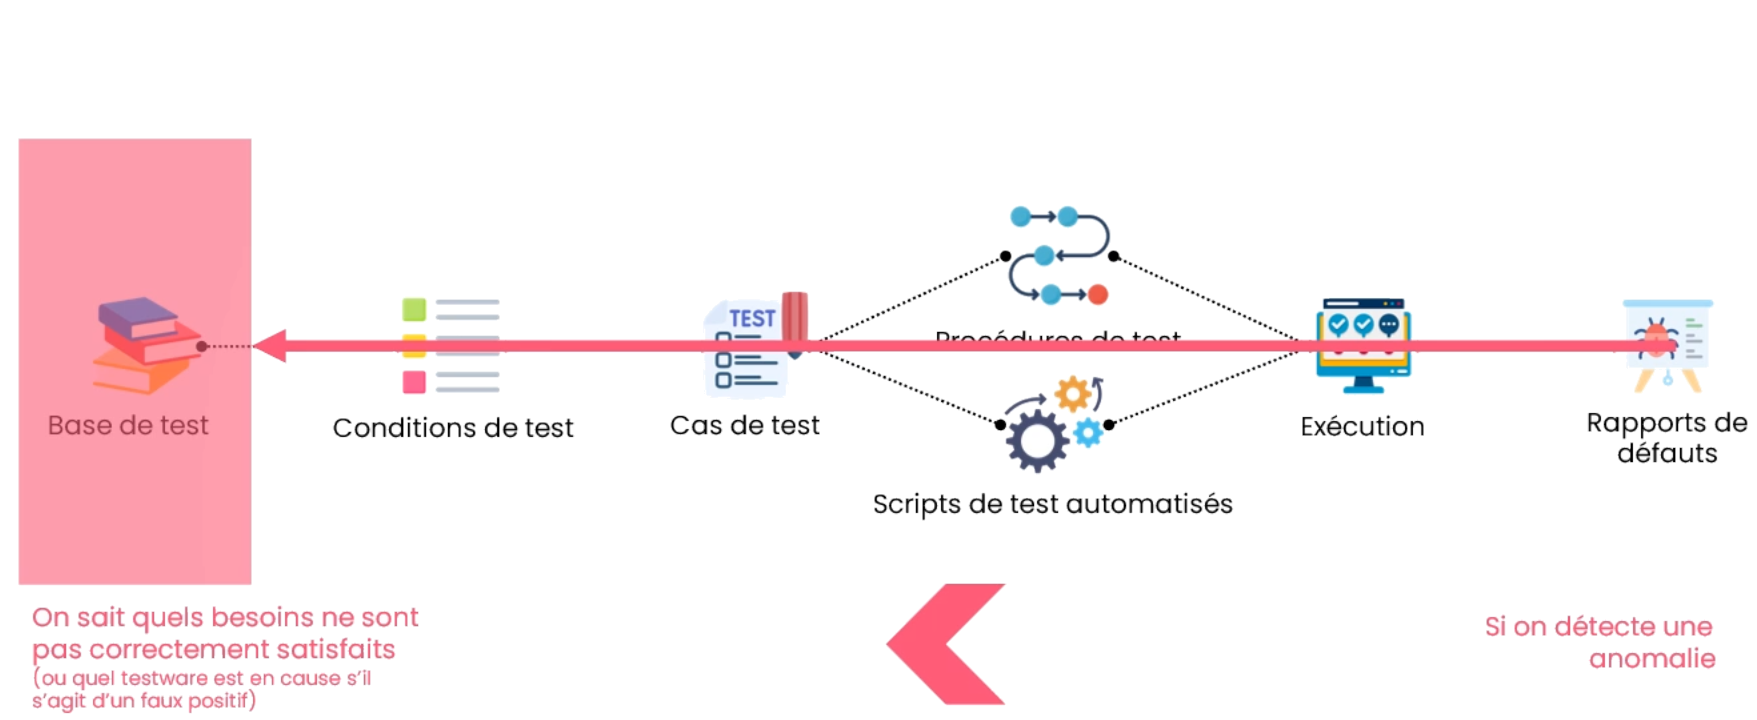
\includegraphics[width=0.9\textwidth]{images/Traçabilité_04.png}
    \end{center}
    
	\subsection{La couverture}

        \begin{center}
        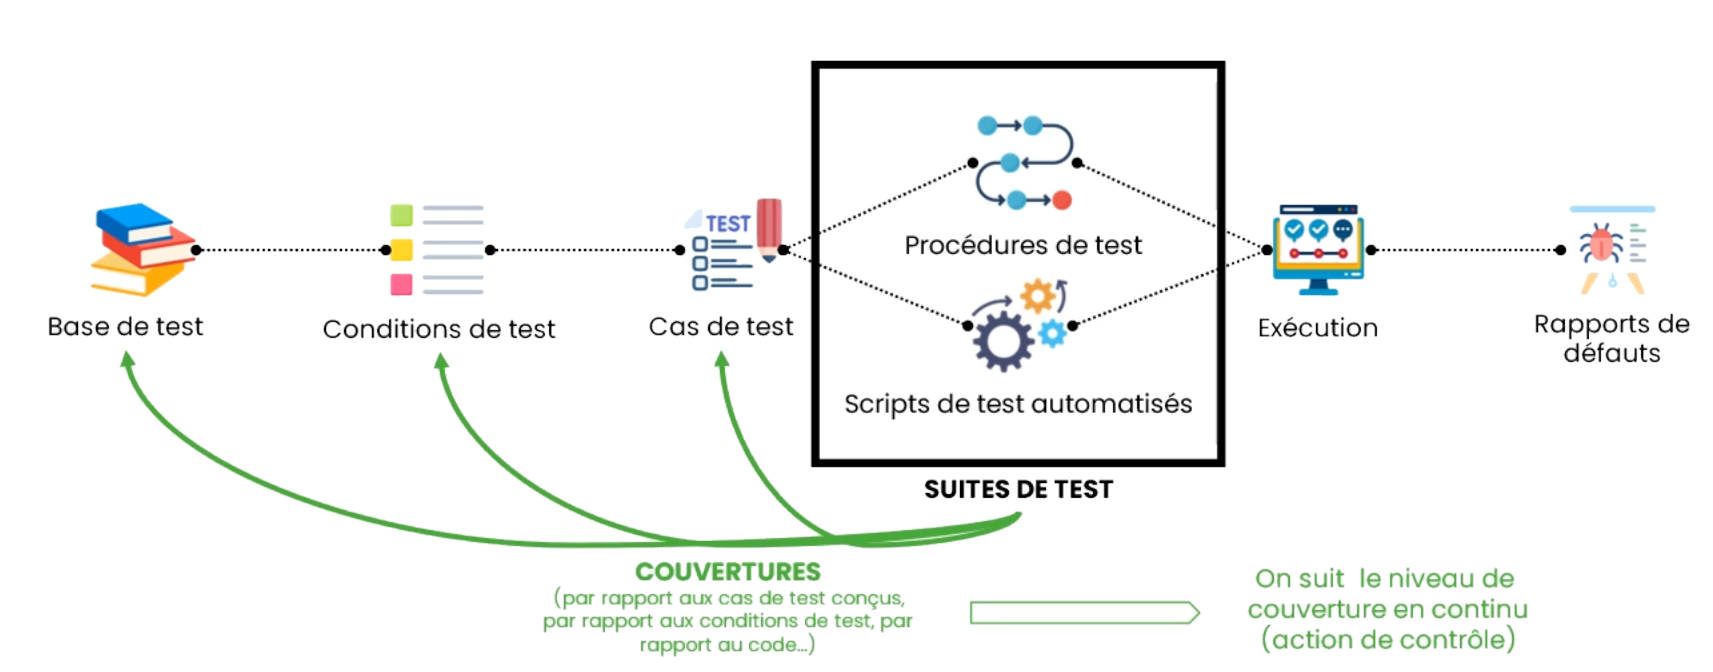
\includegraphics[width=0.9\textwidth]{images/Couverture.png}
    \end{center}
    
    Il existe différents outils dans le métier du test. Un des plus connus et des plus instinctifs est la couverture.\\
    Mais que veut dire exactement j’ai une couverture de 100\% ?\\
    Au risque de vous décevoir : rien ! En effet il existe 3 types de couvertures pour les tests.\\
     Les 3 sont totalement différentes et sont :\\
    
    \subsubsection{La couverture des méthodes (des fonctionnalités)}
    	Cette couverture correspond à la couverture la plus basique. Elle correspond au pourcentage de fonctionnalités avec au moins 1 cas de test effectué.\\
    \subsubsection{La couverture des instructions (du code)}
    	Cette couverture est plus complète que la précédente. Elle correspond au pourcentage de lignes de codes par lesquelles on est passé lors des tests. Plus concrètement on veut que chaque possibilité offerte par l’application soit testée au moins une fois, par contre la façon d’accéder à cette possibilité n’est pas importante.\\
    \subsubsection{La couverture des chemins d’exécution}
    	La couverture la plus complète ! Qui est également une couverture que l’on ne peut généralement pas atteindre ou alors avec un coût particulièrement élevé.\\
    	Ici, en plus de tester toutes les lignes du code on test également tous les moyens d’y arriver, tous les chemins possible.\\
    
	\subsection{Les rôles et l'état d'esprit}

    \begin{center}
        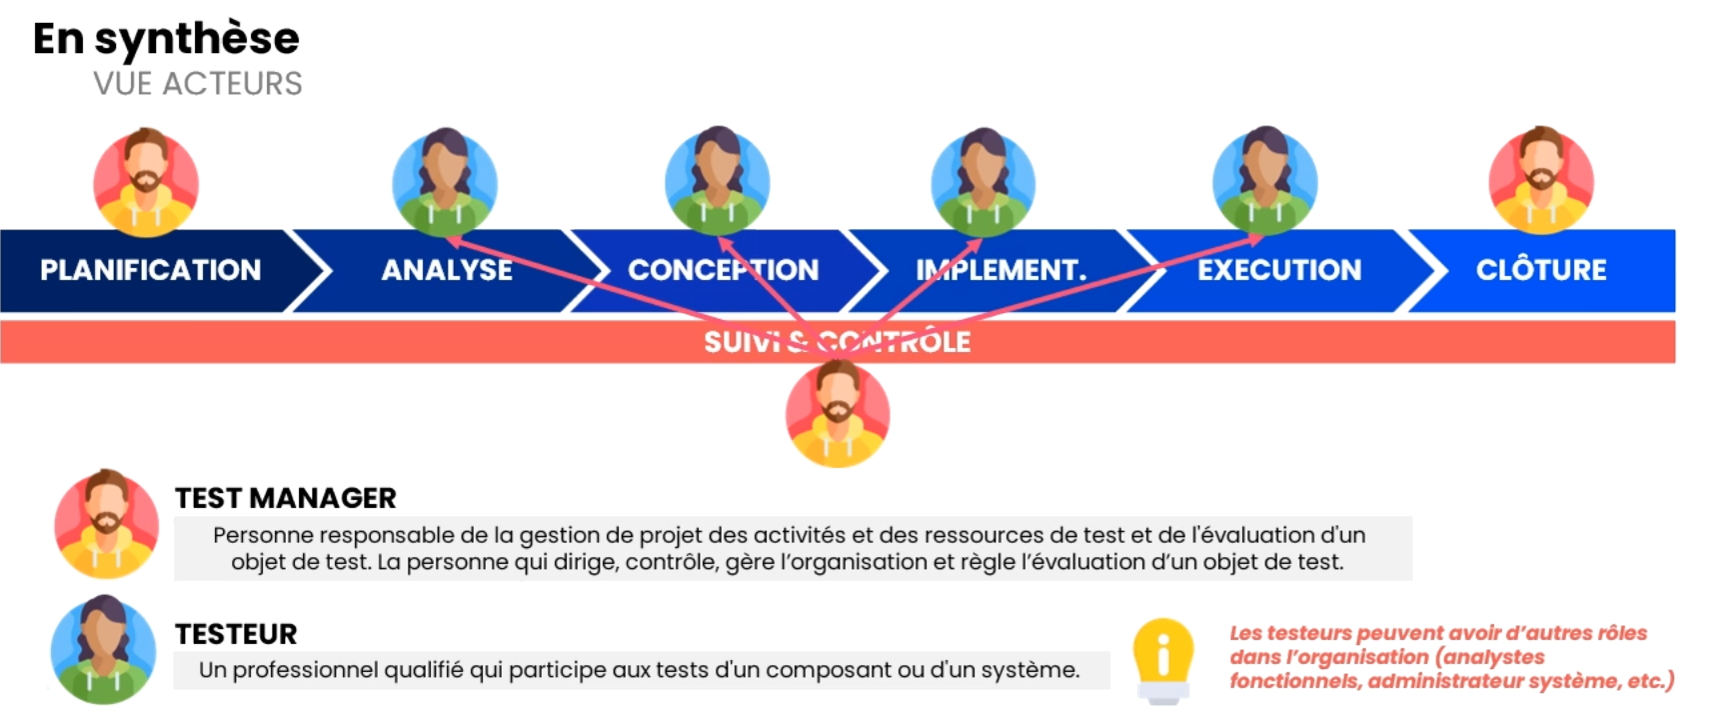
\includegraphics[width=0.9\textwidth]{images/Rôles_01.png}
        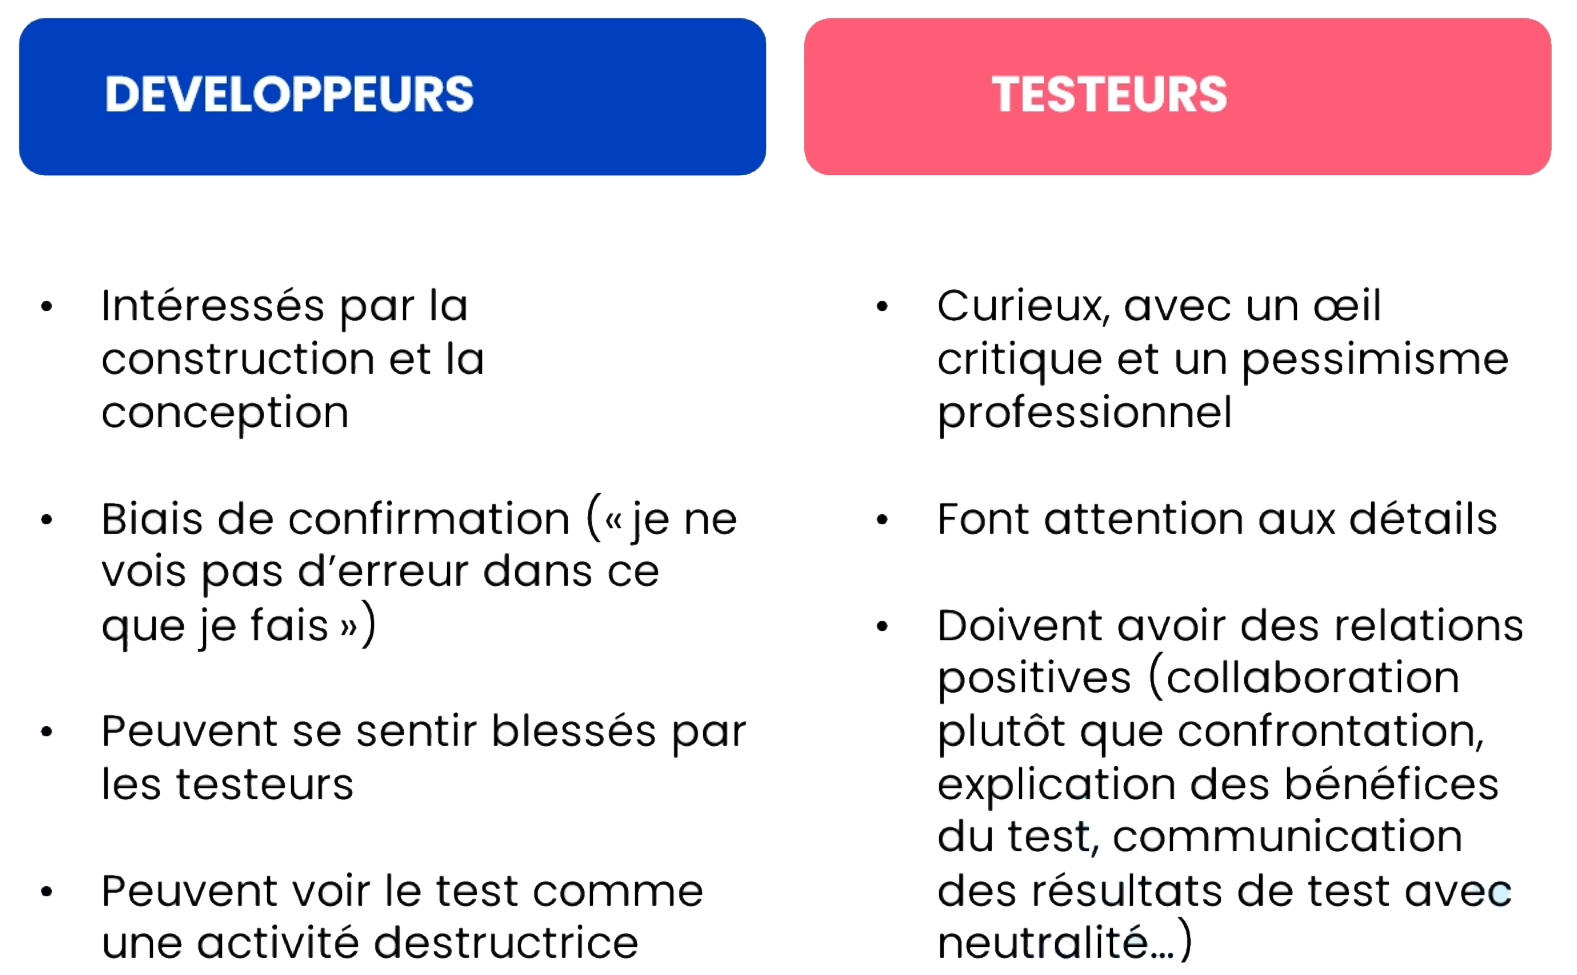
\includegraphics[width=0.9\textwidth]{images/Rôles_02.png}
    \end{center}
    
	\subsection{L'indépendance des tests}

    \begin{center}
        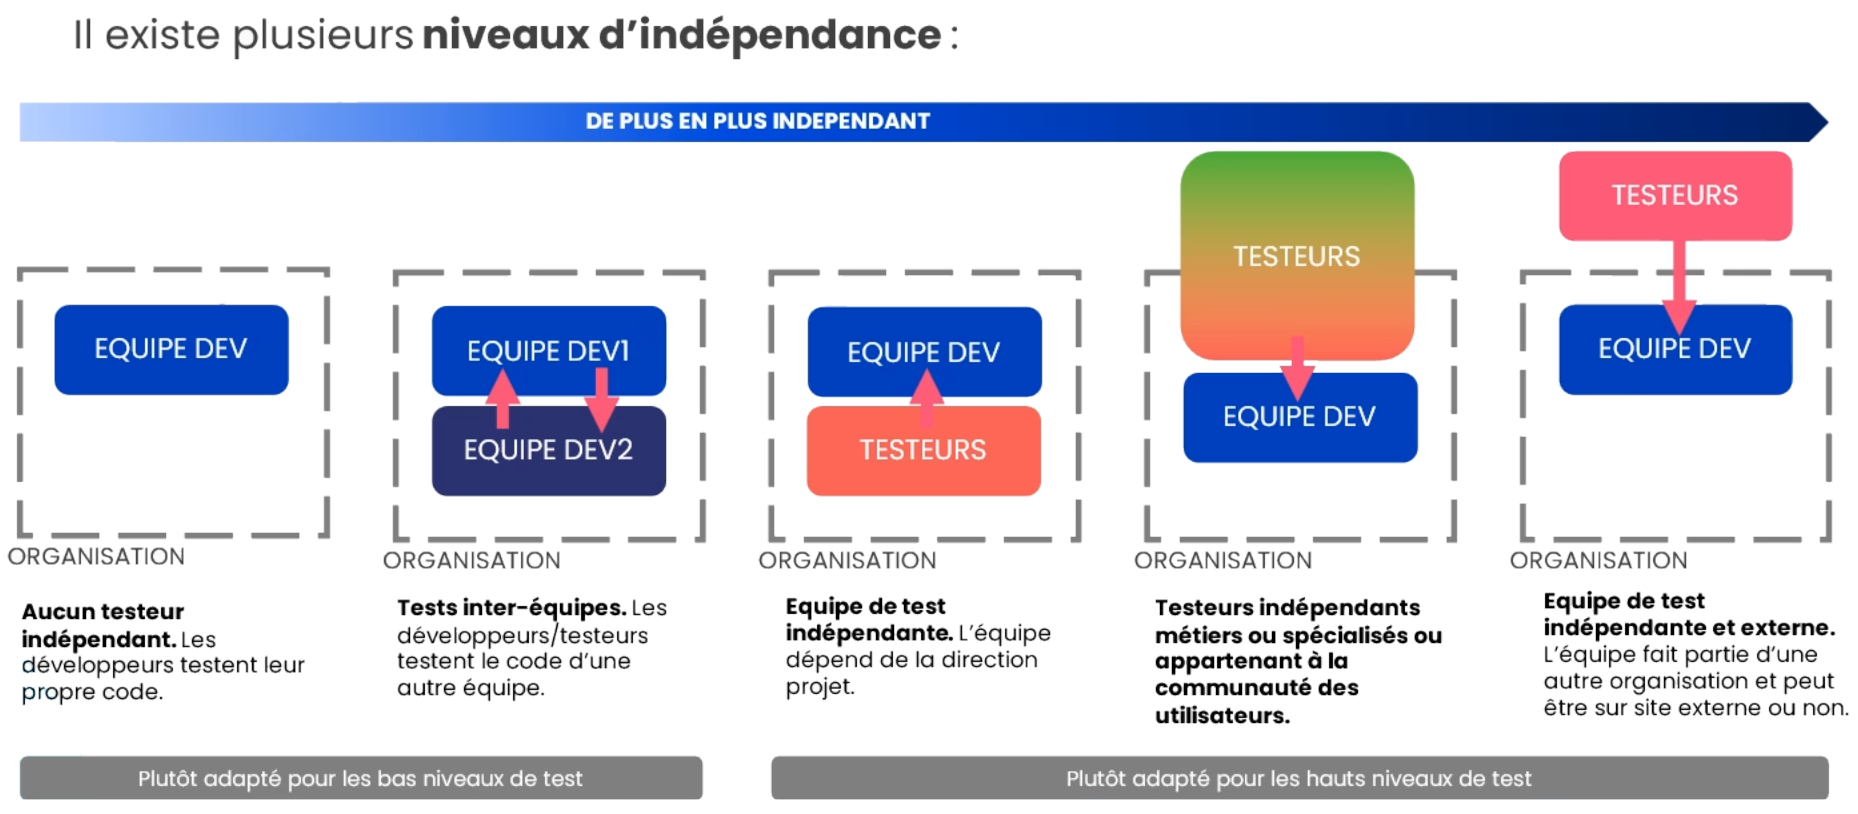
\includegraphics[width=0.9\textwidth]{images/Indépendance_01.png}
        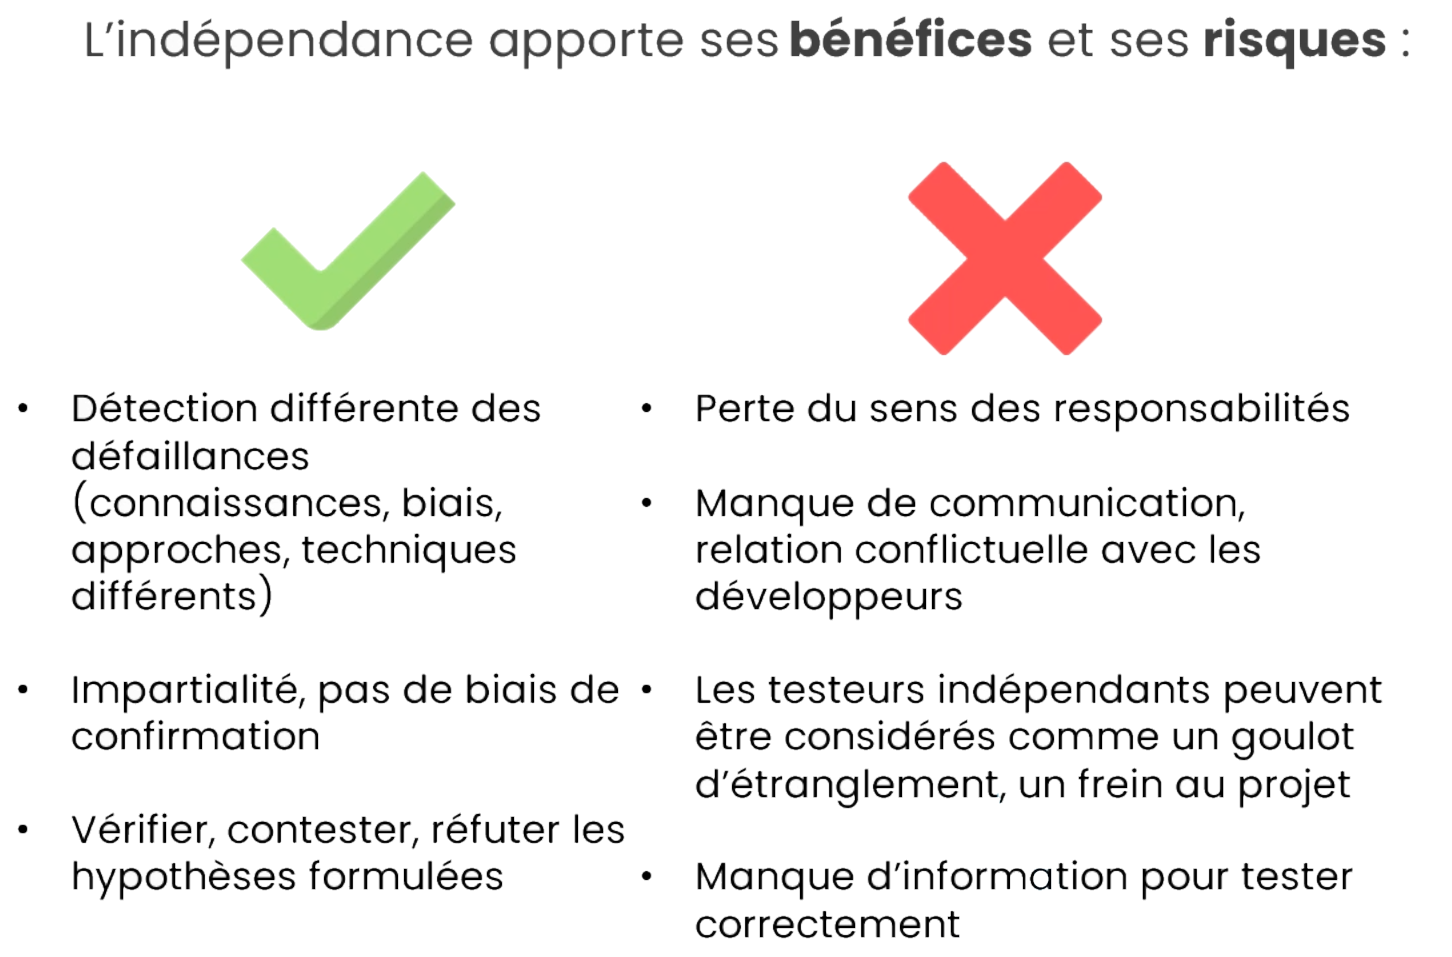
\includegraphics[width=0.9\textwidth]{images/Indépendance_02.png}
    \end{center}
    
	% \subsection{Démonstration}


\pagebreak
\section{TESTER PENDANT LE CYCLE DE DÉVELOPPEMENT LOGICIEL}

	\subsection{Les cycles de vie}

    \begin{center}
        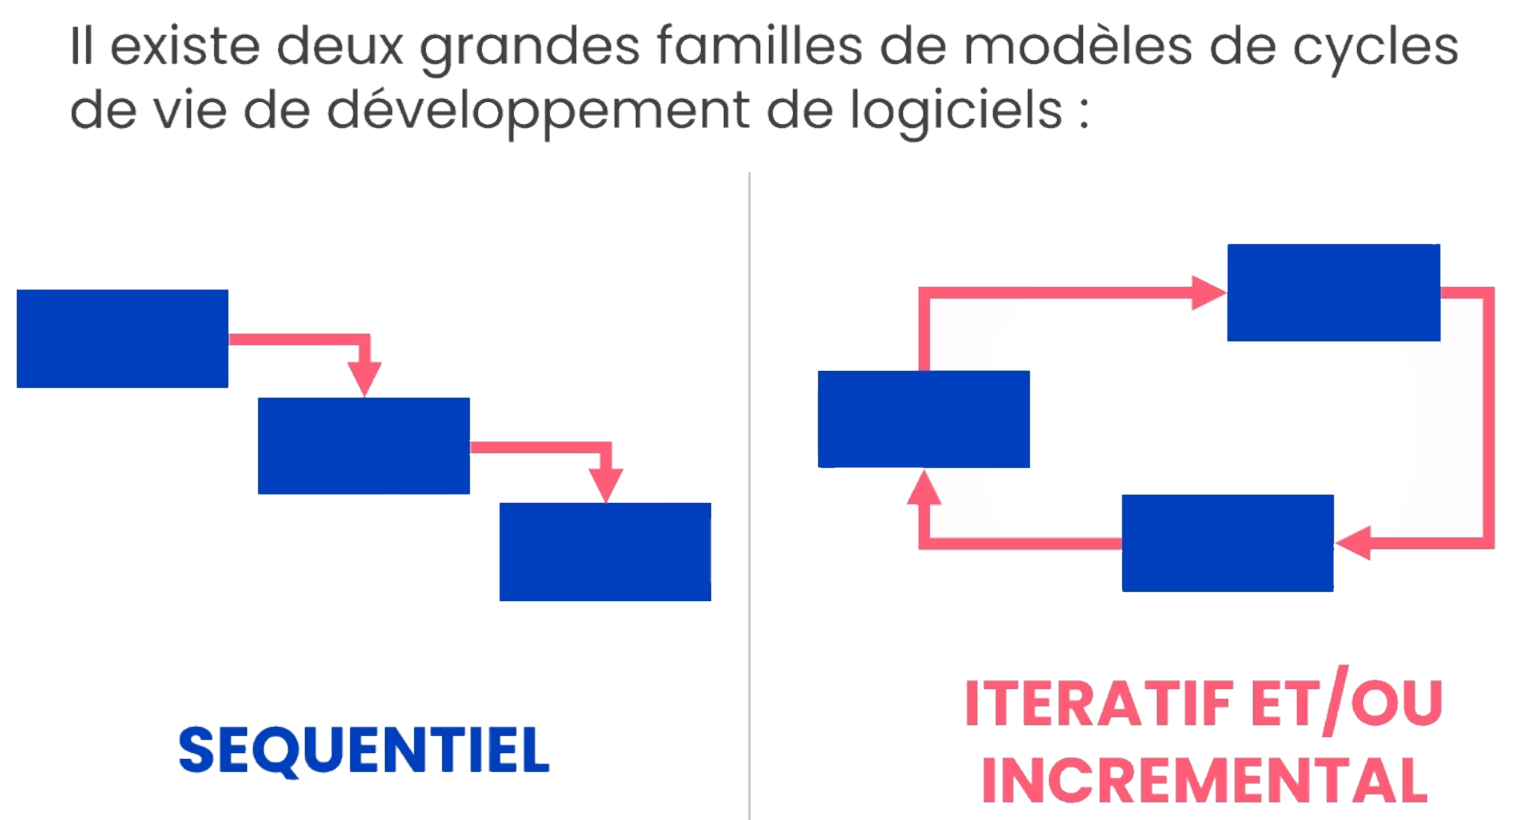
\includegraphics[width=0.9\textwidth]{images/Cycle_de_vie_01.png}
    \end{center}
        
        \subsubsection{Cycles de vie séquentiels}
        
    \begin{center}
        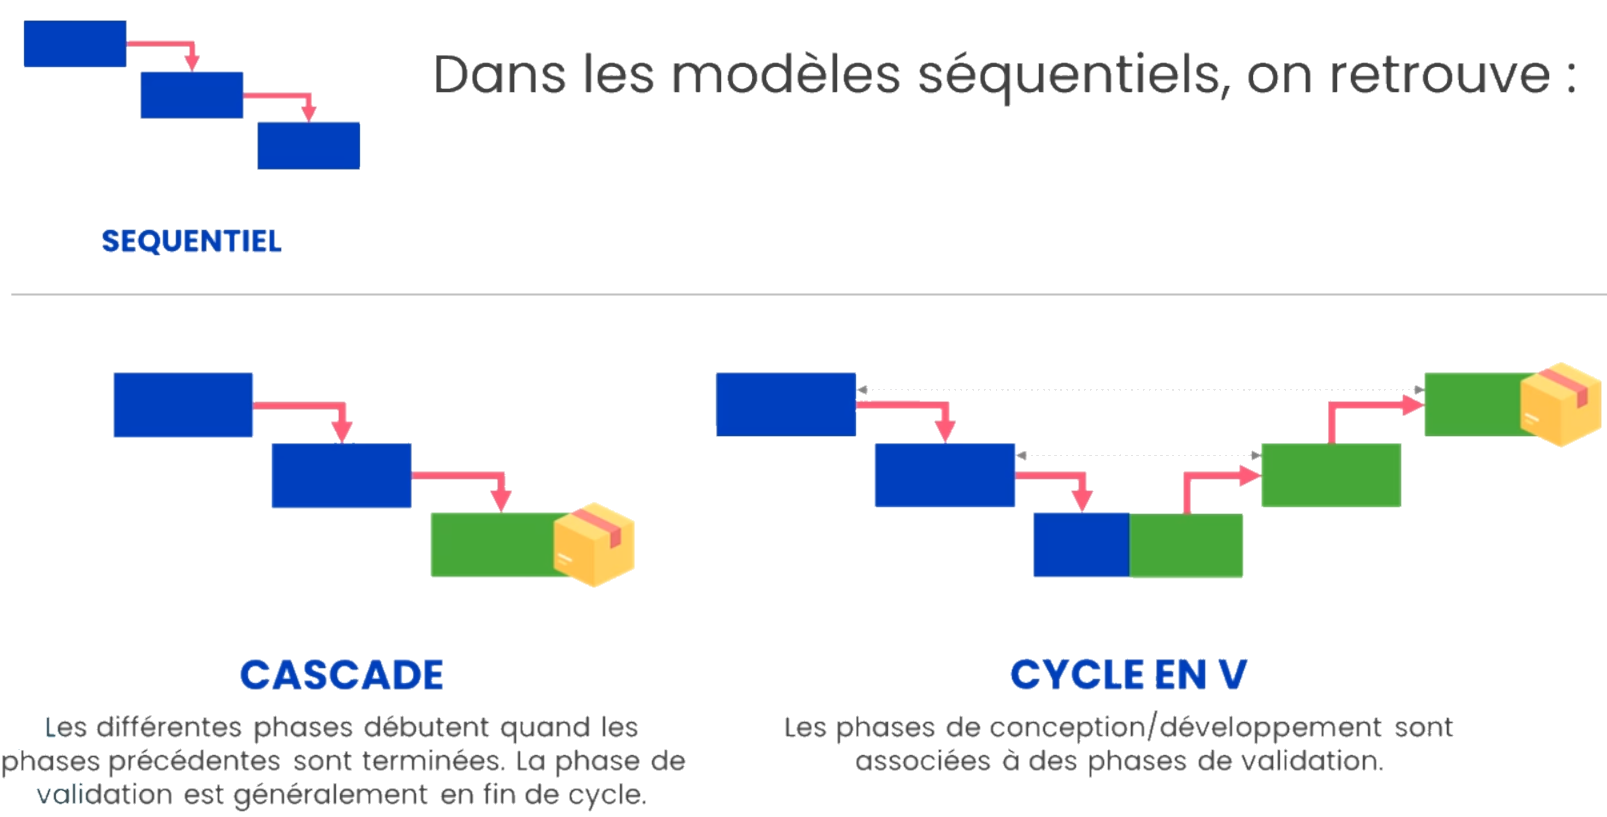
\includegraphics[width=0.9\textwidth]{images/Cycle_de_vie_02.png}
    \end{center}
    
    \subsubsection{Cycles de vie itératifs et/ou incrémentaux}
    
    \begin{center}
    	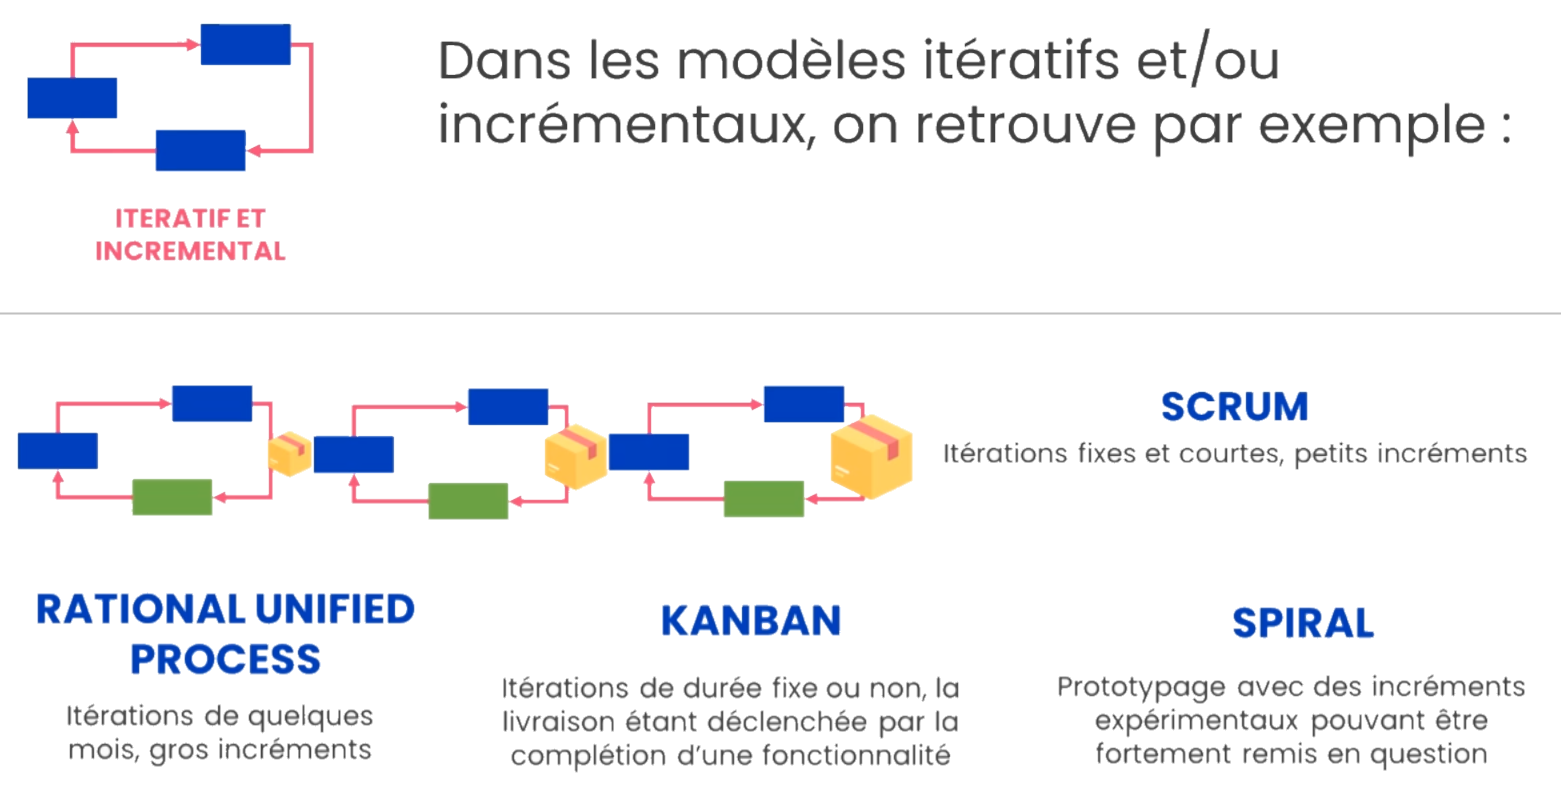
\includegraphics[width=0.9\textwidth]{images/Cycle_de_vie_03.png}
        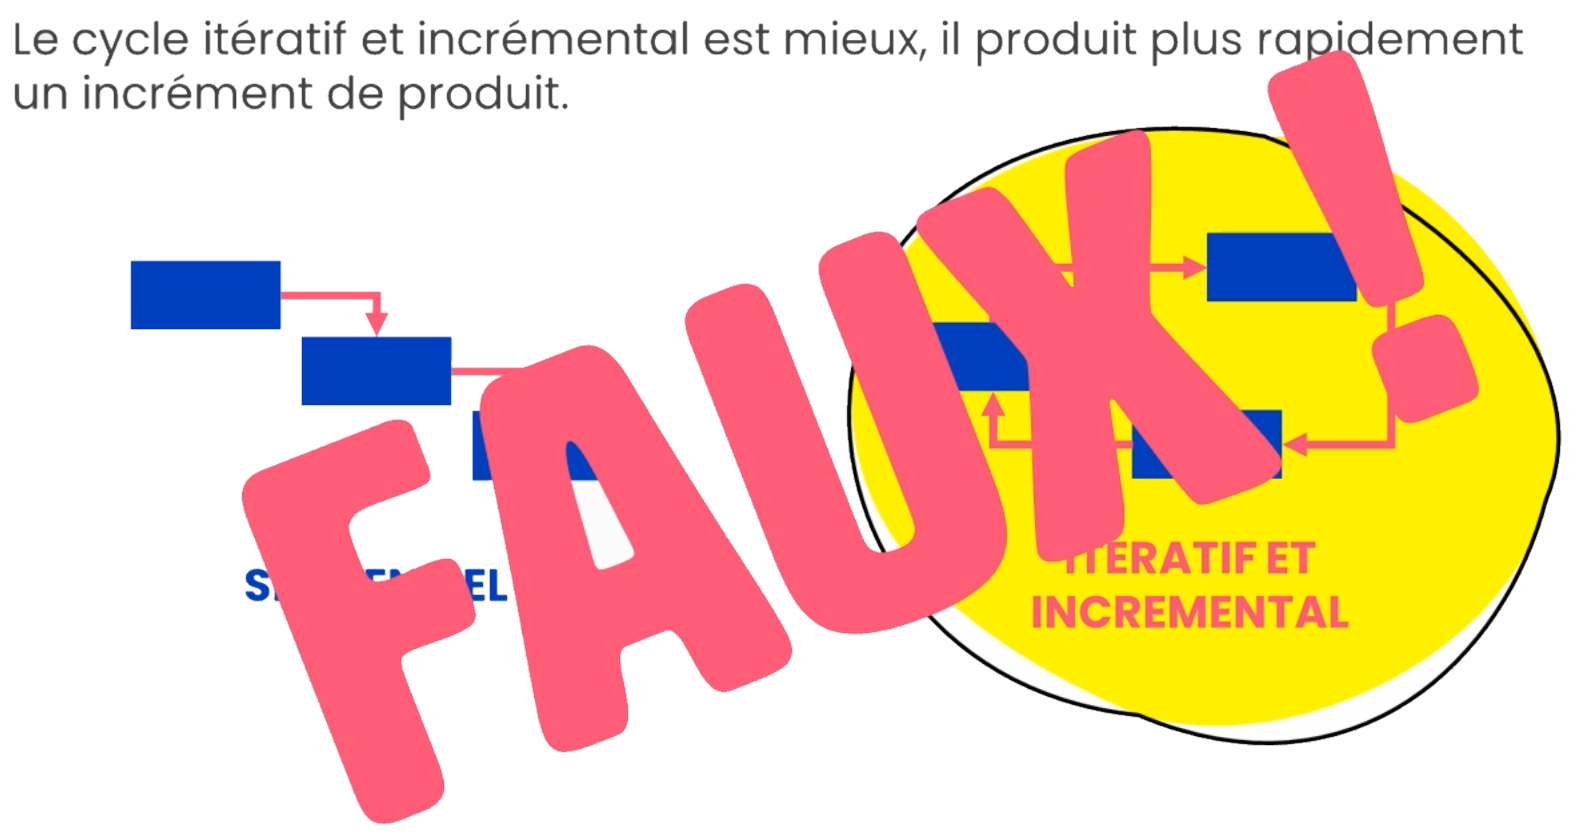
\includegraphics[width=0.9\textwidth]{images/Cycle_de_vie_04.png}
    \end{center}
    
    \subsubsection{Choix du cycles de vie}
    
    \begin{center}
        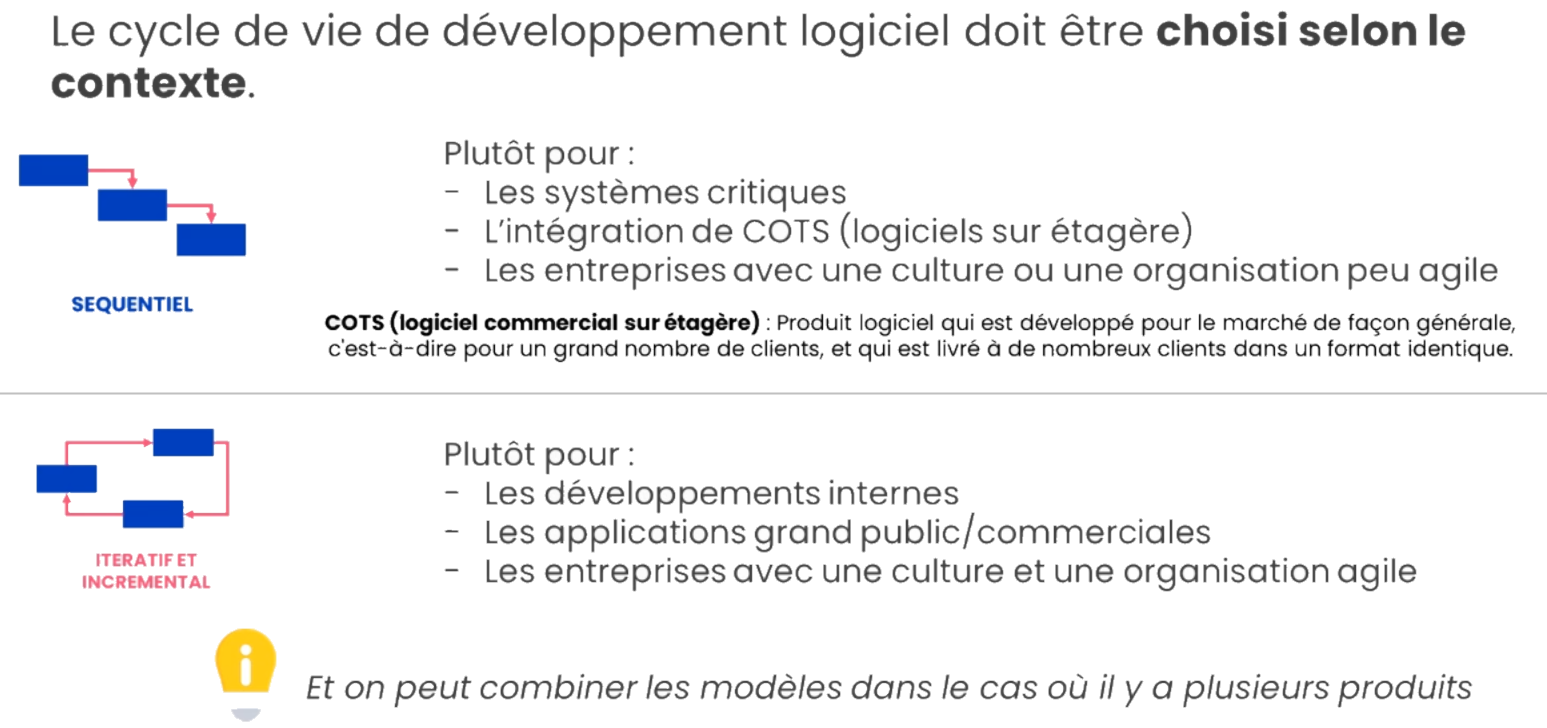
\includegraphics[width=0.9\textwidth]{images/Cycle_de_vie_05.png}
        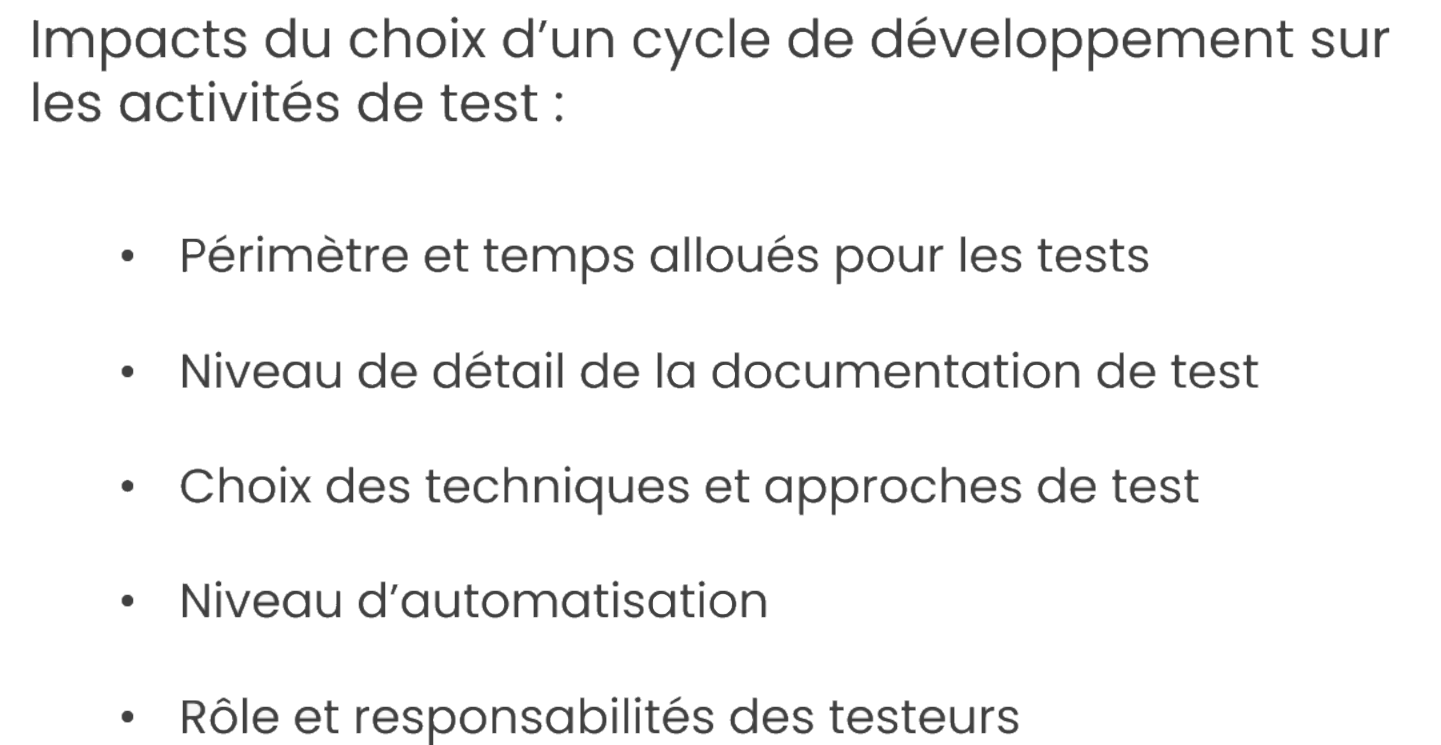
\includegraphics[width=0.9\textwidth]{images/Cycle_de_vie_06.png}
    \end{center}
    
	\subsection{Les bonnes pratiques}

    \begin{center}
        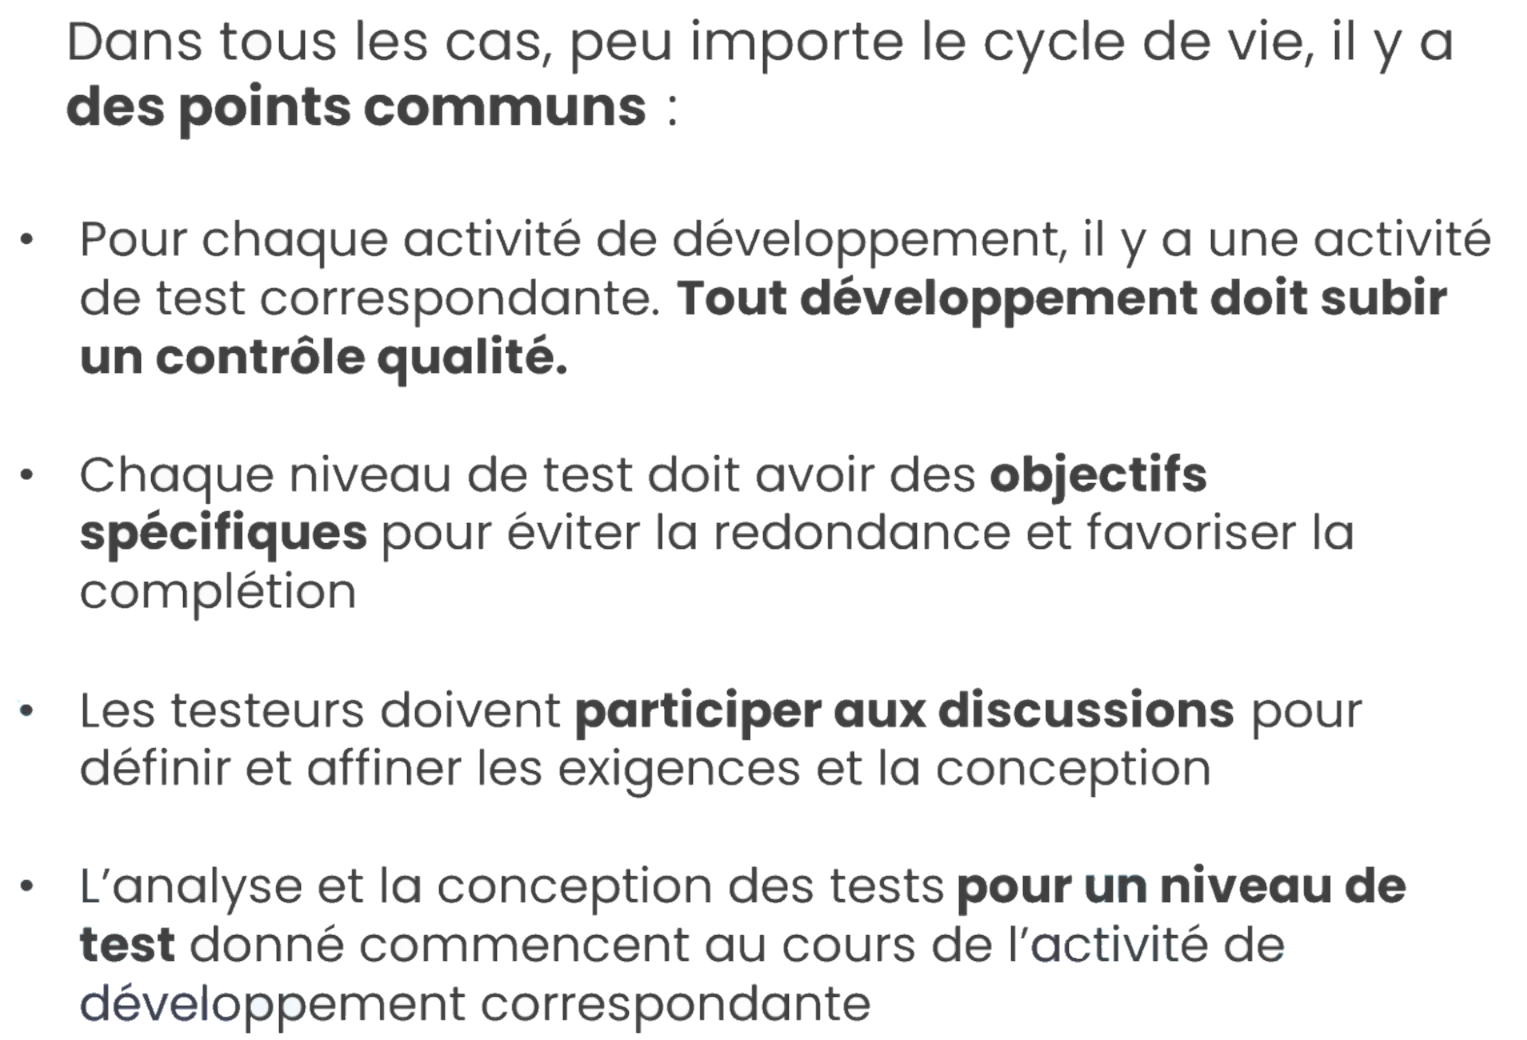
\includegraphics[width=0.9\textwidth]{images/Bonnes_pratiques.png}
    \end{center}

	\subsection{Le développement piloté par les tests}

    \begin{center}
        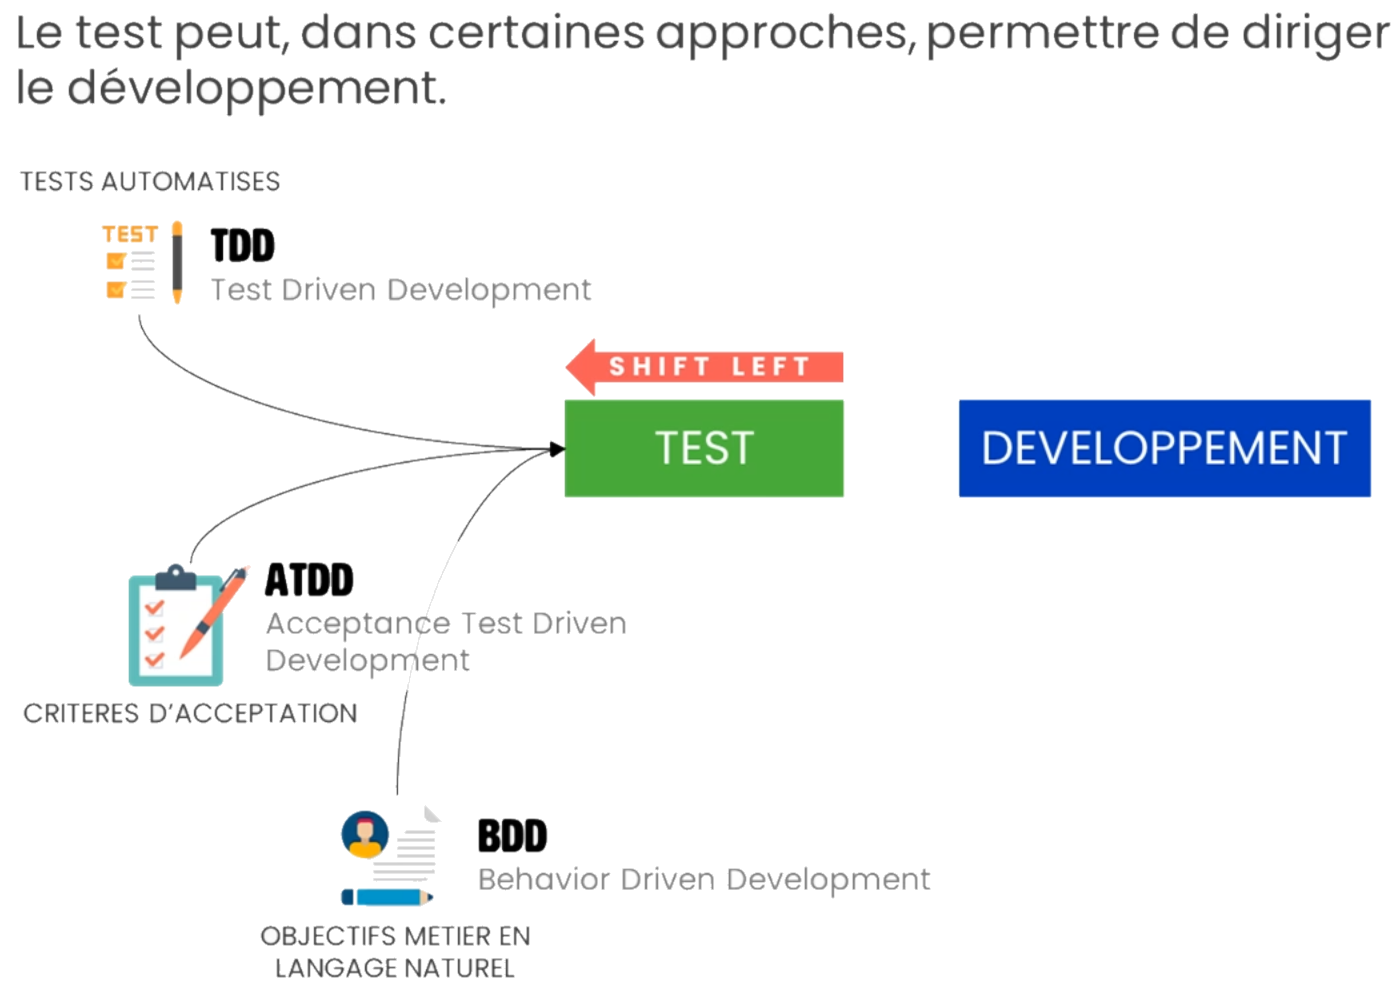
\includegraphics[width=0.9\textwidth]{images/tests_pilotés.png}
    \end{center}
    
    \alertinfo{\textbf{TDD}\newline Un Test Driven Development, ou développement piloté par les tests, est une méthodologie de développement logiciel dans laquelle les tests automatisés sont écrits avant le code fonctionnel nécessaire pour passer ces tests.}
    \alertinfo{\textbf{ATDD}\newline Acceptance Test Driven Development, est une méthodologie de développement logiciel qui implique une collaboration étroite entre les développeurs, les testeurs et les clients pour définir des tests d’acceptation avant de commencer le développement. L’ATDD permet de mieux cibler les fonctionnalités à développer et fournit une documentation claire du comportement du logiciel pour les développeurs et les testeurs.}
    \alertinfo{\textbf{BDD}\newline Le Behaviour Test Development permet d’écrire des tests qui décrivent le comportement attendu du système et que tout le monde peux comprendre.}
            
	\subsection{Le DevOps et les tests}

    \begin{center}
        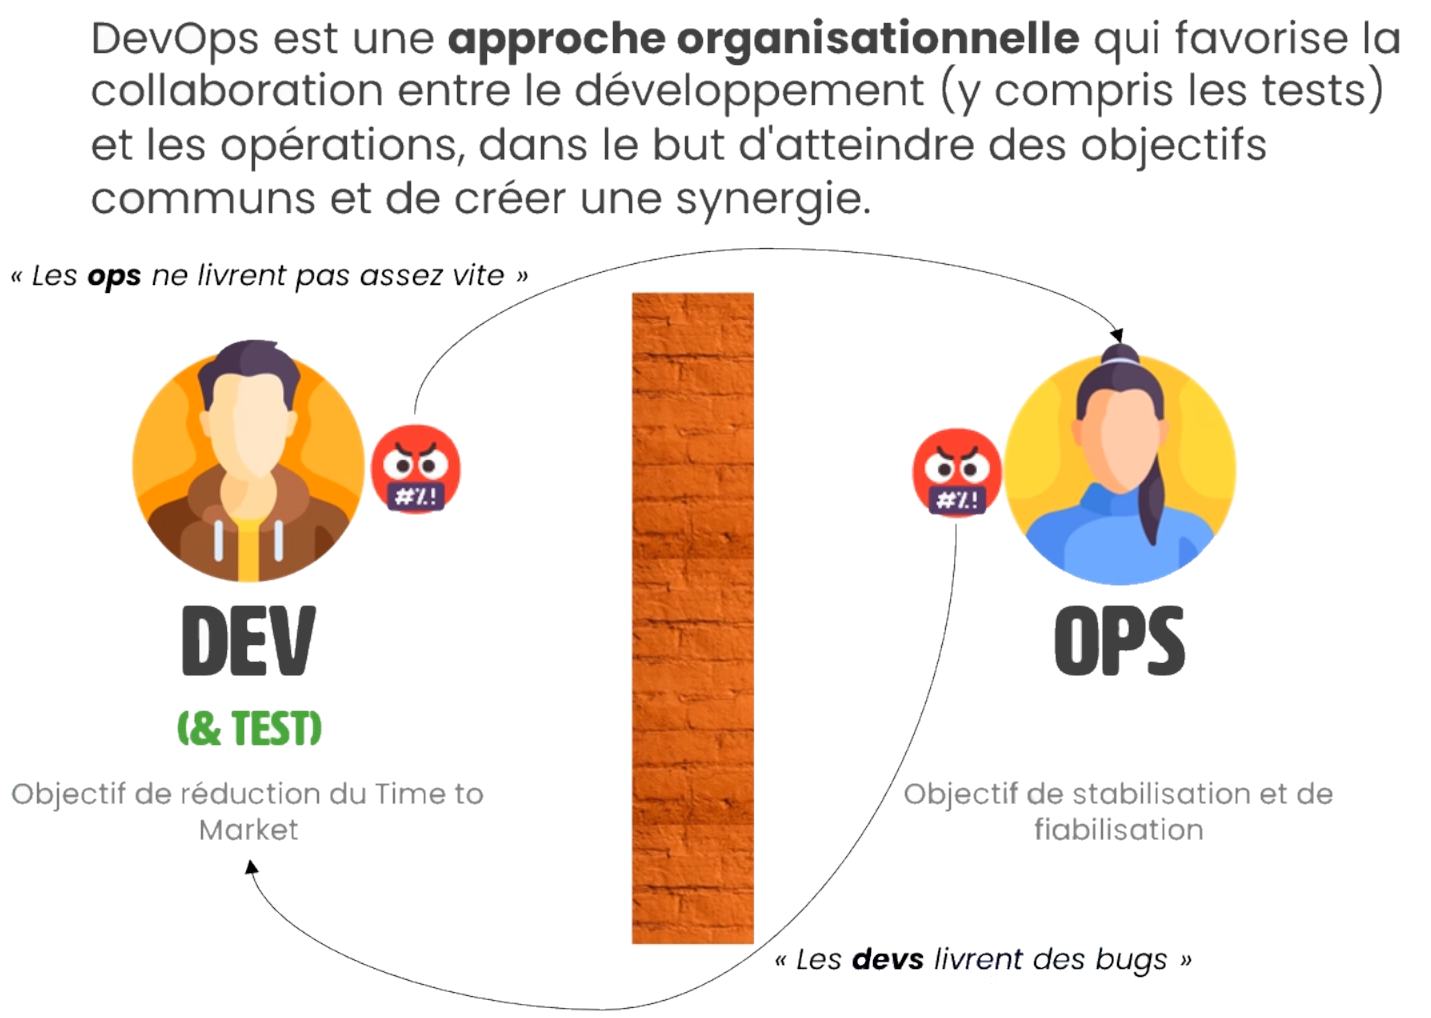
\includegraphics[width=0.9\textwidth]{images/devops_01.png}
        
\includegraphics[width=0.9\textwidth]{images/devops_02.png}
        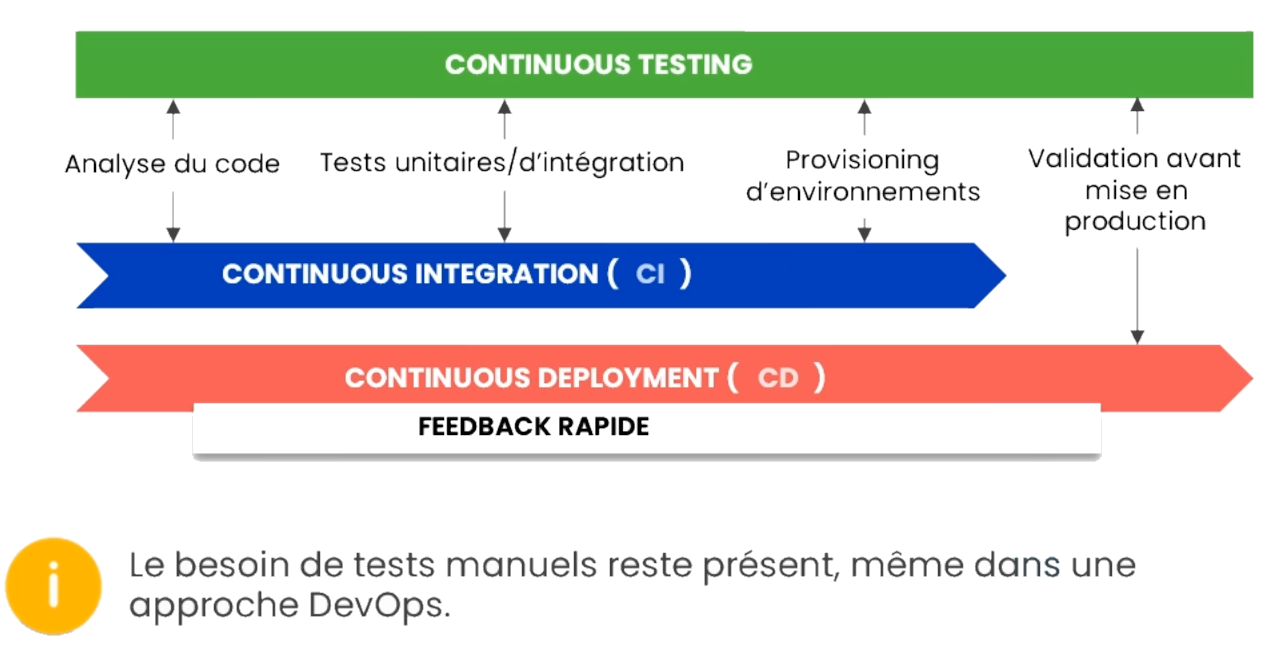
\includegraphics[width=0.9\textwidth]{images/devops_03.png}
    \end{center}
    
        \alertinfo{\textbf{CI/CD}\newline La pratique de l'intégration continue (CI) consiste à intégrer automatiquement et régulièrement les modifications de code dans un référentiel de code source partagé. La distribution et/ou le déploiement continus (CD) désignent quant à eux un processus en deux volets qui englobe l'intégration, les tests et la distribution des modifications apportées au code. La distribution continue se limite au déploiement automatique dans les environnements de production, alors que le déploiement continu publie automatiquement les mises à jour dans ces environnements.}
        
    \begin{center}
        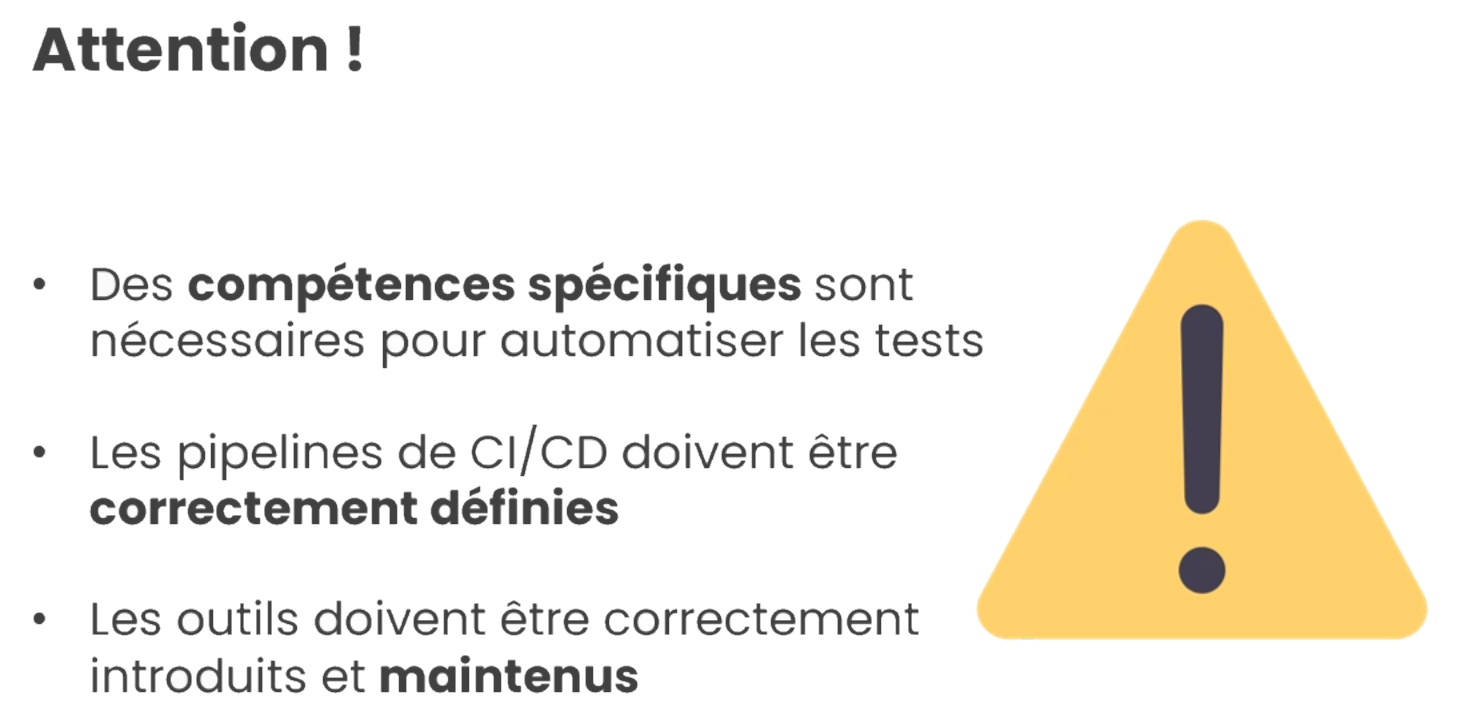
\includegraphics[width=0.9\textwidth]{images/devops_04.png}
    \end{center}

	\subsection{Le shift-left}

    \begin{center}
        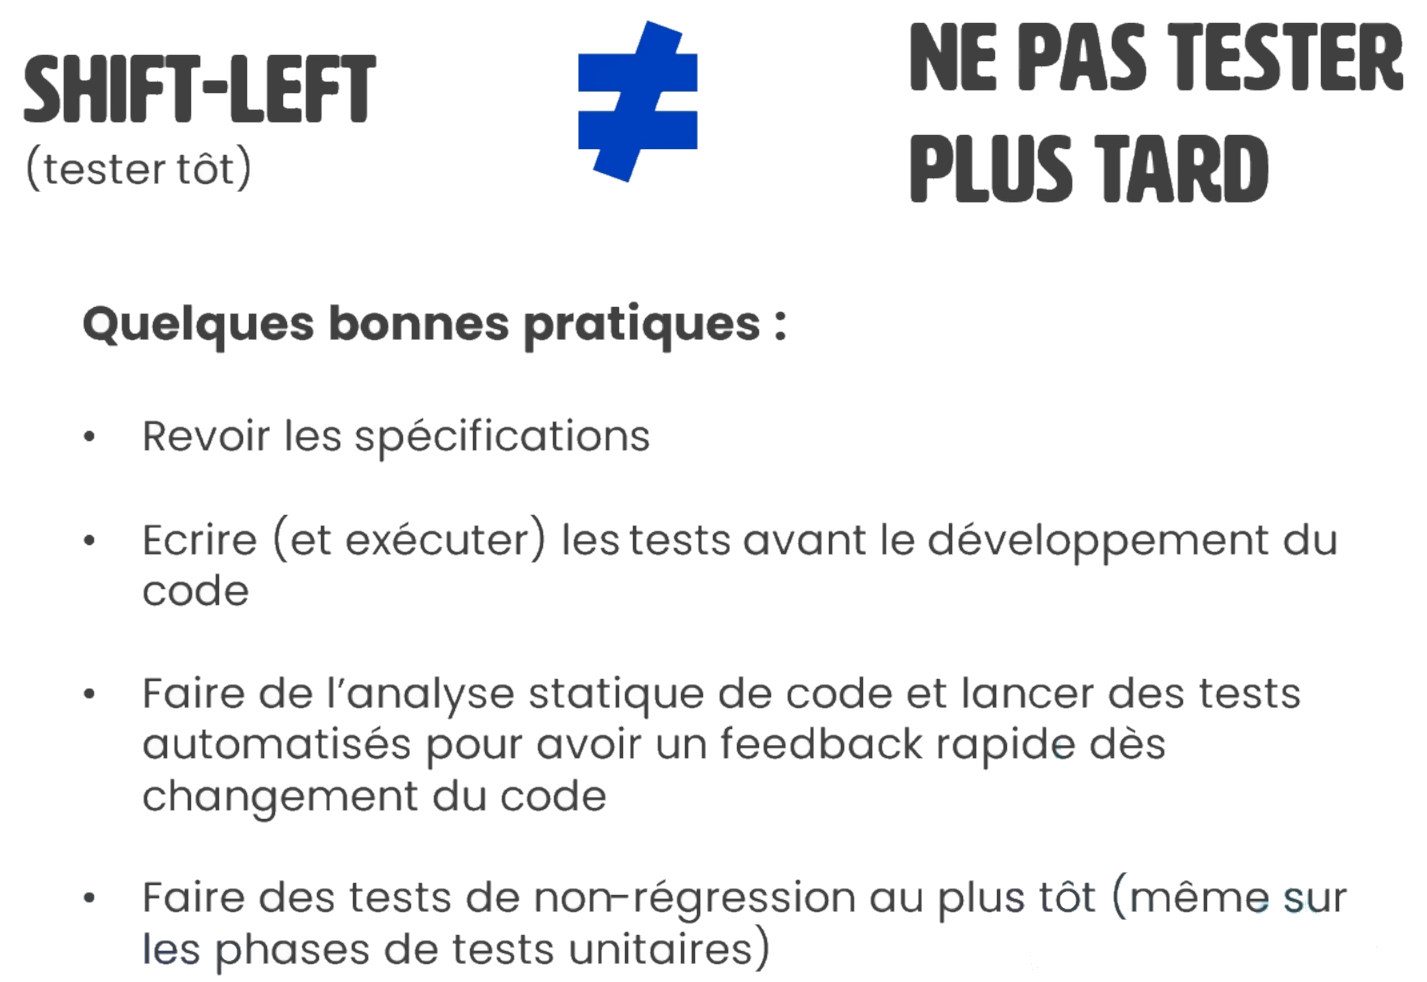
\includegraphics[width=0.9\textwidth]{images/shift_left.png}
    \end{center}
    
	\subsection{La rétrospective}

    \begin{center}
        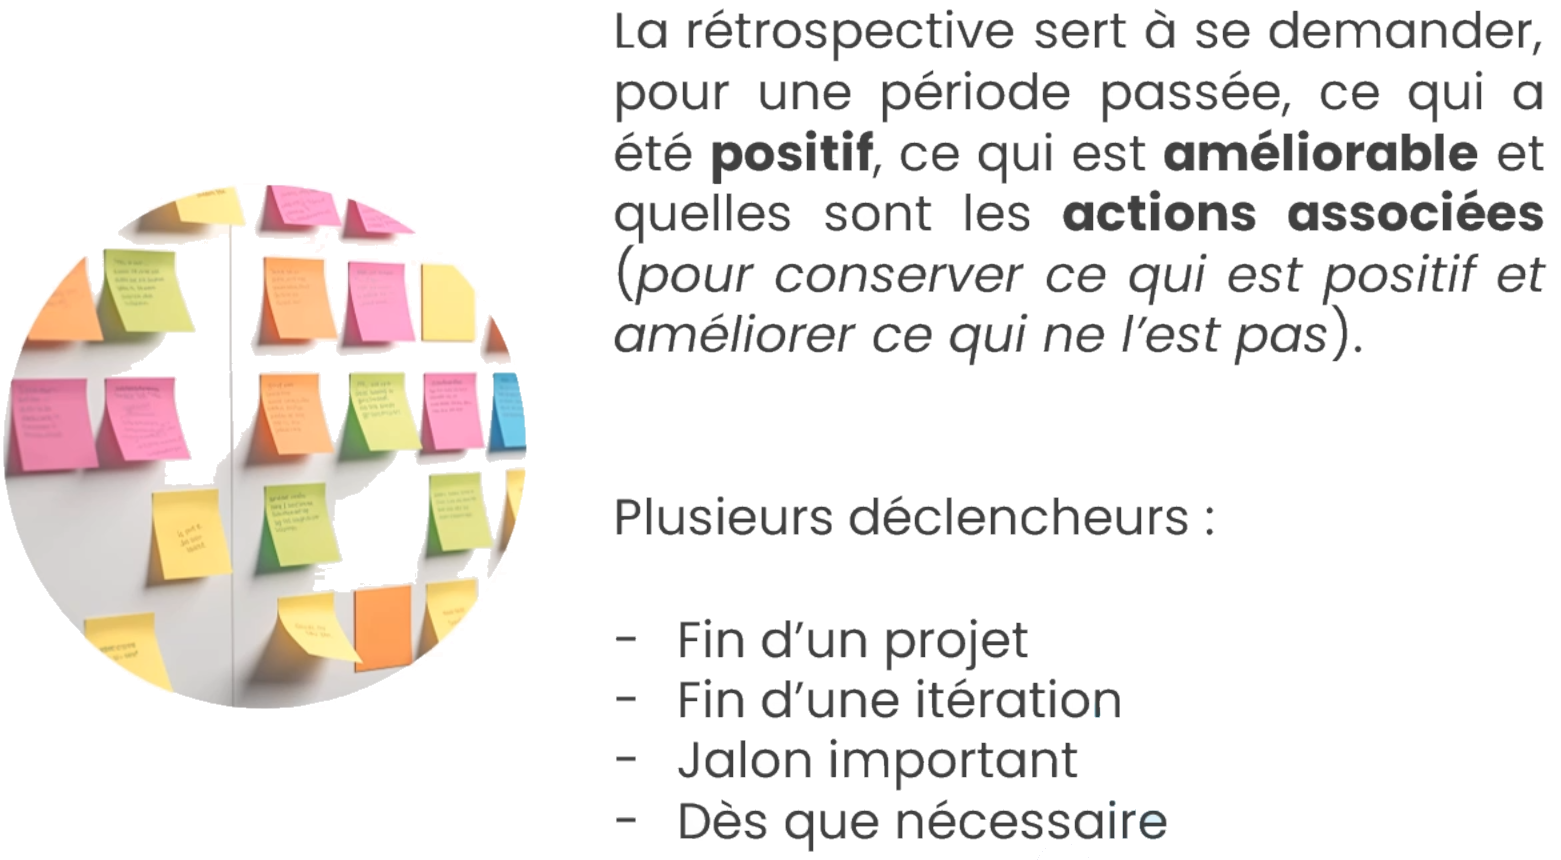
\includegraphics[width=0.9\textwidth]{images/retrospective_01.png}
        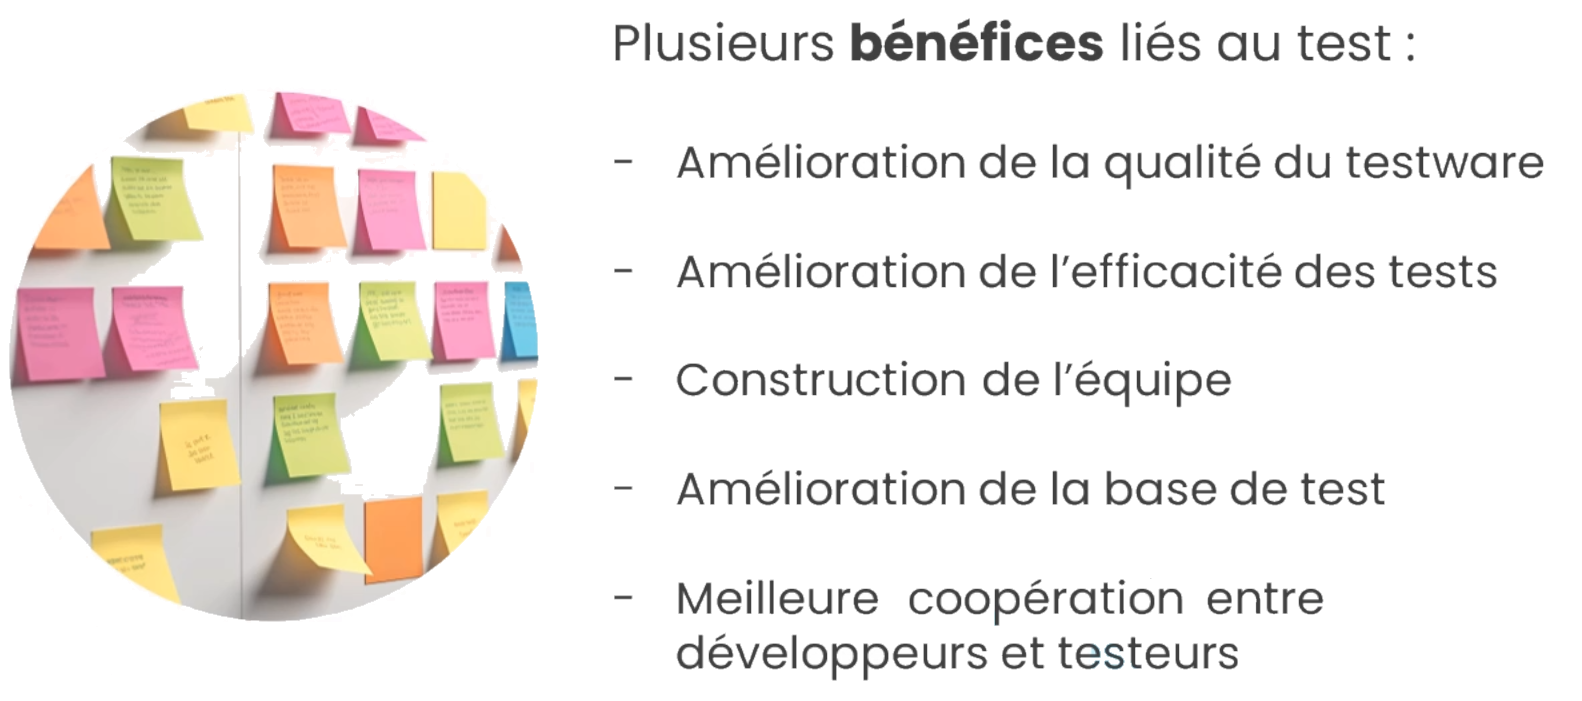
\includegraphics[width=0.9\textwidth]{images/retrospective_02.png}
    \end{center}
    
	\subsection{Les niveaux de test}

    \begin{center}
        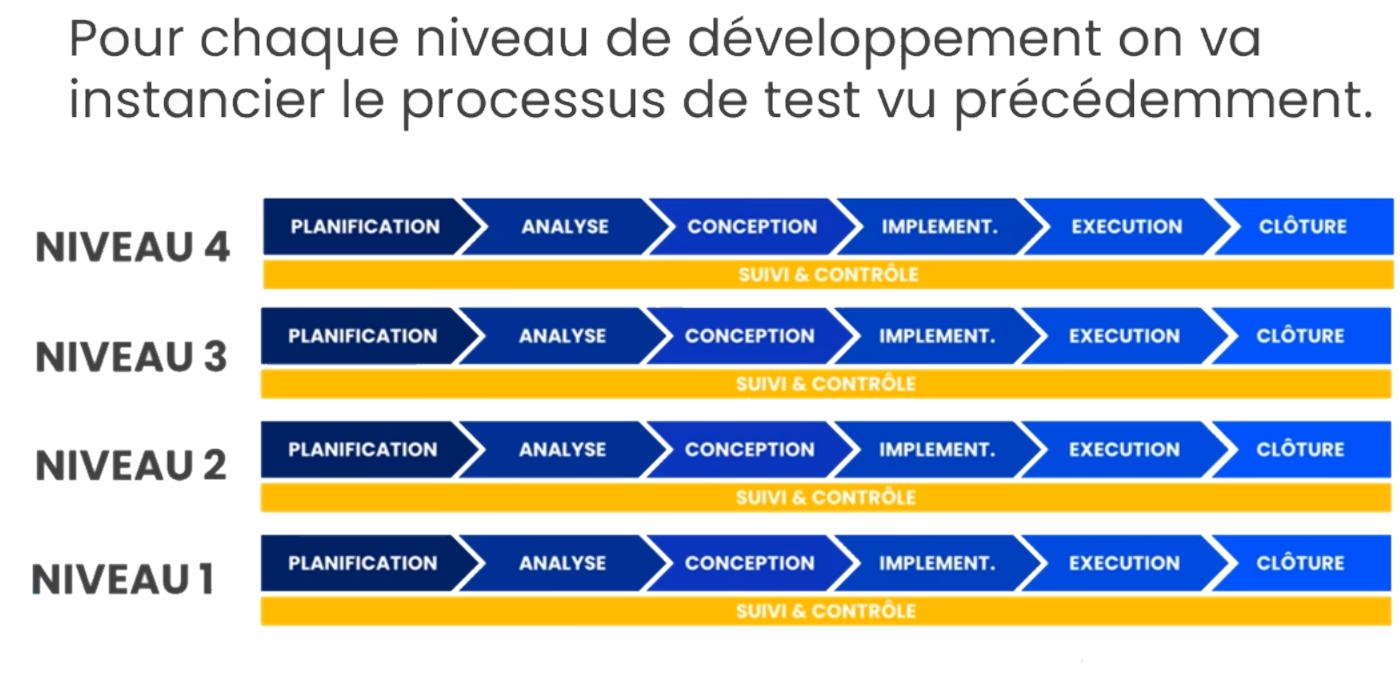
\includegraphics[width=0.9\textwidth]{images/niveaux_01.png}
        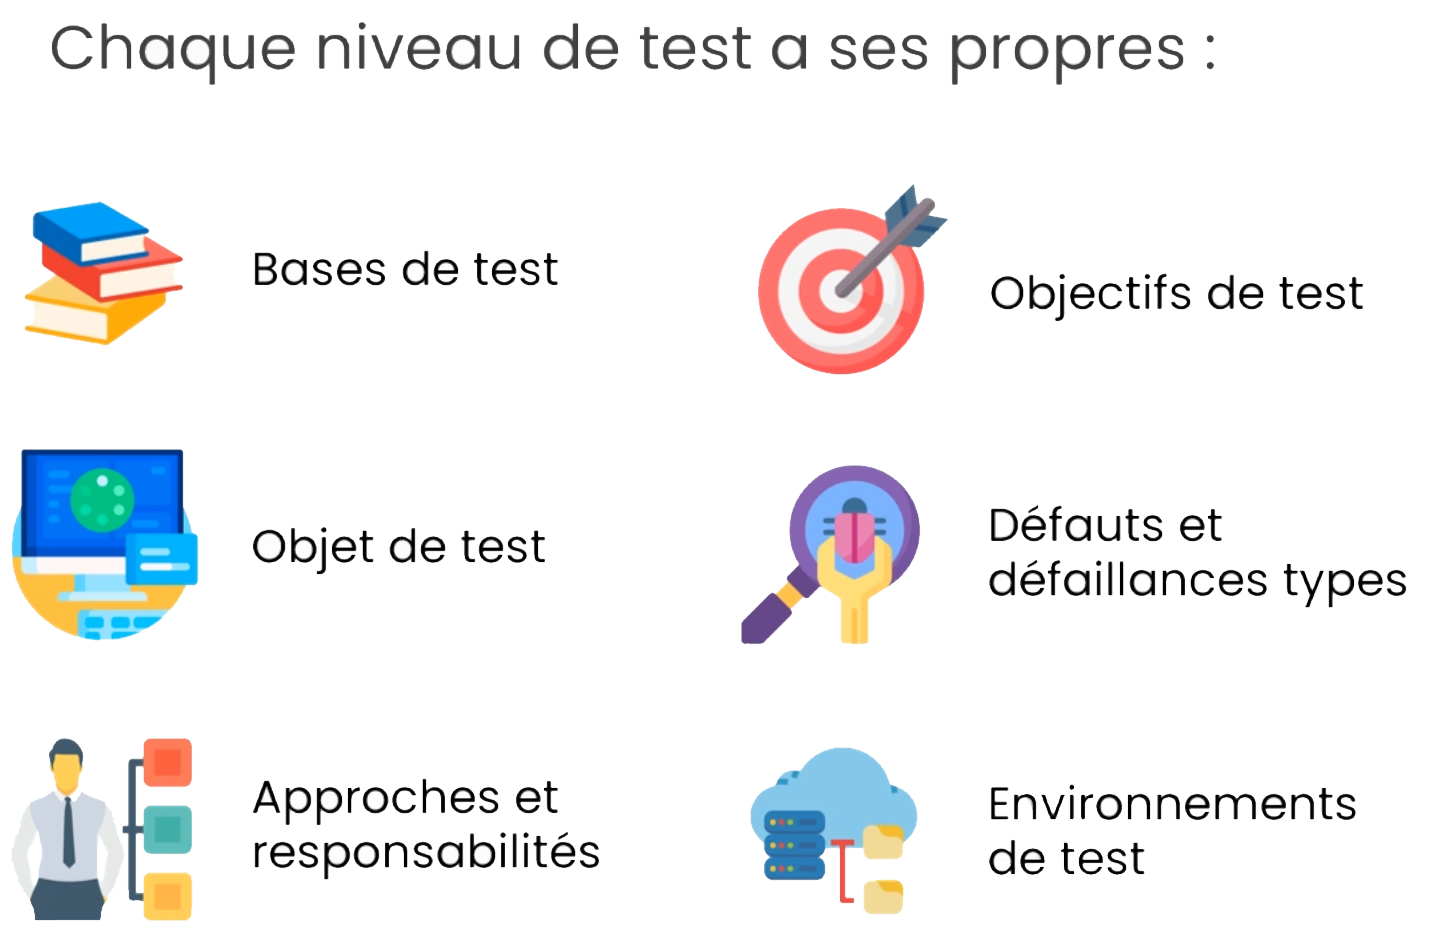
\includegraphics[width=0.9\textwidth]{images/niveaux_02.png}
        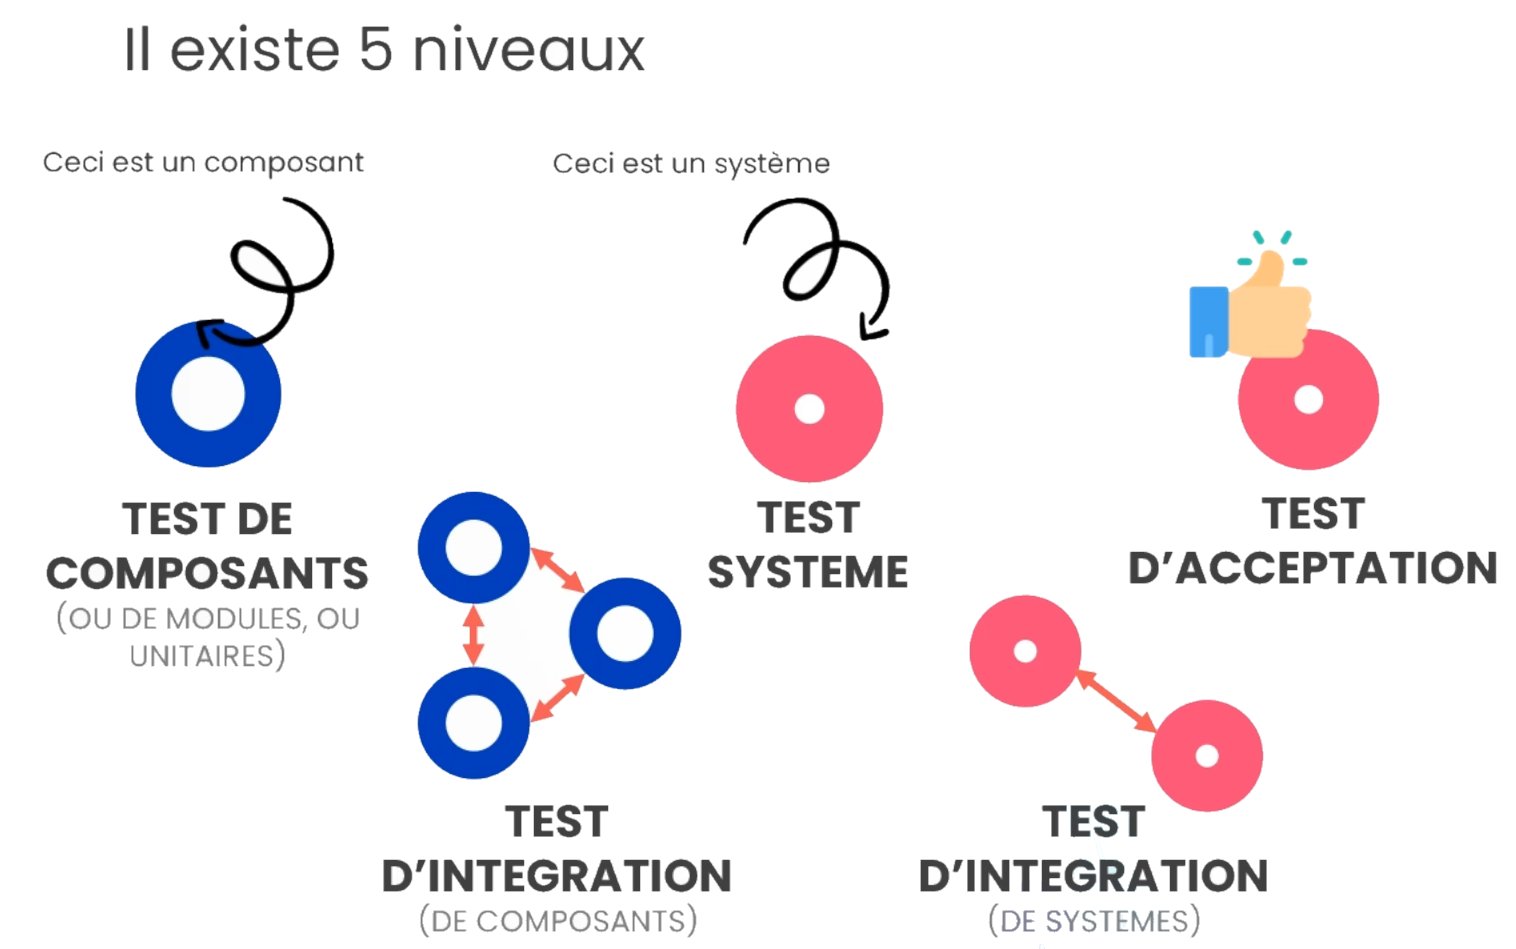
\includegraphics[width=0.9\textwidth]{images/niveaux_03.png}
        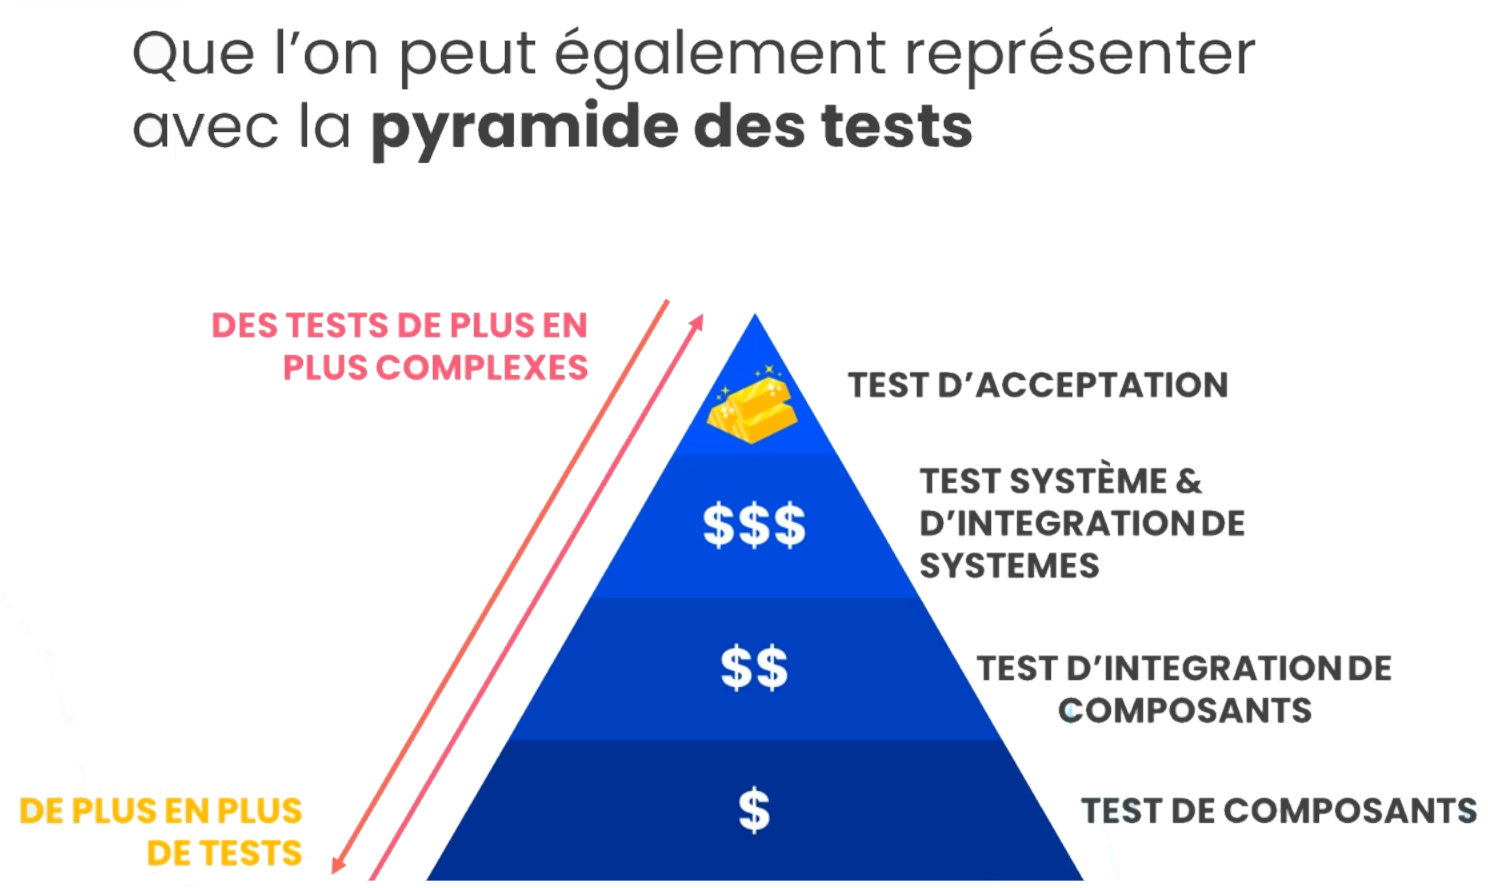
\includegraphics[width=0.9\textwidth]{images/niveaux_04.png}
    \end{center}
    
	\subsection{Les tests composant}

    \begin{center}
        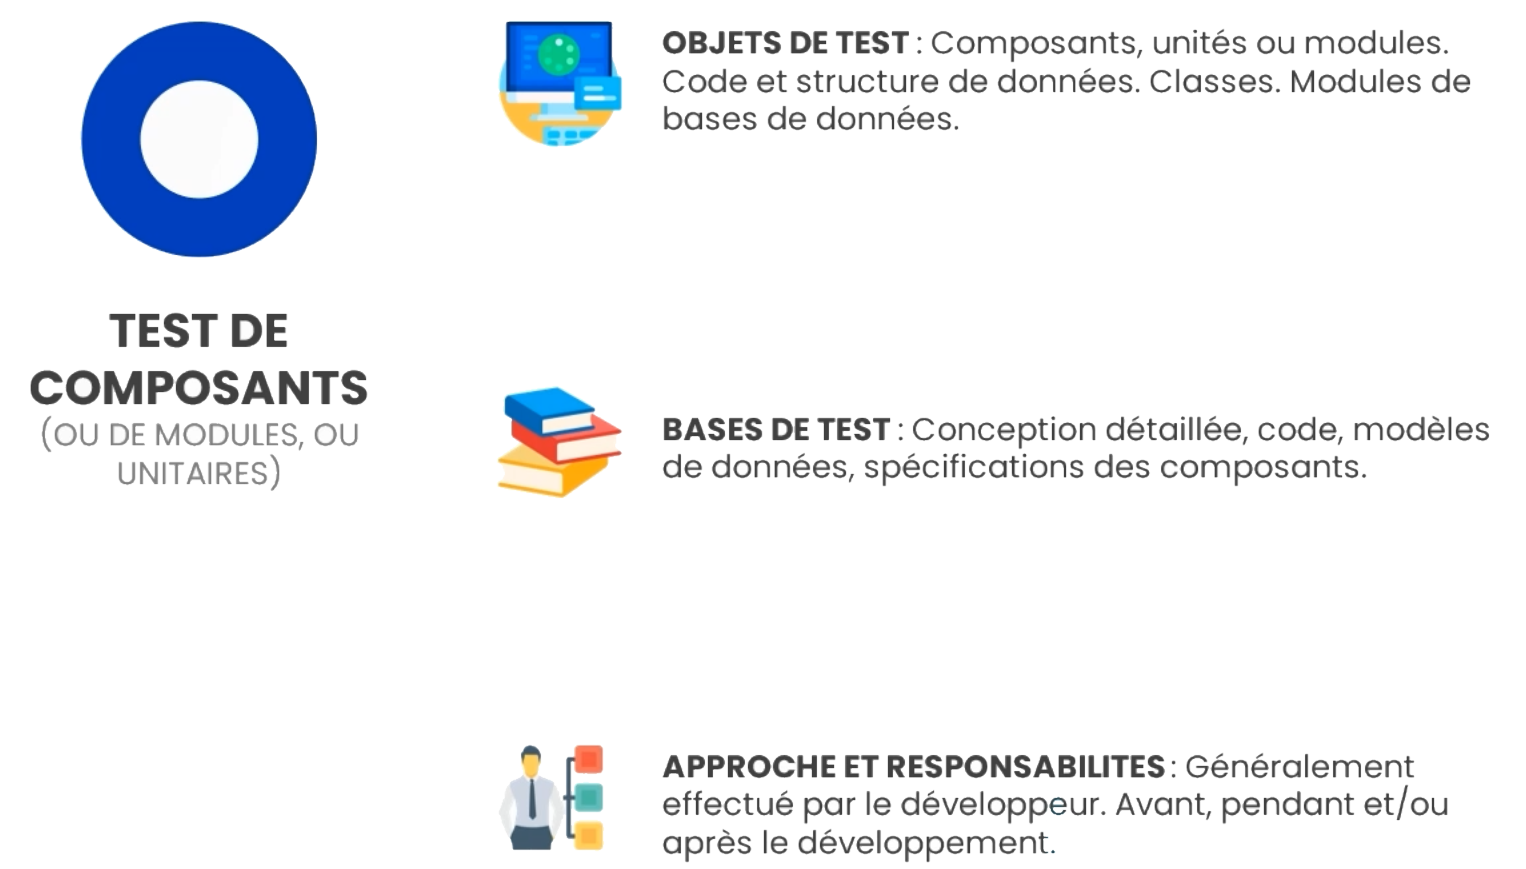
\includegraphics[width=0.9\textwidth]{images/composants_01.png}
        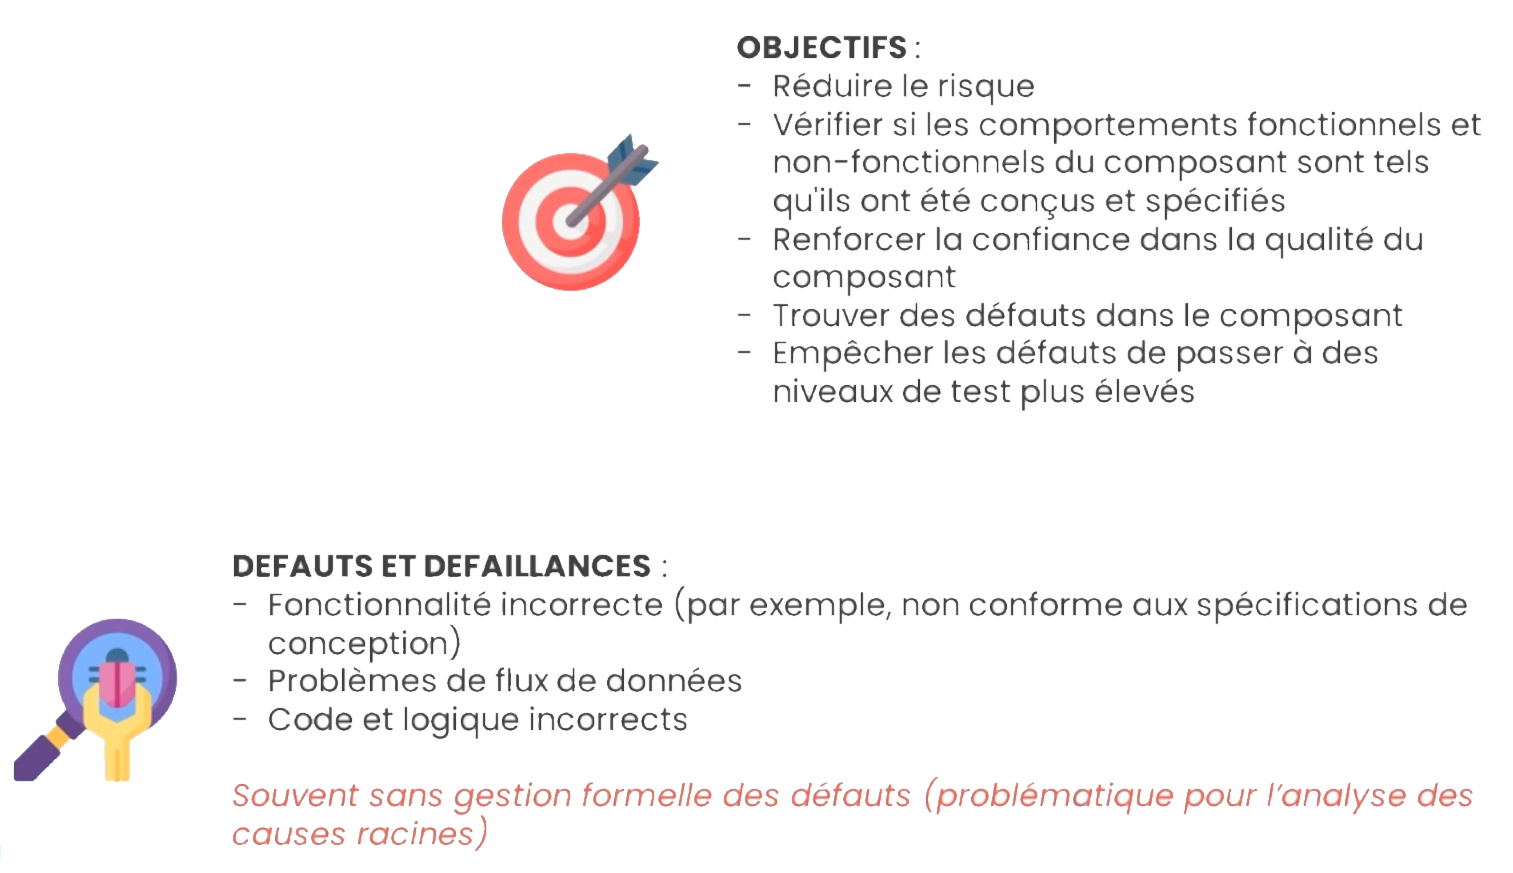
\includegraphics[width=0.9\textwidth]{images/composants_02.png}
        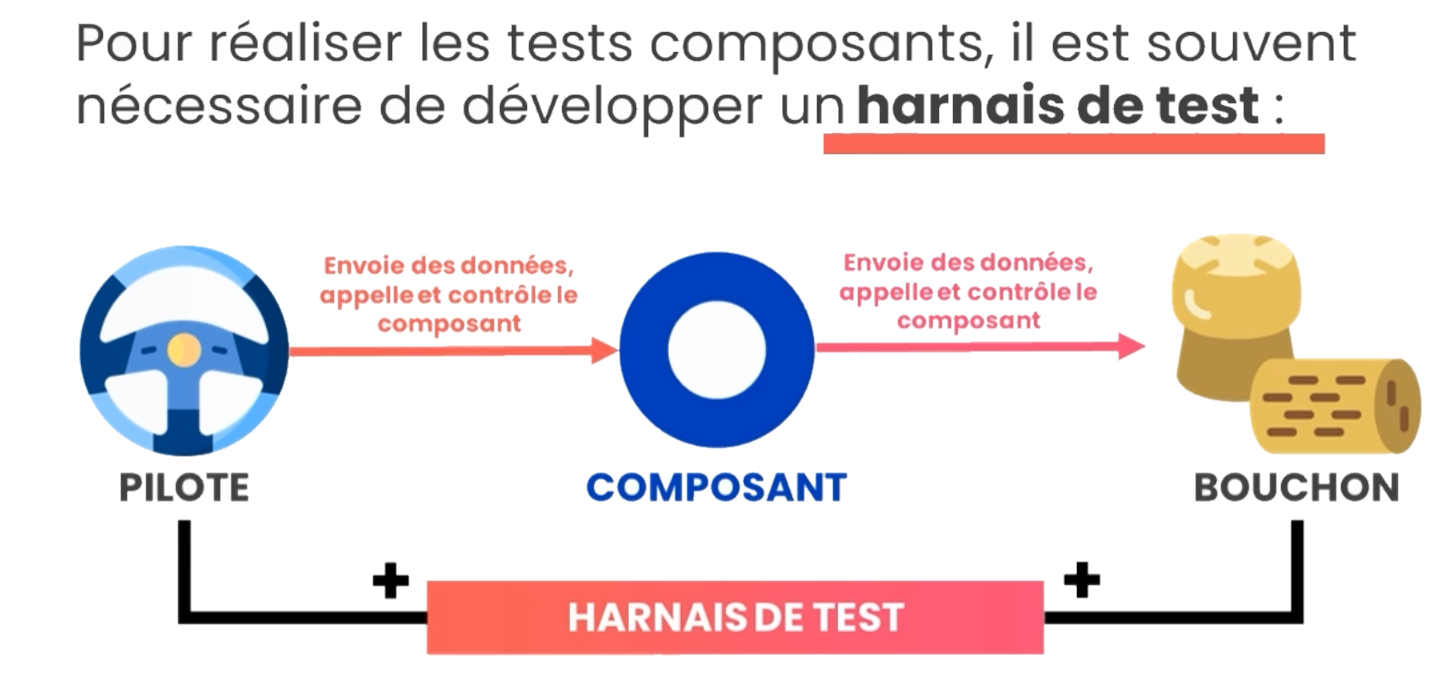
\includegraphics[width=0.9\textwidth]{images/composants_03.png}
    \end{center}
    
	\subsection{Les tests d'intégration}

    \begin{center}
        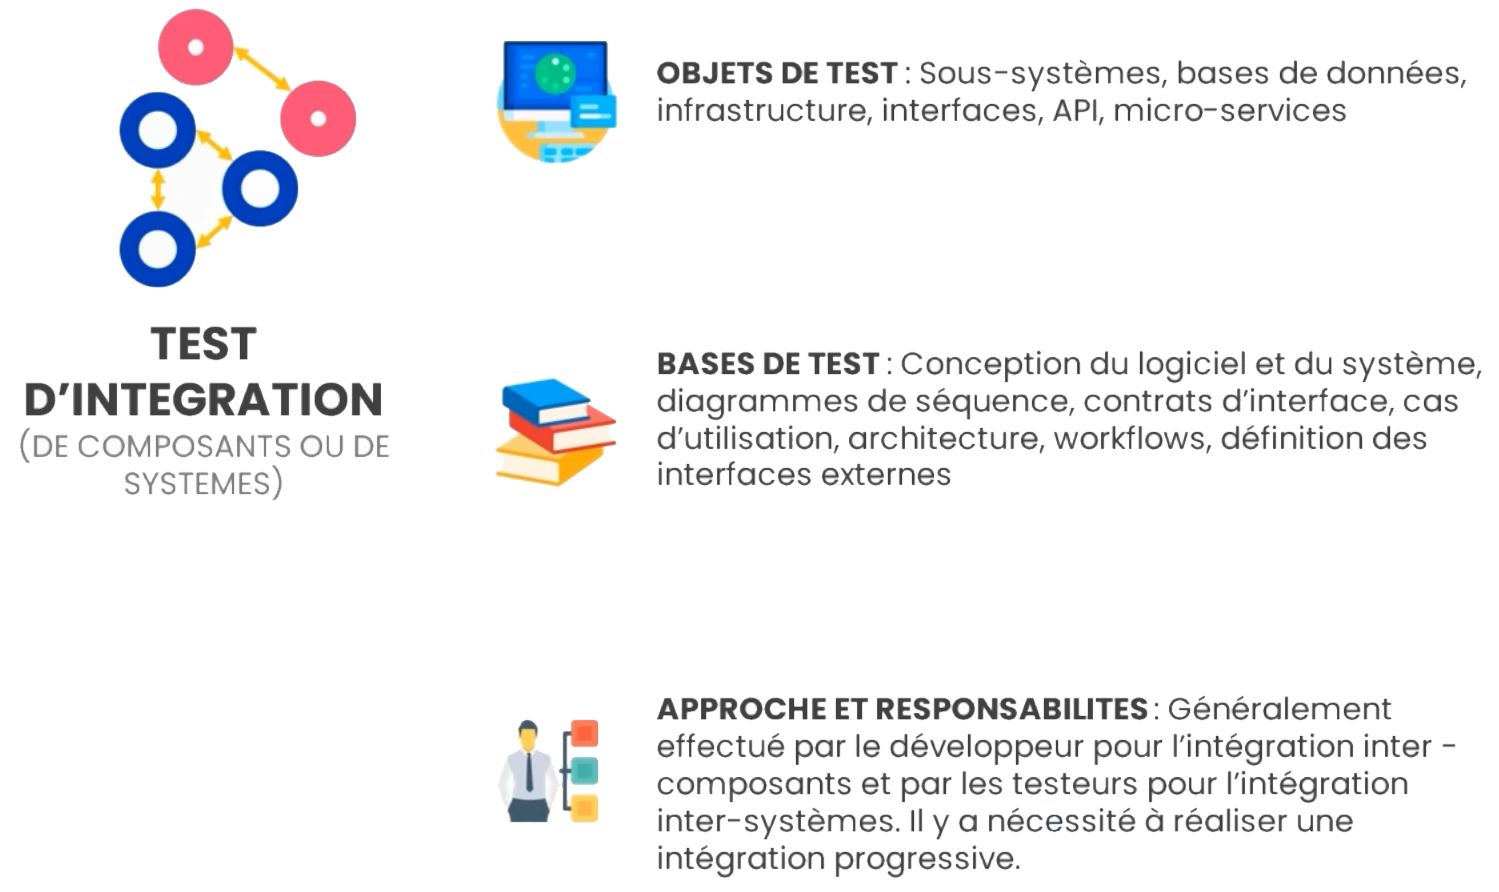
\includegraphics[width=0.9\textwidth]{images/intégration_01.png}
        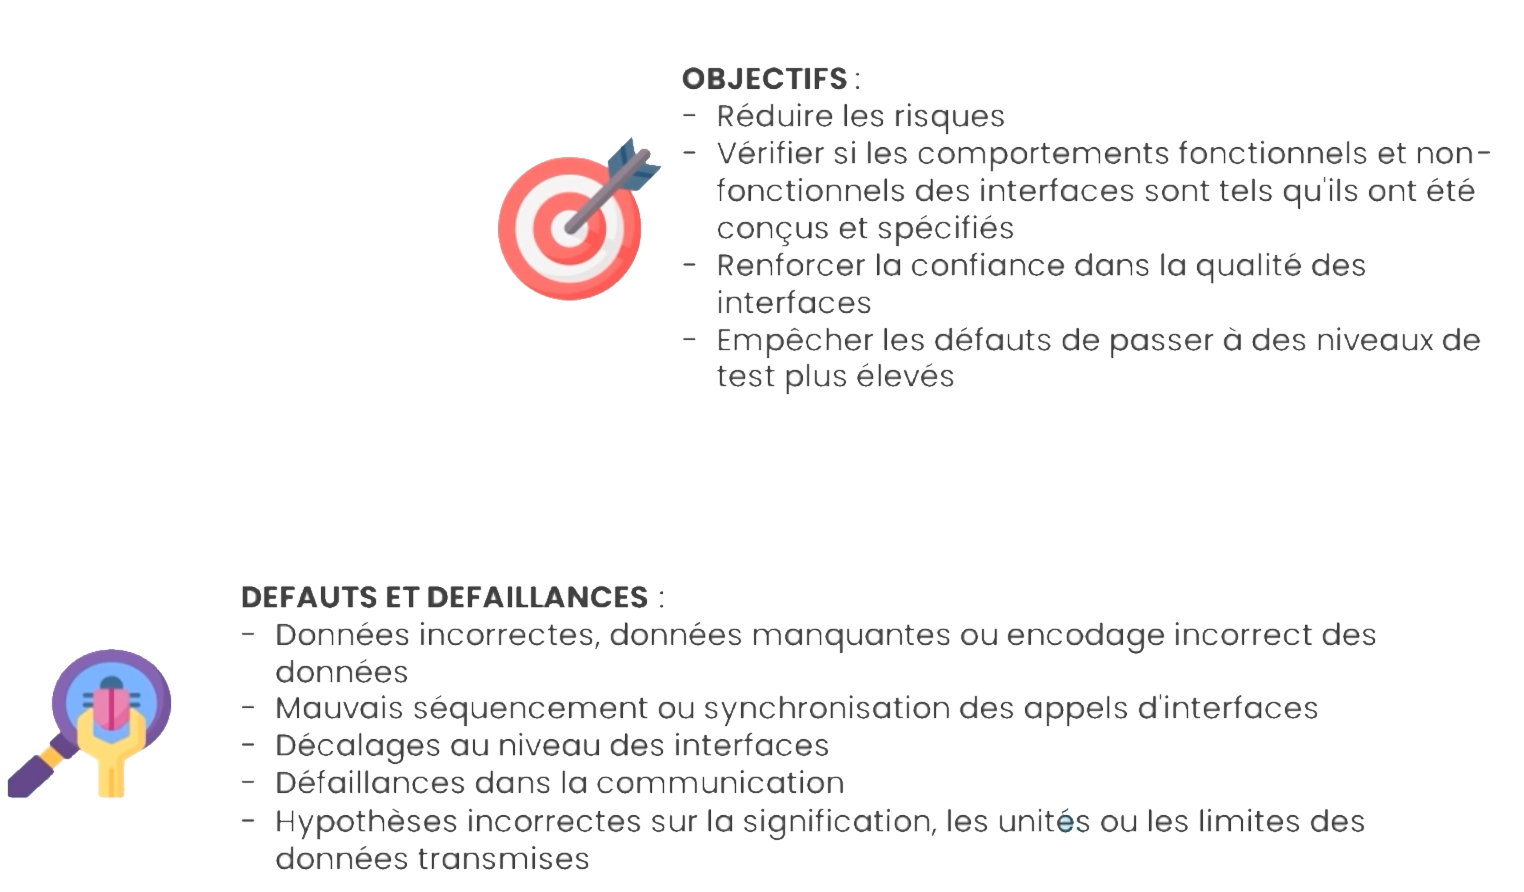
\includegraphics[width=0.9\textwidth]{images/intégration_02.png}
    \end{center}
    
	\subsection{Les tests système}

    \begin{center}
        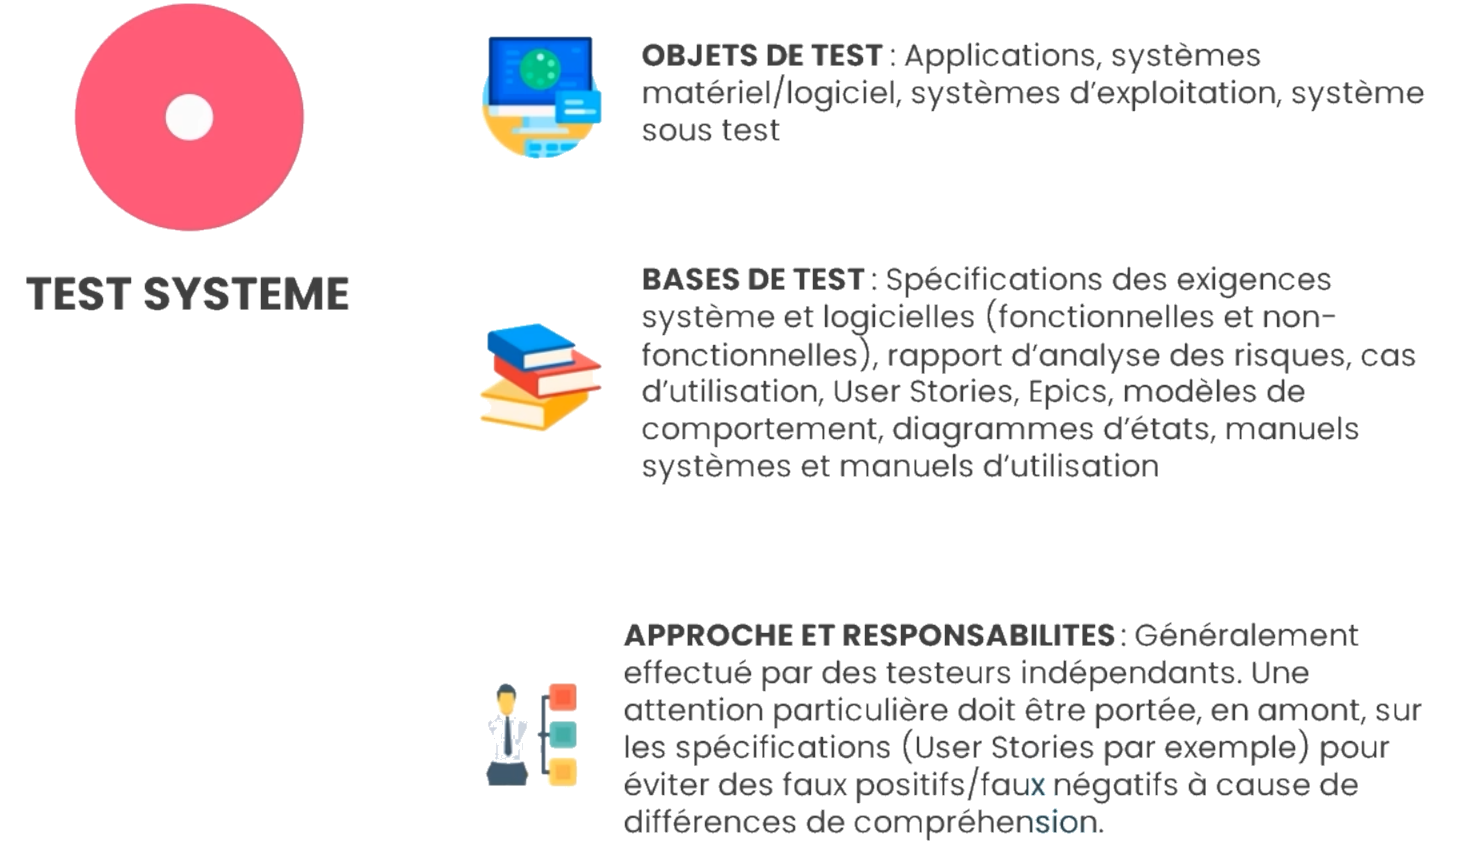
\includegraphics[width=0.9\textwidth]{images/systeme_01.png}
        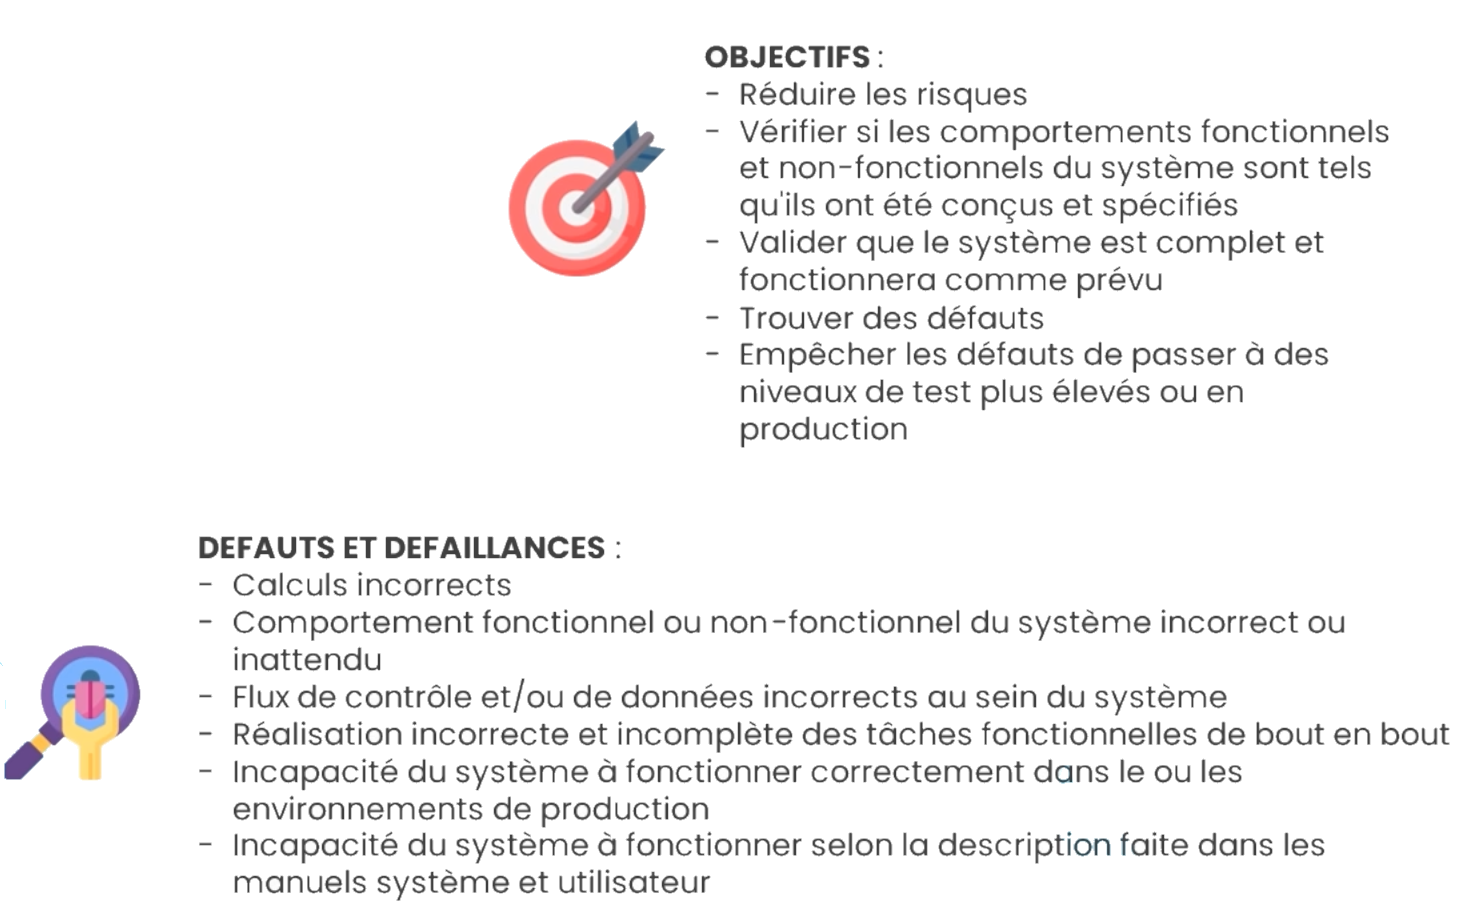
\includegraphics[width=0.9\textwidth]{images/systeme_02.png}
    \end{center}
    
	\subsection{Les tests d'acceptation}

    \begin{center}
        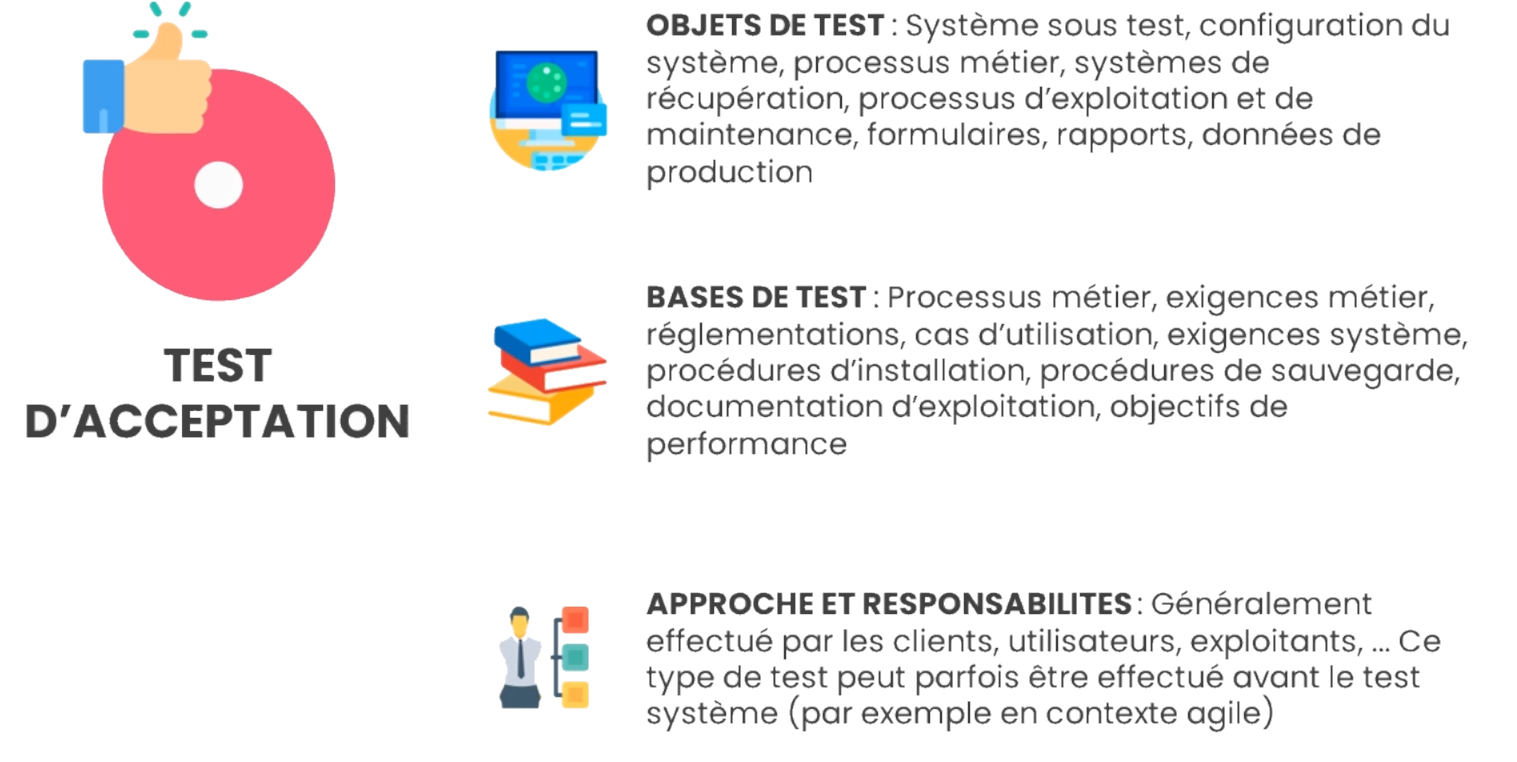
\includegraphics[width=0.9\textwidth]{images/acceptation_01.png}
        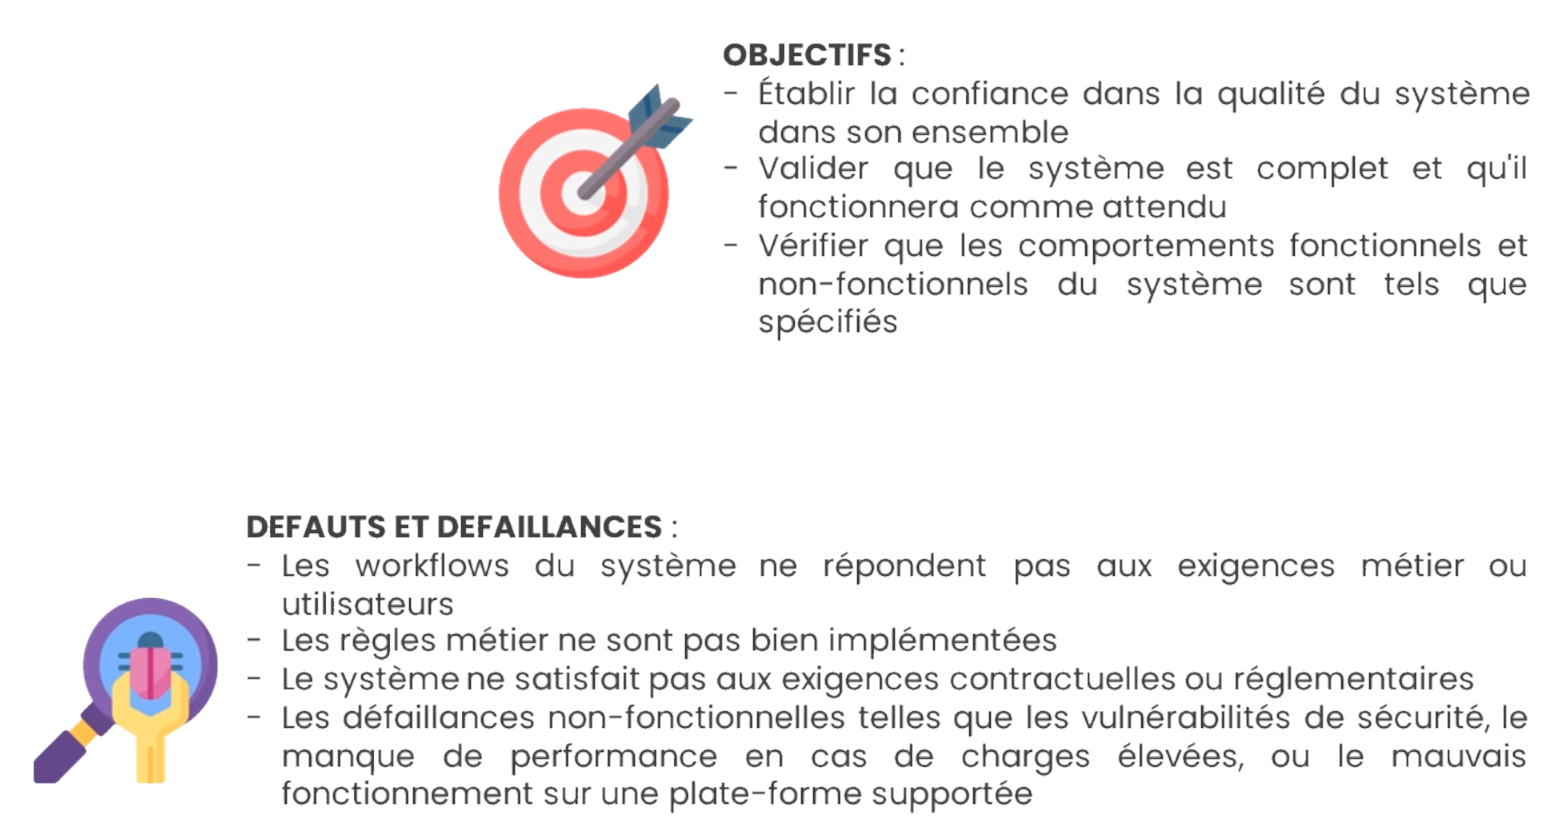
\includegraphics[width=0.9\textwidth]{images/acceptation_02.png}
        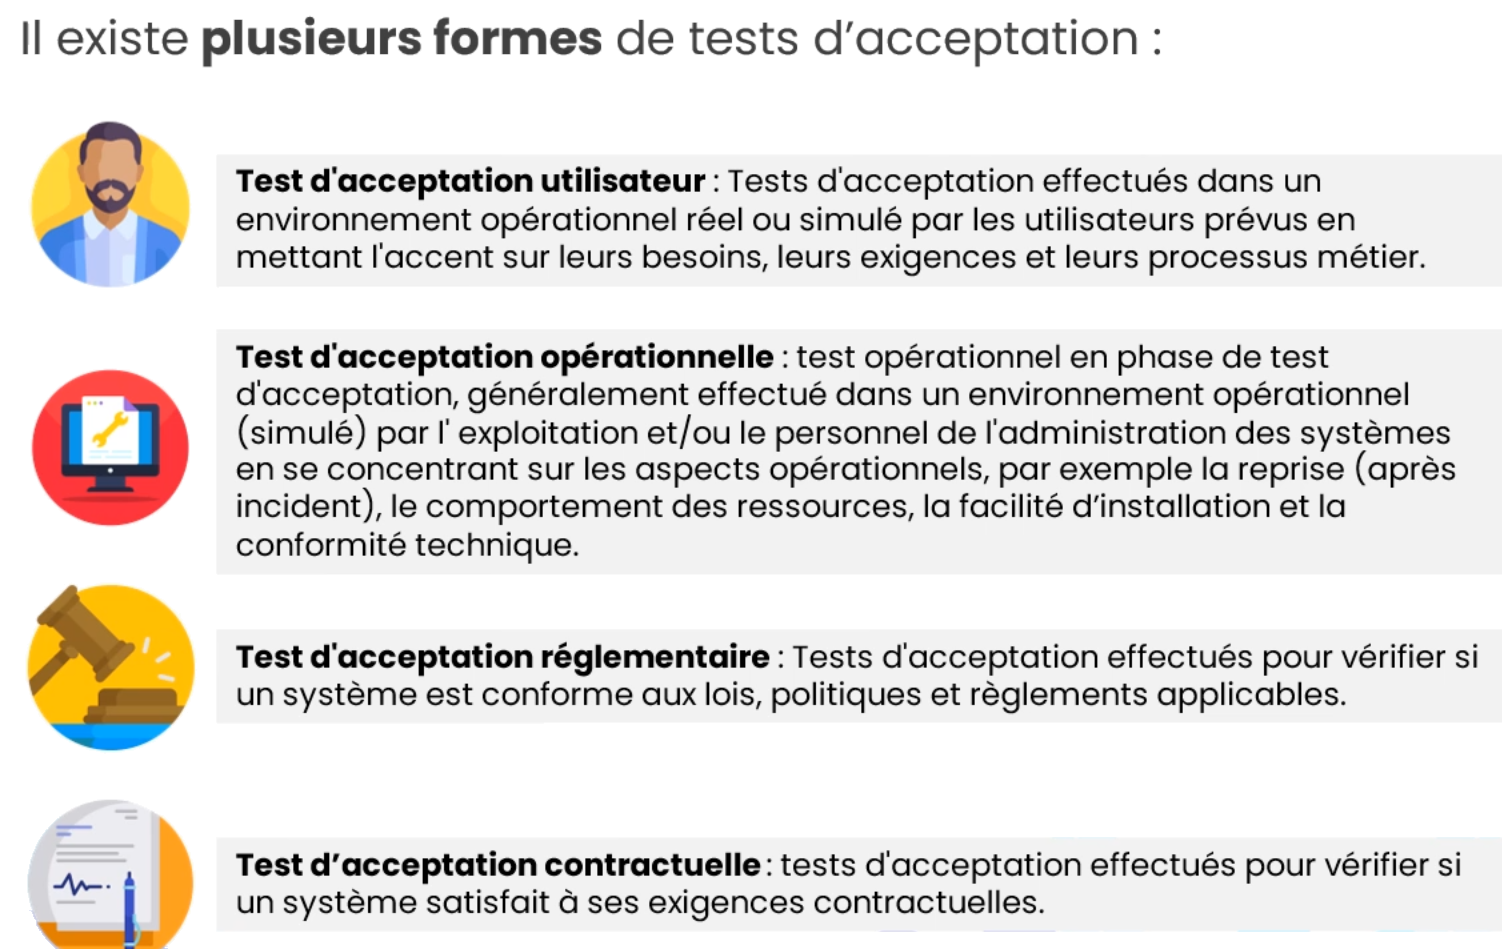
\includegraphics[width=0.9\textwidth]{images/acceptation_03.png}
    \end{center}
    
    \vspace{10mm}
        
    \begin{center}
        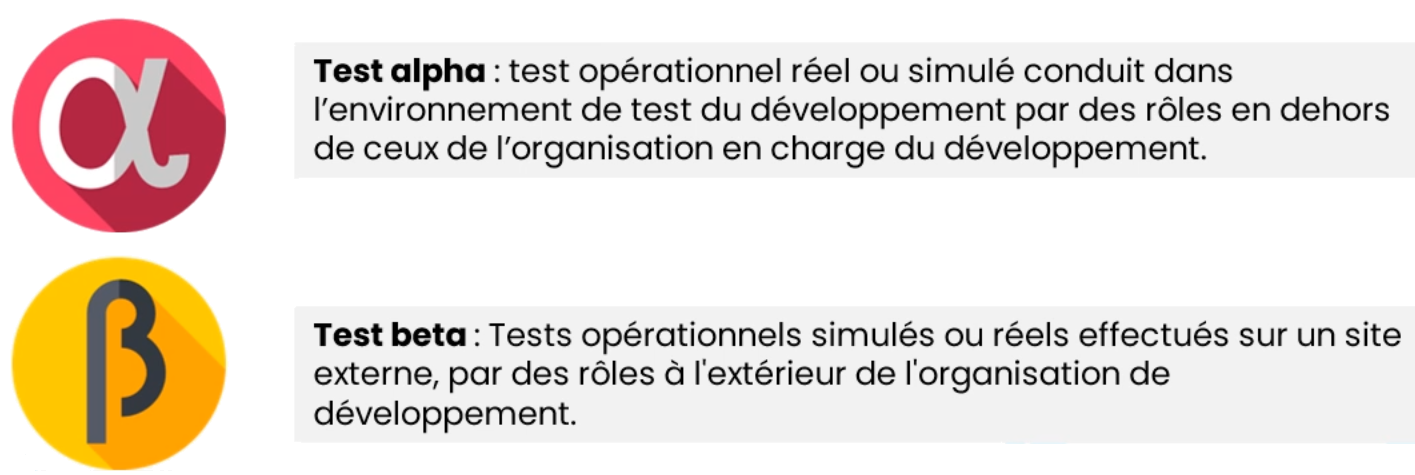
\includegraphics[width=0.9\textwidth]{images/acceptation_04.png}
    \end{center}
    
	\subsection{Les tests fonctionnels et les tests non fonctionnels}

    \begin{center}
        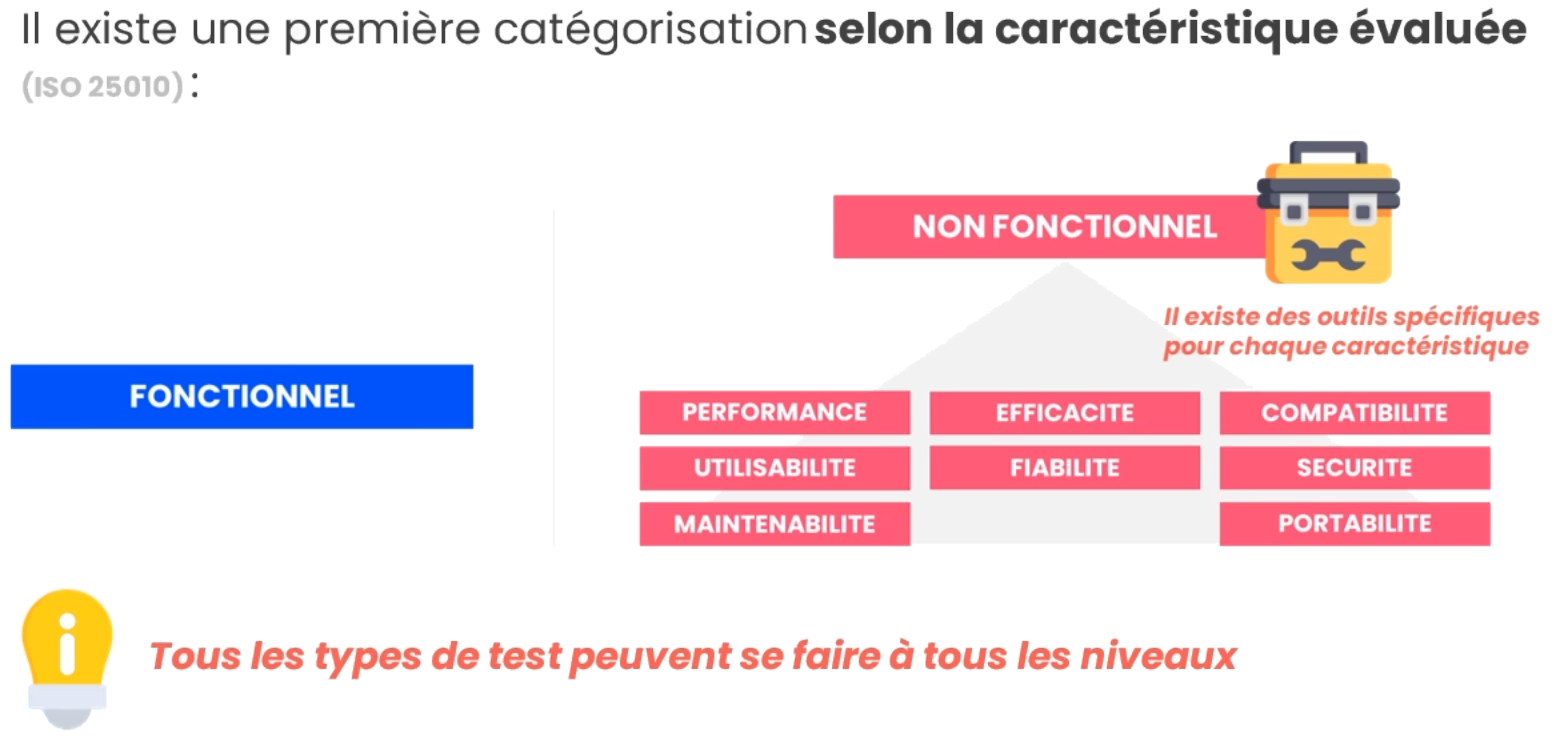
\includegraphics[width=0.9\textwidth]{images/fonc_n_fonc_01.png}
    \end{center}

	 \subsubsection{Les tests fonctionnels}
	  \begin{itemize}
		    	\item Tests unitaires
		    	\item Test de fumée
		    	\item Tests de santé mentale
		    	\item Tests de régression
		    	\item Tests d’intégration
		    	\item Tests d’acceptation par les utilisateurs
		    	\item Test de localisation
		    	\item Test de mondialisation
		    	\item Test du système
		    	\item ...
	  \end{itemize}
	
	
	 \subsubsection{Les tests non fonctionnels}
	  \begin{itemize}
		    	\item Test de charge
		    	\item Tests de résistance
		    	\item Tests de récupération
		    	\item Tests de sécurité
		    	\item Tests d’évolutivité
		    	\item Tests d’endurance
		    	\item Tests de fiabilité
		    	\item Tests de base
		    	\item ...
	  \end{itemize}


    \subsection{Les tests boîte blanche et les tests boîte noire}

    \begin{center}
        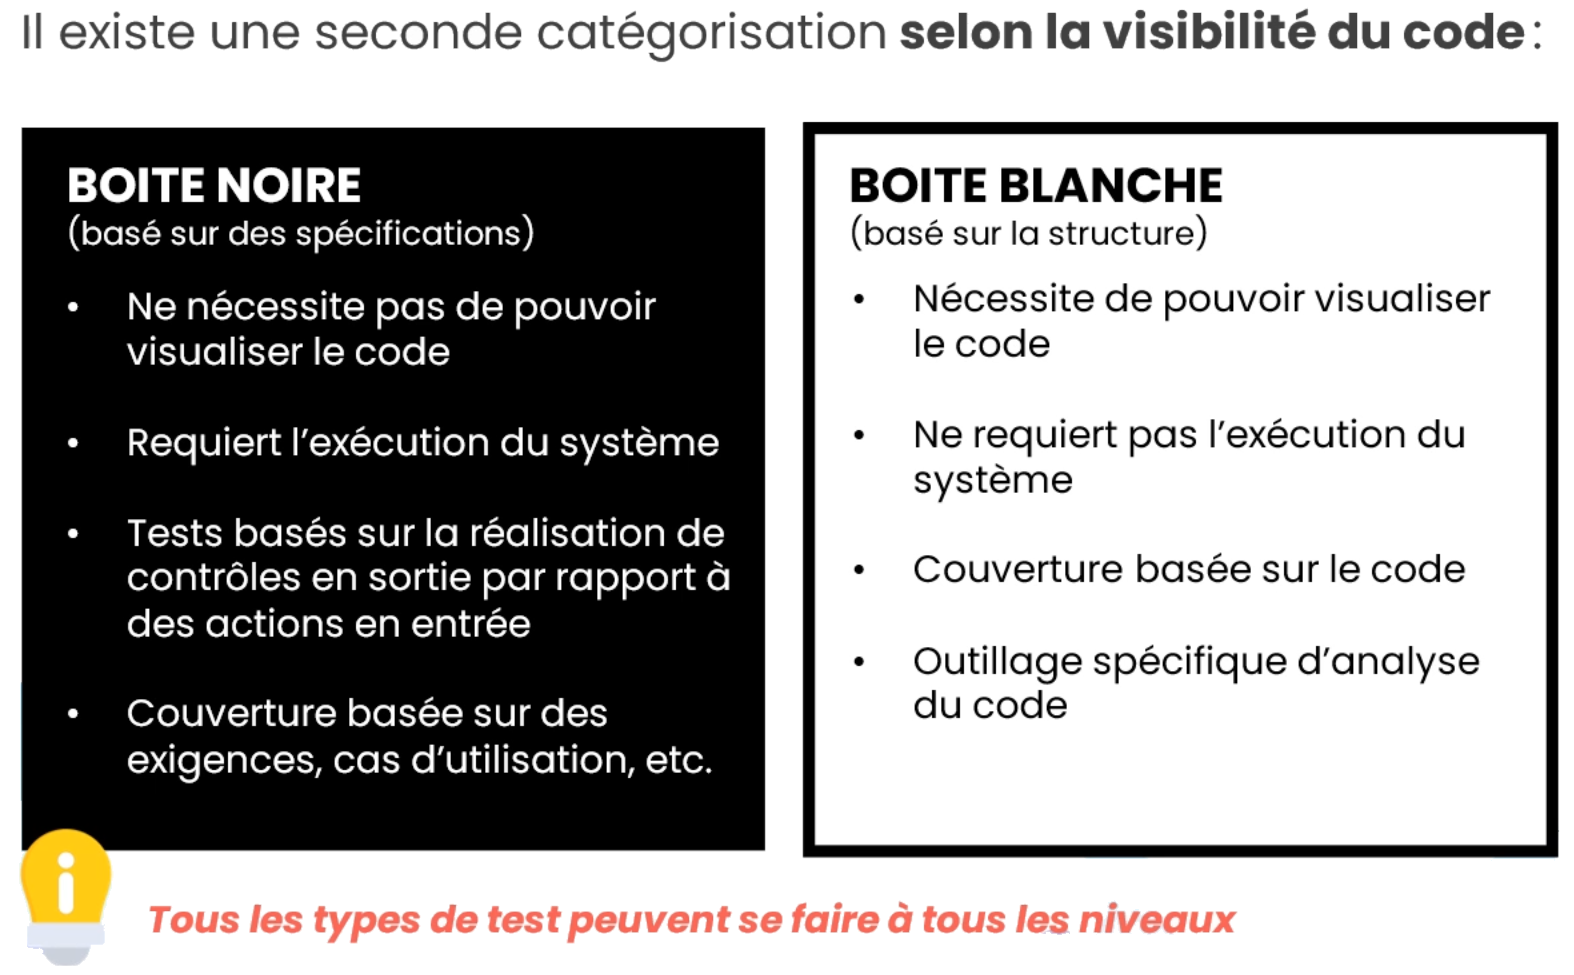
\includegraphics[width=0.9\textwidth]{images/B_N.png}
    \end{center}
    
	\subsection{Les tests de confirmation et les tests de régression}

    \begin{center}
        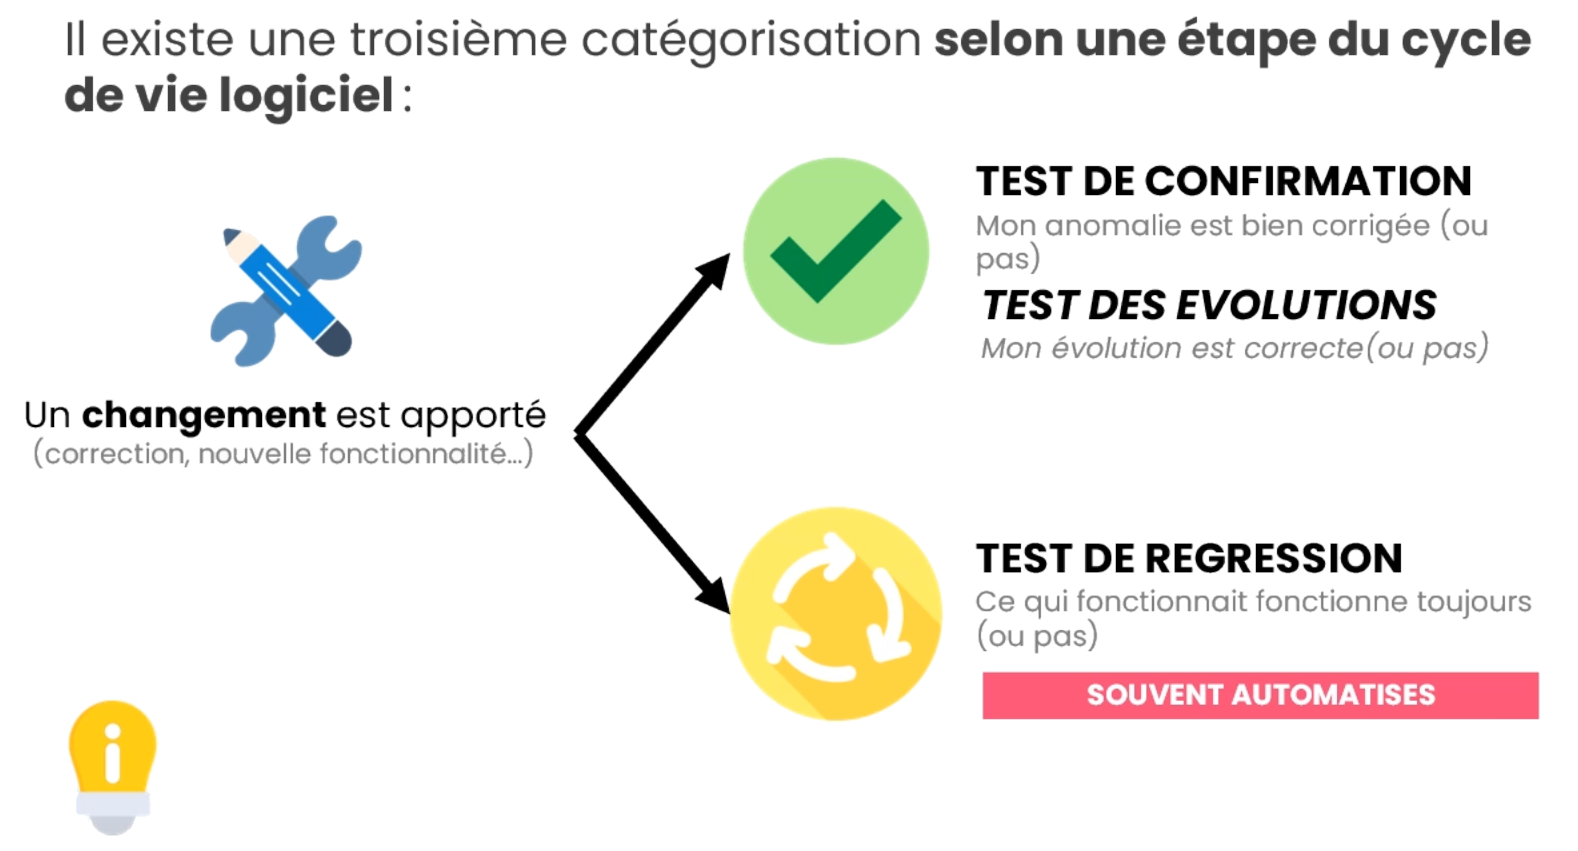
\includegraphics[width=0.9\textwidth]{images/conf_reg.png}
    \end{center}
    
	\subsection{L'environnement de test}

    \begin{center}
        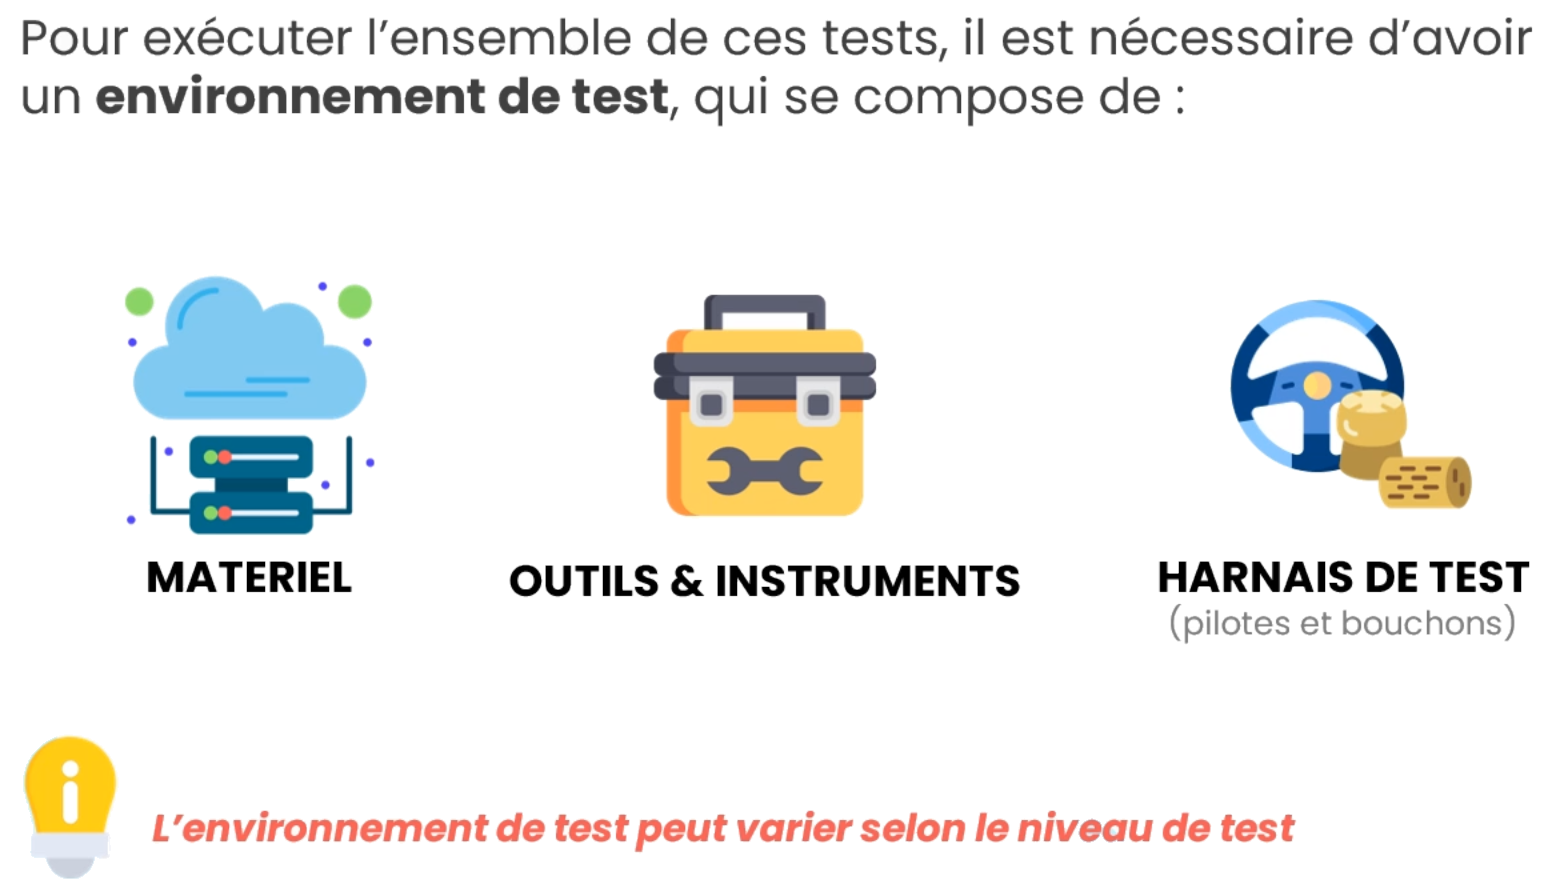
\includegraphics[width=0.9\textwidth]{images/environnement.png}
    \end{center}
    
	\subsection{Les tests de maintenance}

    \begin{center}
        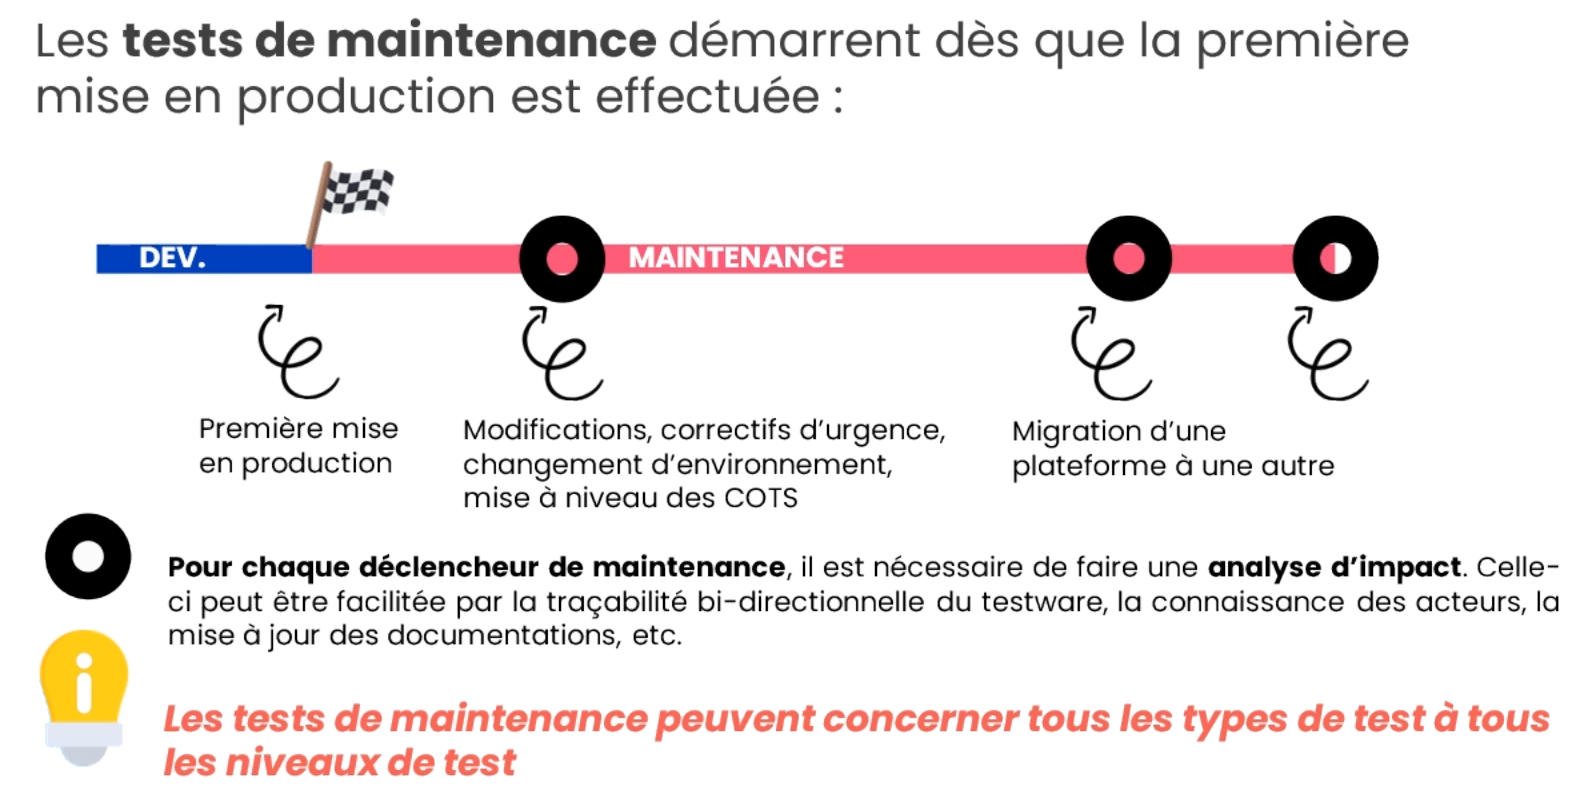
\includegraphics[width=0.9\textwidth]{images/maintenance.png}
    \end{center}


\pagebreak
\section{TESTS STATIQUES}

	\subsection{Les tests statiques vs tests dynamiques}

    \begin{center}
        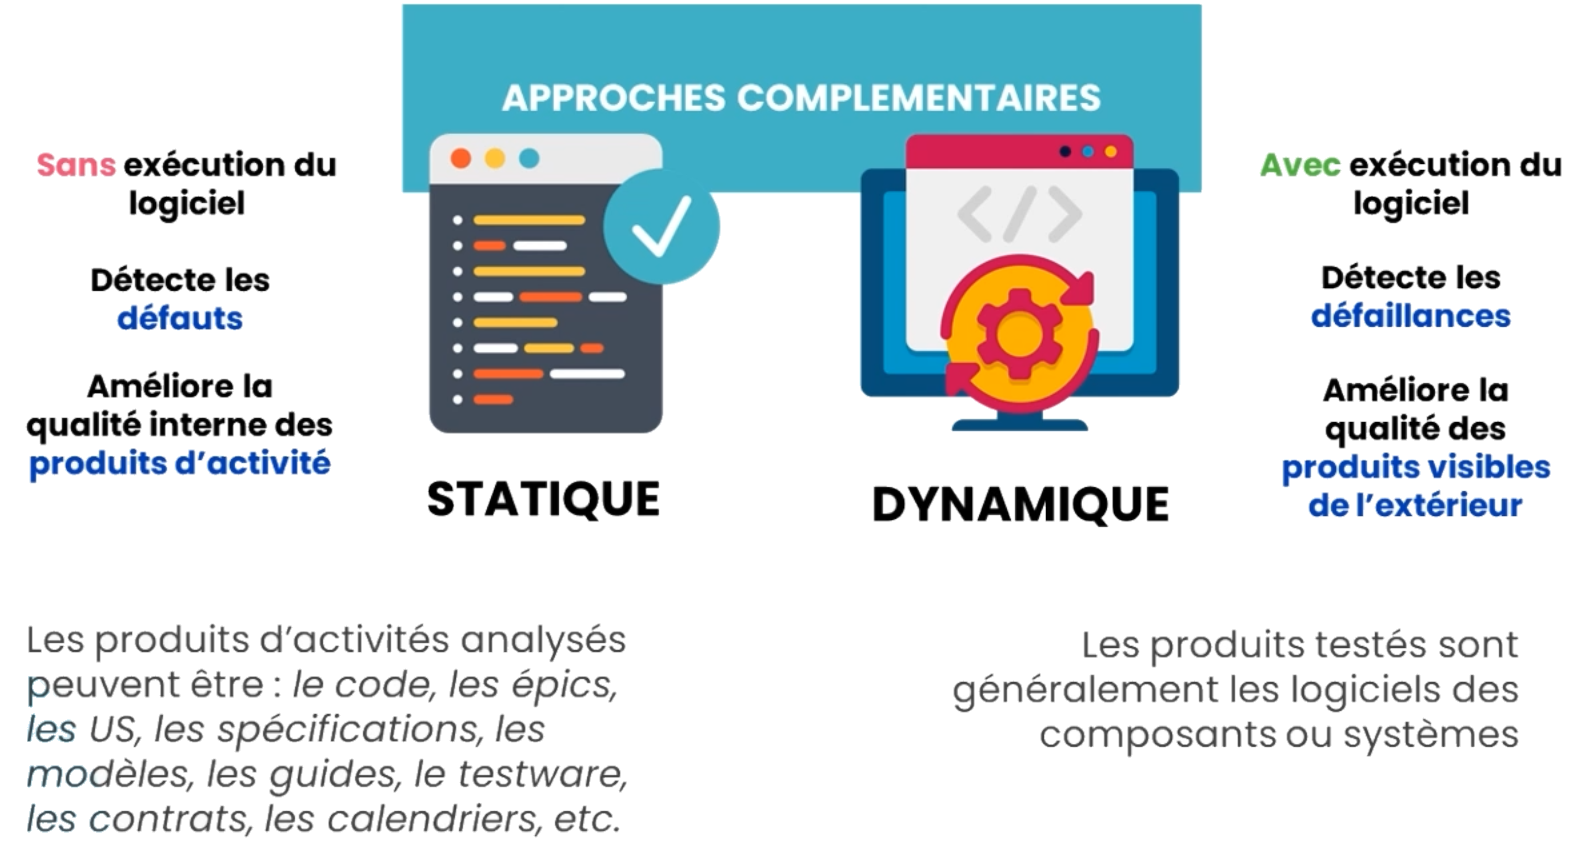
\includegraphics[width=0.9\textwidth]{images/stat_vs_dyn_01.png}
    \end{center}
    
	\subsection{Les avantages des tests statiques}

    \begin{center}
        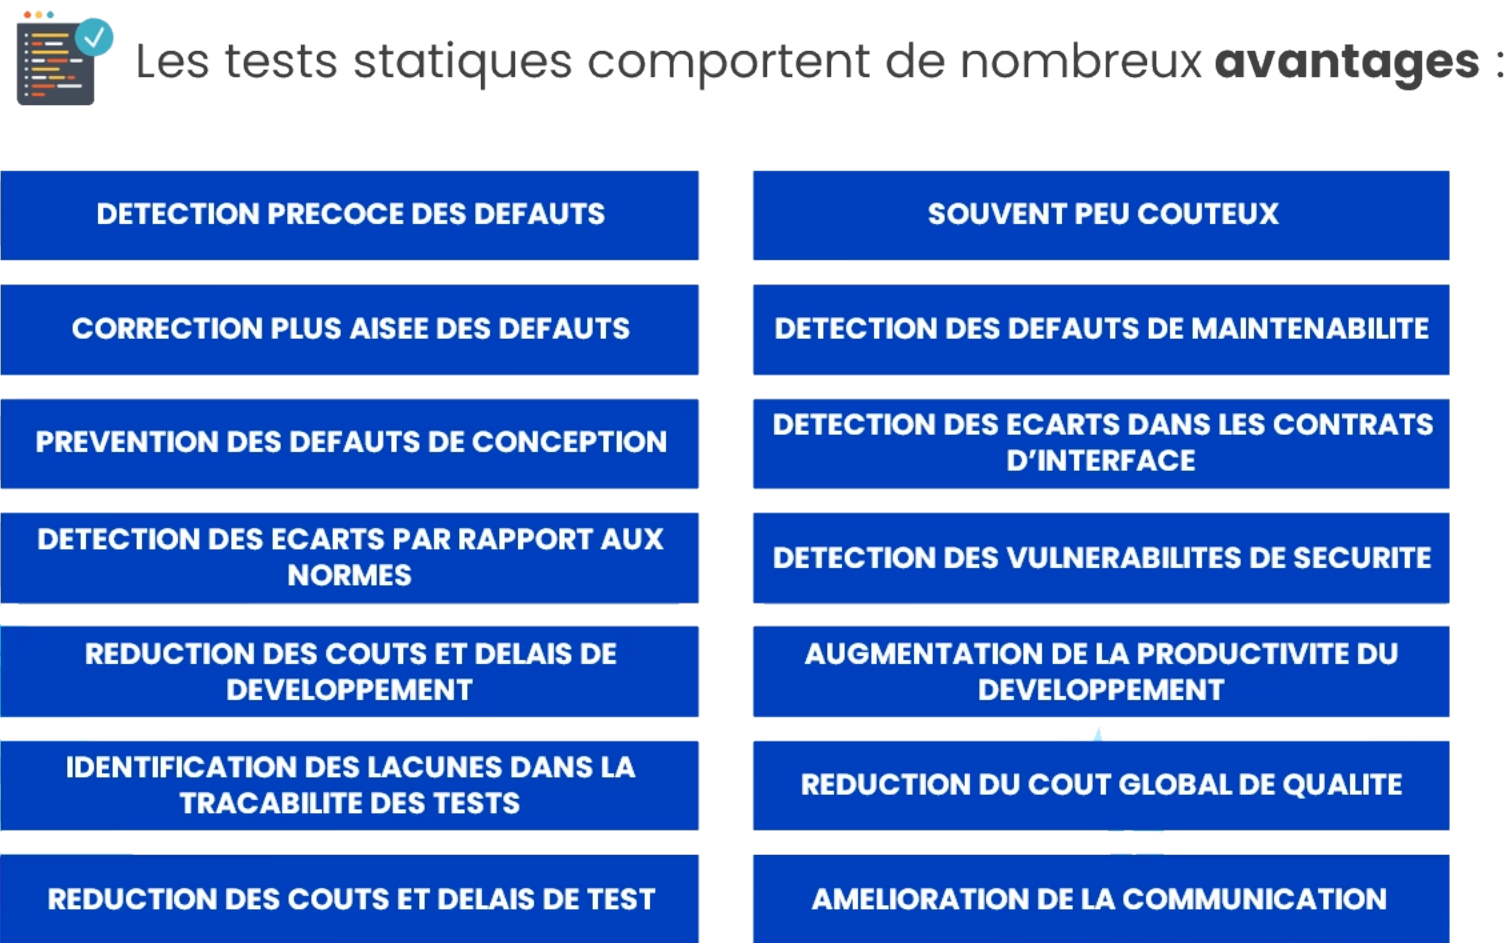
\includegraphics[width=0.9\textwidth]{images/stat_vs_dyn_02.png}
    \end{center}
    
	\subsection{La revue d'analyse statique}

    \begin{center}
        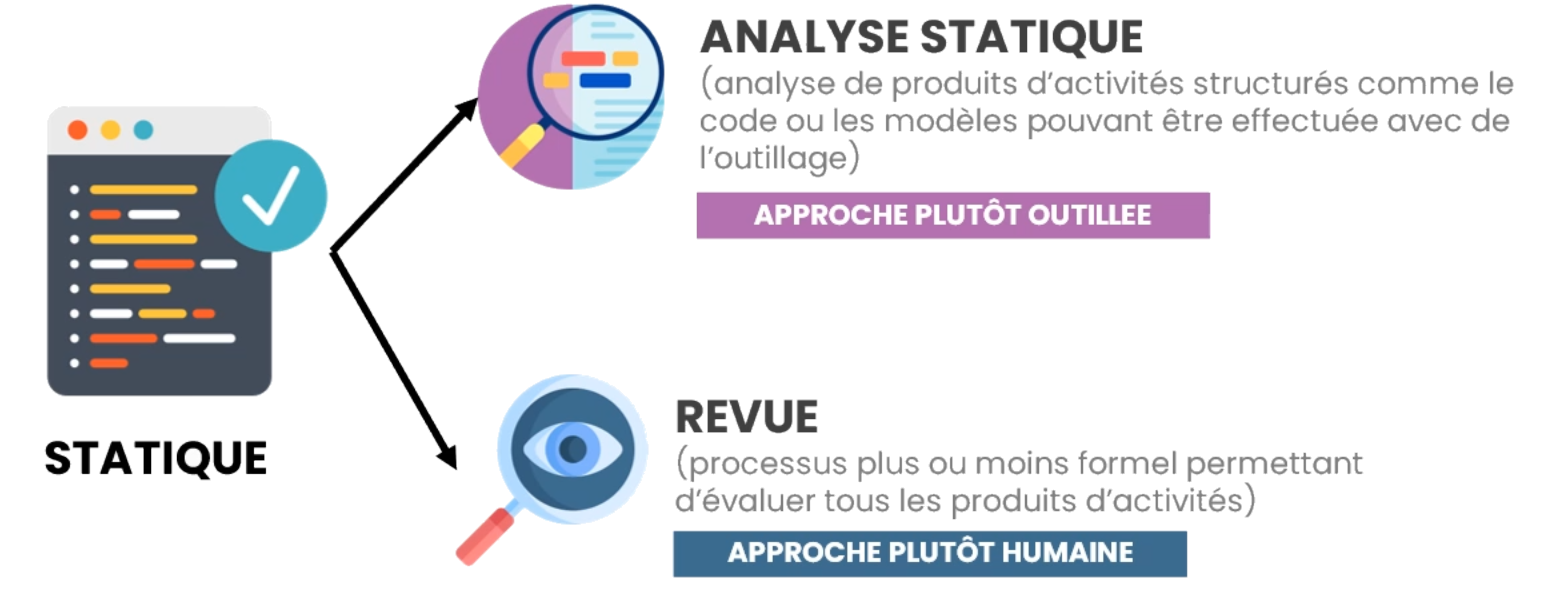
\includegraphics[width=0.9\textwidth]{images/stat.png}
    \end{center}
    
	\subsection{Les types de revue}
    
    \begin{center}
        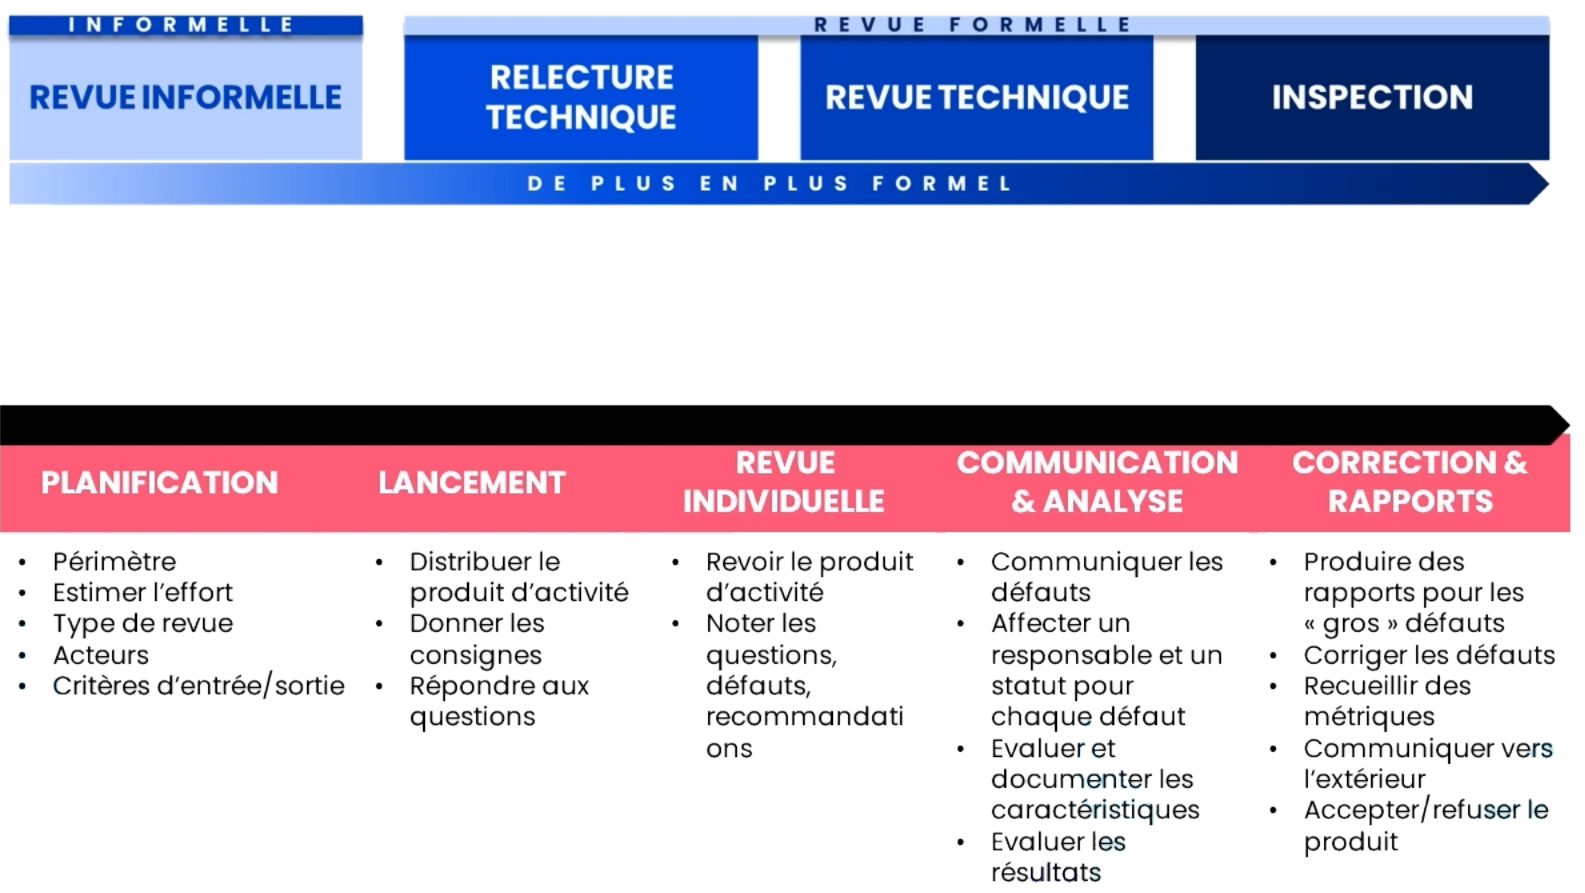
\includegraphics[width=0.9\textwidth]{images/revues.png}
    \end{center}
    
	\subsection{Les rôles}

    \begin{center}
        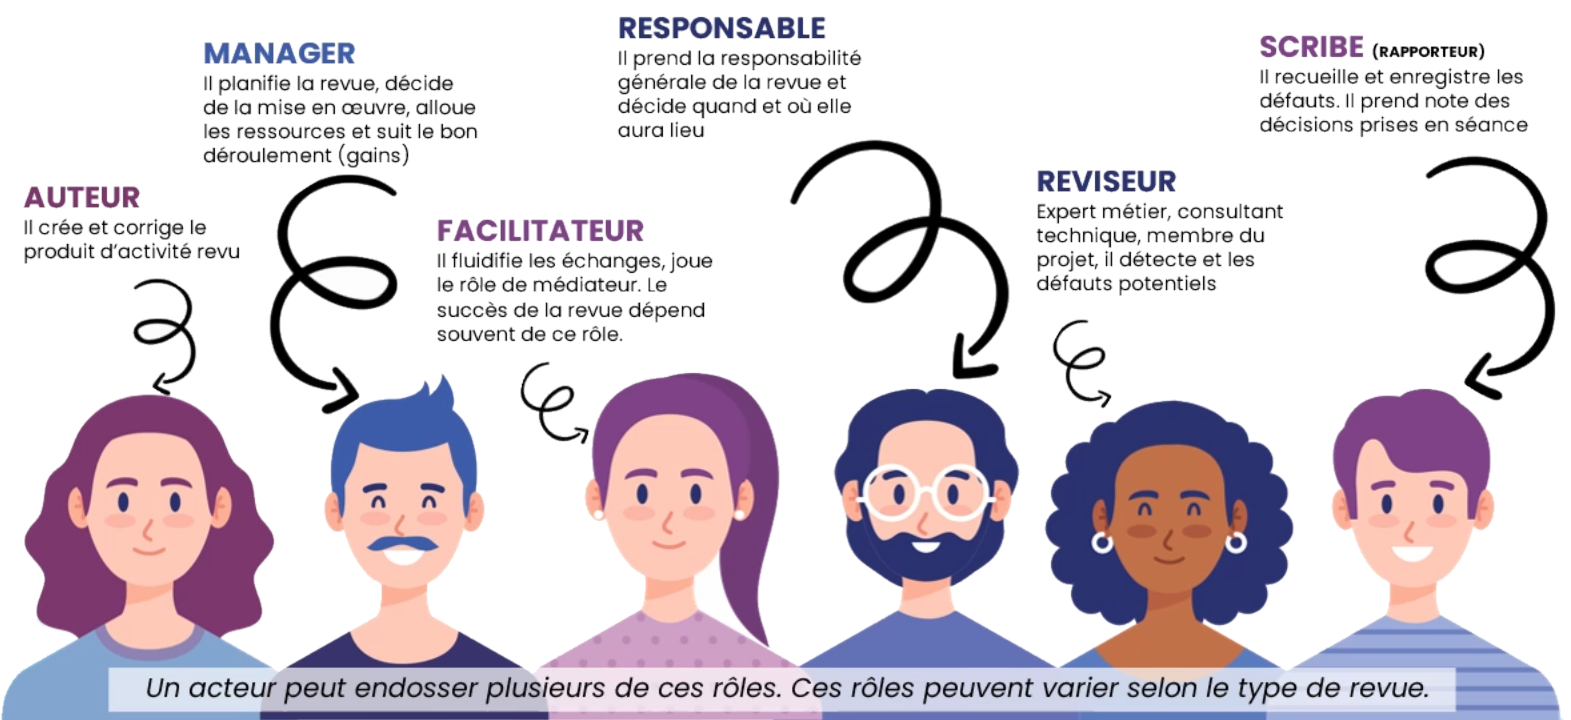
\includegraphics[width=0.9\textwidth]{images/roles.png}
    \end{center}
    
	\subsection{La revue informelle}

    \begin{center}
        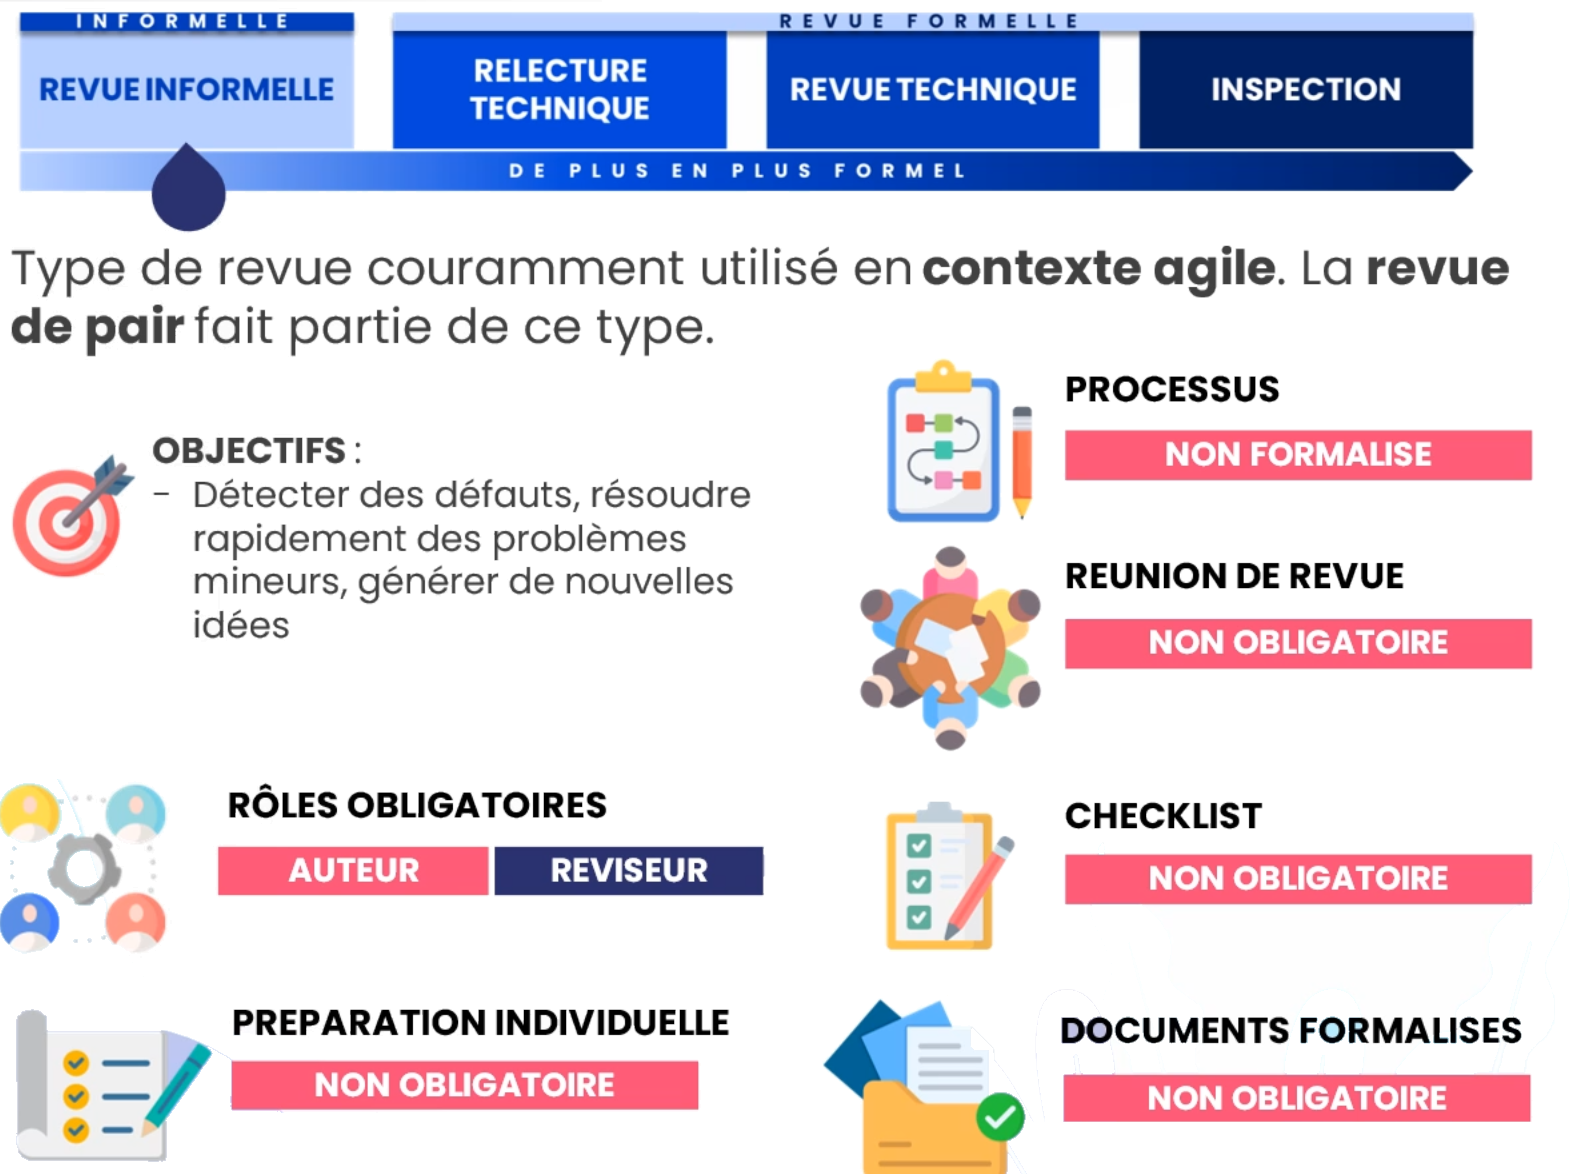
\includegraphics[width=0.9\textwidth]{images/informelle.png}
    \end{center}
    
	\subsection{La relecture technique}

    \begin{center}
        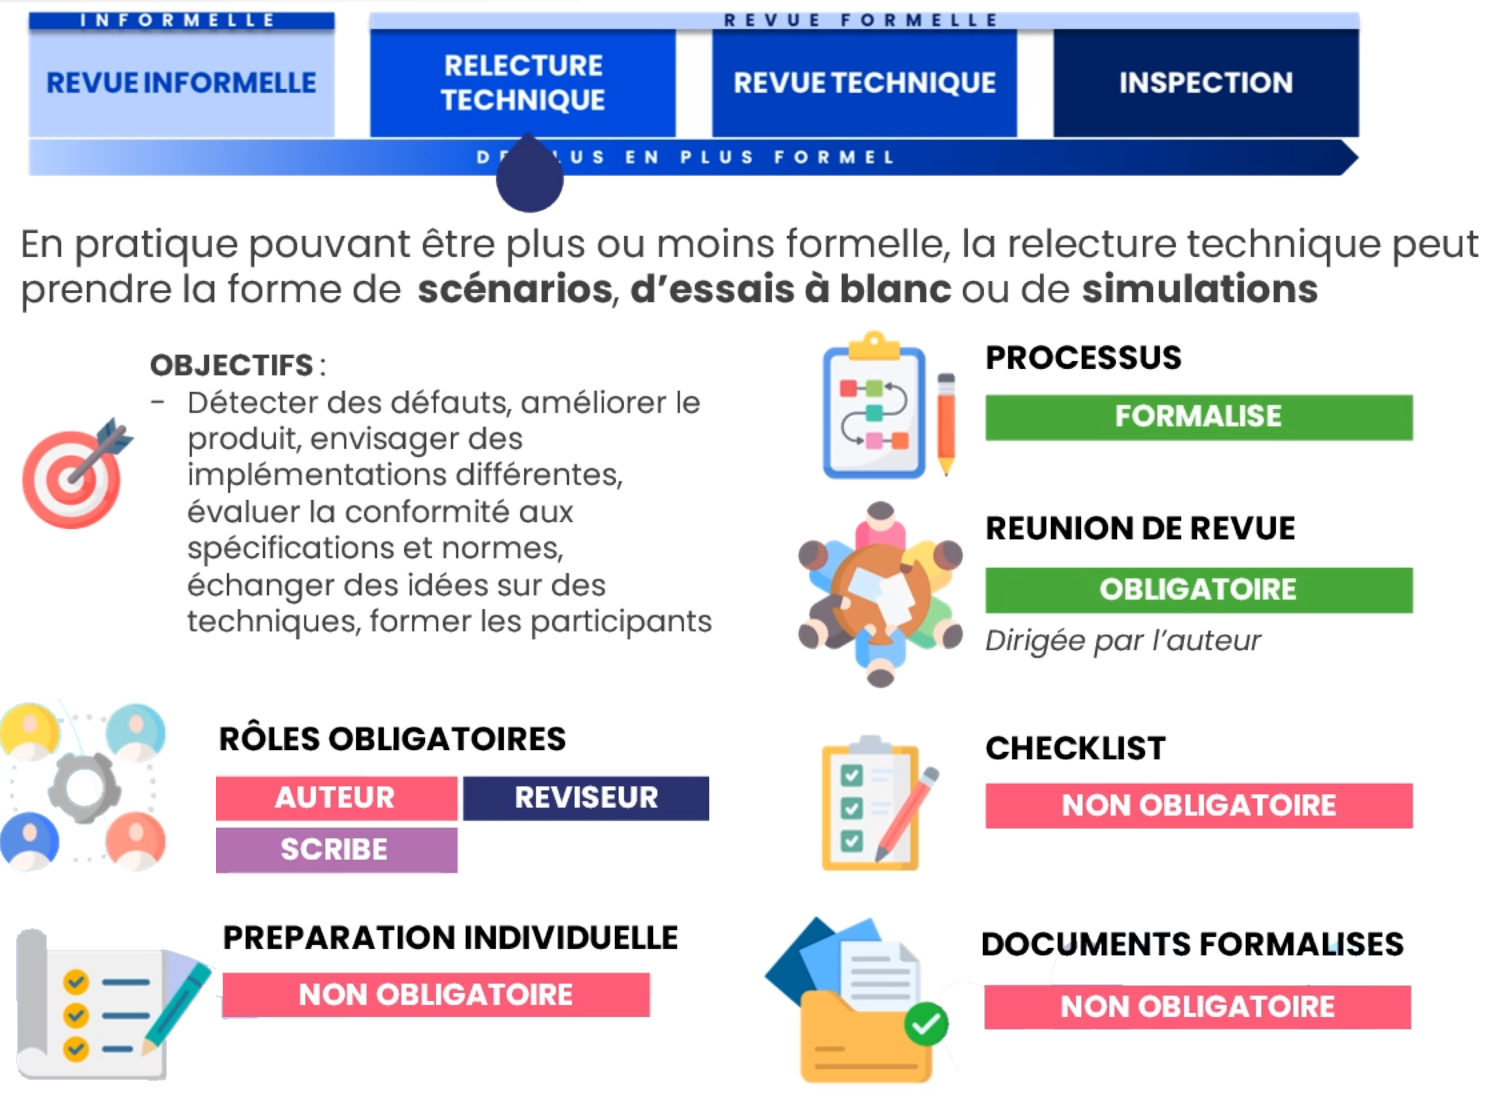
\includegraphics[width=0.9\textwidth]{images/tech_01.png}
    \end{center}
    
	\subsection{La revue technique}

    \begin{center}
        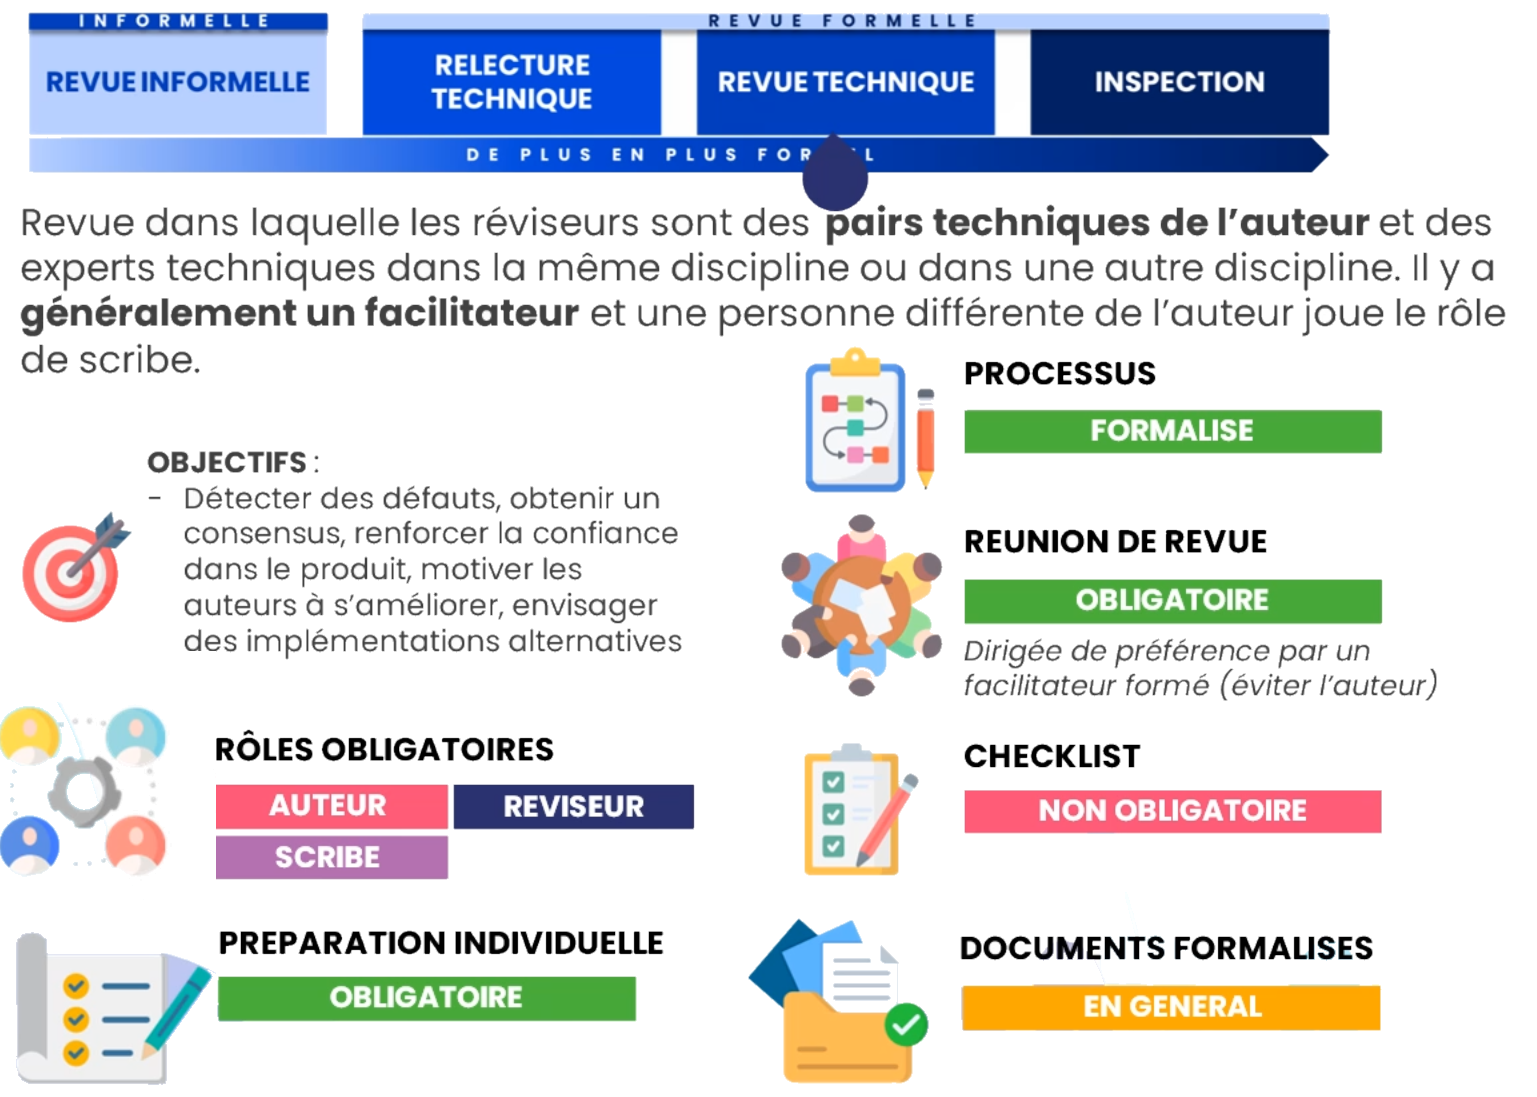
\includegraphics[width=0.9\textwidth]{images/tech_02.png}
    \end{center}
    
	\subsection{L'inspection}

    \begin{center}
        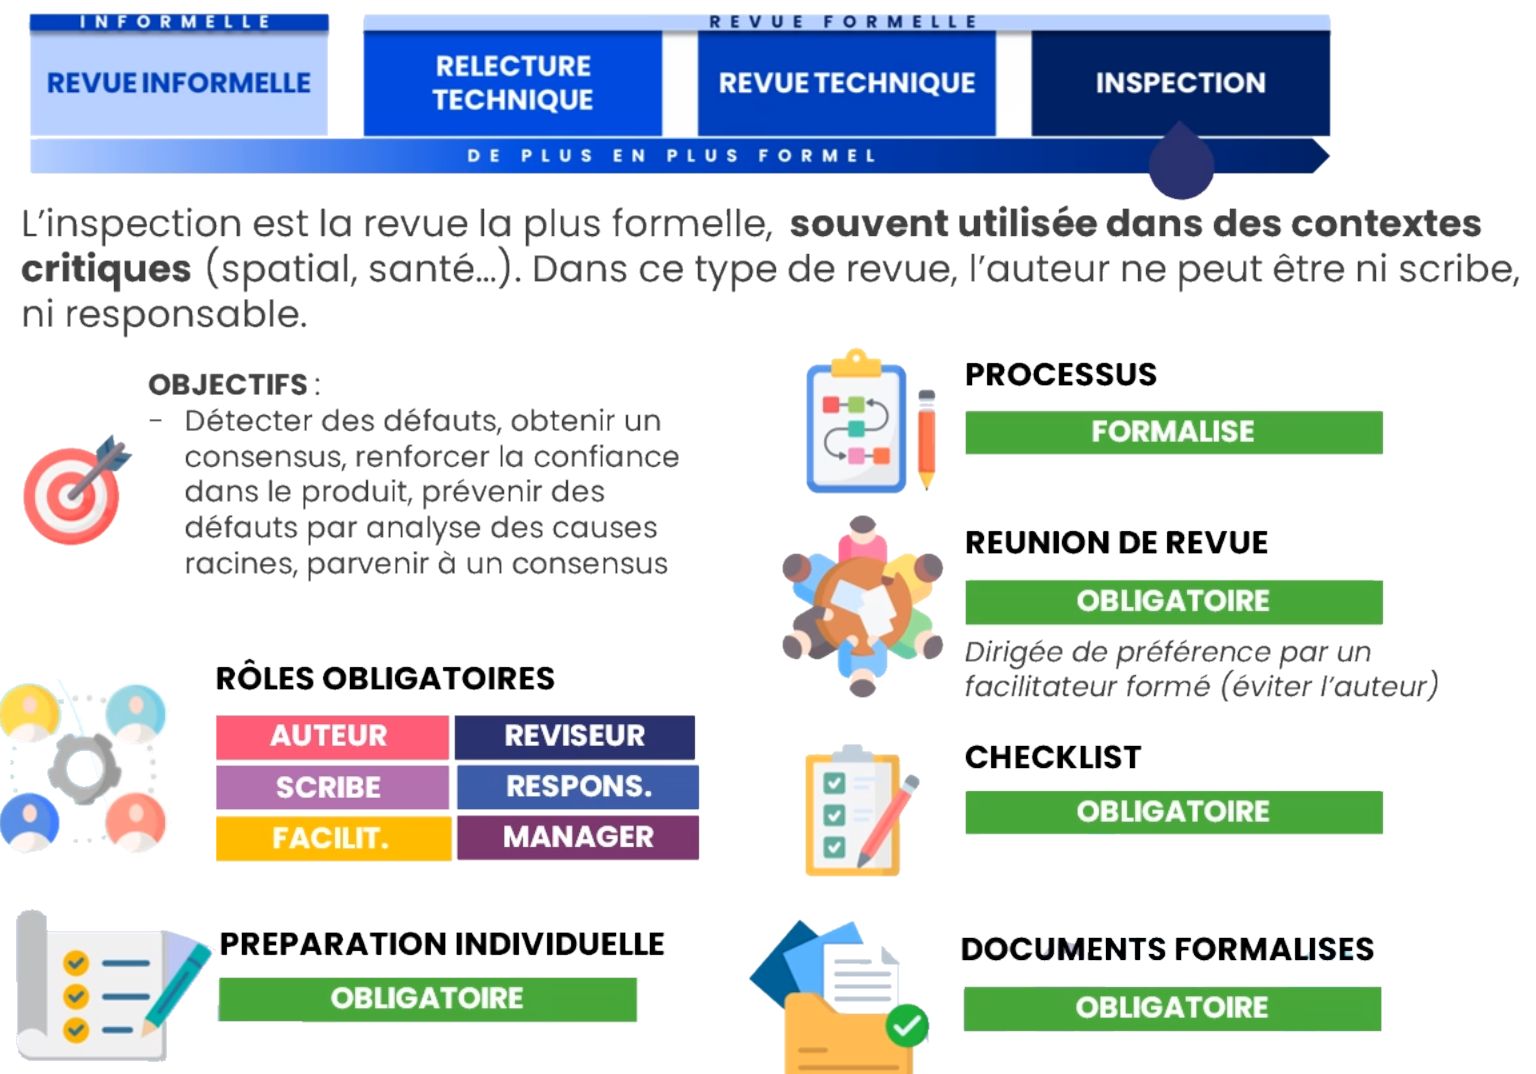
\includegraphics[width=0.9\textwidth]{images/inspection.png}
    \end{center}
    
	\subsection{Les techniques de revue}

    \begin{center}
        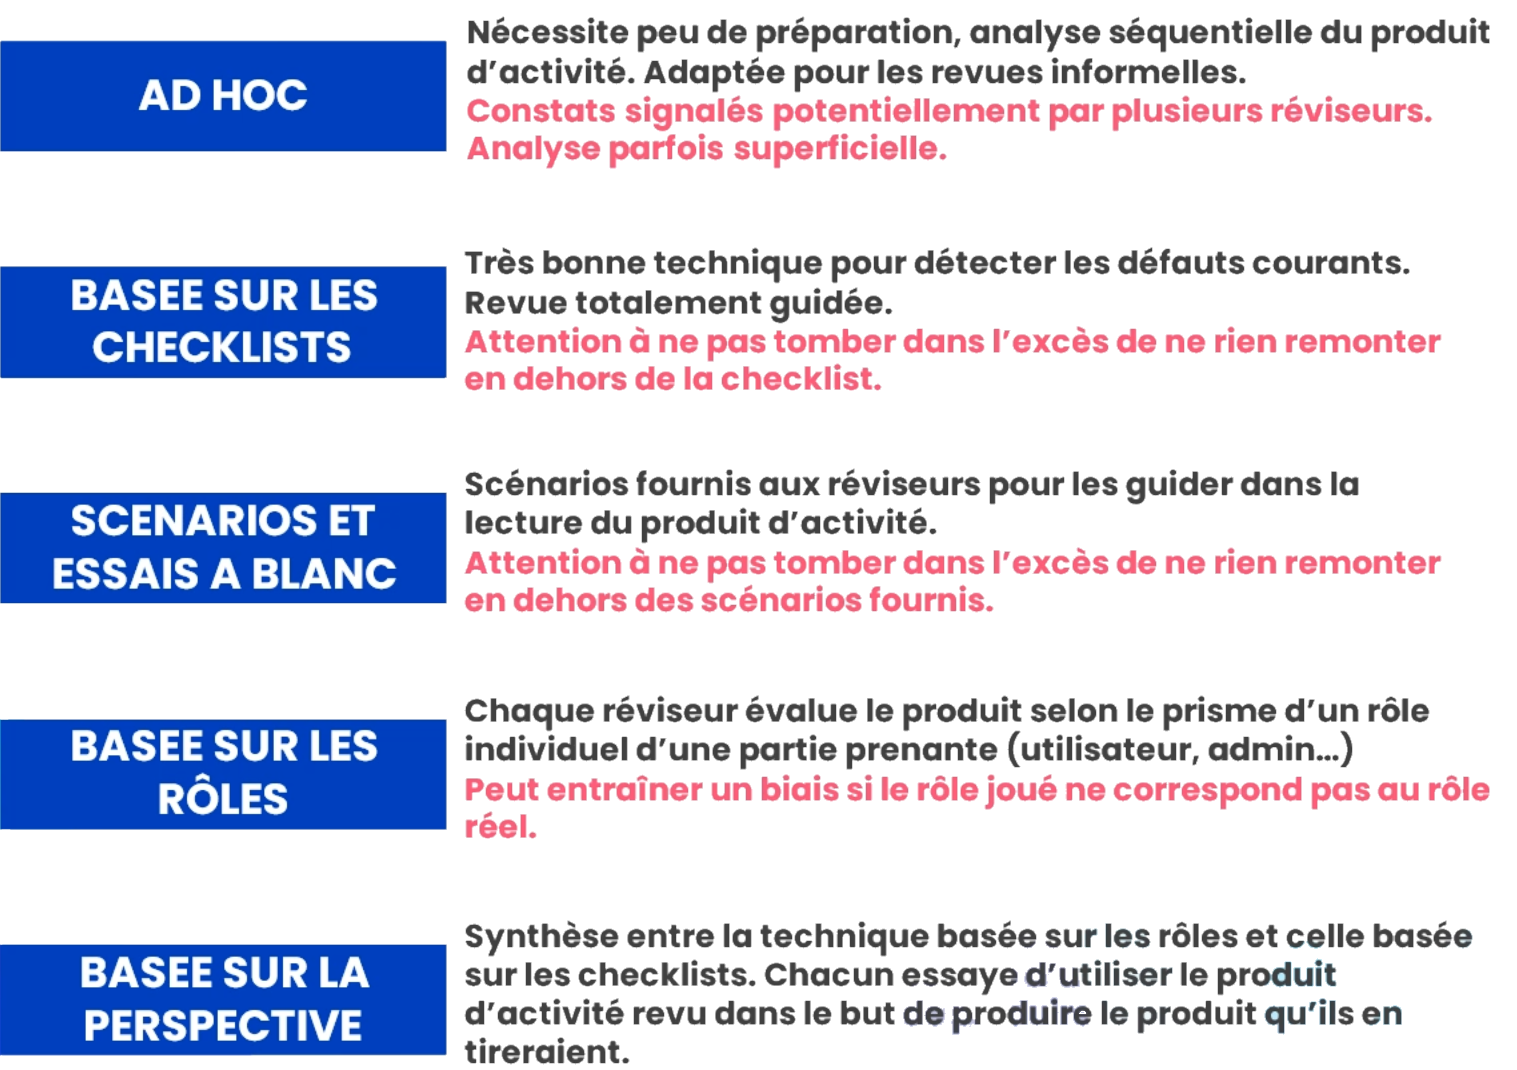
\includegraphics[width=0.9\textwidth]{images/tech_revue.png}
    \end{center}
    
	\subsection{Les facteurs de succès}

    \begin{center}
        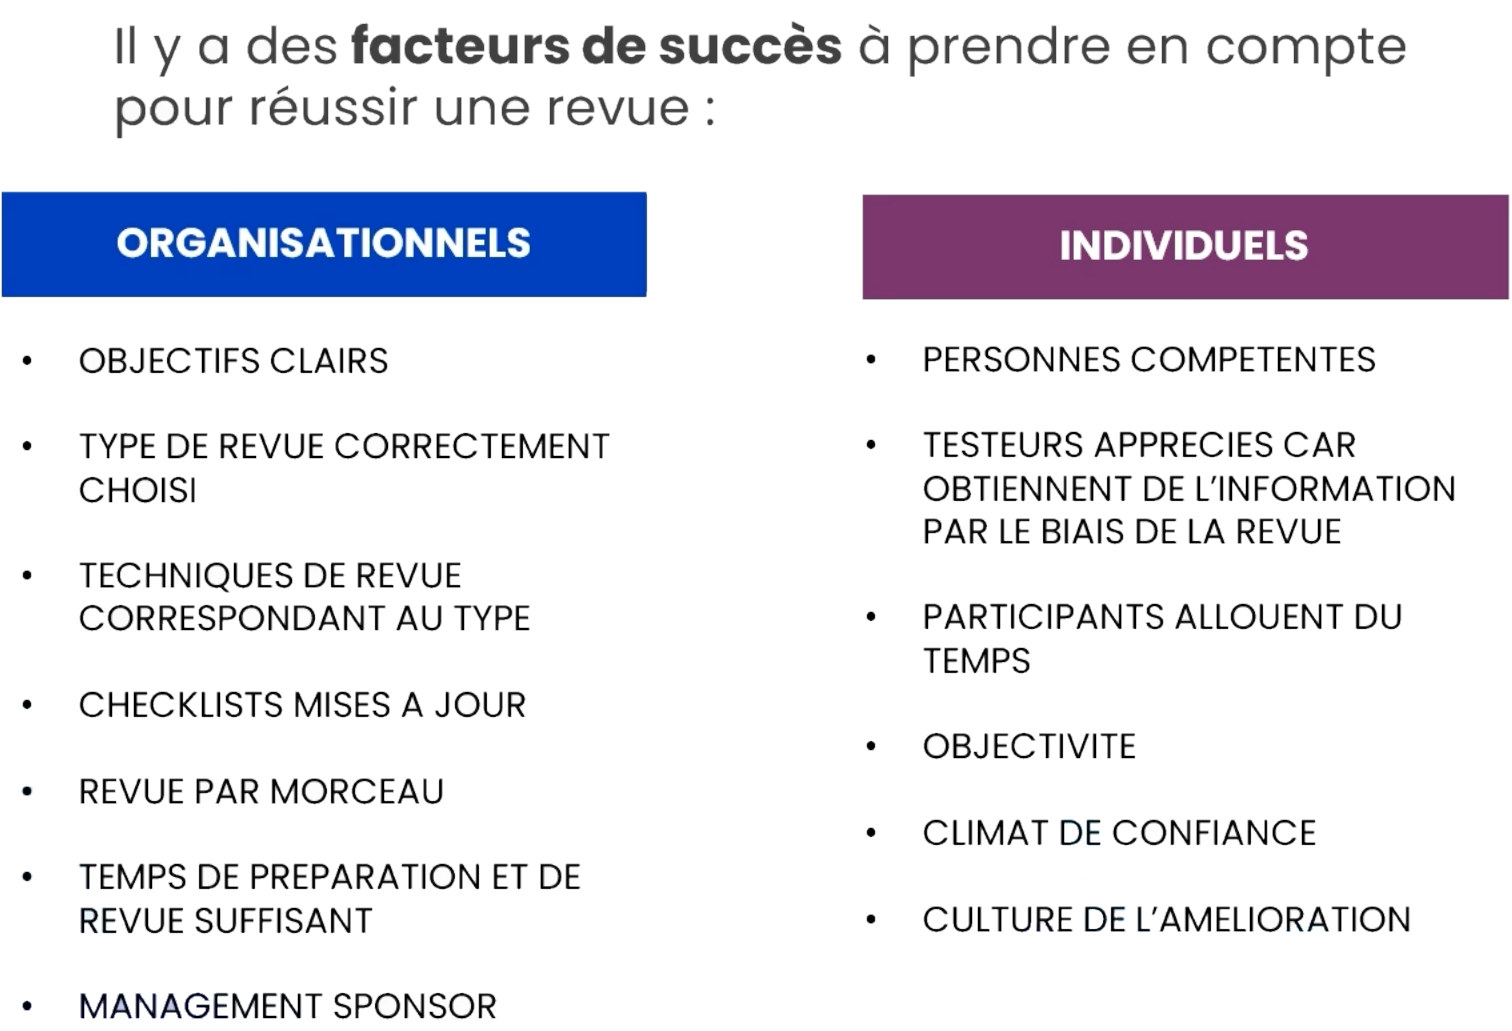
\includegraphics[width=0.9\textwidth]{images/fact.png}
    \end{center}
    
	% \subsection{Exercice Et Conclusion}


\pagebreak
\section{TECHNIQUES D'ANALYSE ET DE CONCEPTION DES TESTS}

	\subsection{Les techniques}

    \begin{center}
        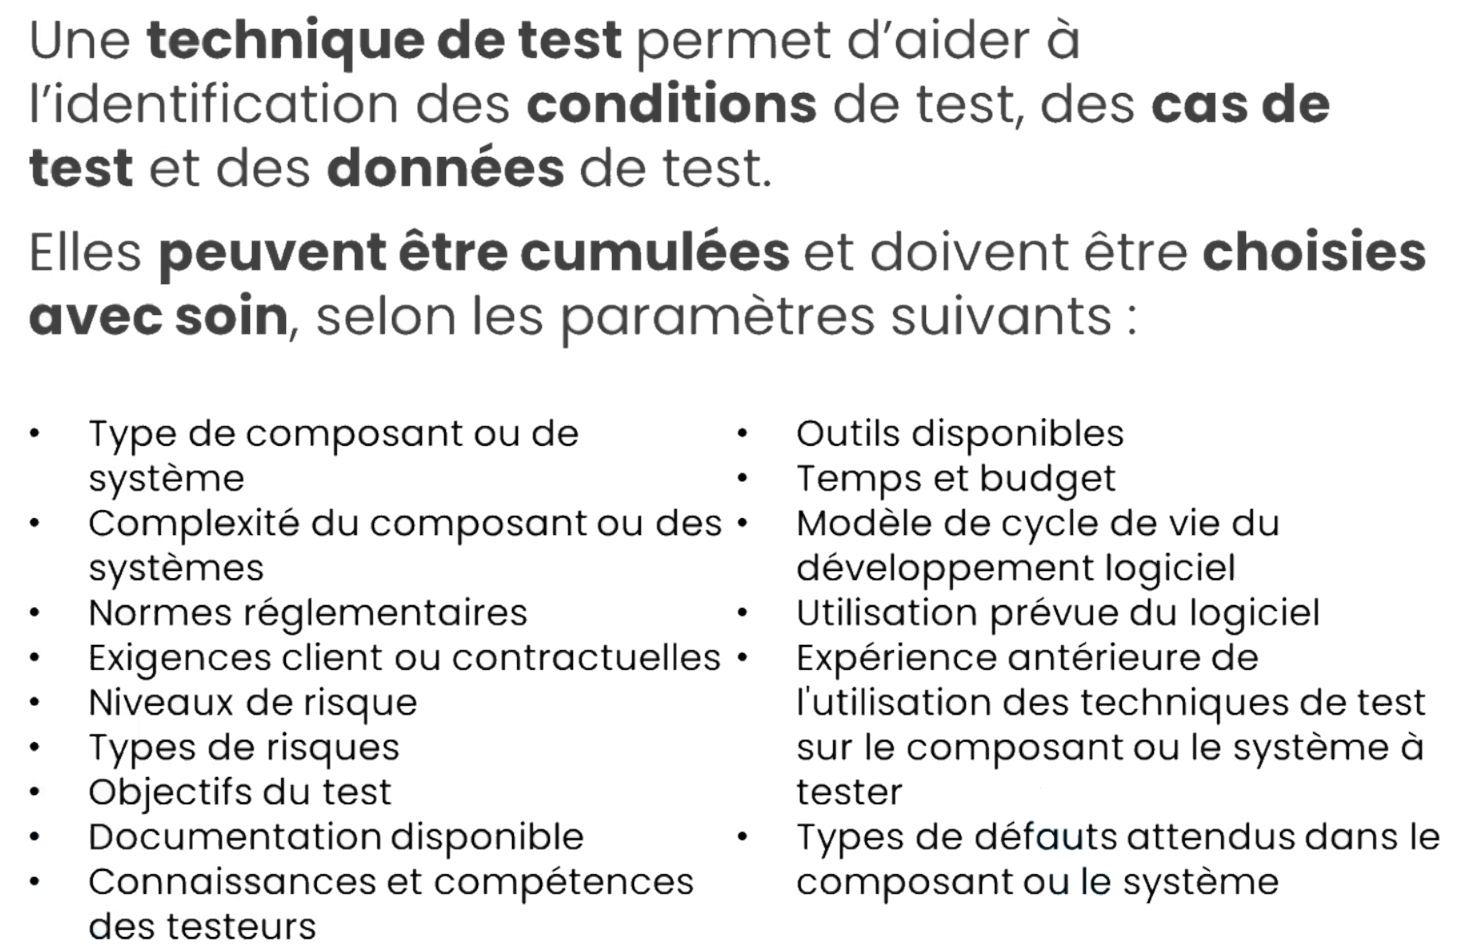
\includegraphics[width=0.9\textwidth]{images/tech_test_01.png}
    \end{center}
    
    \subsubsection{Techniques boîte noire \& boite blanche}
    
    \begin{center}
    	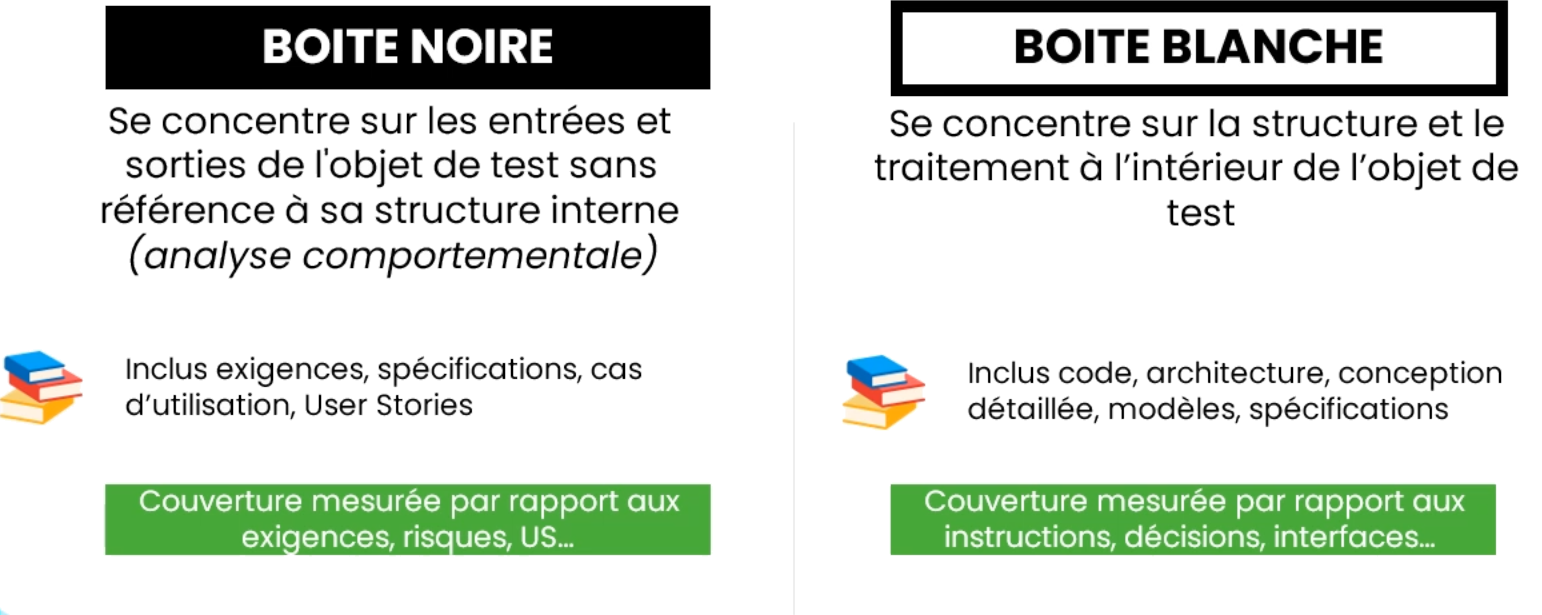
\includegraphics[width=0.9\textwidth]{images/tech_test_02.png}
    \end{center}
    
    \subsubsection{Techniques Expérience \& Collaboration}
    
    \begin{center}
    	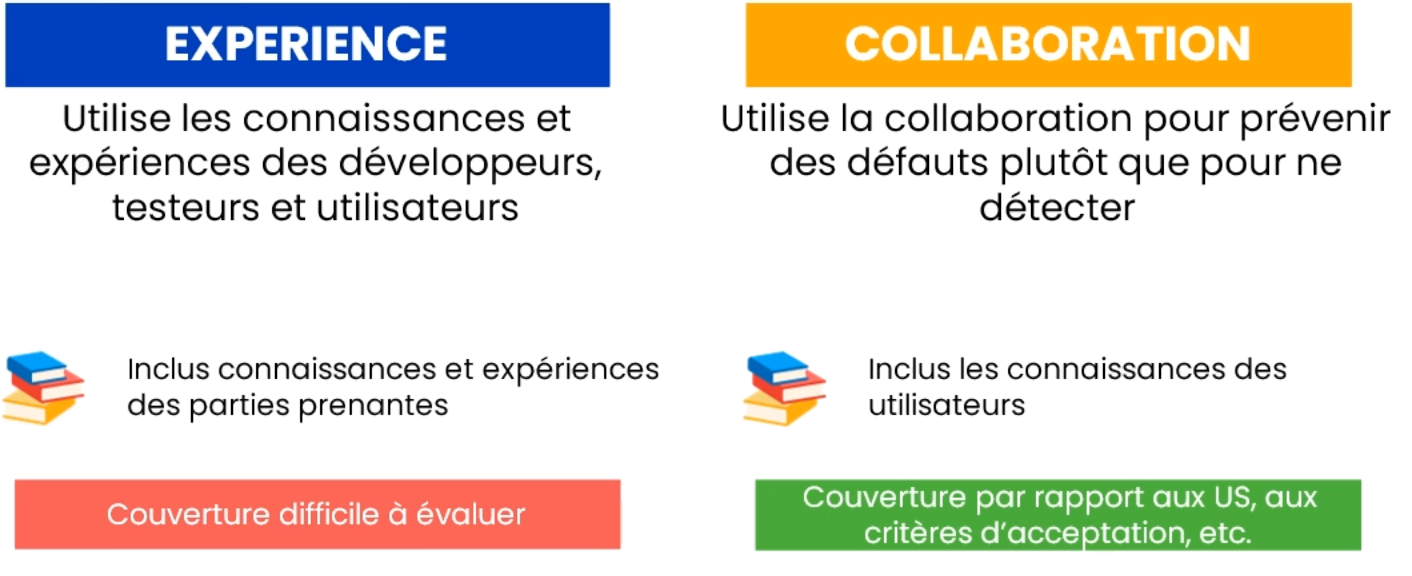
\includegraphics[width=0.9\textwidth]{images/tech_test_03.png}
    \end{center}
    
	\subsection{La technique de partitions / équivalence}

    \begin{center}
        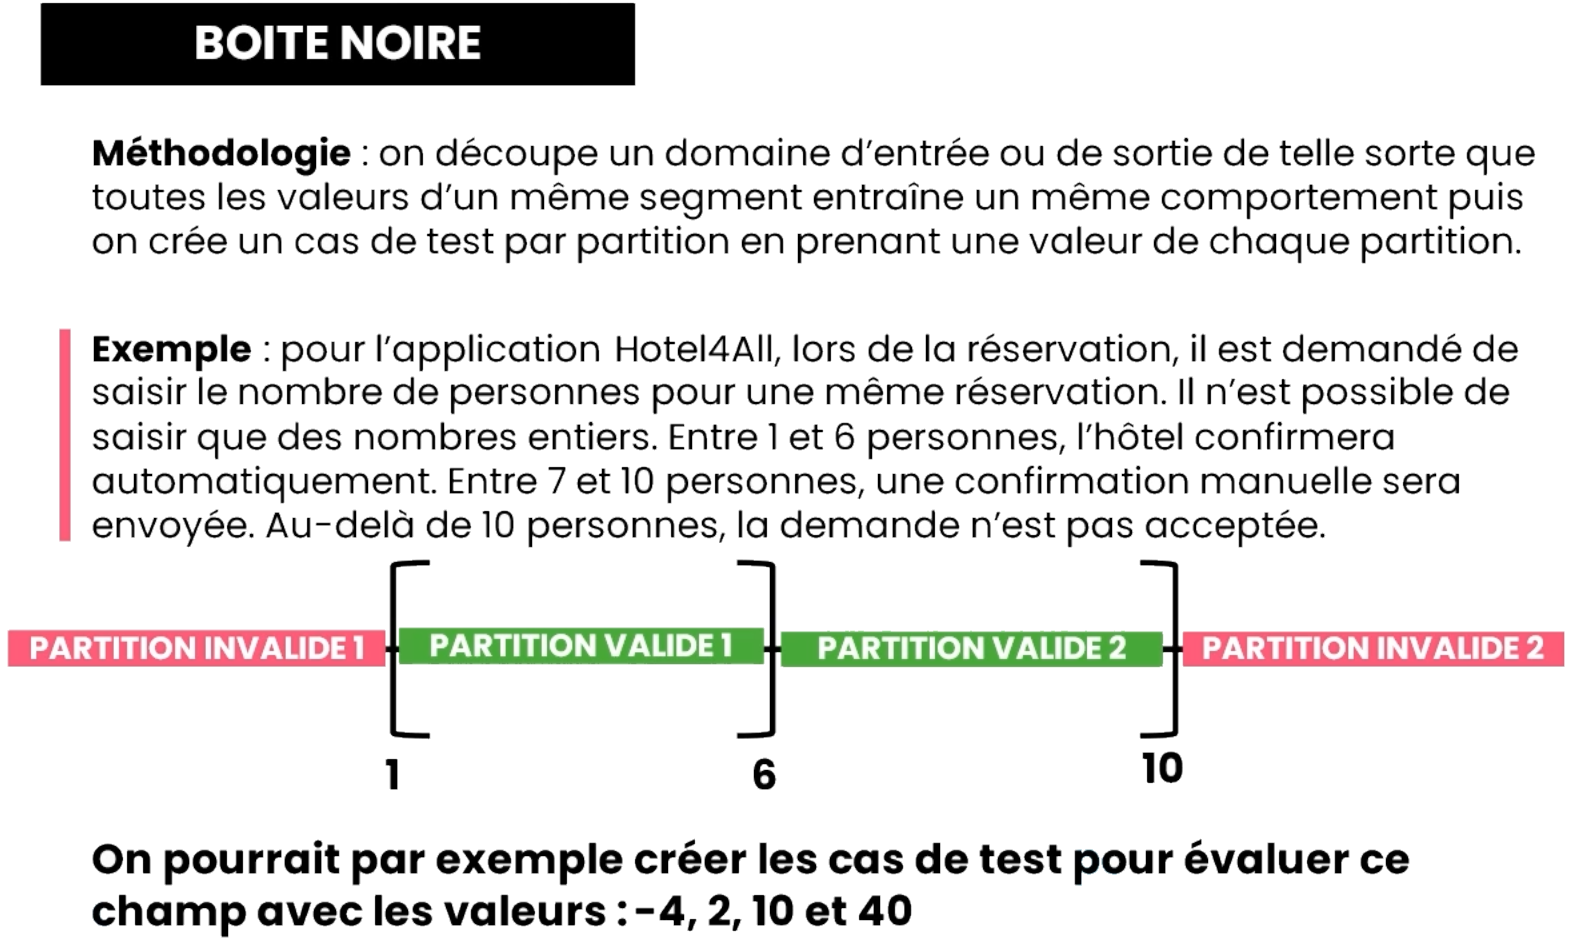
\includegraphics[width=0.9\textwidth]{images/equiv.png}
    \end{center}
    
	\subsection{La technique des valeurs limites}

    \begin{center}
        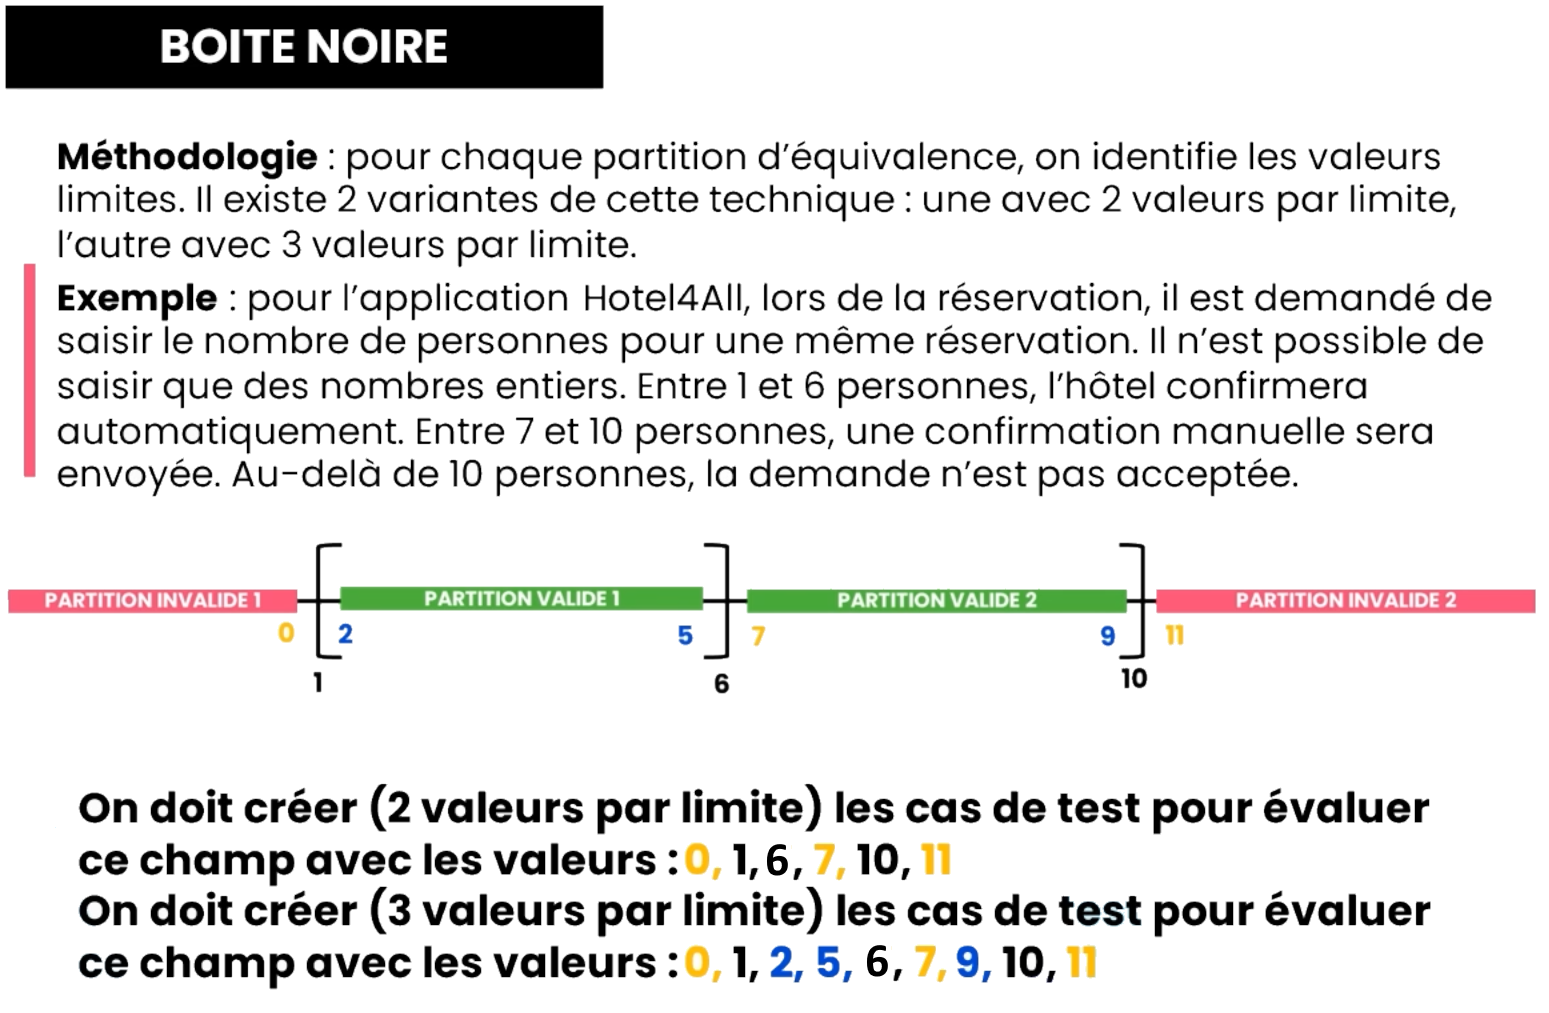
\includegraphics[width=0.9\textwidth]{images/val_lim.png}
    \end{center}
    
	\subsection{La technique des tables de décision}

    \begin{center}
        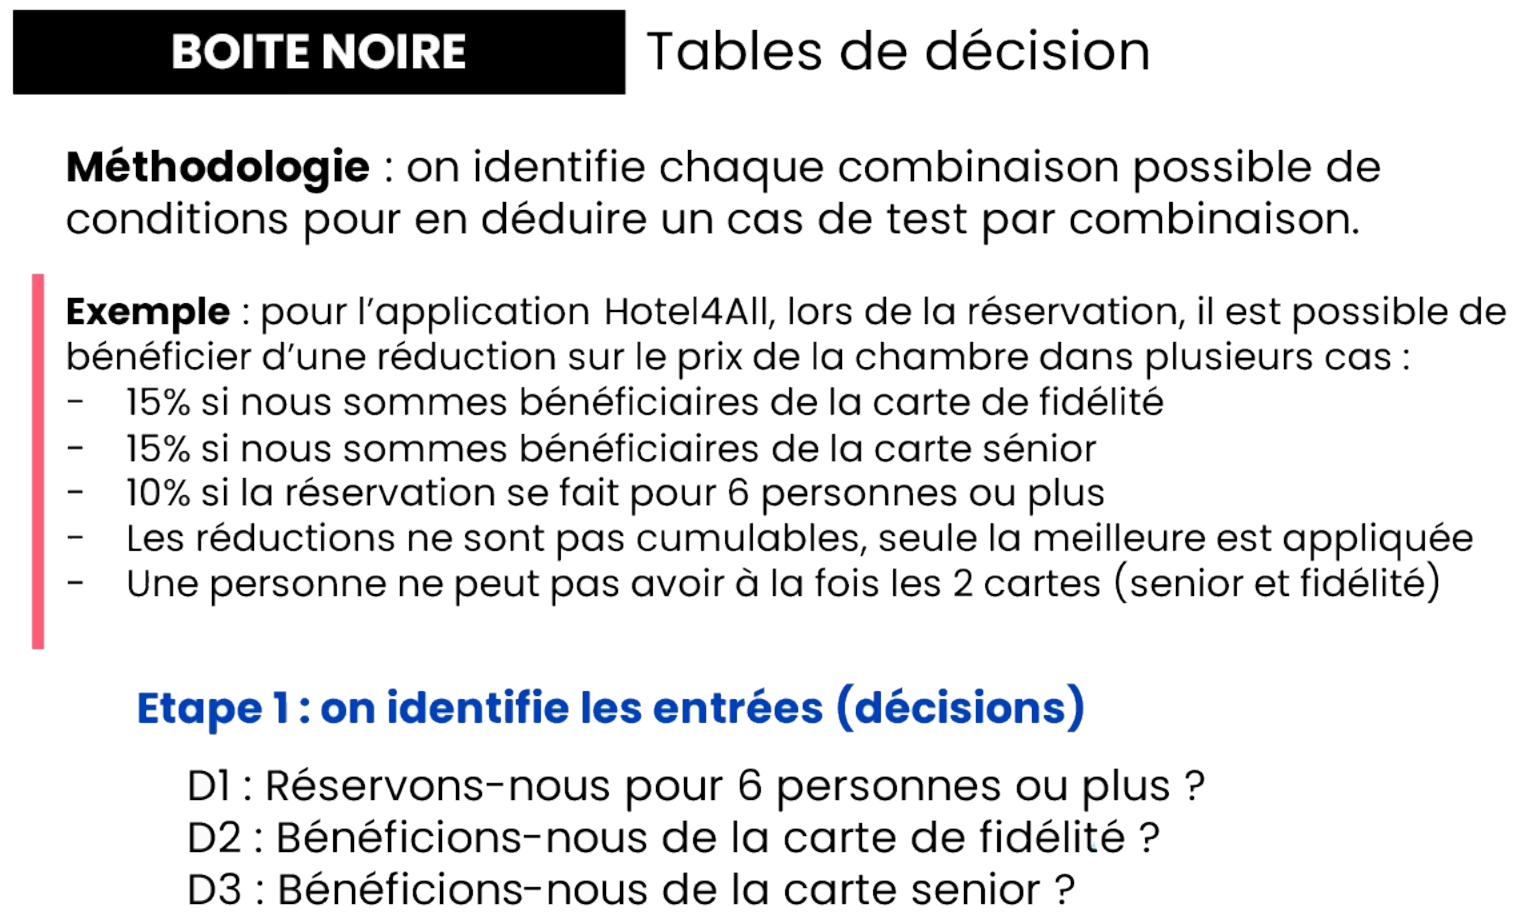
\includegraphics[width=0.9\textwidth]{images/decision_01.png}
        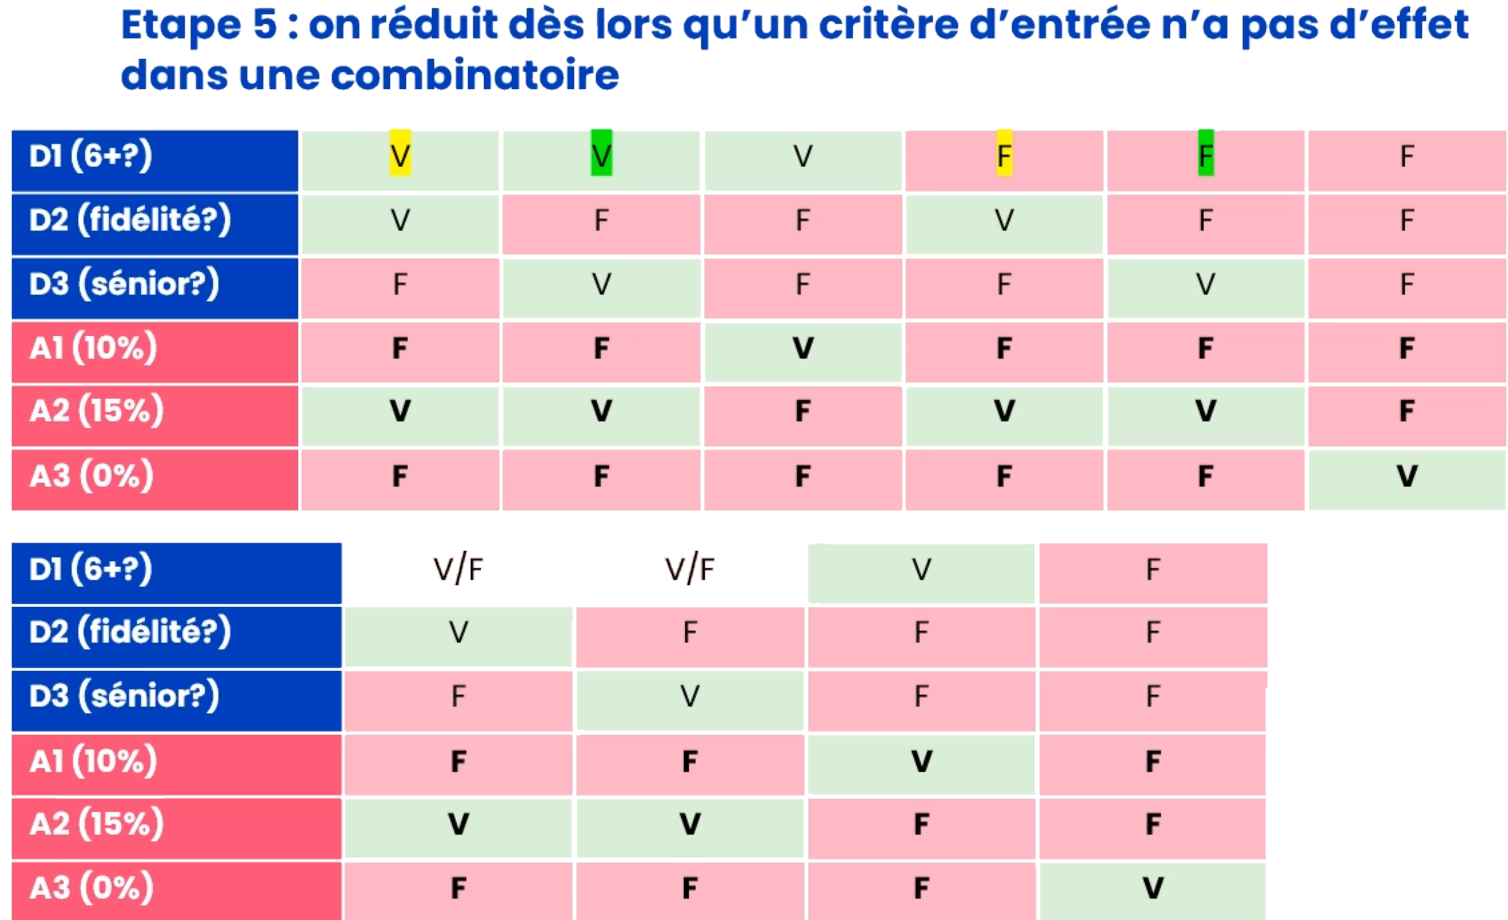
\includegraphics[width=0.9\textwidth]{images/decision_02.png}
\end{center}
    
	\subsection{La technique des transitions d'état}

    \begin{center}
        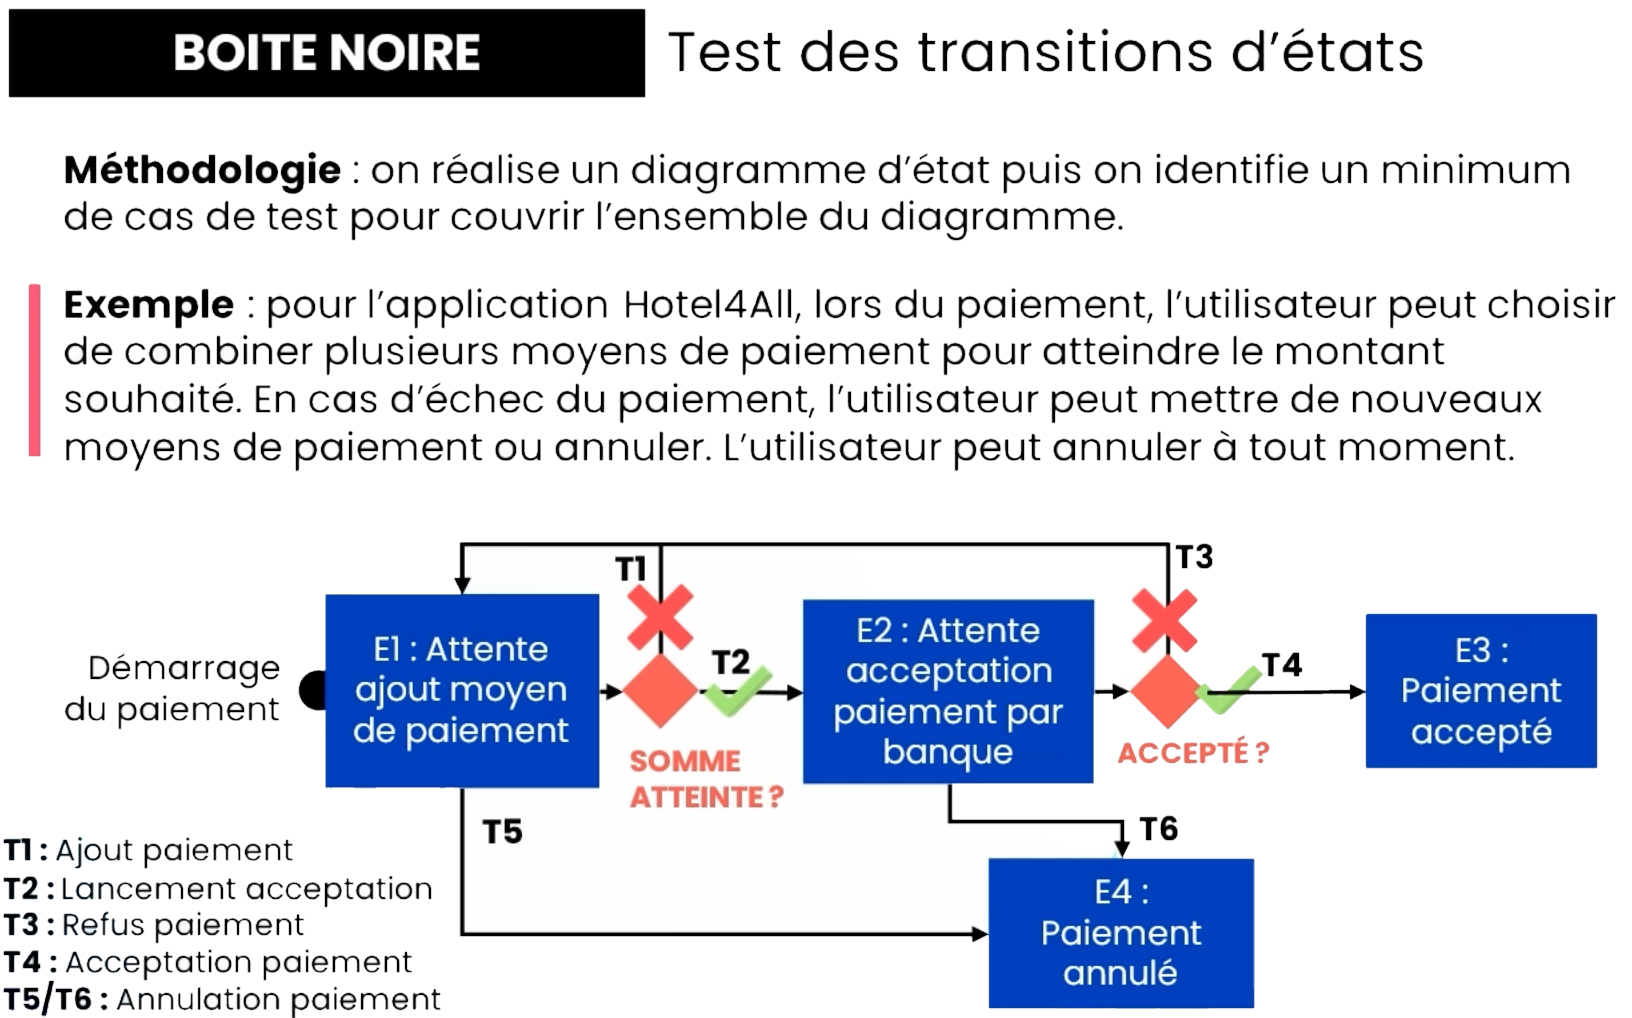
\includegraphics[width=0.9\textwidth]{images/transitions_01.png}
        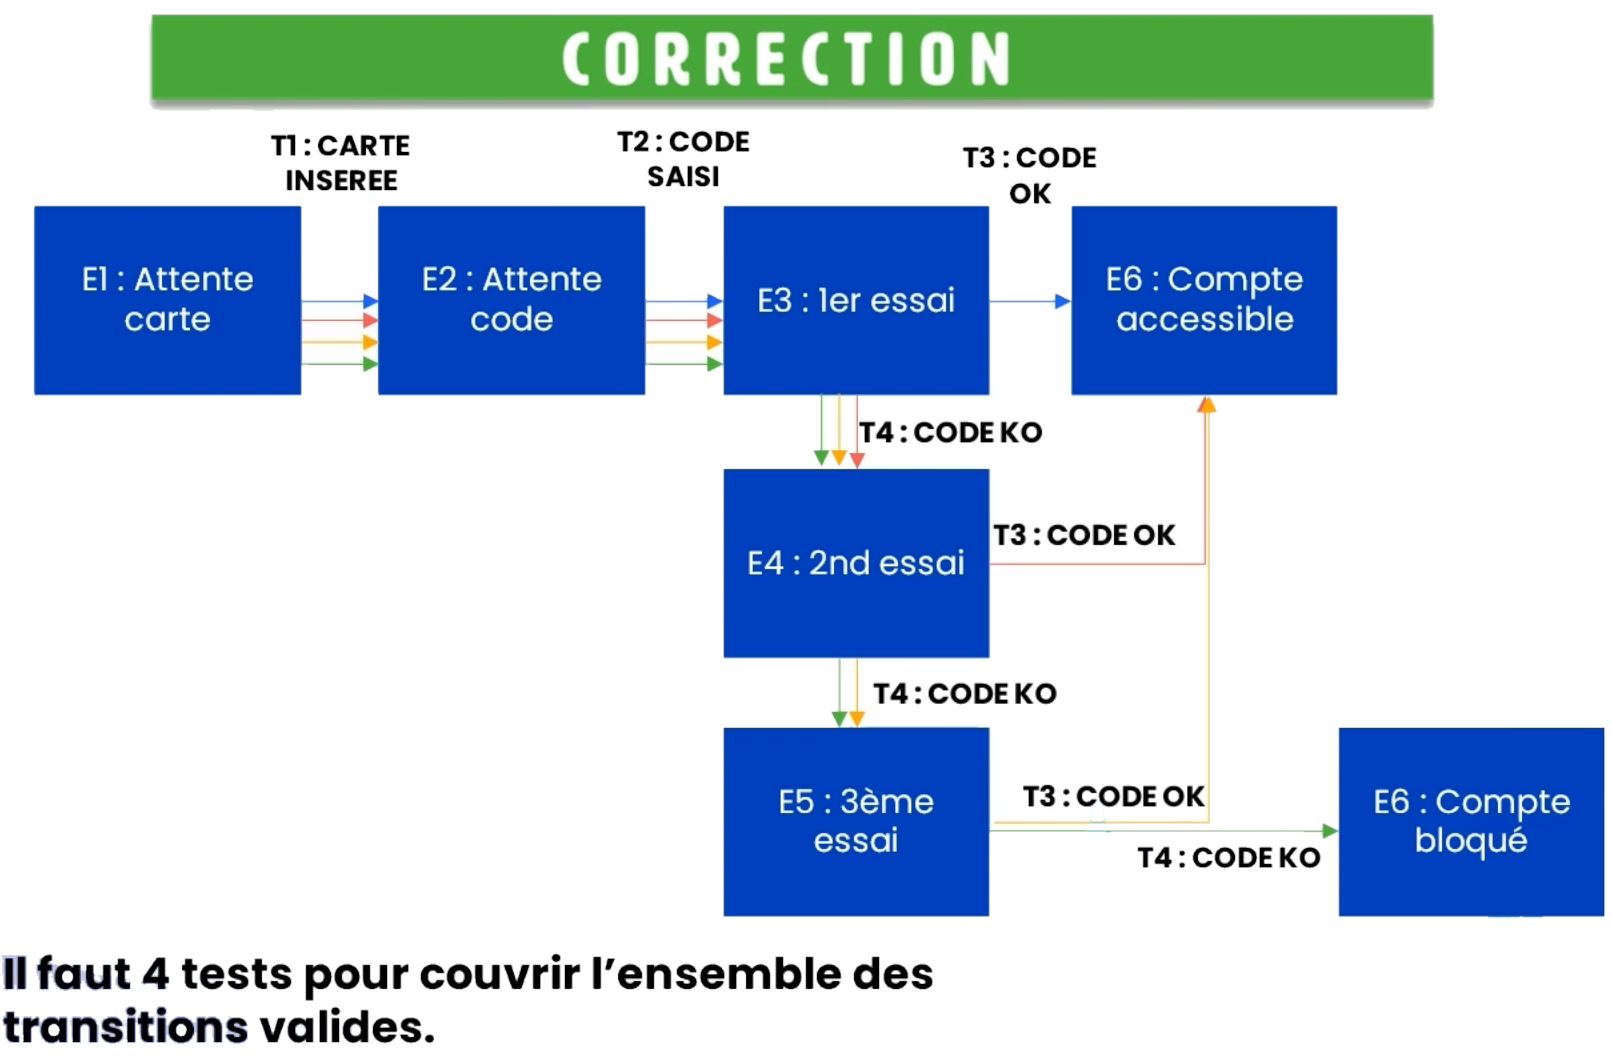
\includegraphics[width=0.9\textwidth]{images/transitions_02.png}
    \end{center}
    
	\subsection{Quelques cas d'utilisation}
    
    \begin{center}
        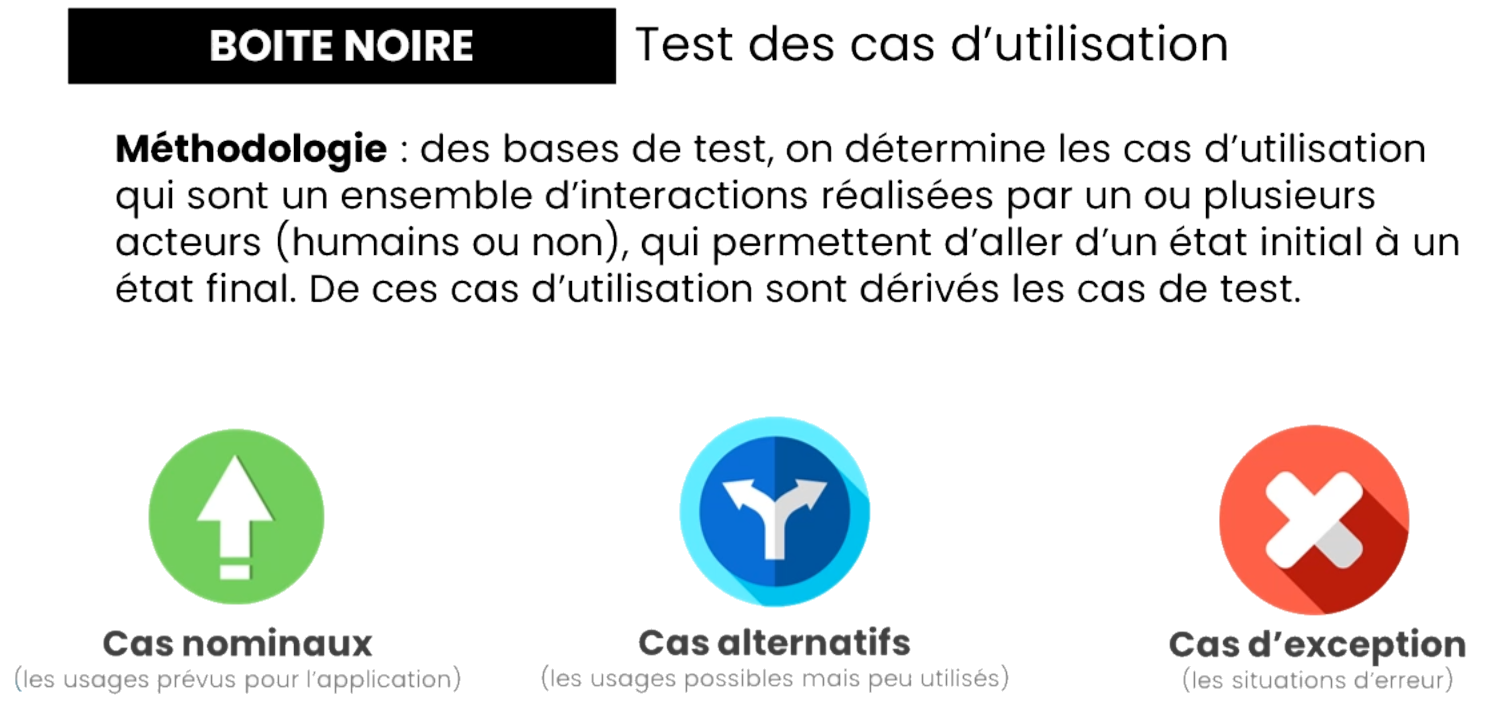
\includegraphics[width=0.9\textwidth]{images/cas_util.png}
    \end{center}
    
	\subsection{Les techniques boîte blanche}

    \begin{center}
        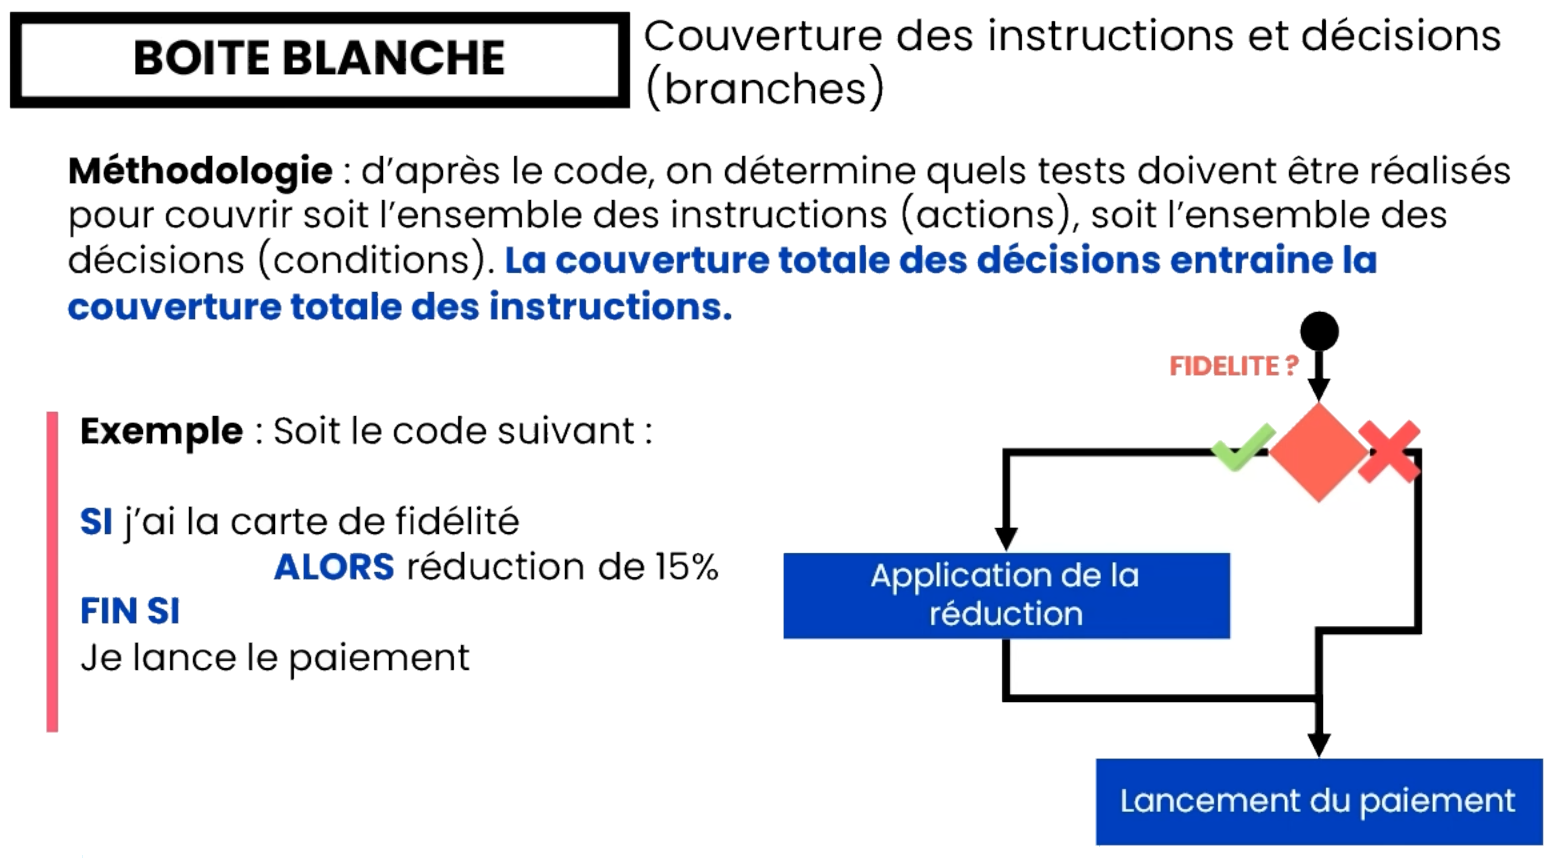
\includegraphics[width=0.9\textwidth]{images/BB_01.png}
        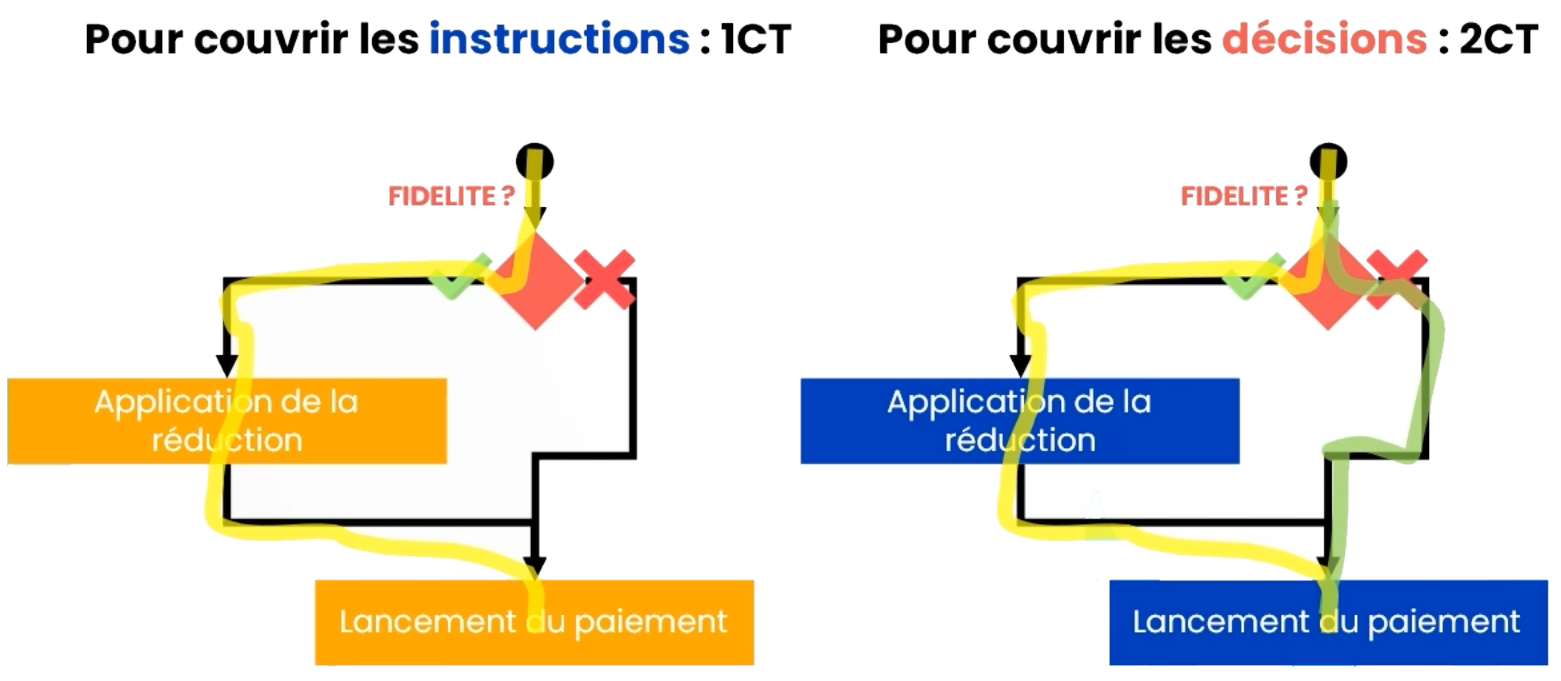
\includegraphics[width=0.9\textwidth]{images/BB_02.png}
        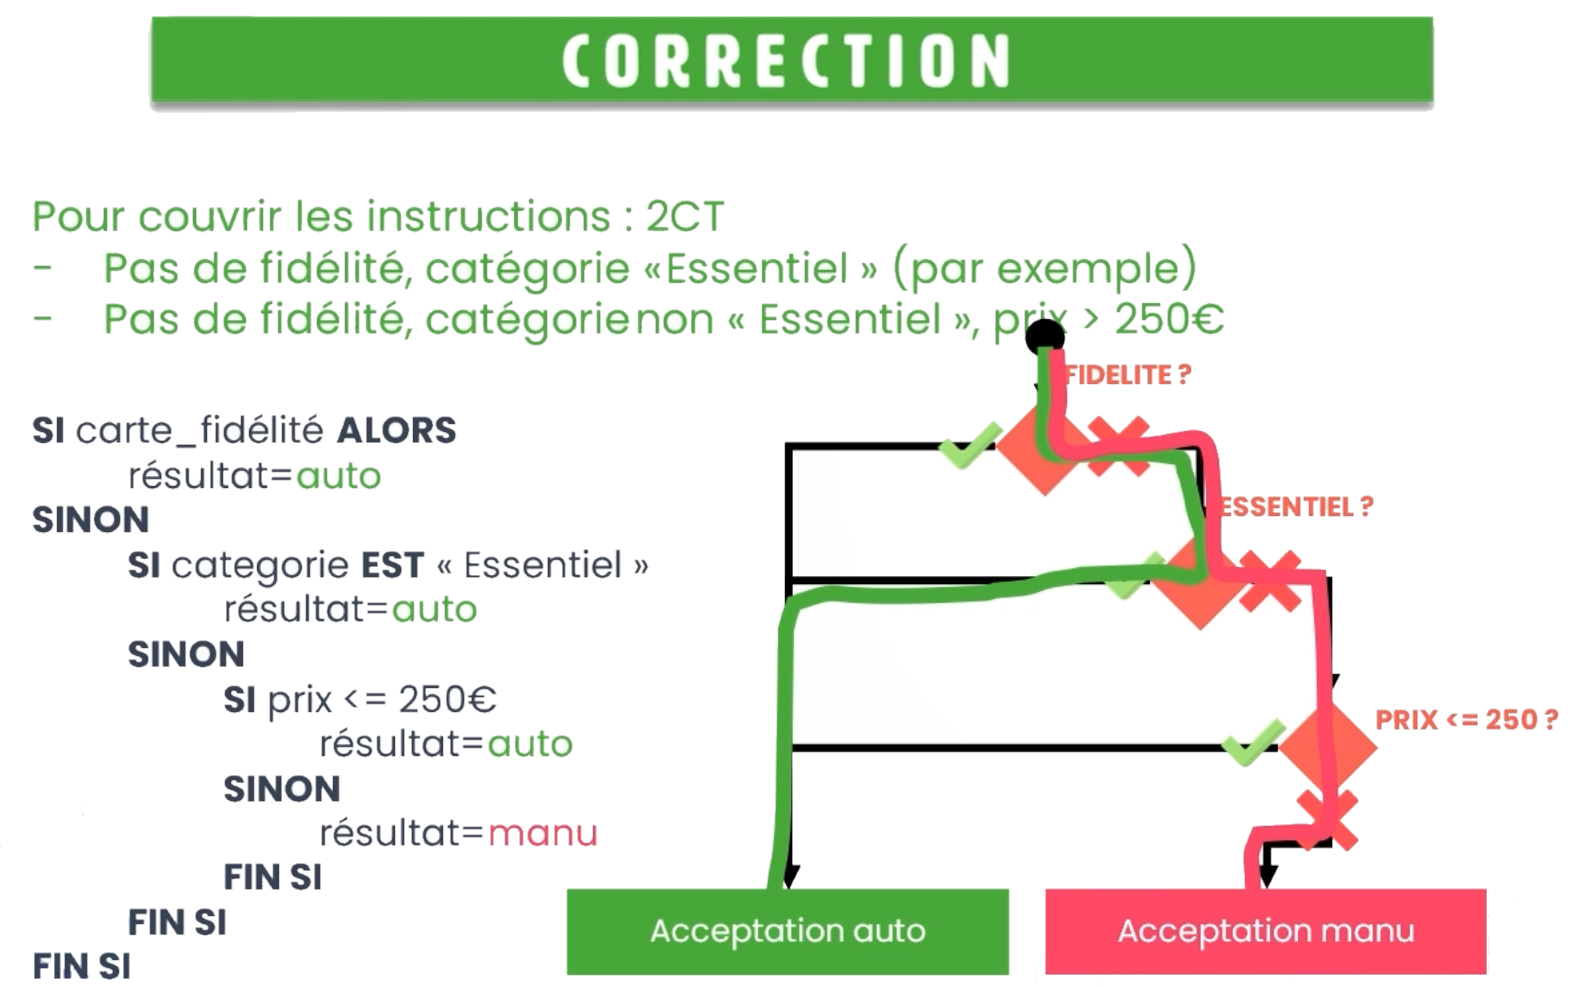
\includegraphics[width=0.9\textwidth]{images/BB_03.png}
    \end{center}
    
	\subsection{Les techniques basées sur l'expérience}

    \begin{center}
        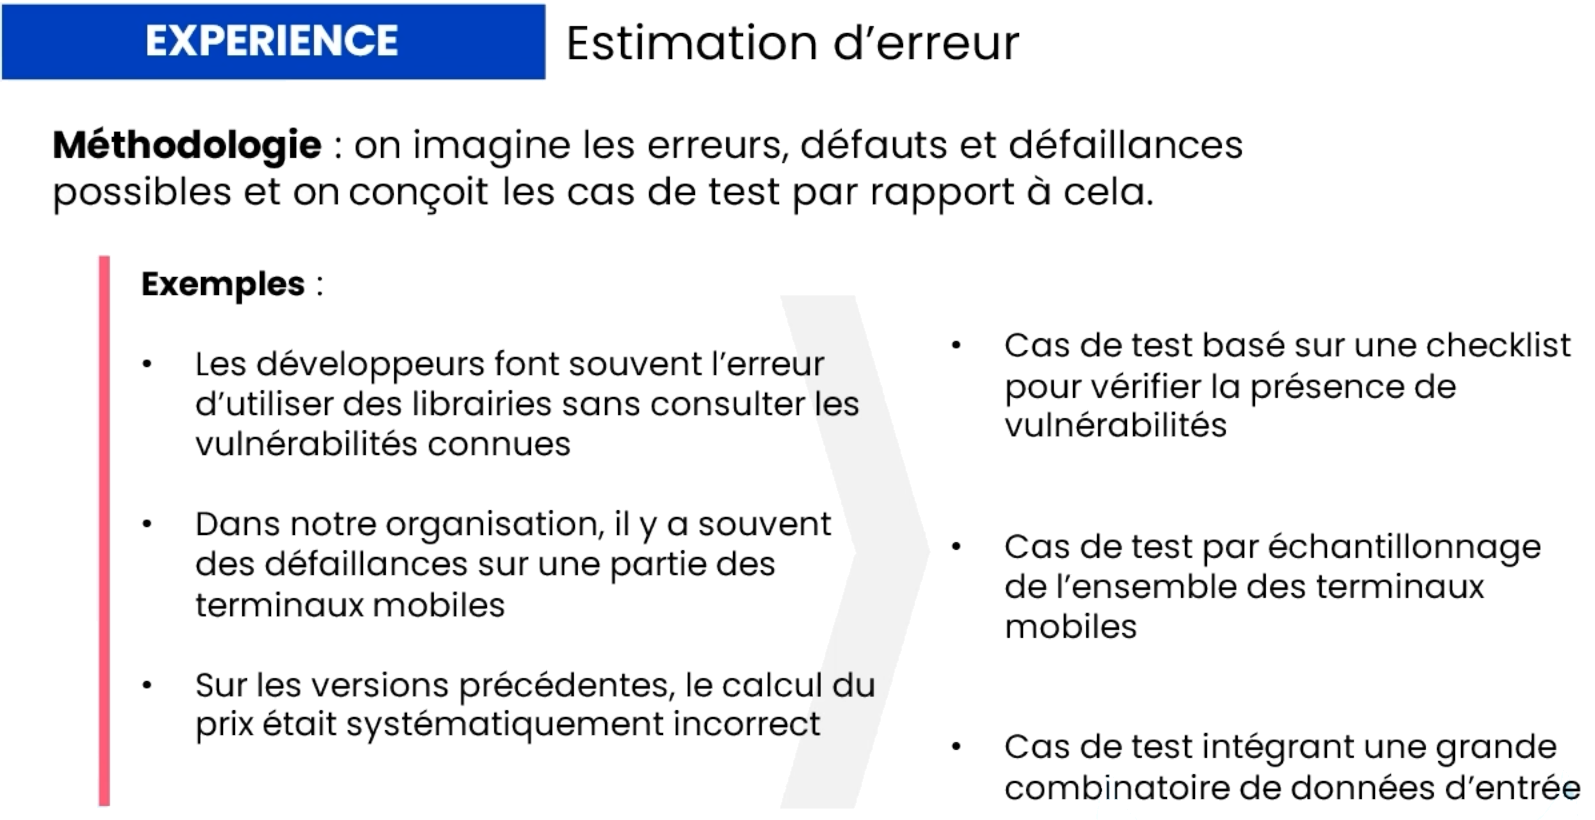
\includegraphics[width=0.9\textwidth]{images/experience_01.png}
        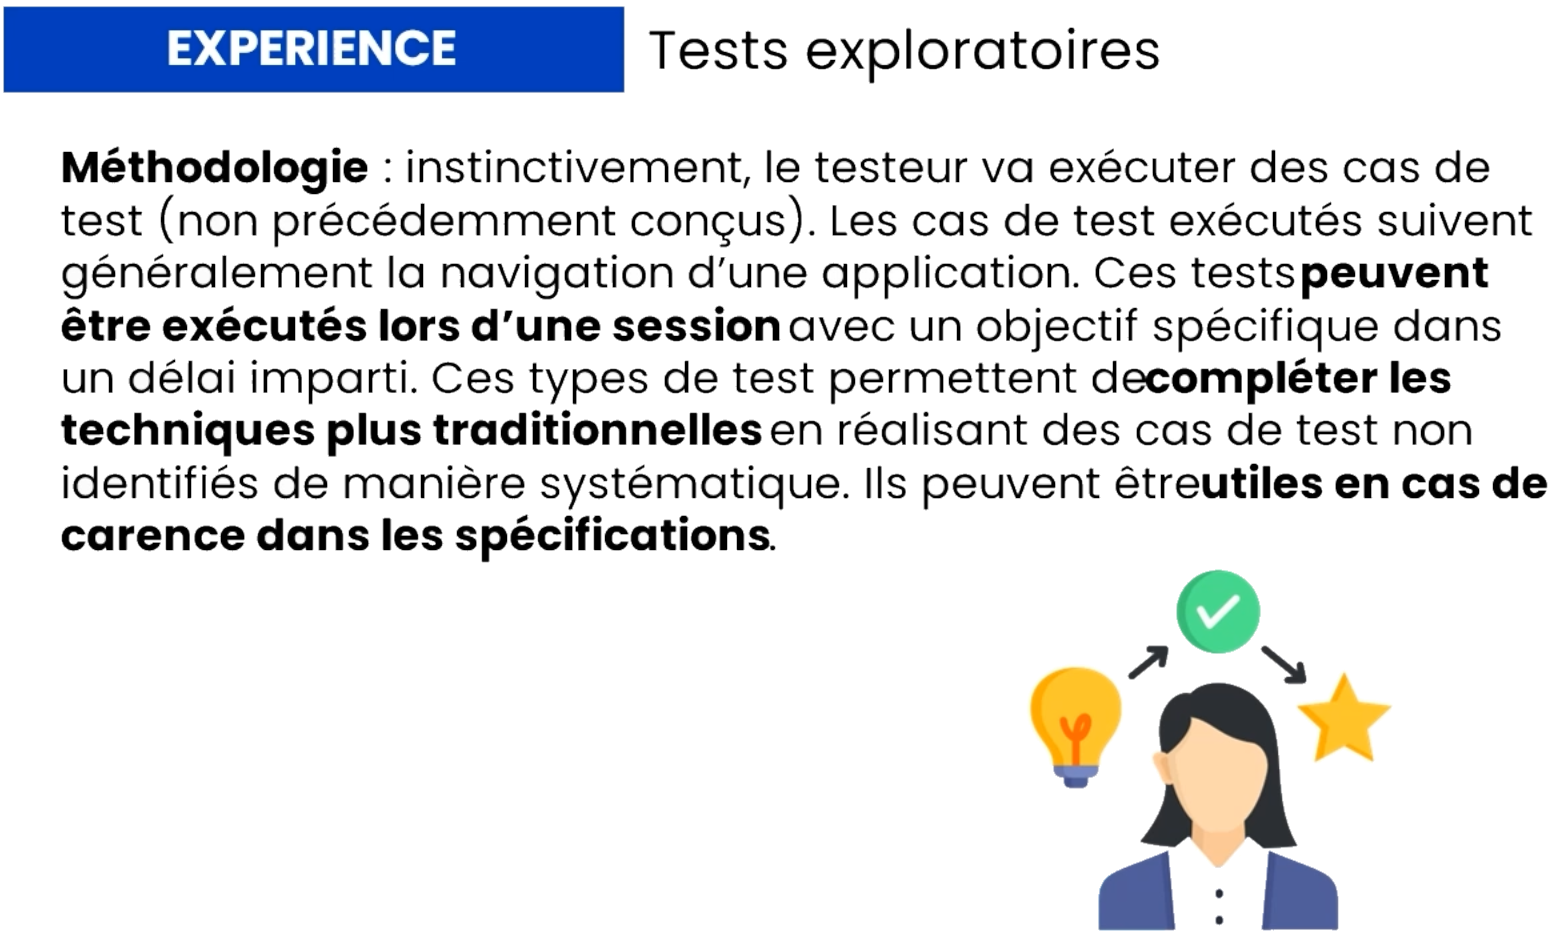
\includegraphics[width=0.9\textwidth]{images/experience_02.png}
        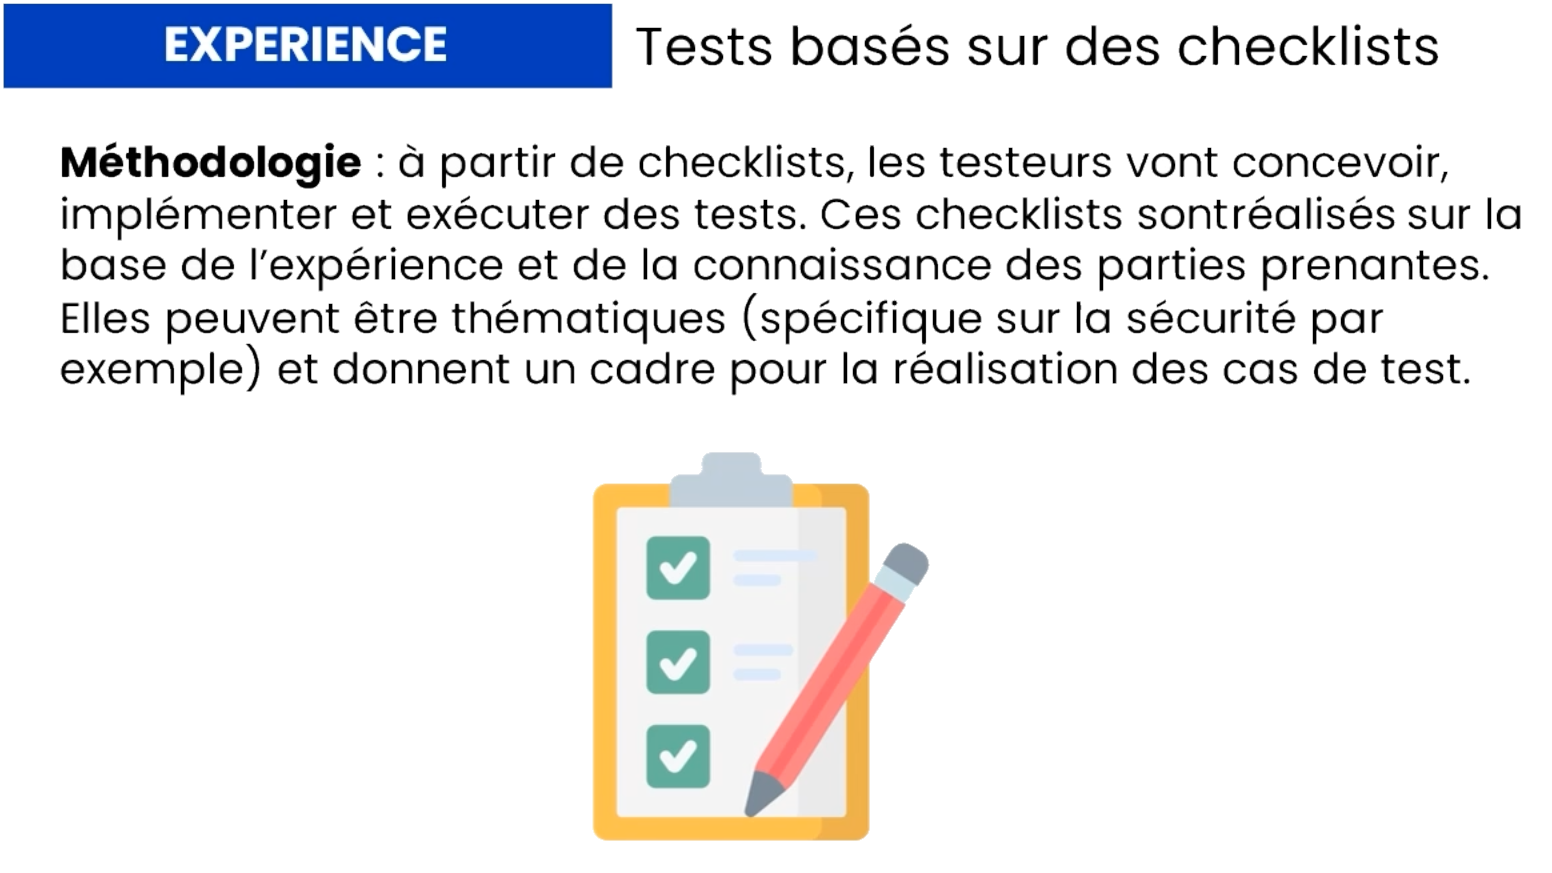
\includegraphics[width=0.9\textwidth]{images/experience_03.png}
    \end{center}
    
	\subsection{Les User Stories (US) et les critères d'acceptation}

    \begin{center}
        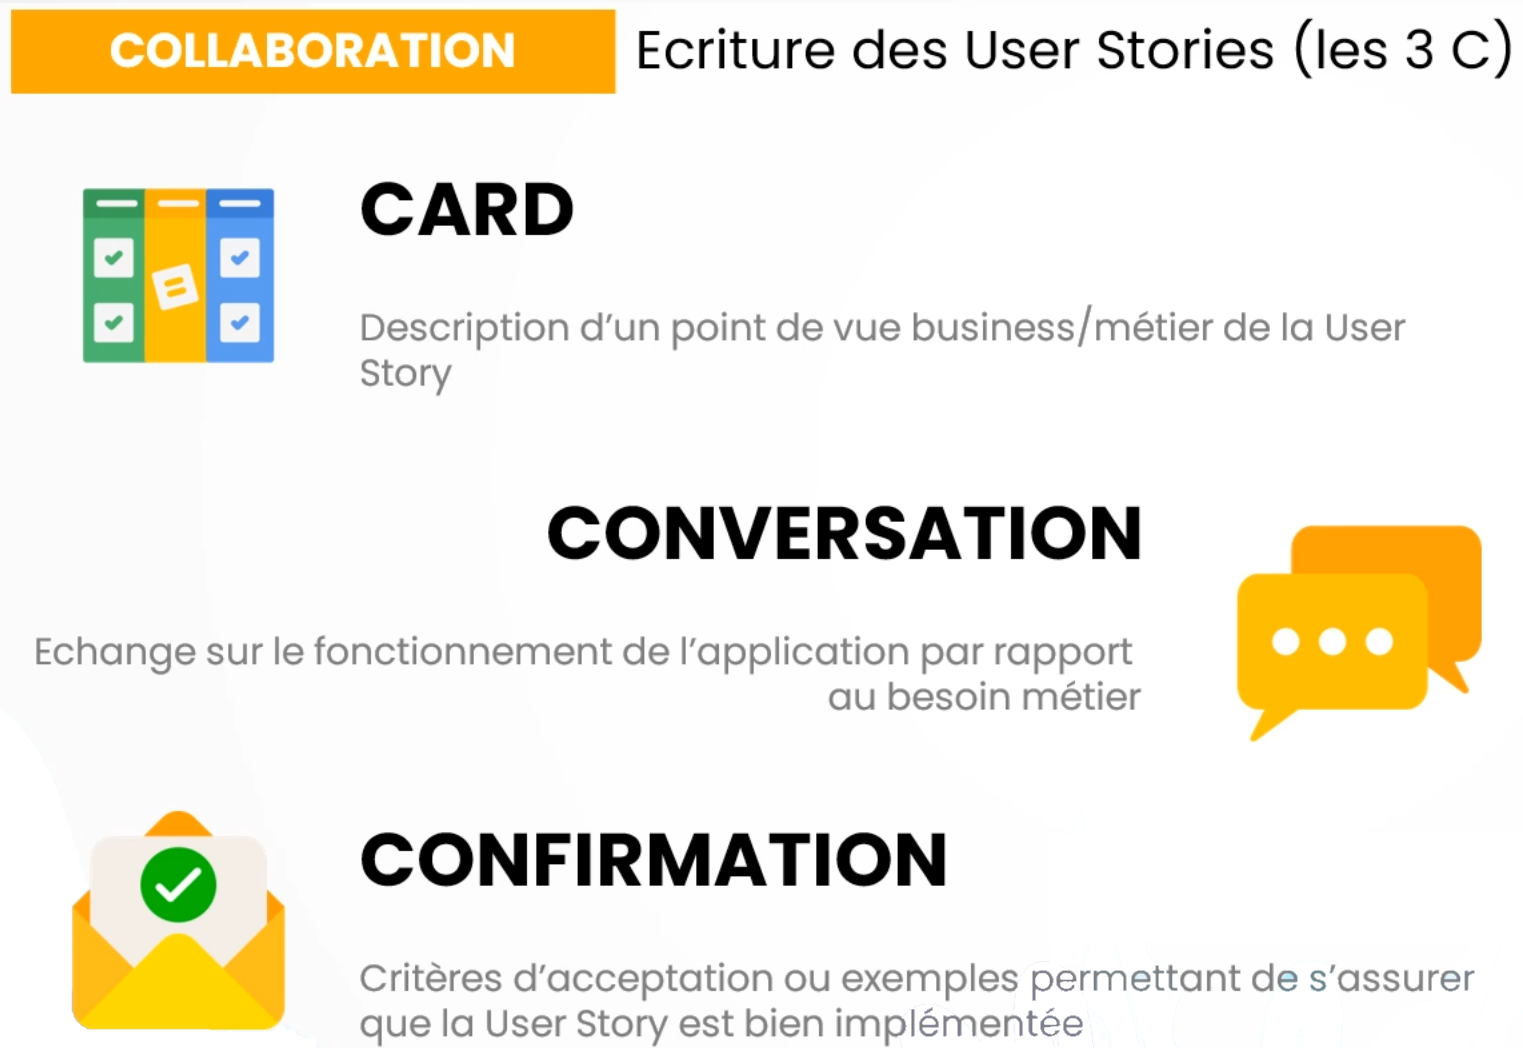
\includegraphics[width=0.9\textwidth]{images/US_01.png}
        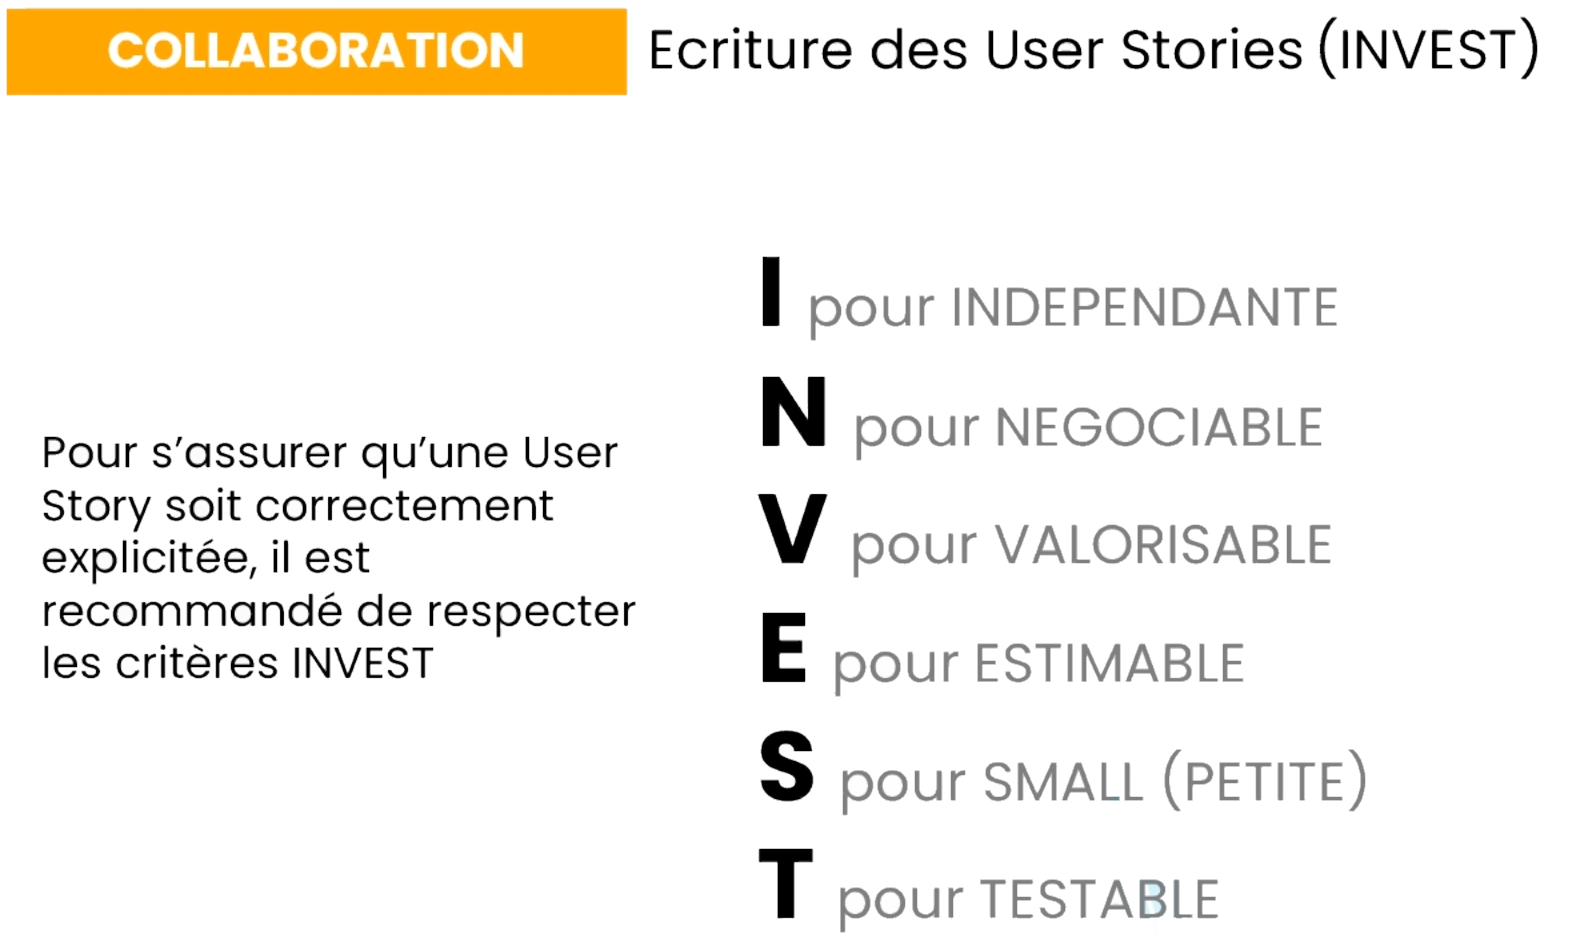
\includegraphics[width=0.9\textwidth]{images/US_02.png}
        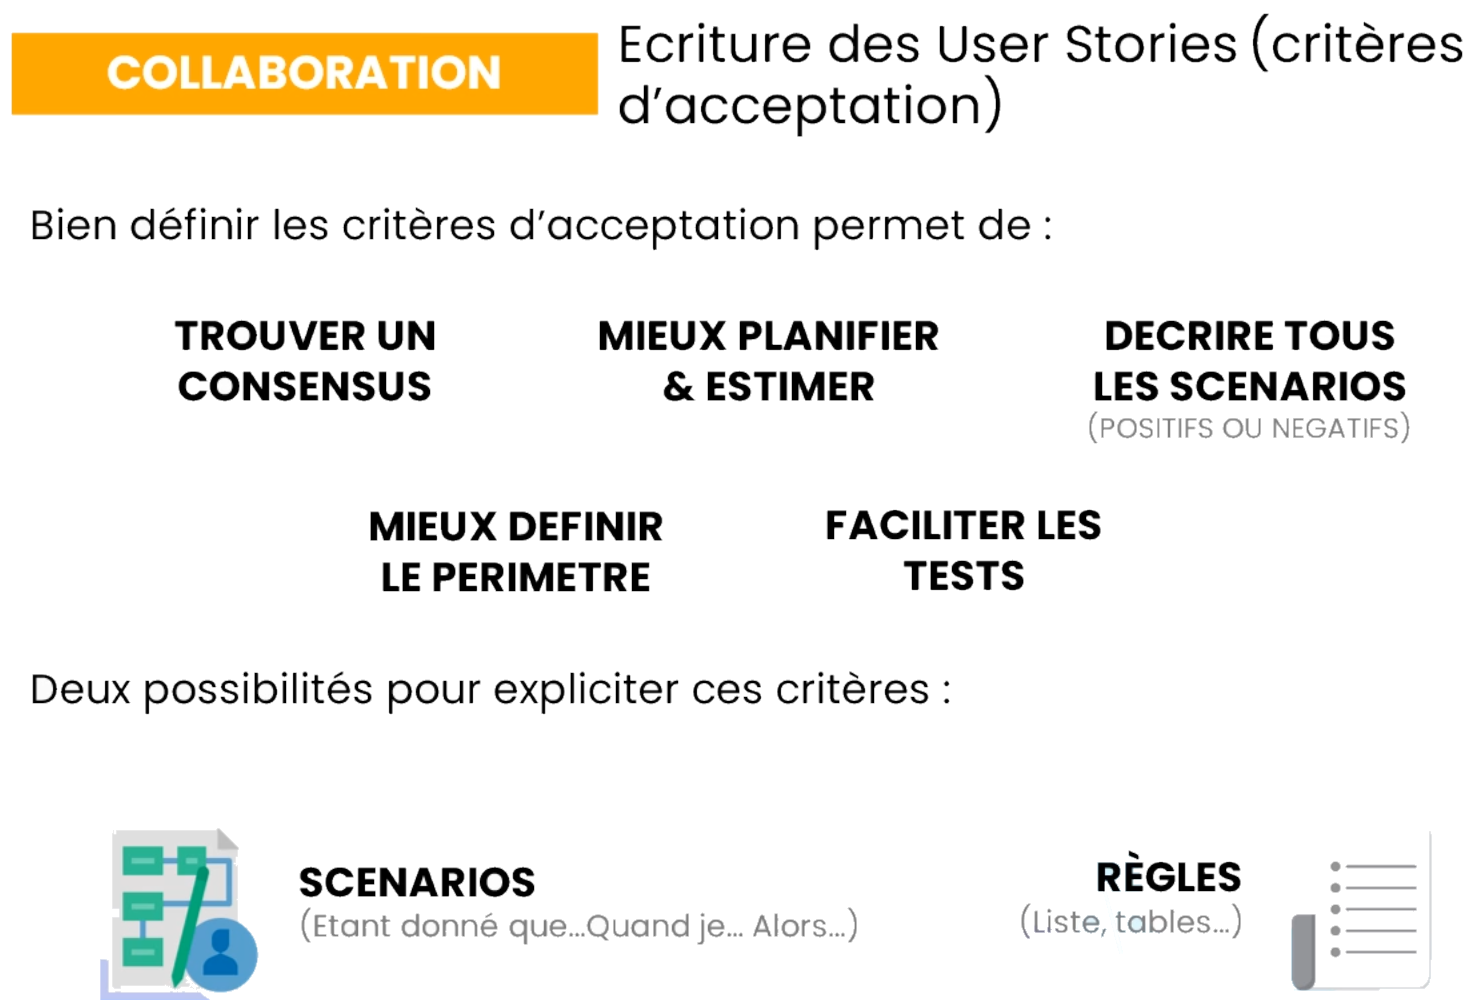
\includegraphics[width=0.9\textwidth]{images/US_03.png}
    \end{center}
    
	\subsection{L'ATDD (Acceptance Test Driven Development)}

    \begin{center}
        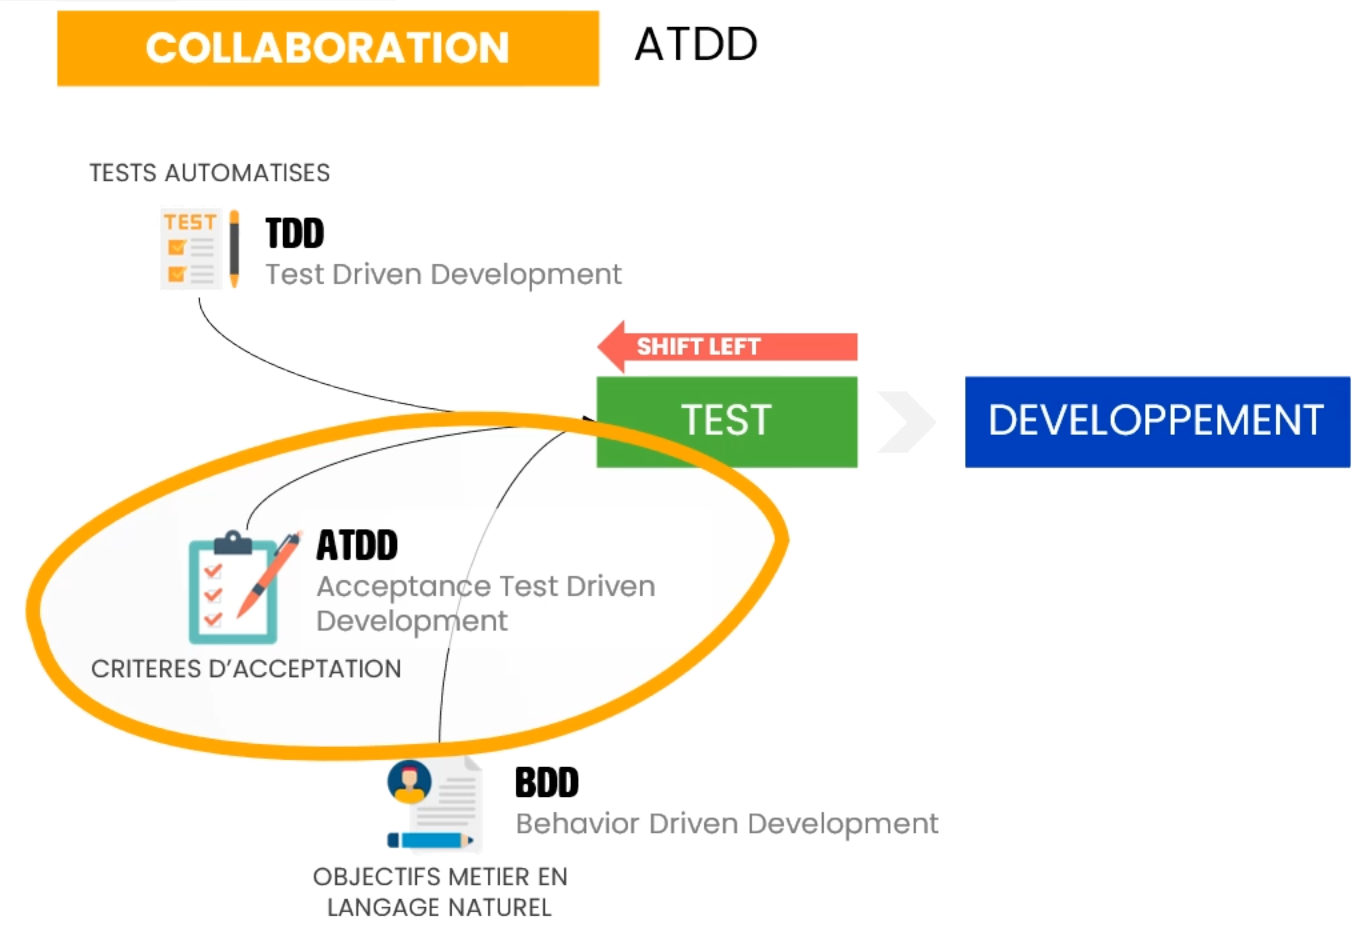
\includegraphics[width=0.9\textwidth]{images/ATDD_01.png}
        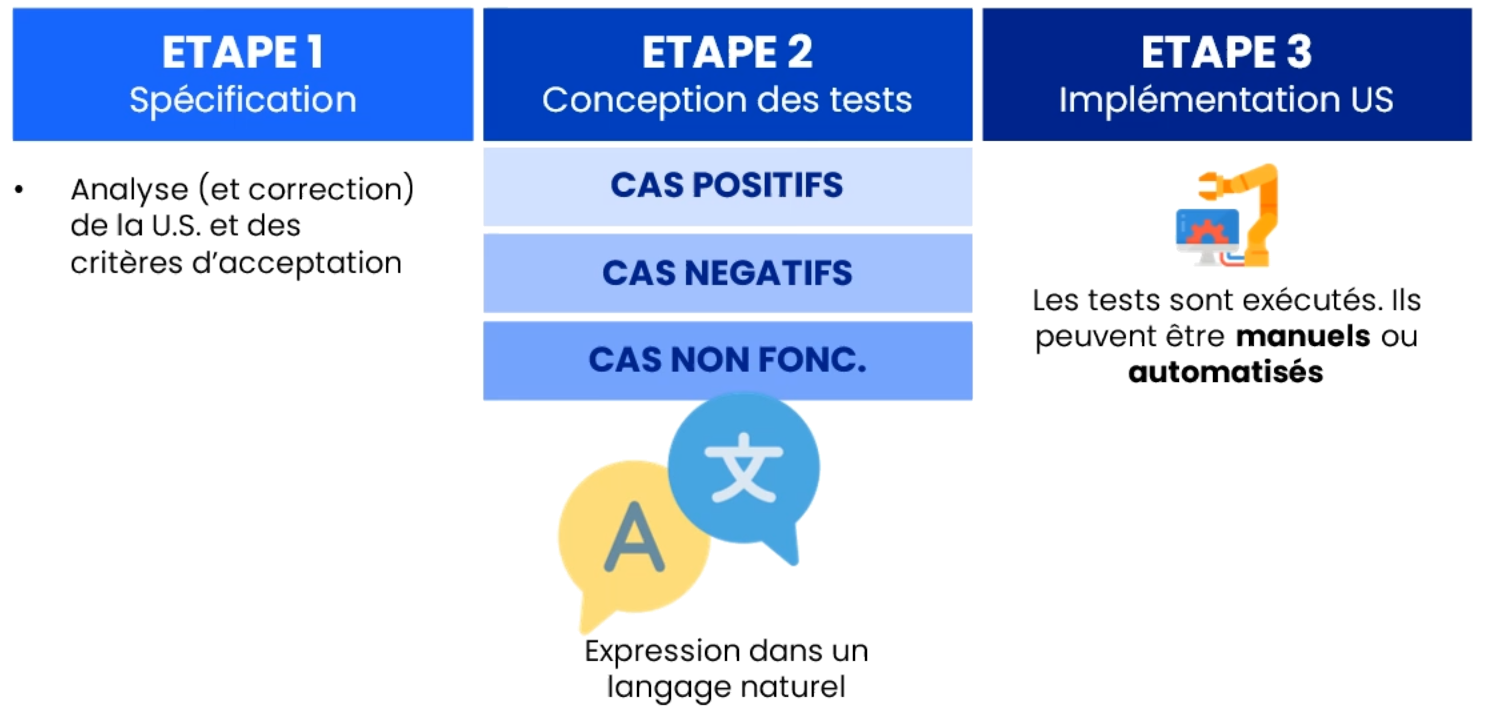
\includegraphics[width=0.9\textwidth]{images/ATDD_02.png}
    \end{center}



\pagebreak
\section{GESTION DES TESTS}

	\subsection{Le plan de test}

    \begin{center}
        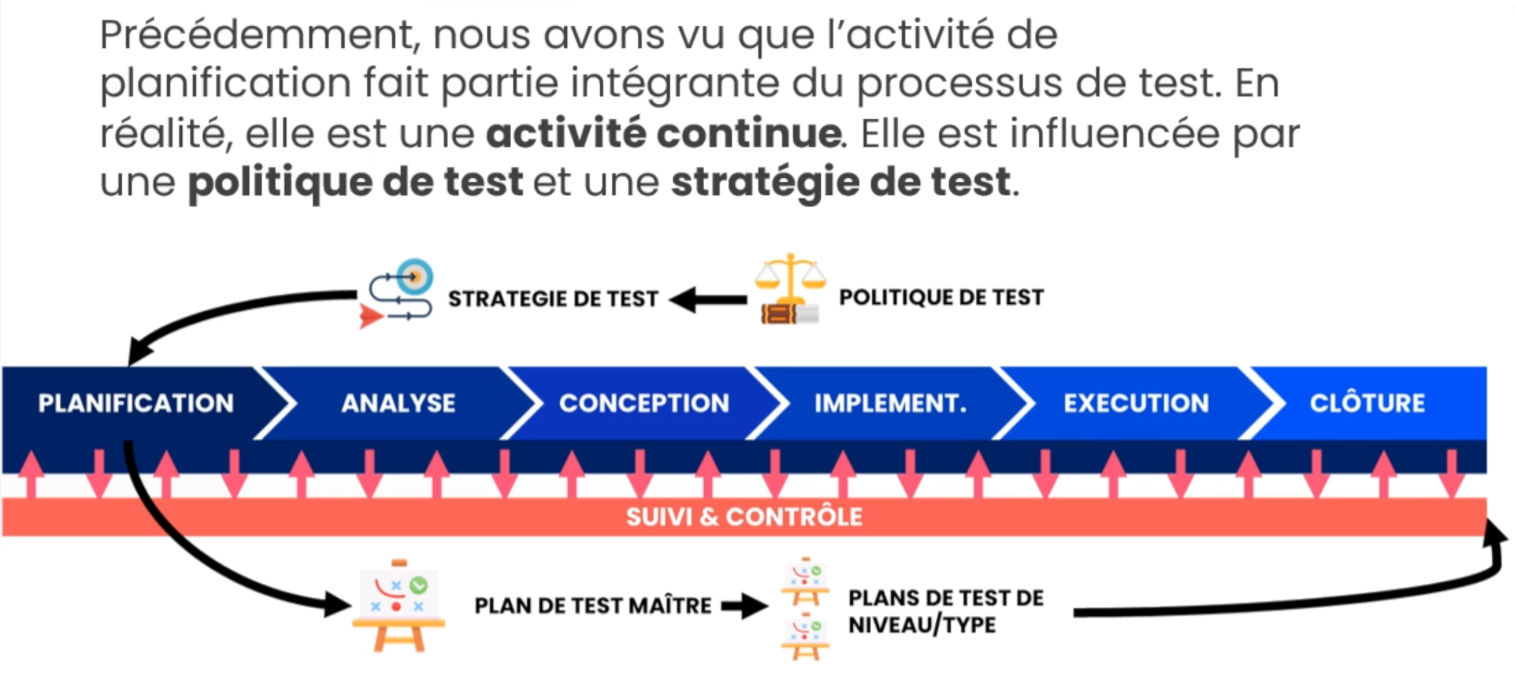
\includegraphics[width=0.9\textwidth]{images/Plan_de_test_01.png}
        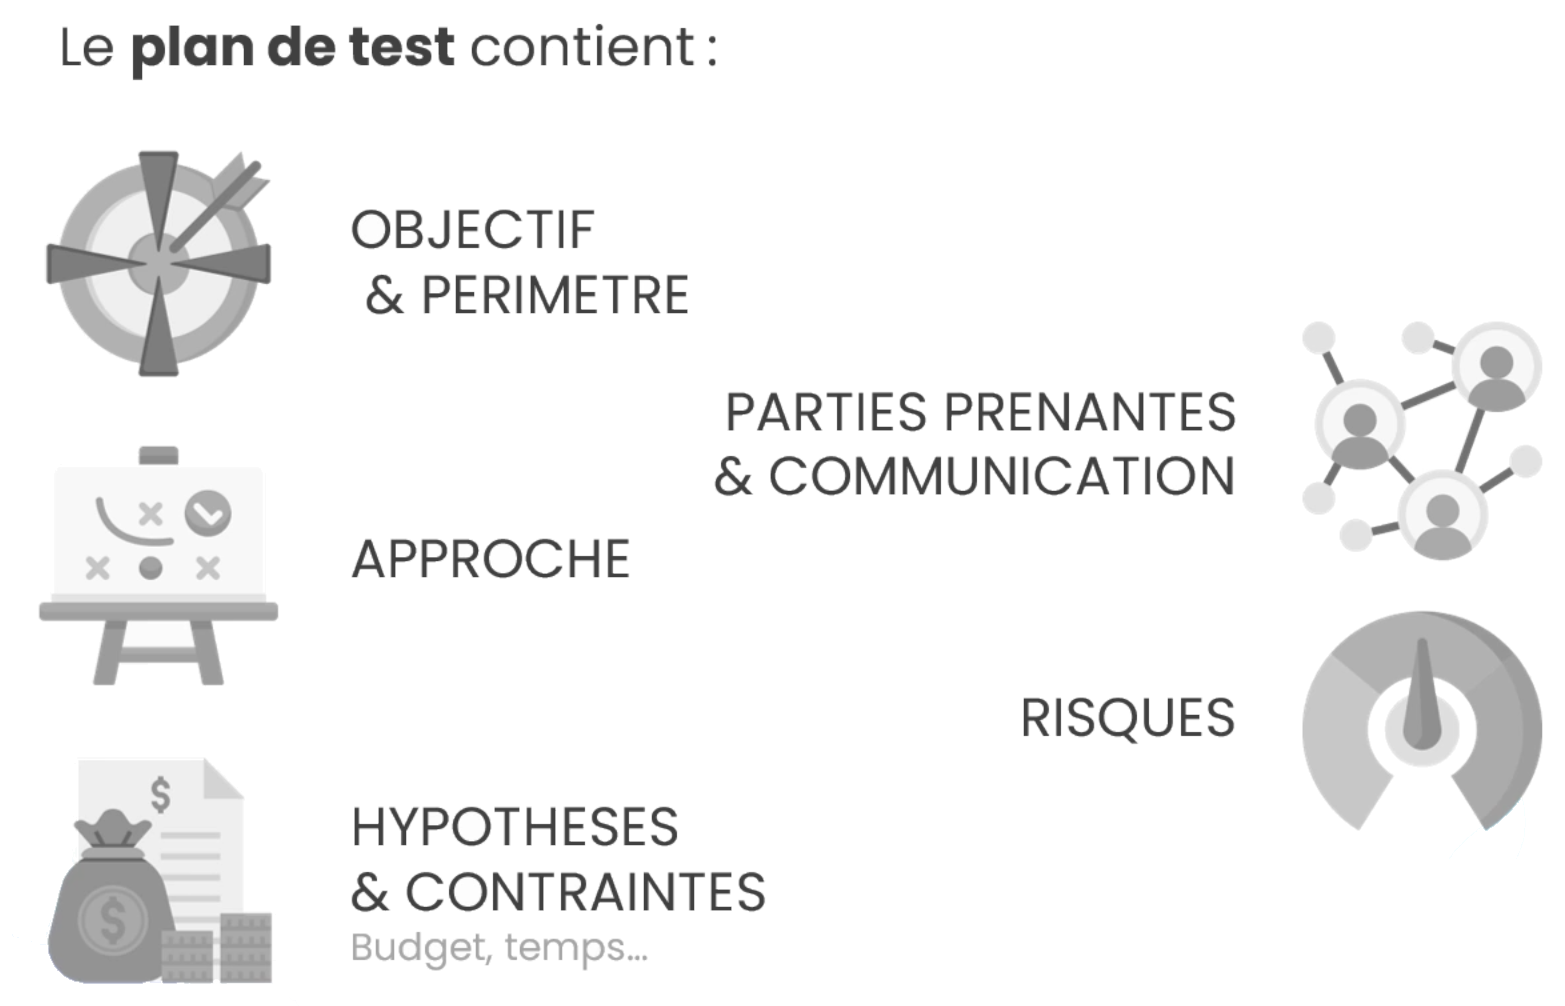
\includegraphics[width=0.9\textwidth]{images/Plan_de_test_02.png}
        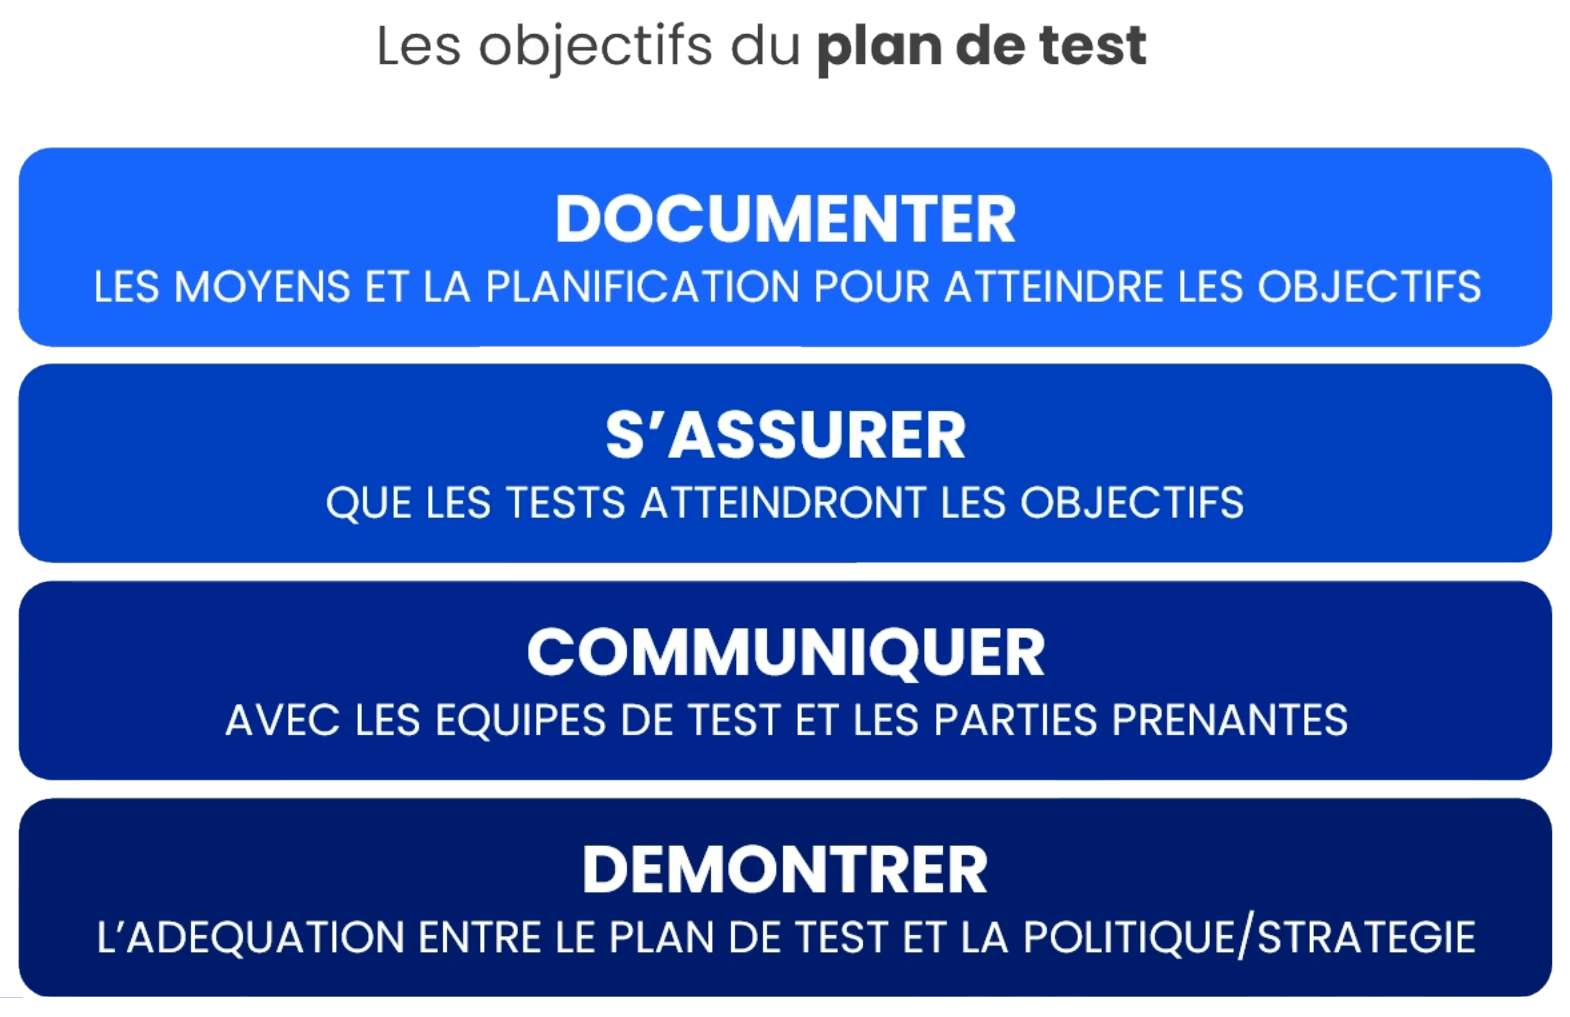
\includegraphics[width=0.9\textwidth]{images/Plan_de_test_03.png}
        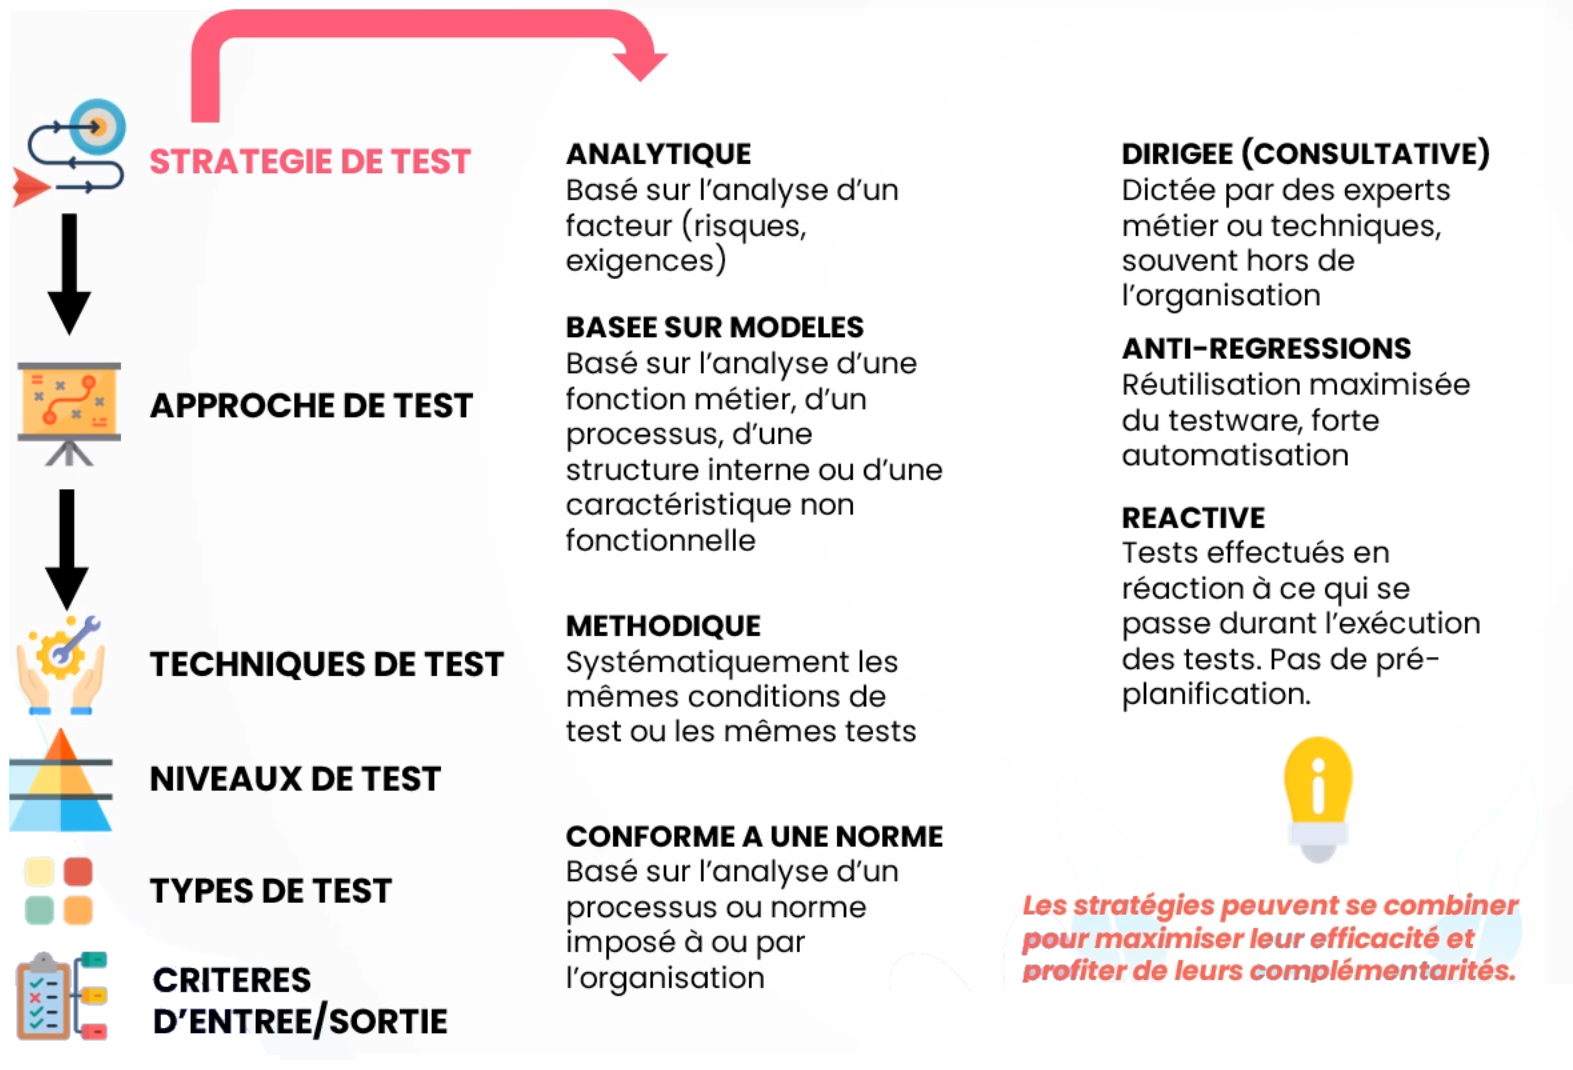
\includegraphics[width=0.9\textwidth]{images/Plan_de_test_04.png}
    \end{center}
    
	\subsection{La contribution des testeurs et la planification}

    \begin{center}
        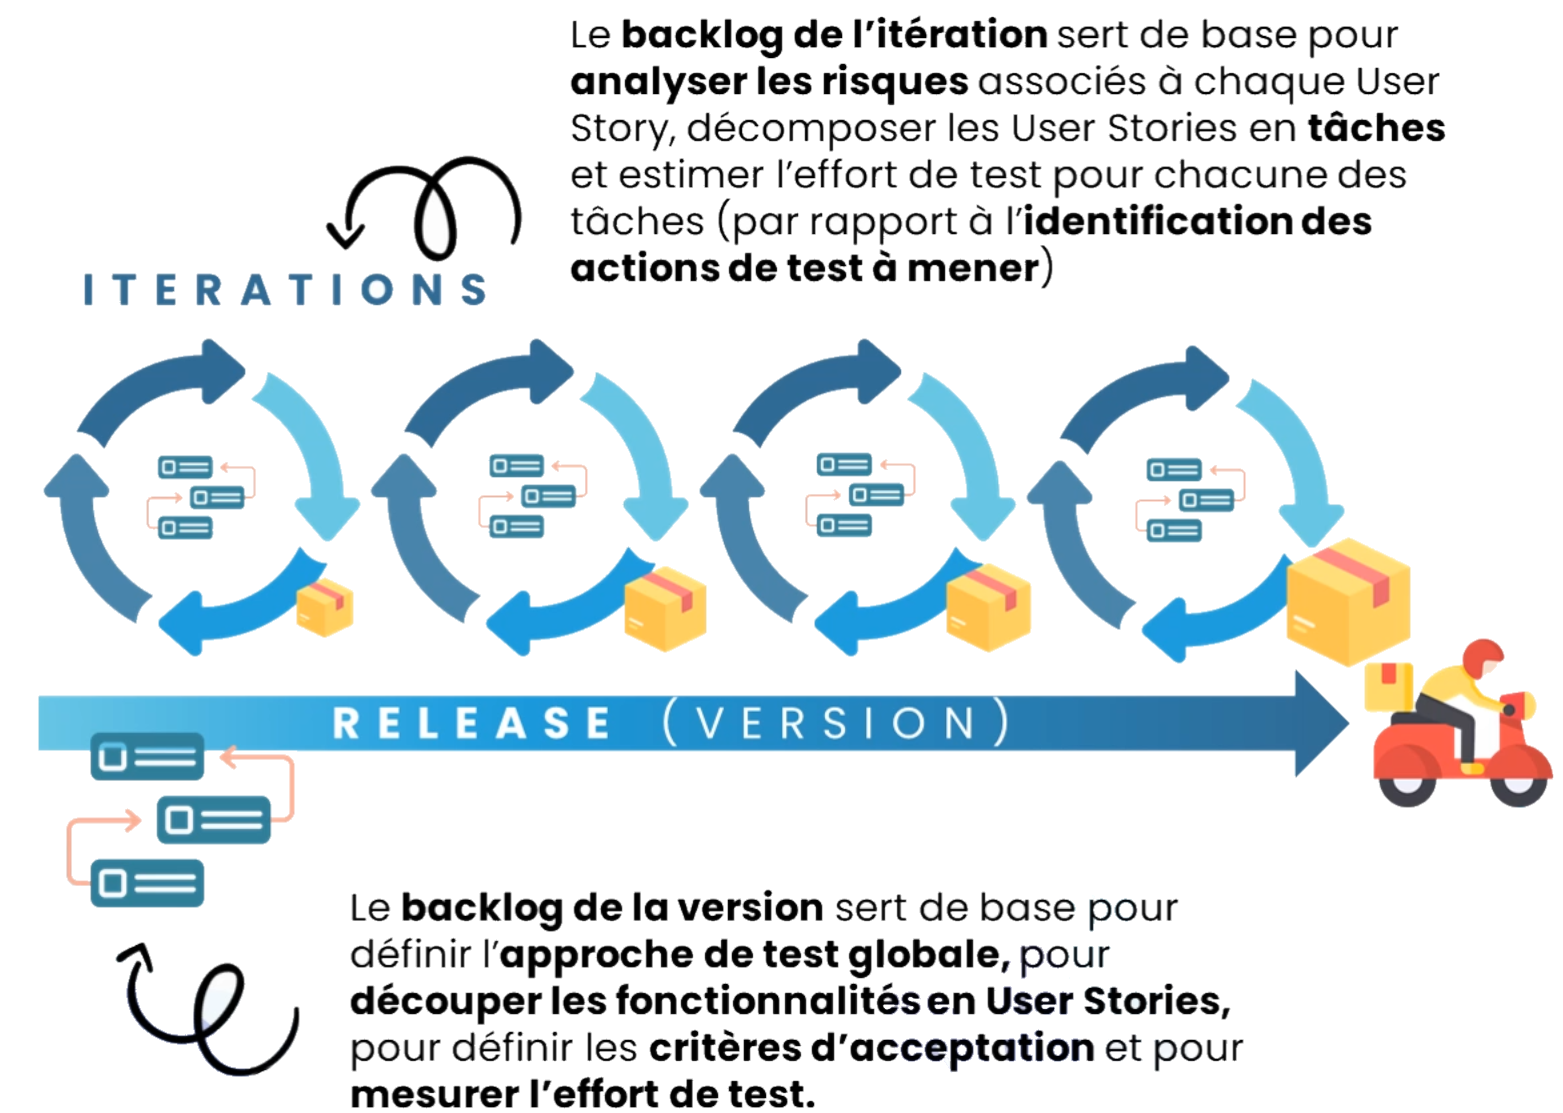
\includegraphics[width=0.9\textwidth]{images/contrib_testeur_plan.png}
    \end{center}
    
	\subsection{Les critères d'entrée/sortie}

    \begin{center}
        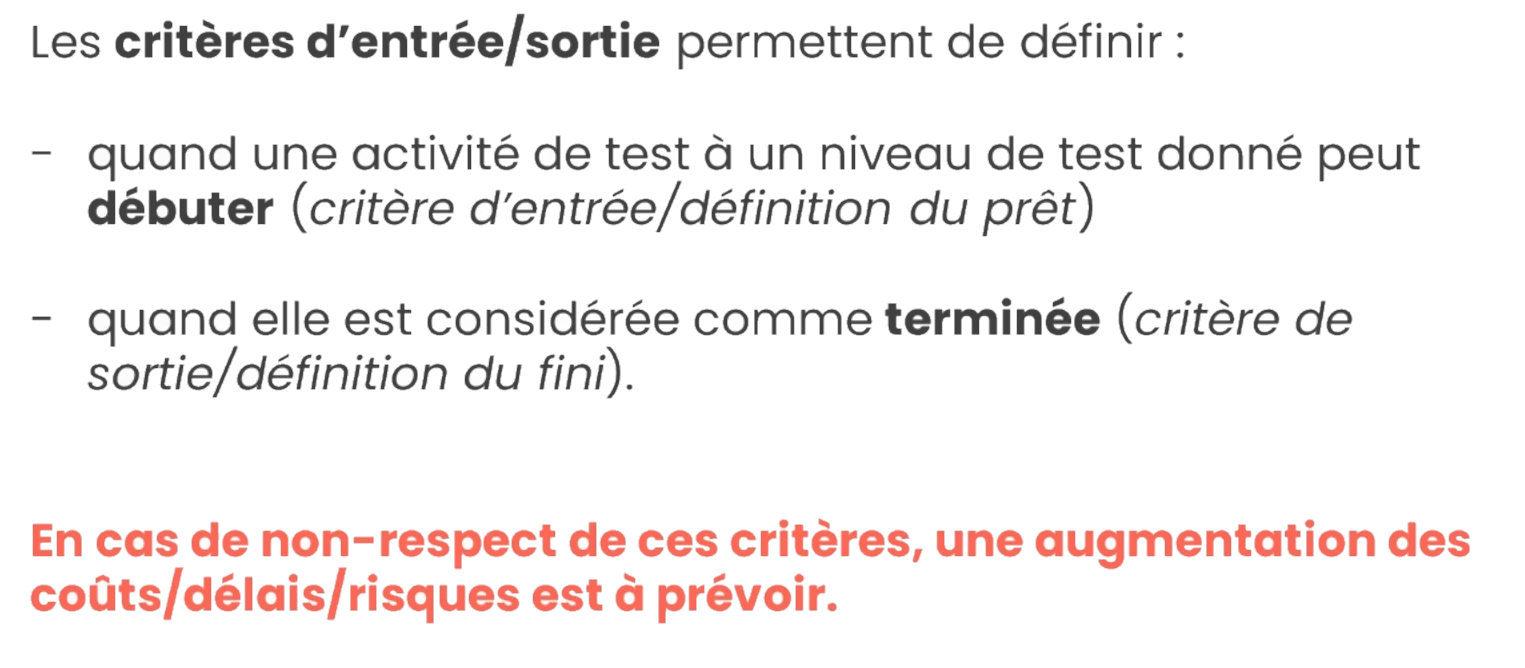
\includegraphics[width=0.9\textwidth]{images/Criteres_ES_01.png}
        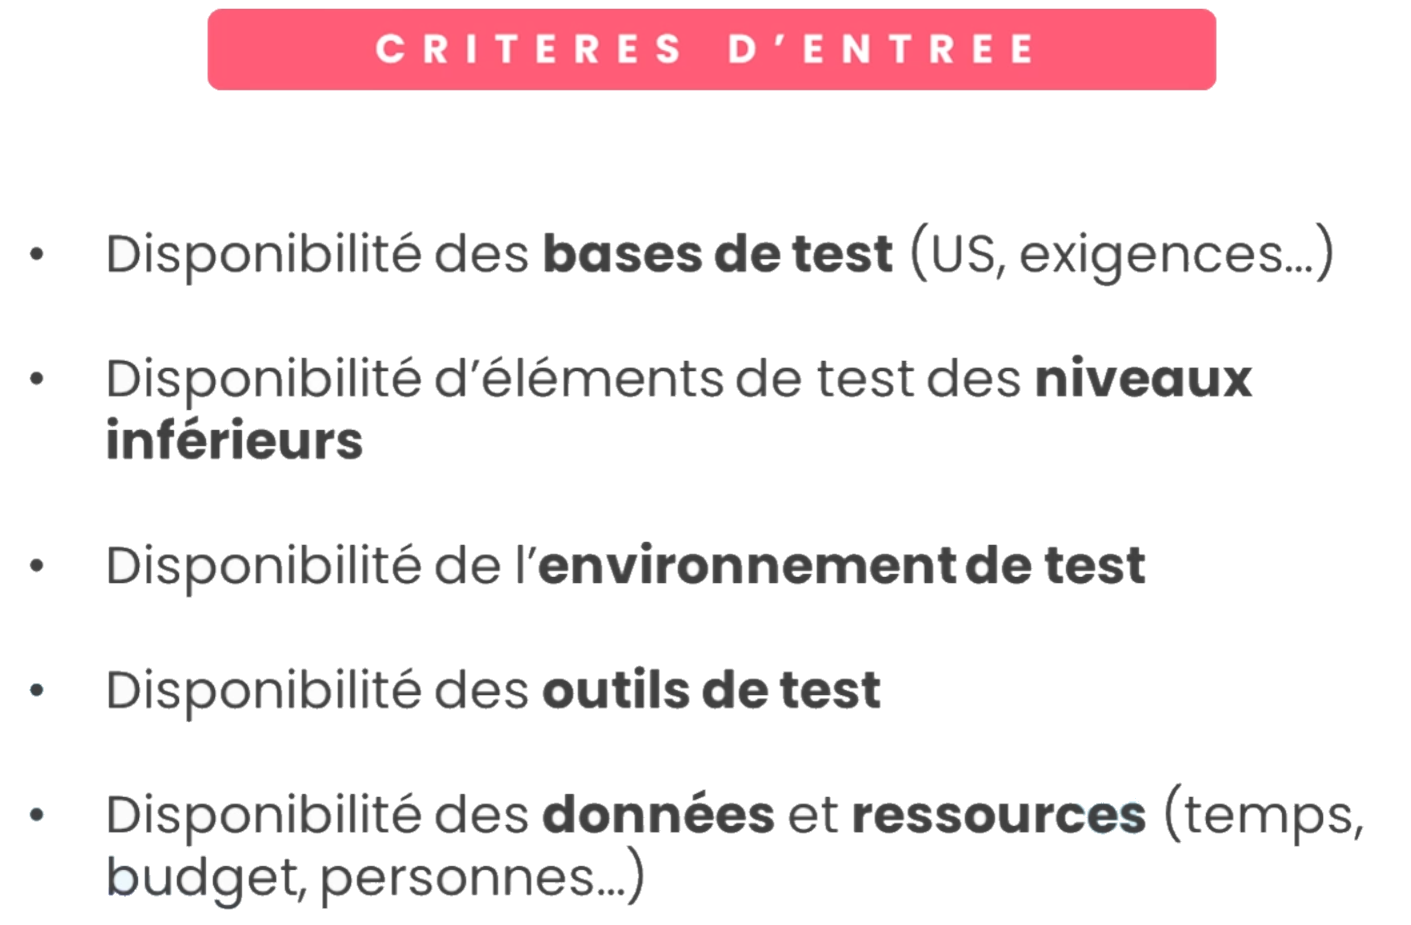
\includegraphics[width=0.9\textwidth]{images/Criteres_ES_02.png}
        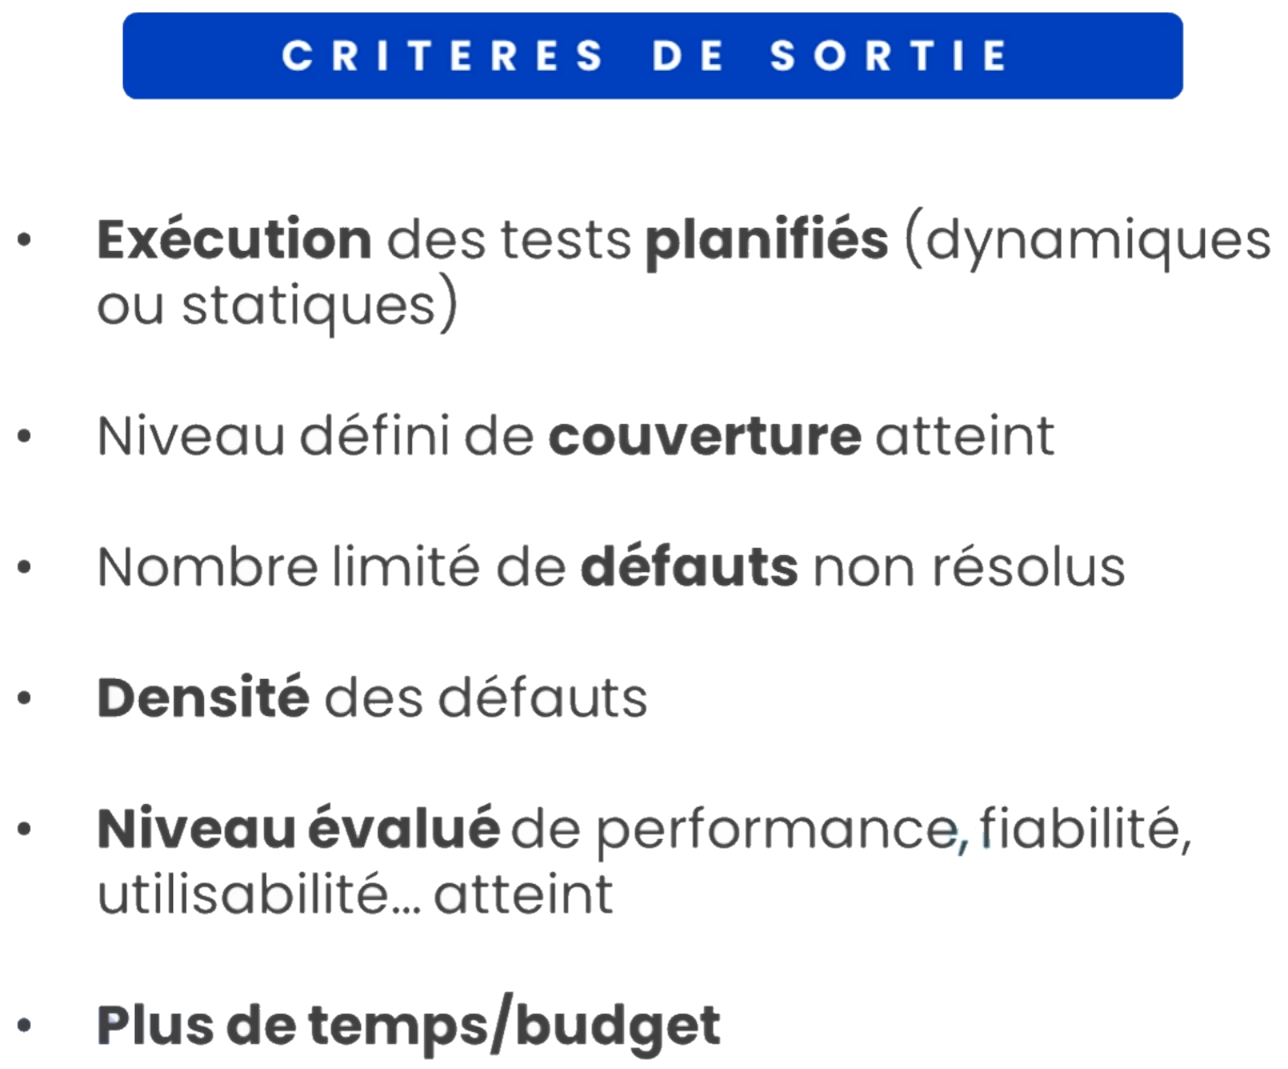
\includegraphics[width=0.9\textwidth]{images/Criteres_ES_03.png}
    \end{center}
    
	\subsection{L'estimation de l'effort}

    \begin{center}
        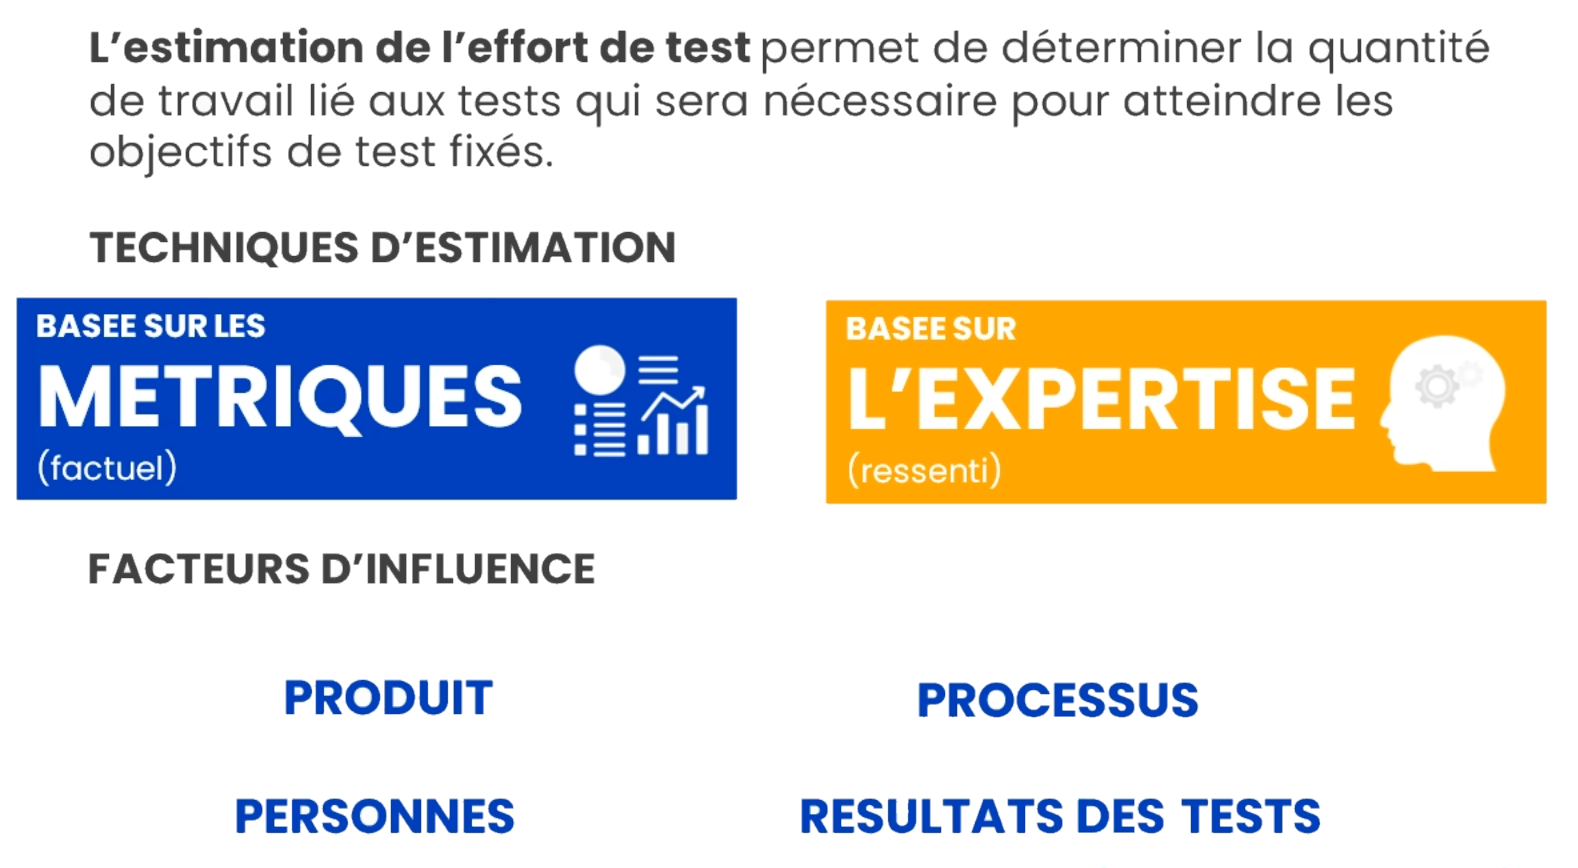
\includegraphics[width=0.9\textwidth]{images/estim_effort_01.png}
        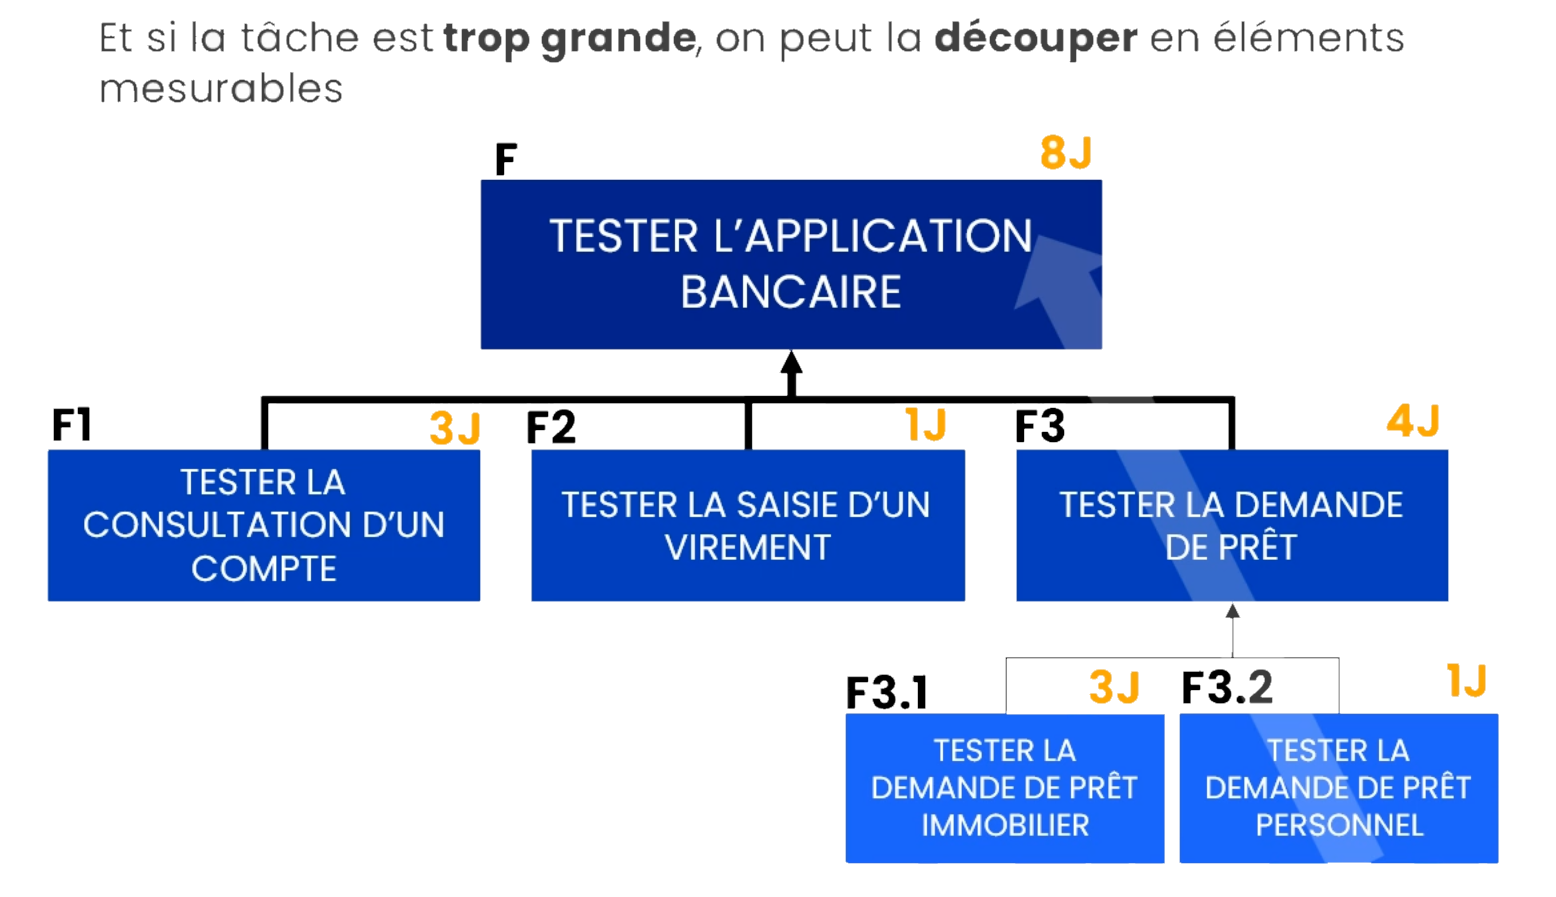
\includegraphics[width=0.9\textwidth]{images/estim_effort_02.png}
    \end{center}
    
	\subsection{Les ratios}

    \begin{center}
        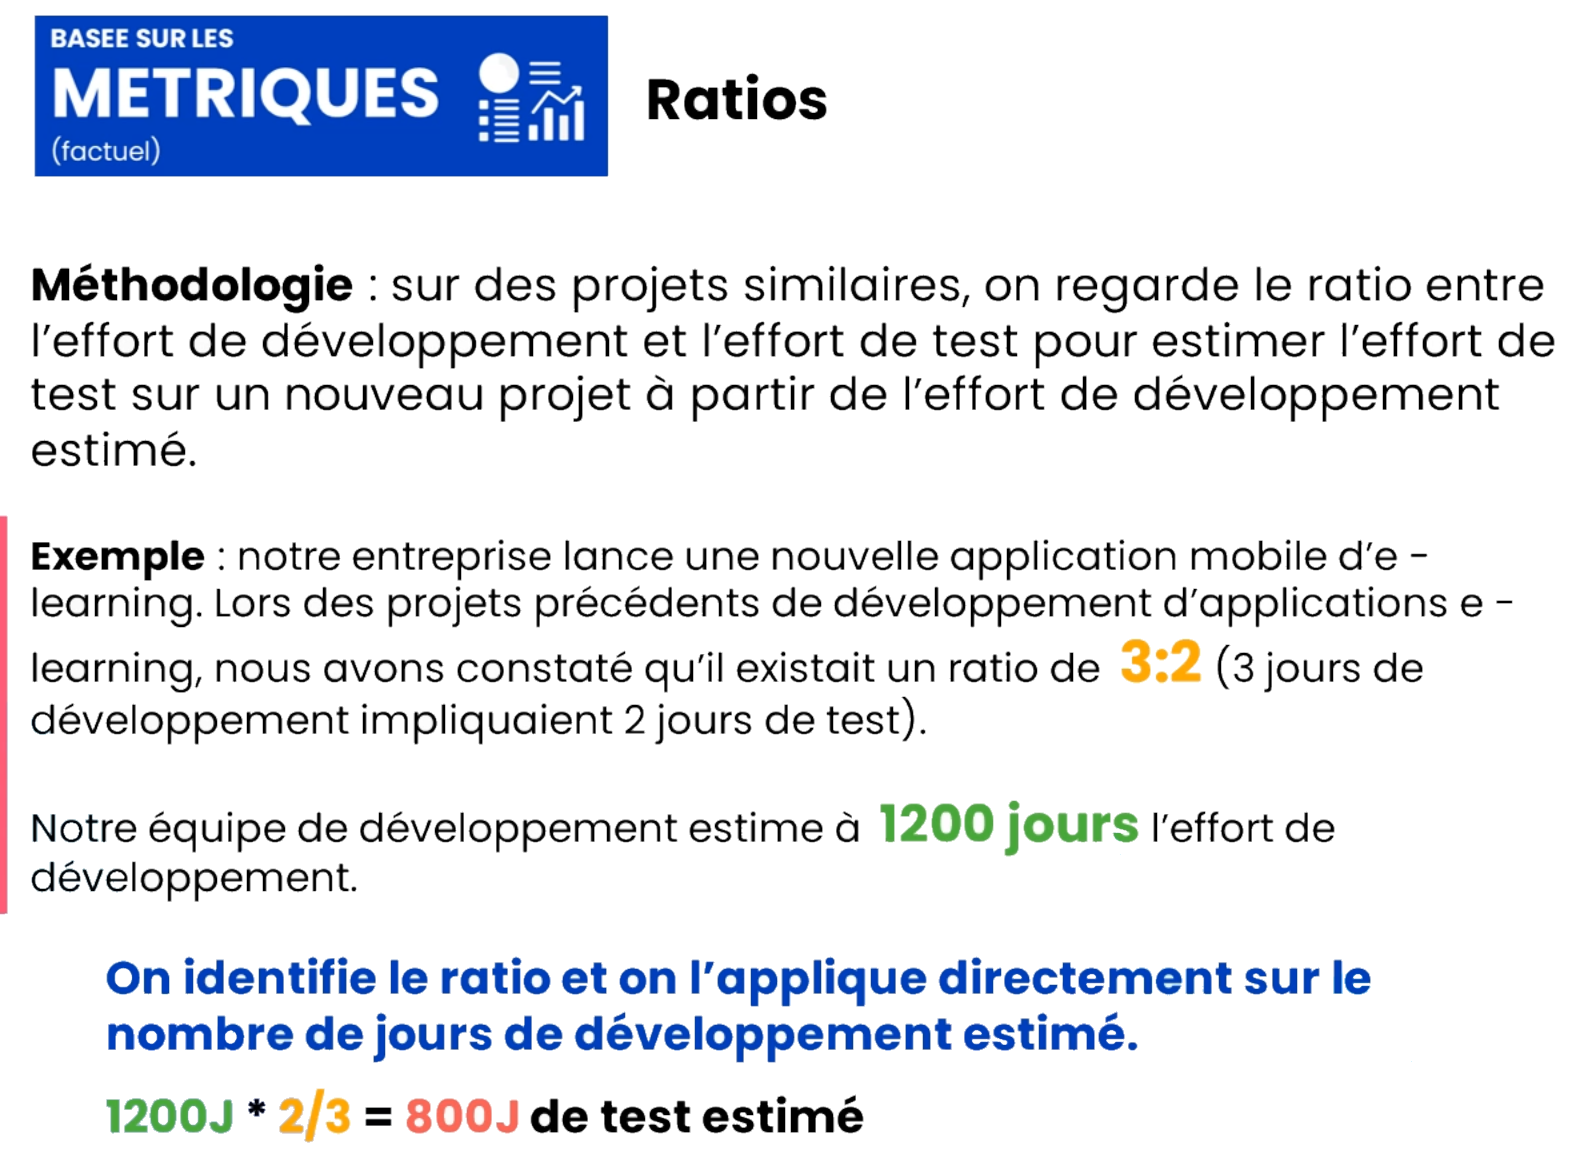
\includegraphics[width=0.9\textwidth]{images/ratios_01.png}
        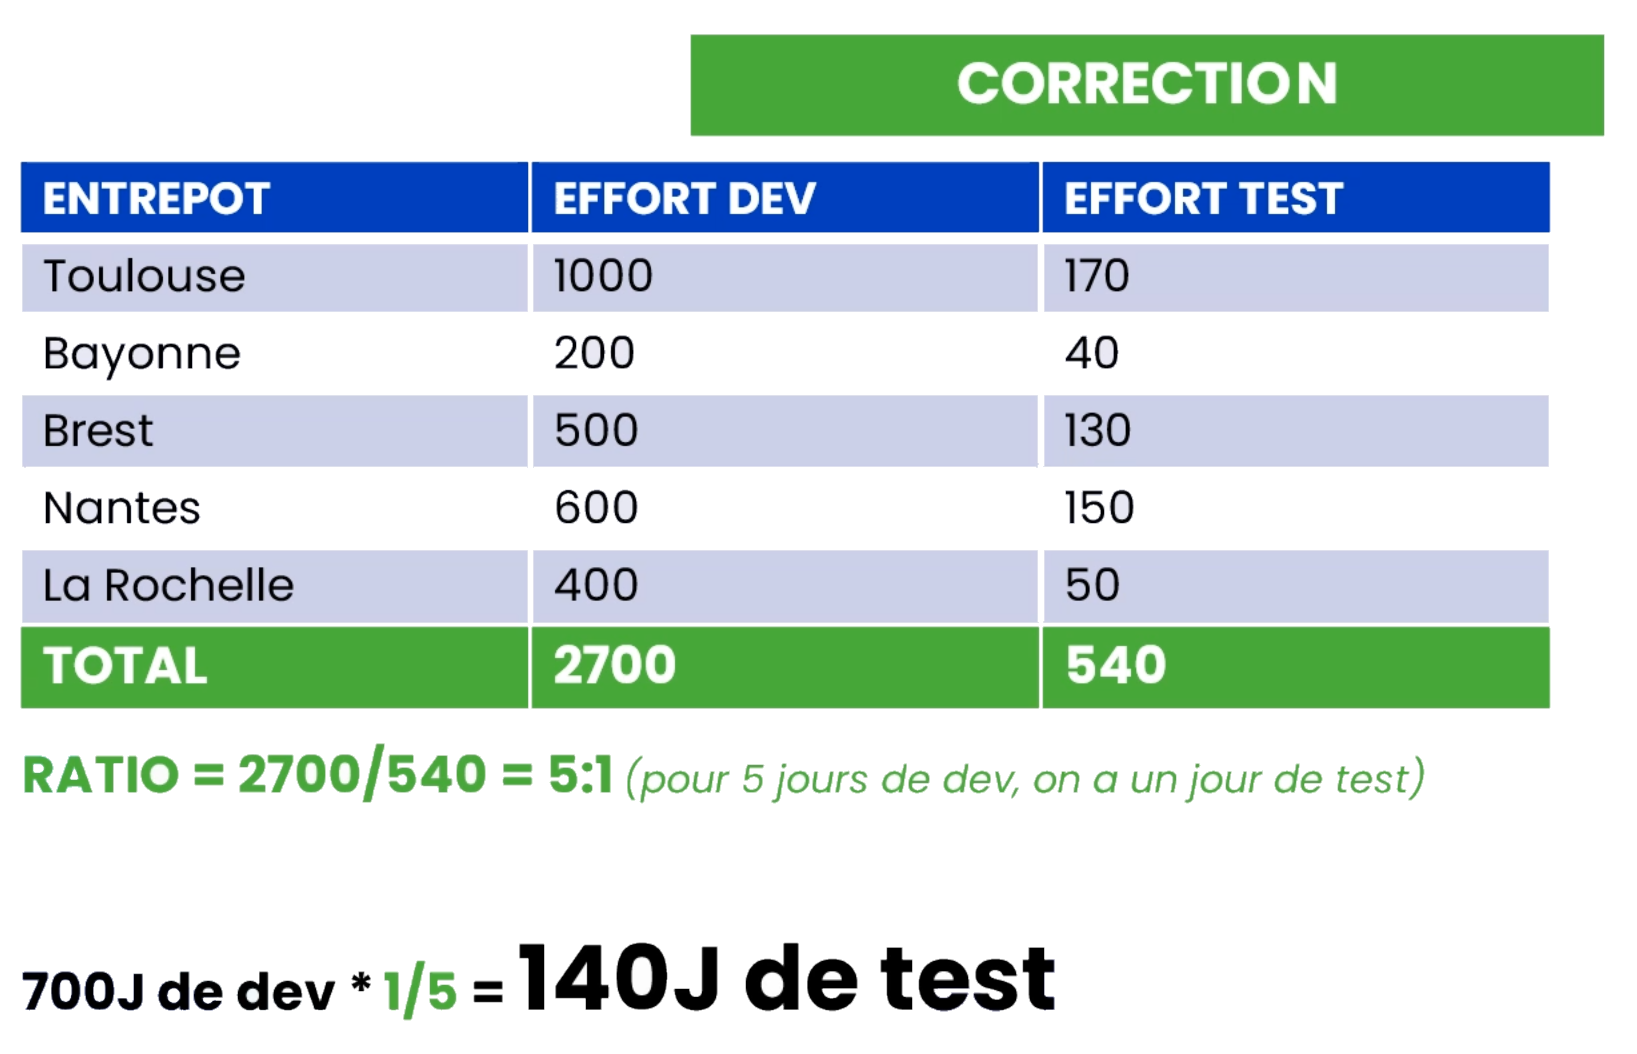
\includegraphics[width=0.9\textwidth]{images/ratios_02.png}
    \end{center}
    
	\subsection{L'extrapolation}

    \begin{center}
        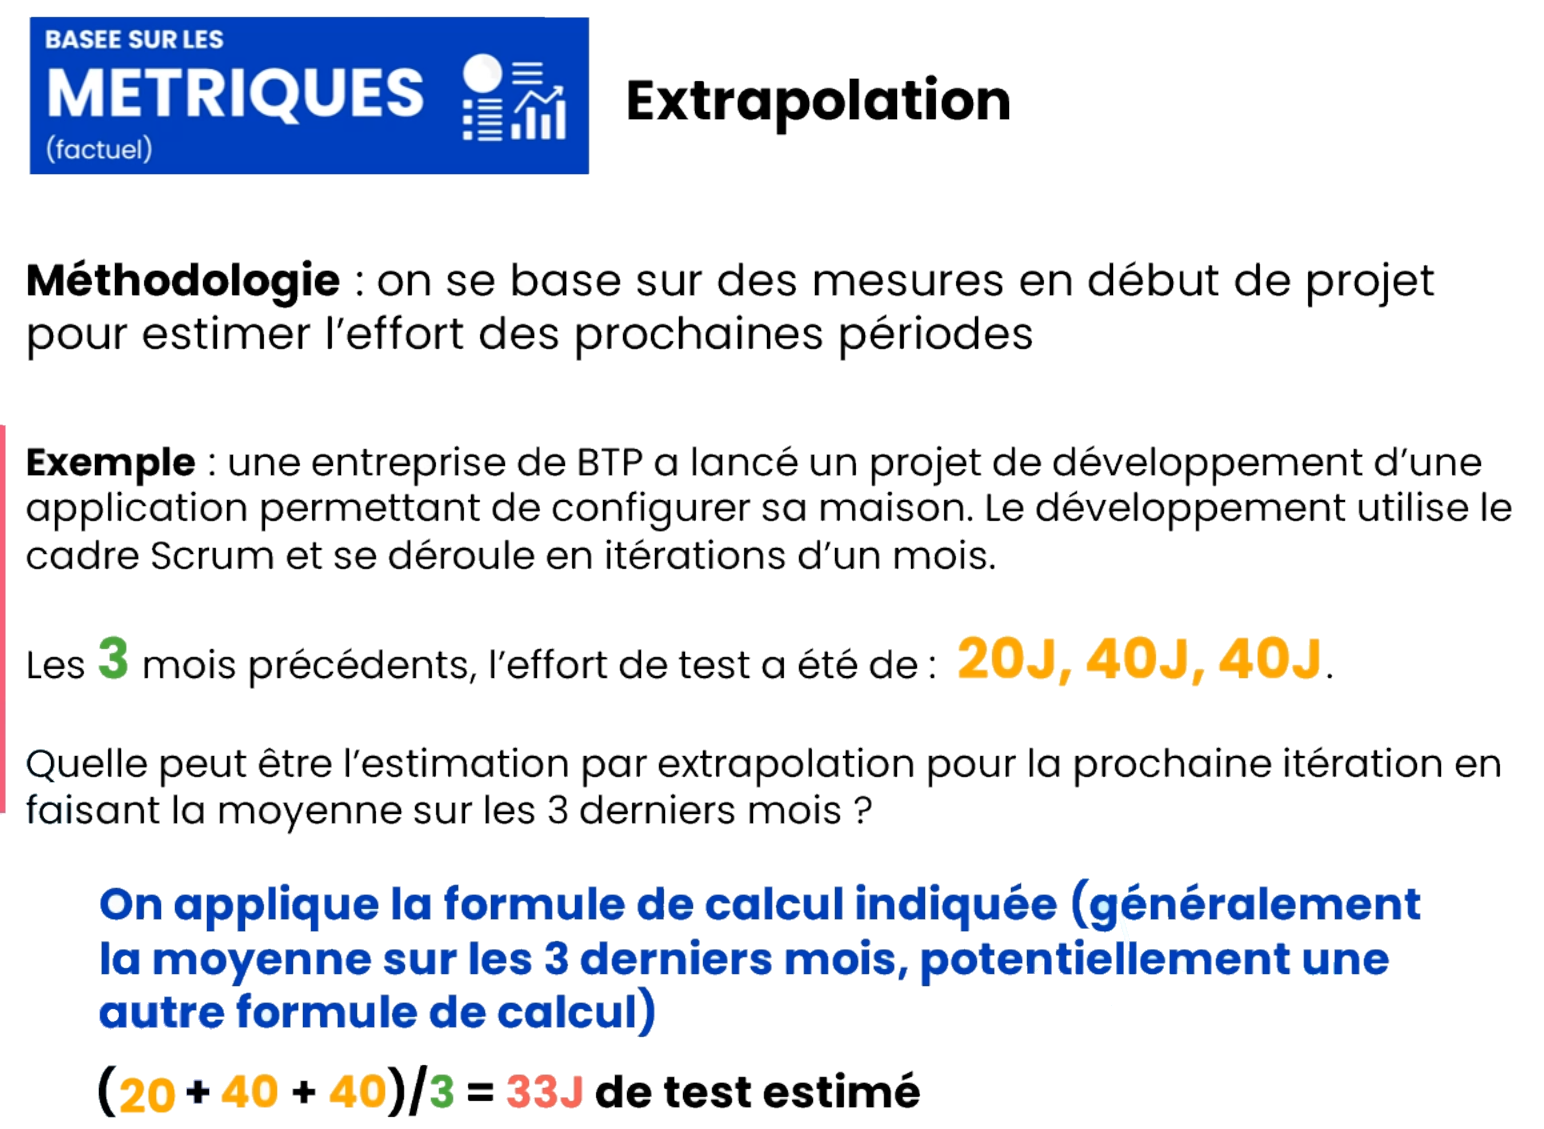
\includegraphics[width=0.9\textwidth]{images/extrapolation_01.png}
        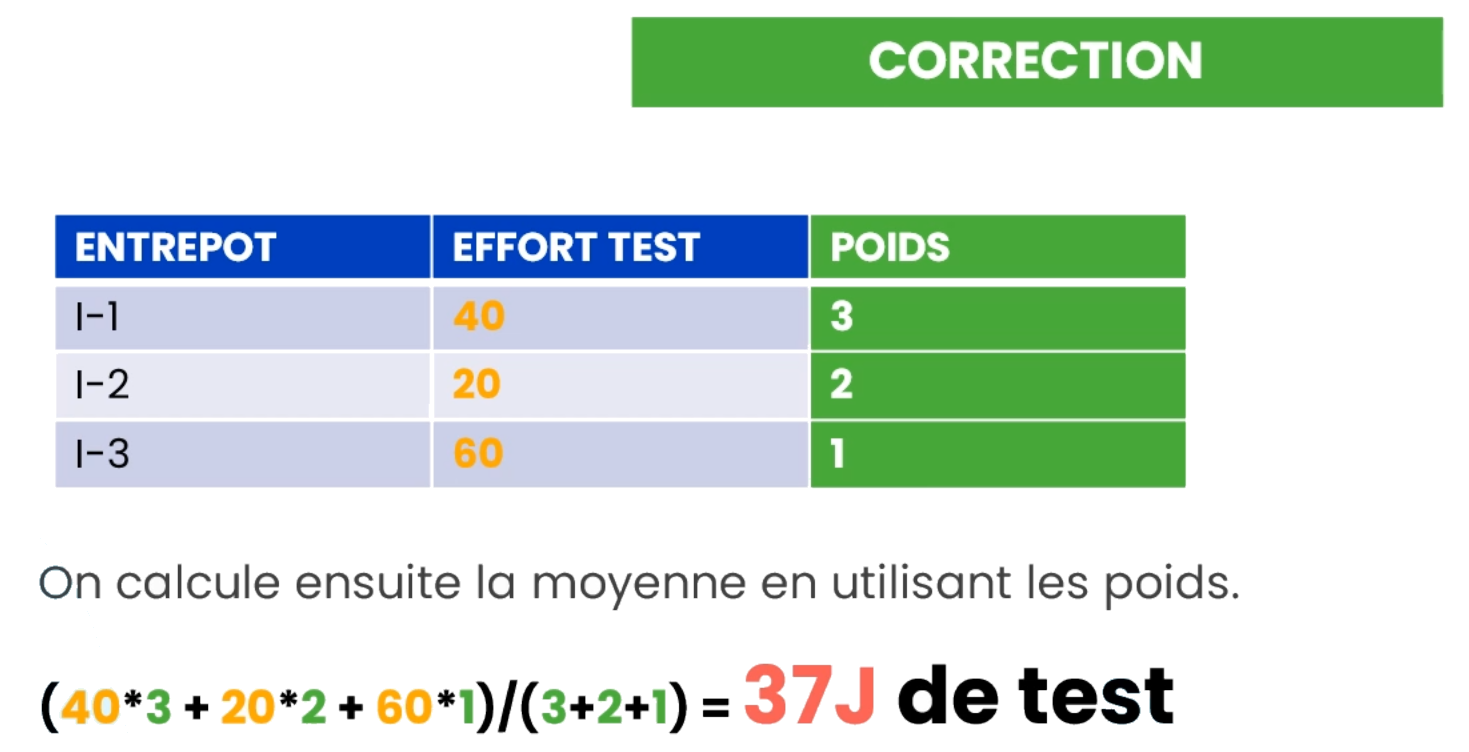
\includegraphics[width=0.9\textwidth]{images/extrapolation_02.png}
    \end{center}
    
	\subsection{La méthode Wideband Delphi}

    \begin{center}
        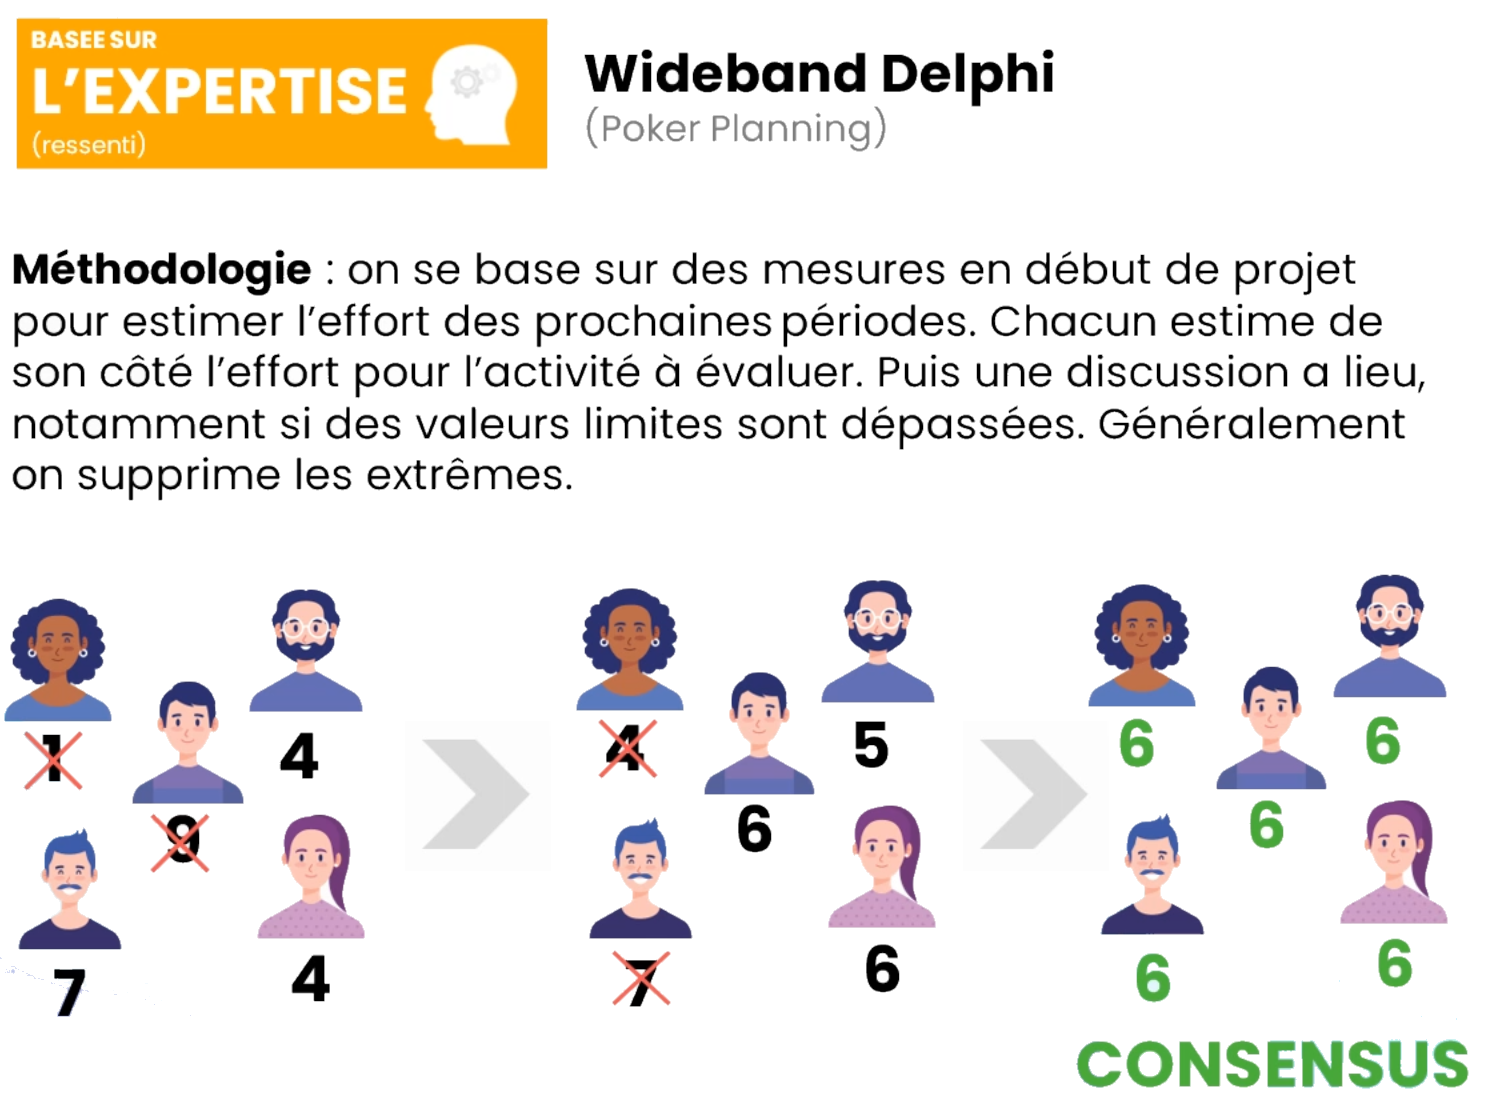
\includegraphics[width=0.9\textwidth]{images/wideband_delphi_01.png}
        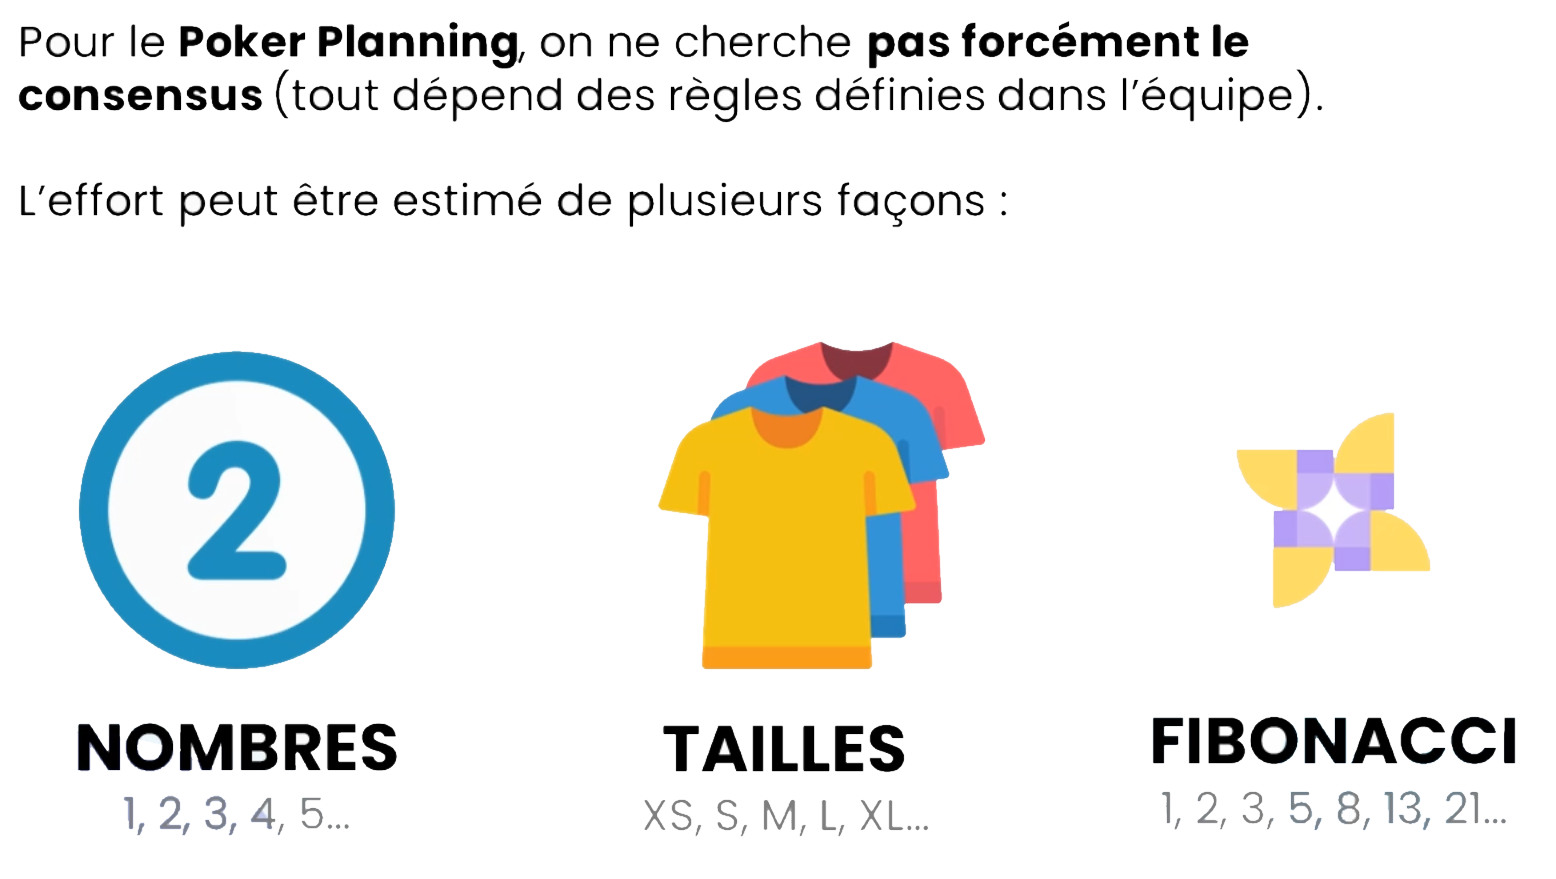
\includegraphics[width=0.9\textwidth]{images/wideband_delphi_02.png}
    \end{center}
    
	\subsection{La méthode des 3 Points}

    \begin{center}
        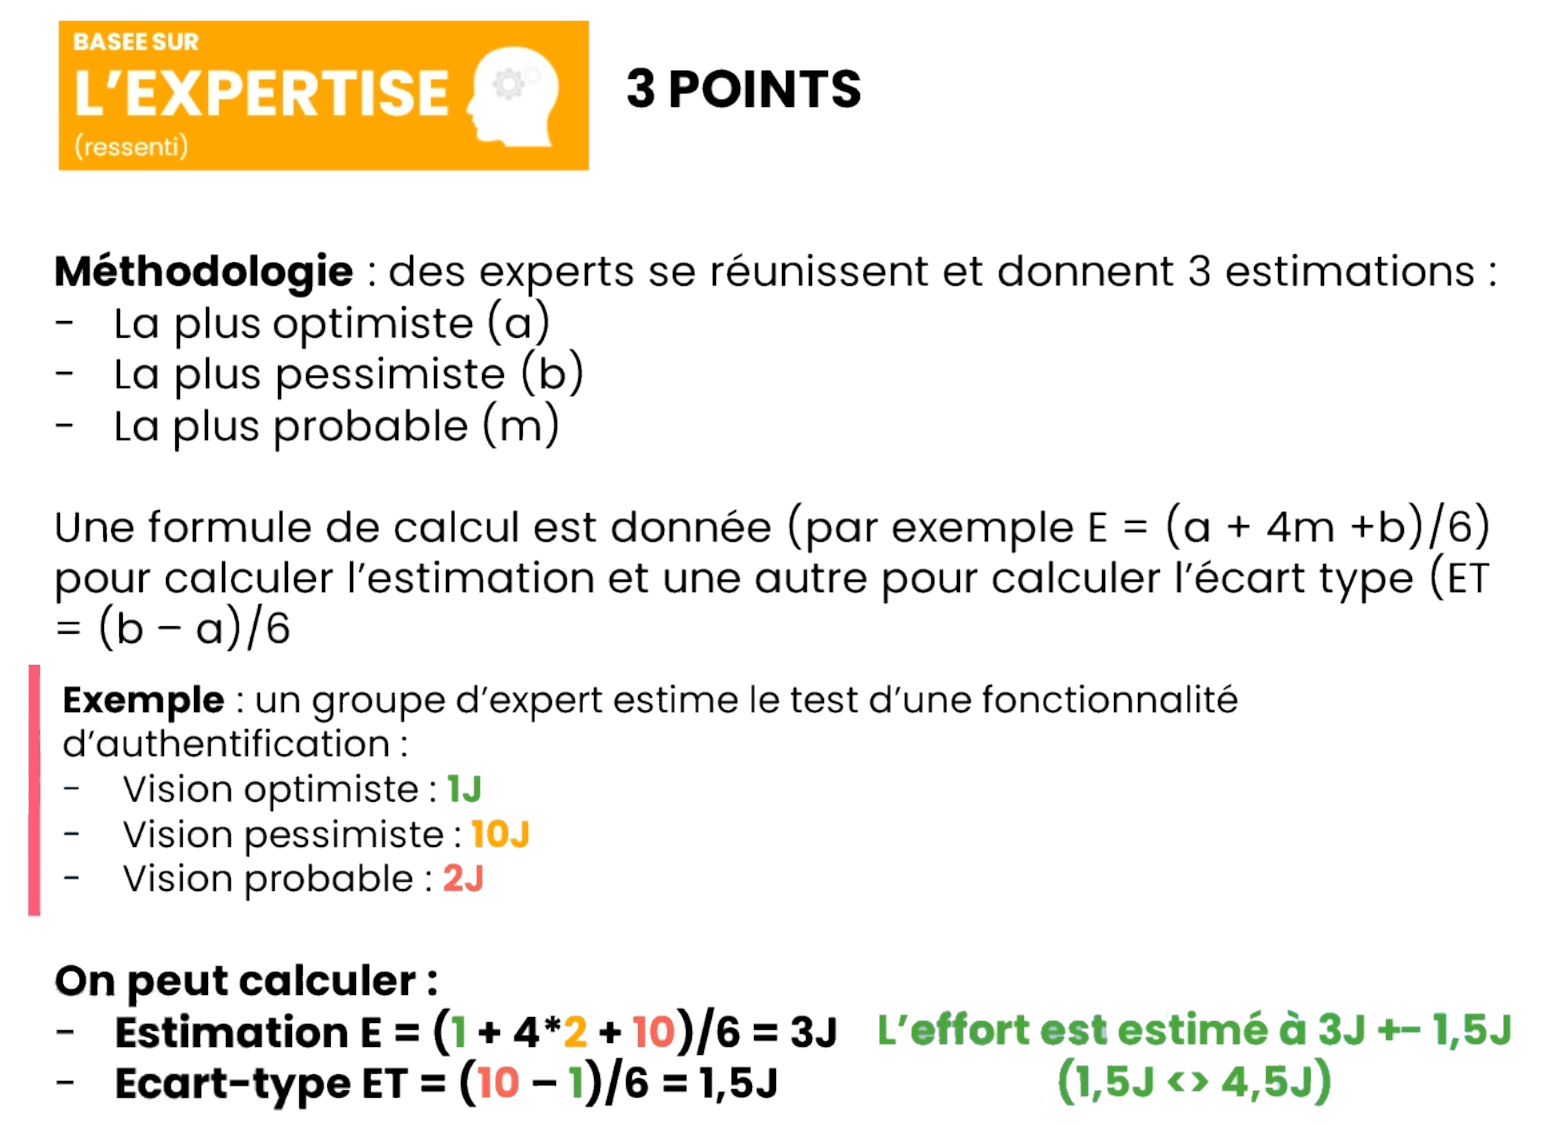
\includegraphics[width=0.9\textwidth]{images/3_points_01.png}
        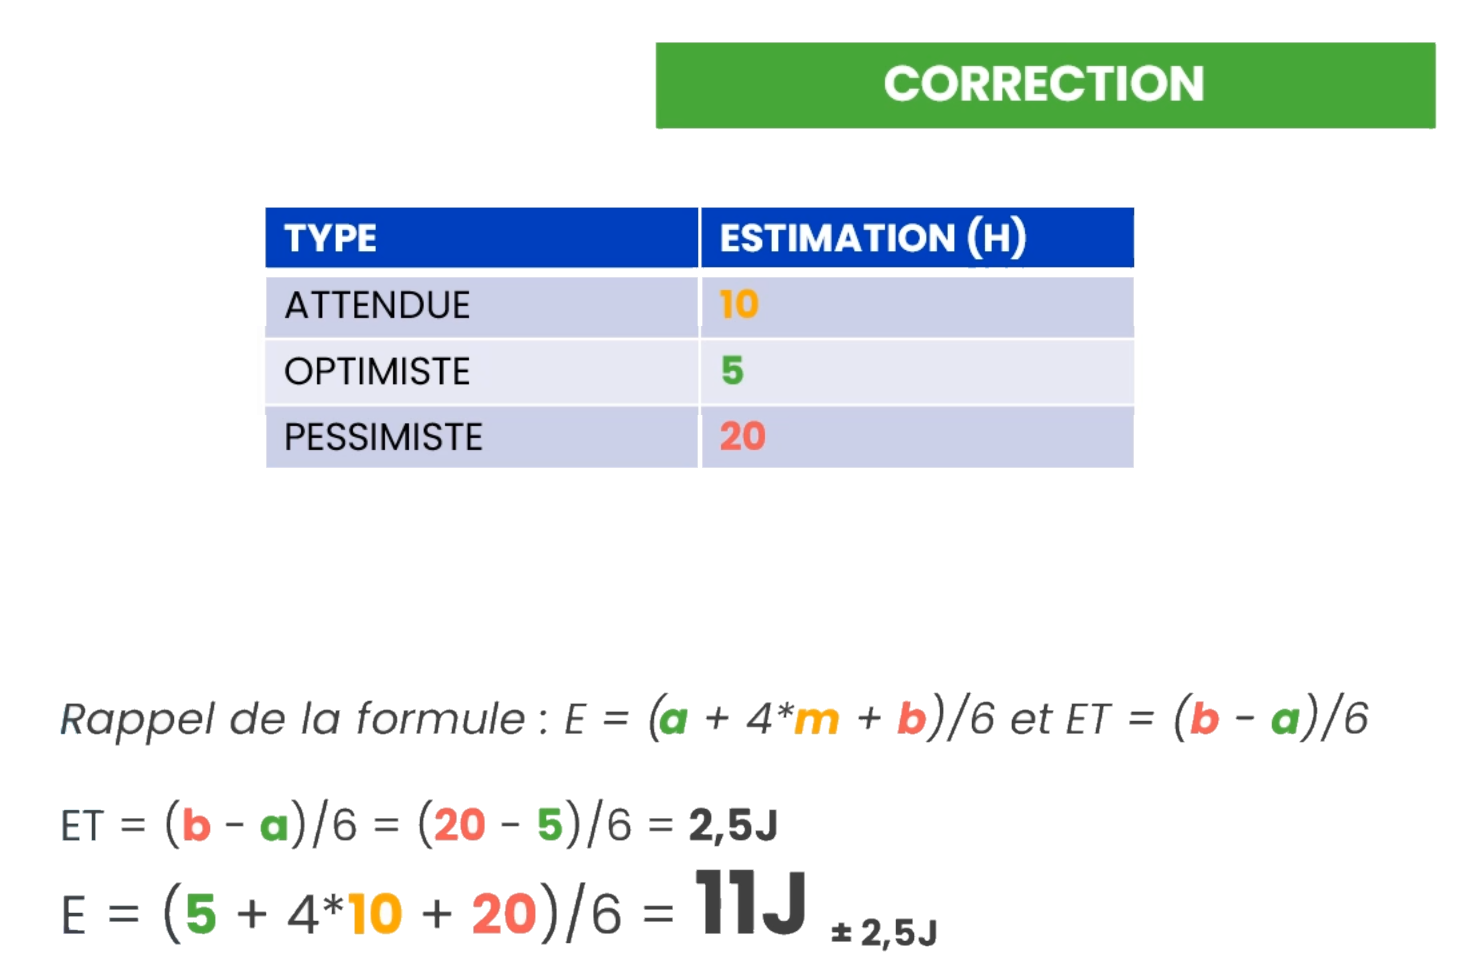
\includegraphics[width=0.9\textwidth]{images/3_points_02.png}
    \end{center}
    
	\subsection{La priorisation}

    \begin{center}
        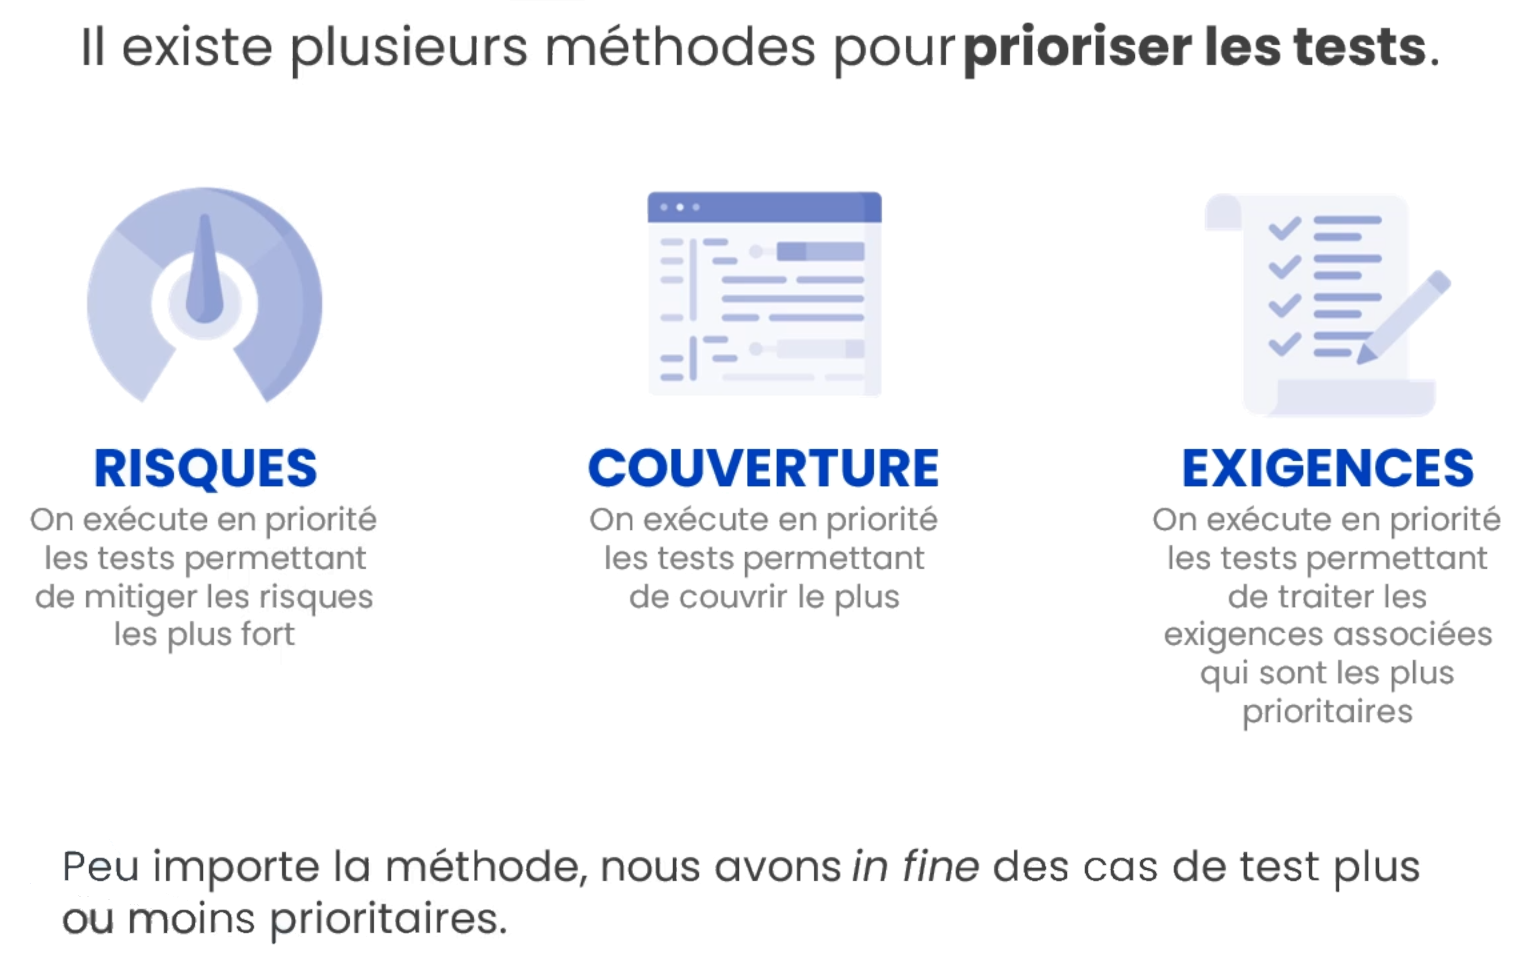
\includegraphics[width=0.9\textwidth]{images/priori_01.png}
        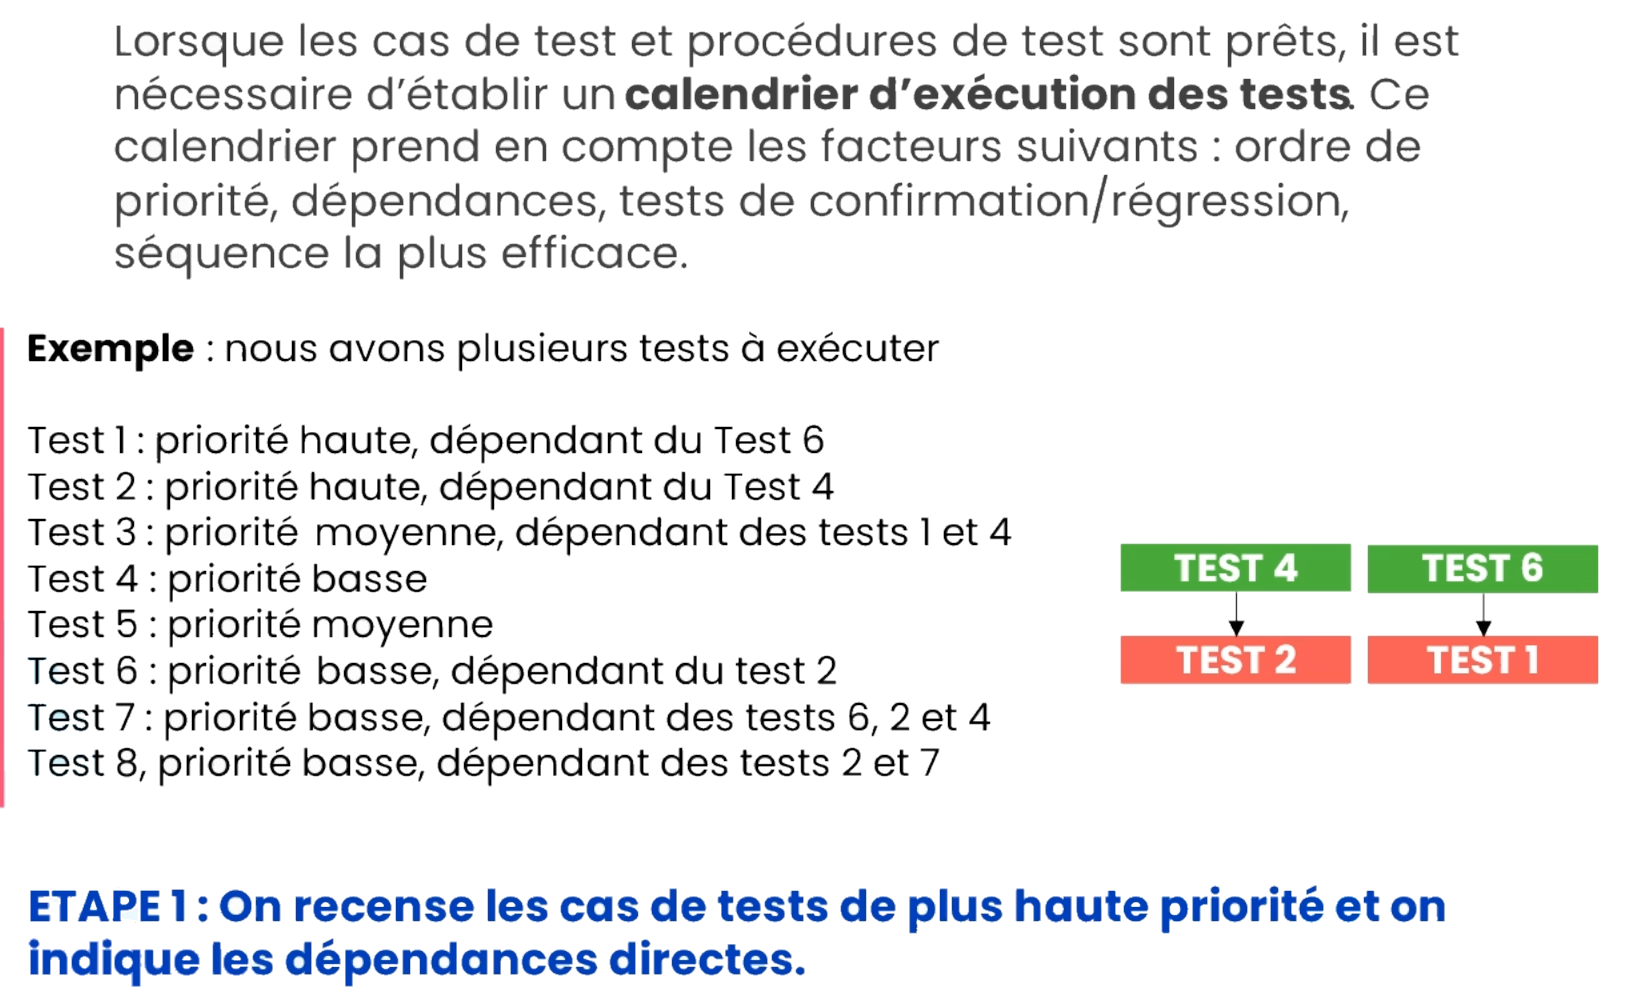
\includegraphics[width=0.9\textwidth]{images/priori_02.png}
        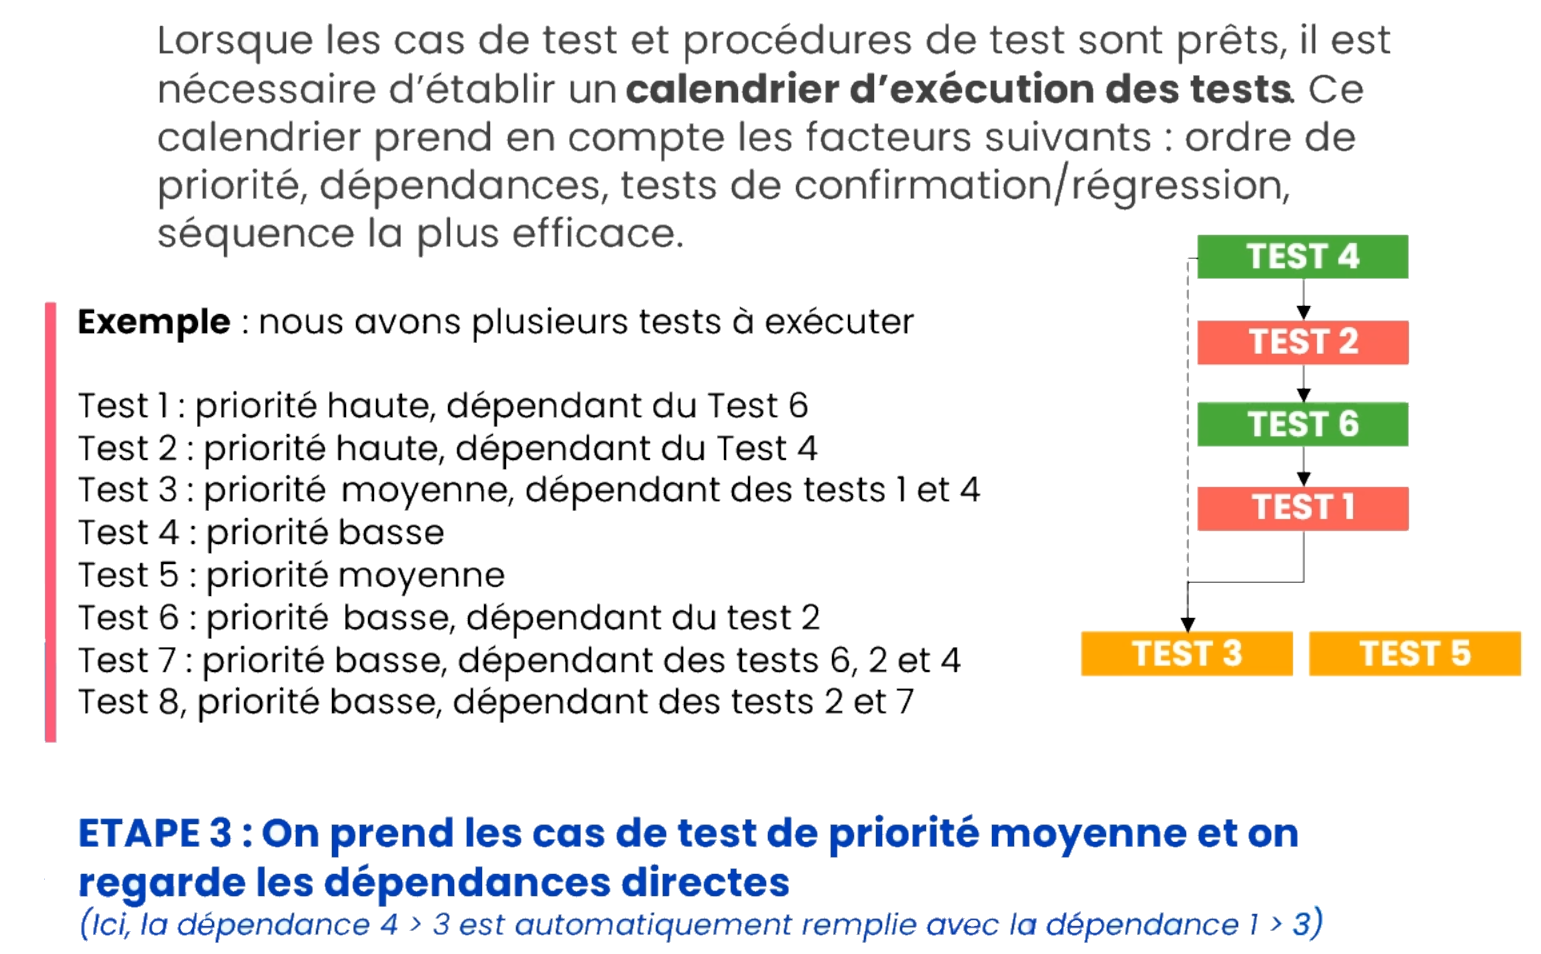
\includegraphics[width=0.9\textwidth]{images/priori_03.png}
        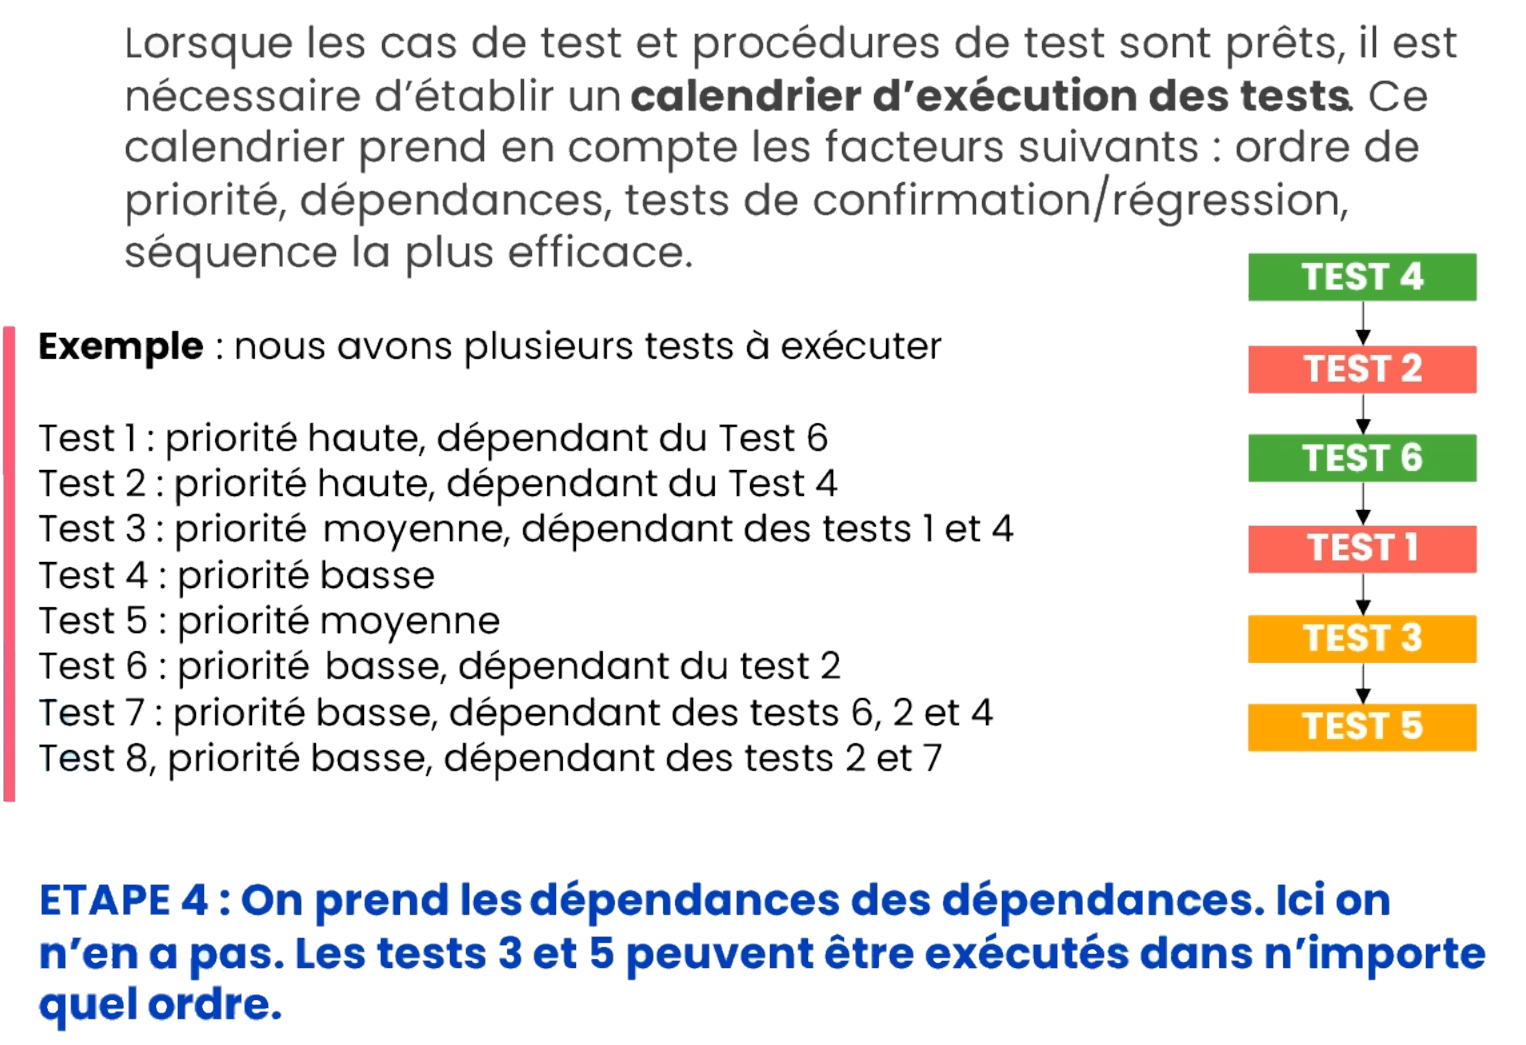
\includegraphics[width=0.9\textwidth]{images/priori_04.png}
    \end{center}
    
	\subsection{La pyramide}

    \begin{center}
        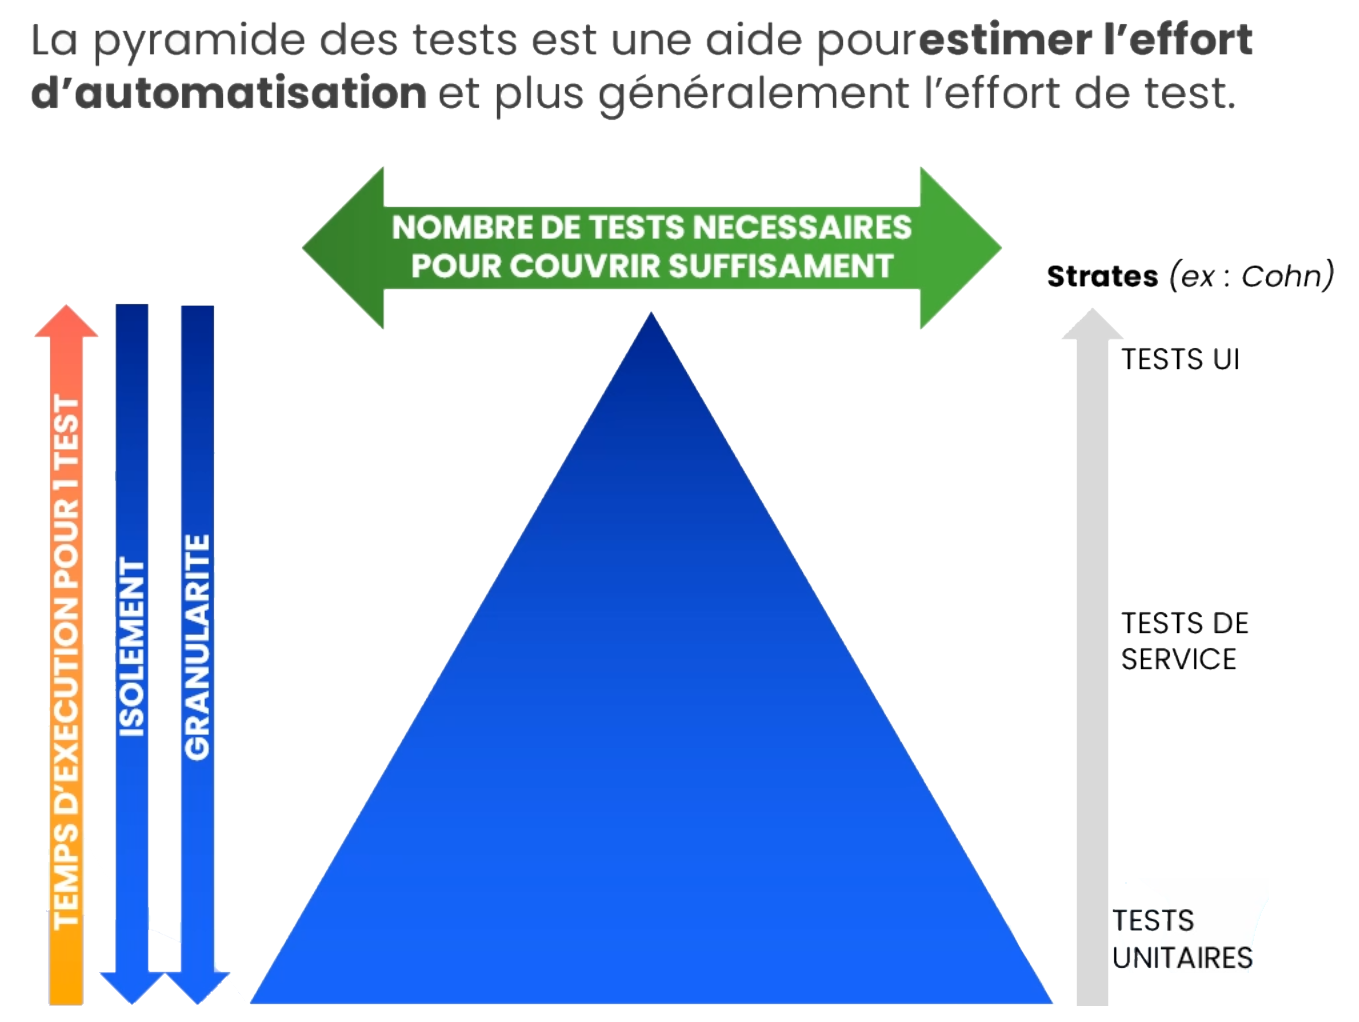
\includegraphics[width=0.9\textwidth]{images/pyramide.png}
    \end{center}
    
	\subsection{Les quadrants}

    \begin{center}
        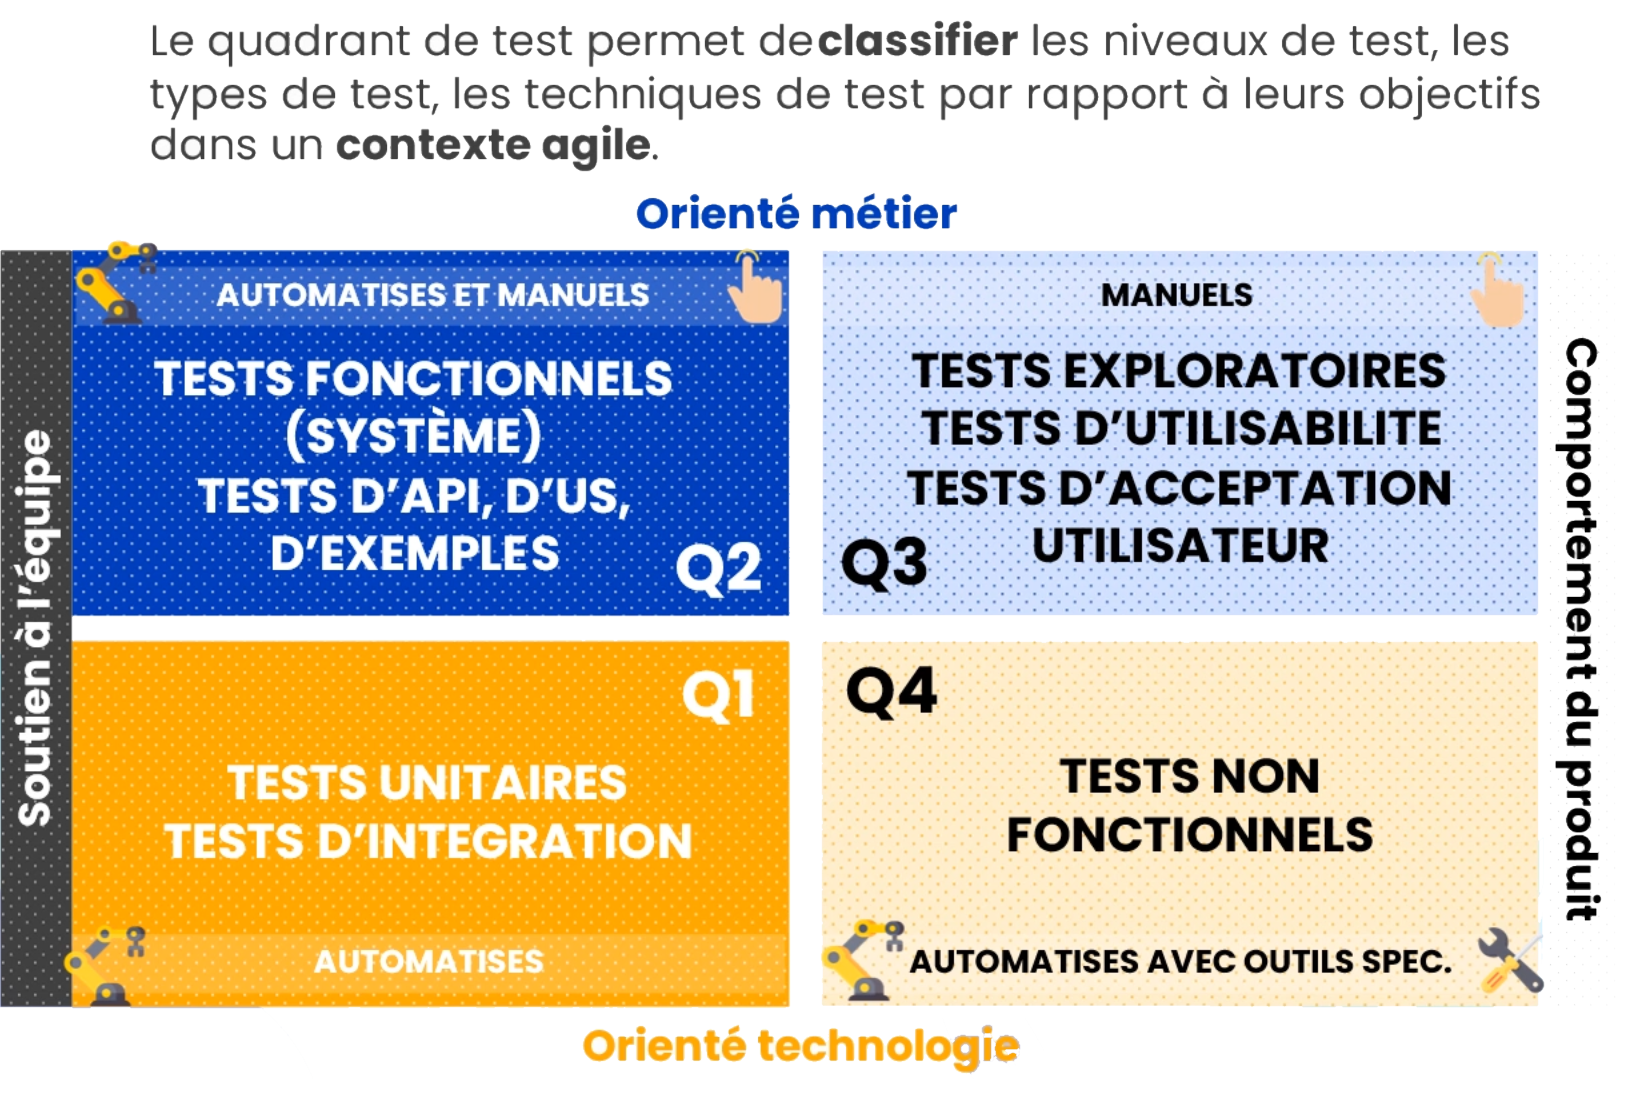
\includegraphics[width=0.9\textwidth]{images/quadrants.png}
    \end{center}
    
	\subsection{L'analyse du risque}

    \begin{center}
        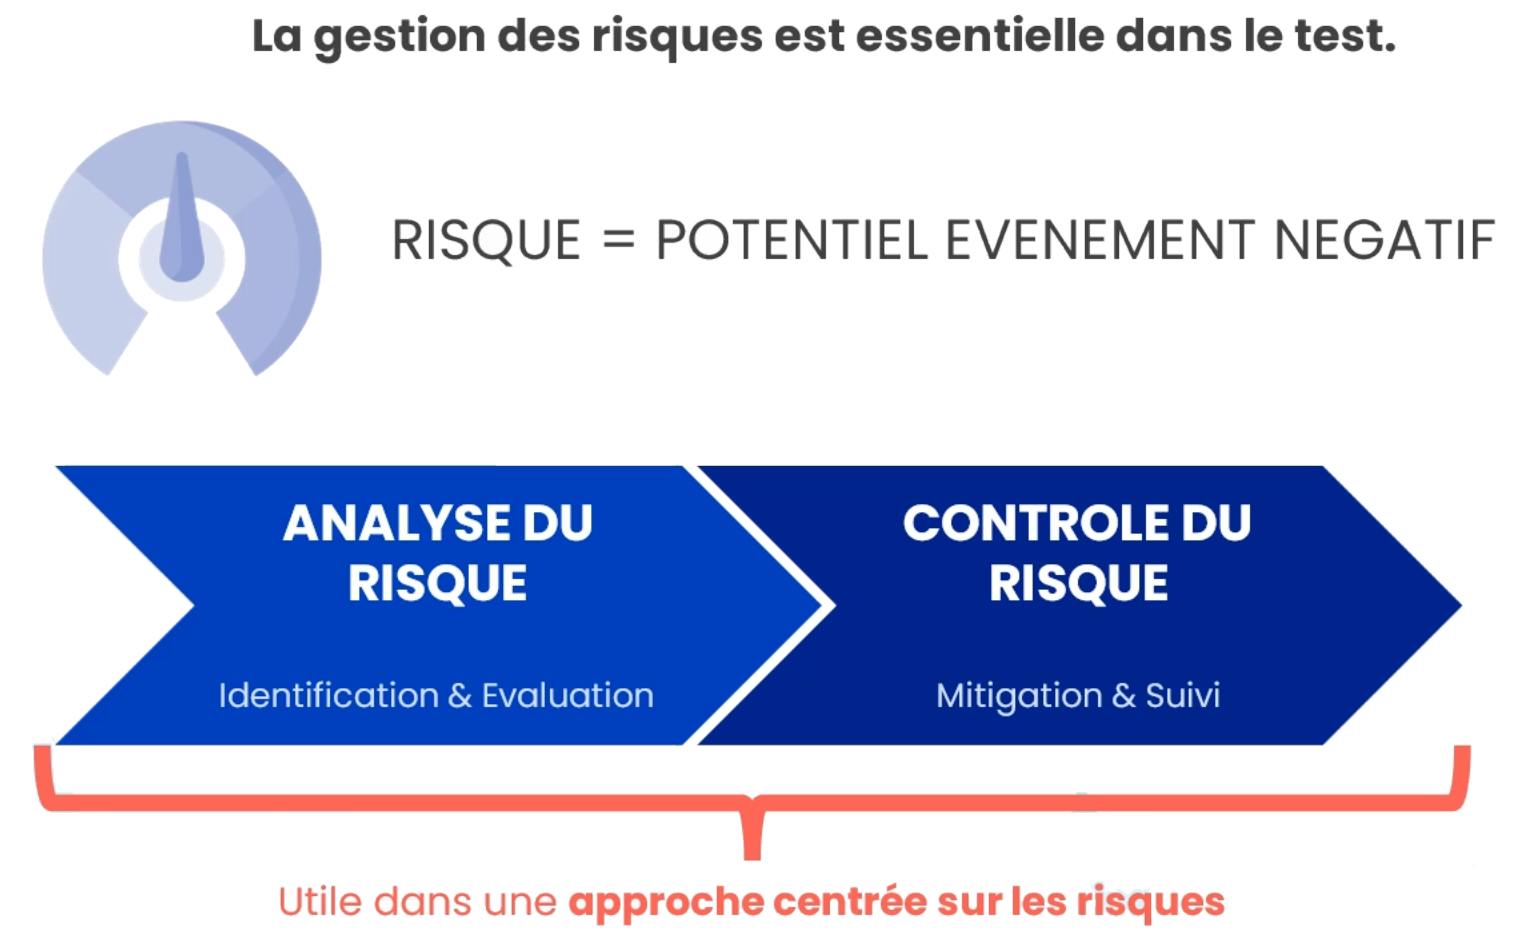
\includegraphics[width=0.9\textwidth]{images/analyse_risque_01.png}
        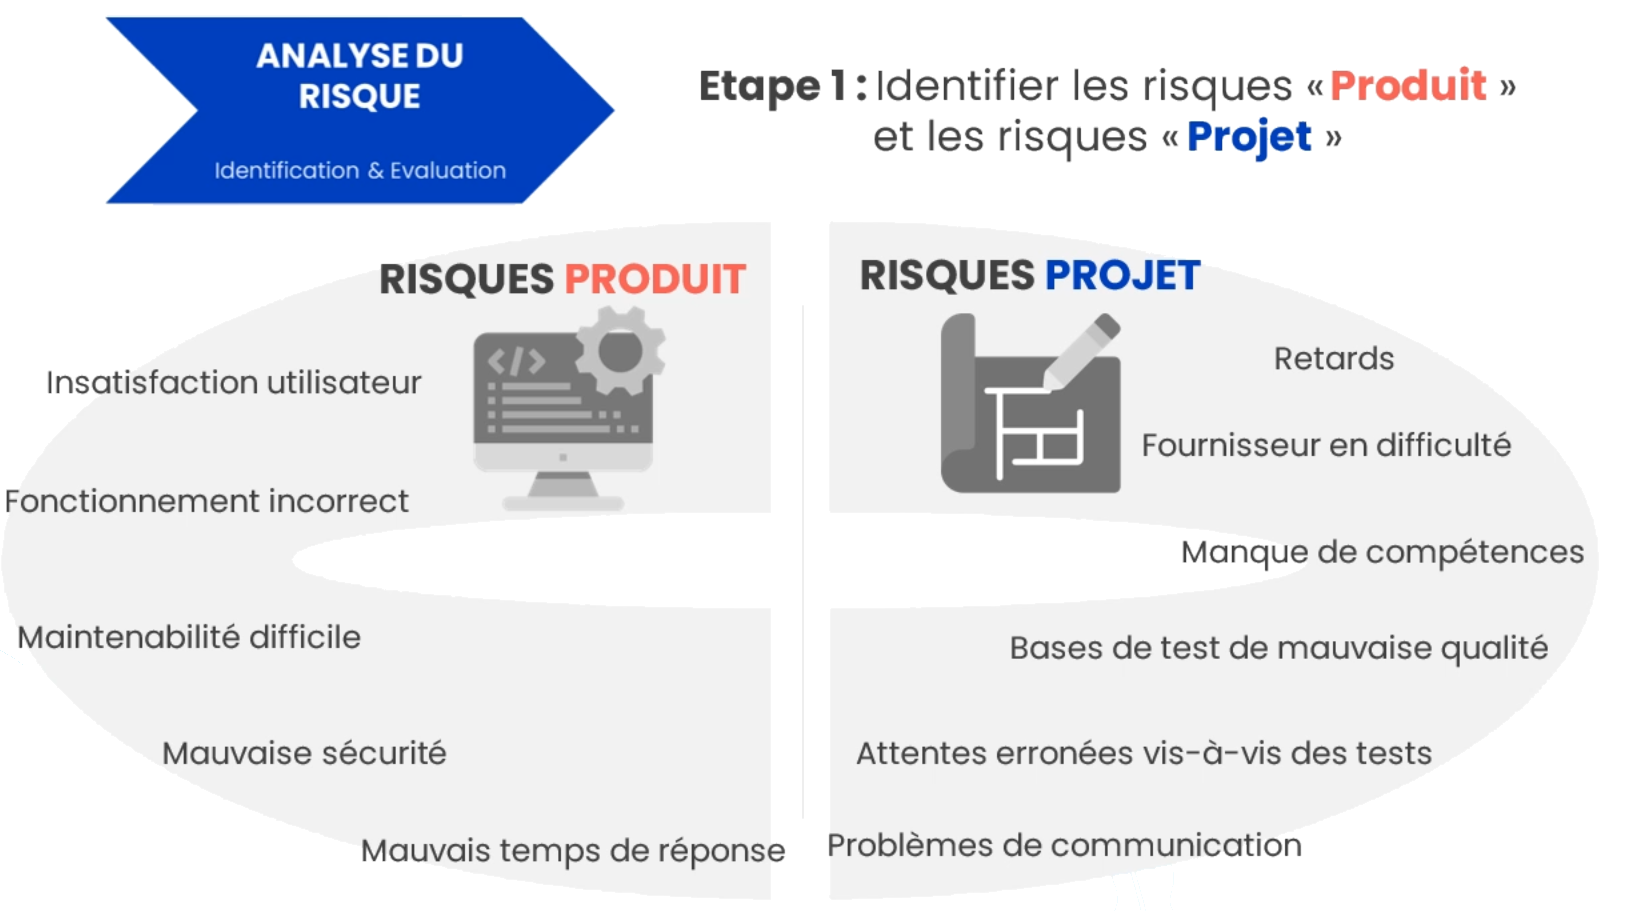
\includegraphics[width=0.9\textwidth]{images/analyse_risque_02.png}
        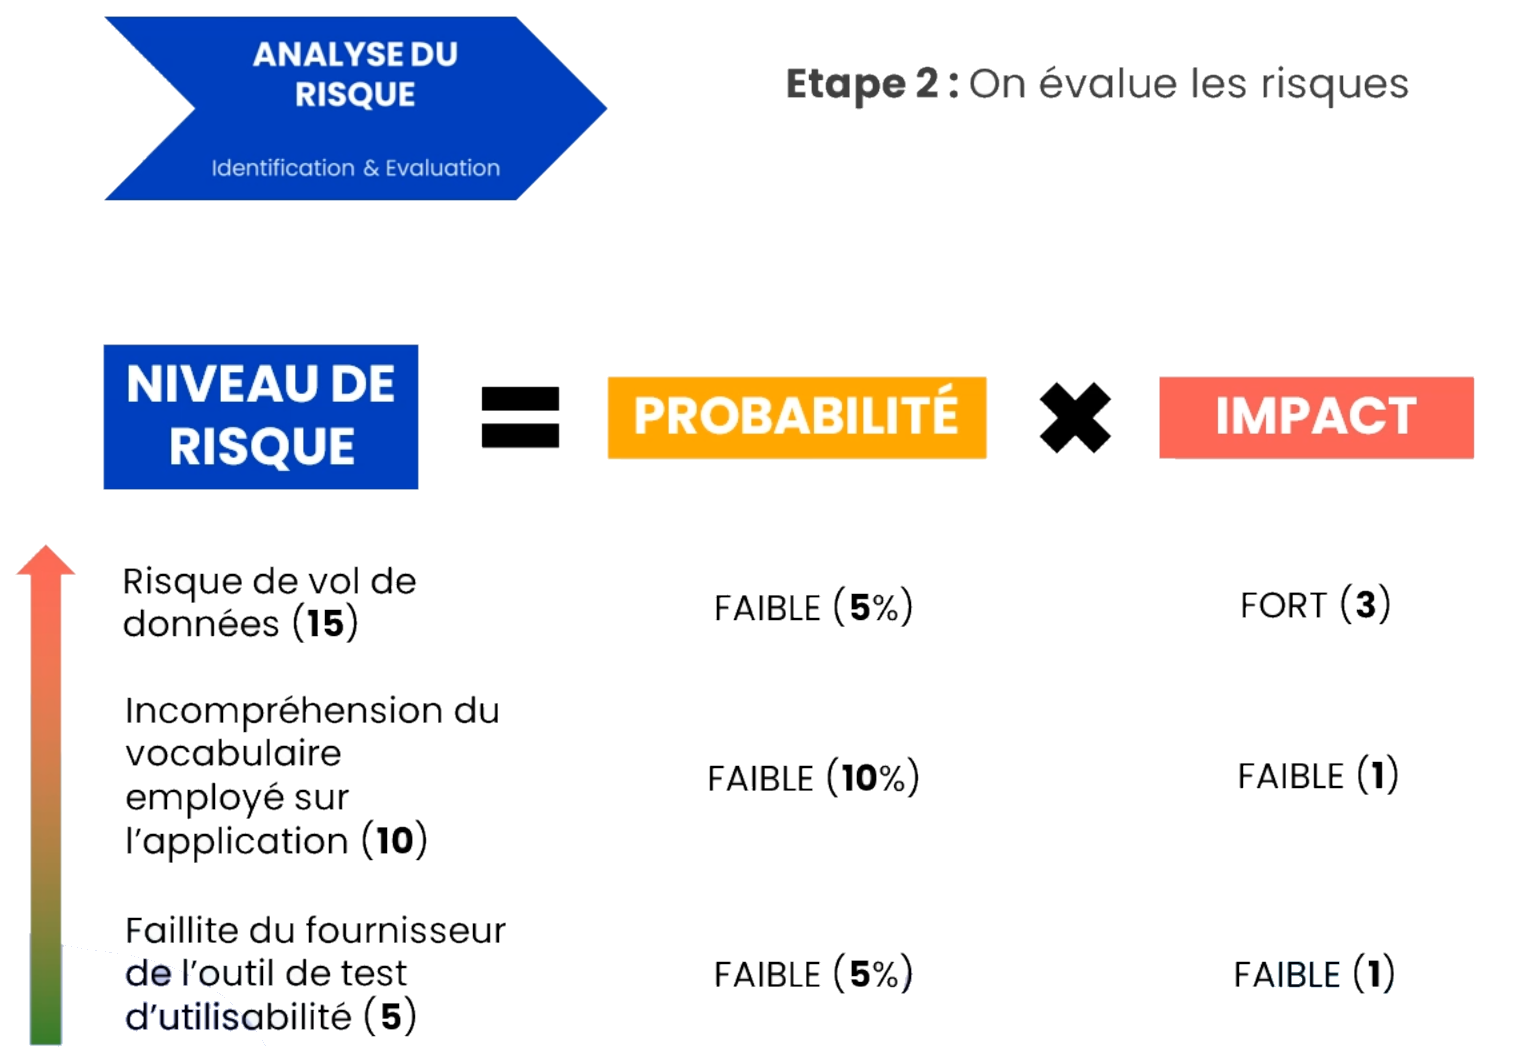
\includegraphics[width=0.9\textwidth]{images/analyse_risque_03.png}
        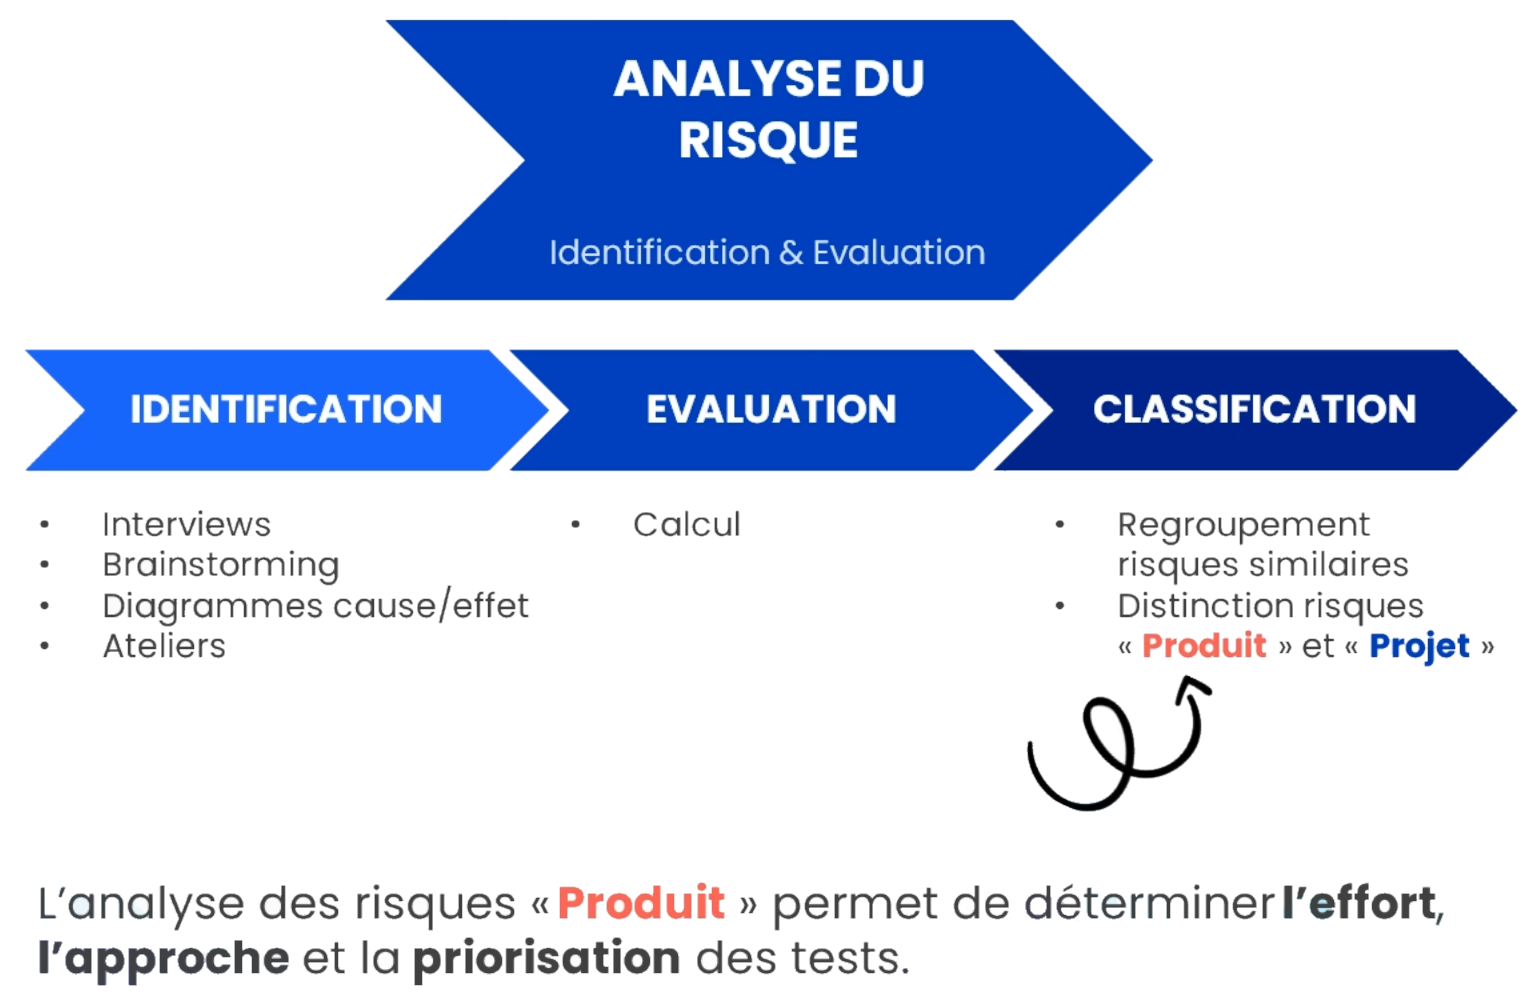
\includegraphics[width=0.9\textwidth]{images/analyse_risque_04.png}
    \end{center}

	\subsection{Le contrôle du risque}

    \begin{center}
        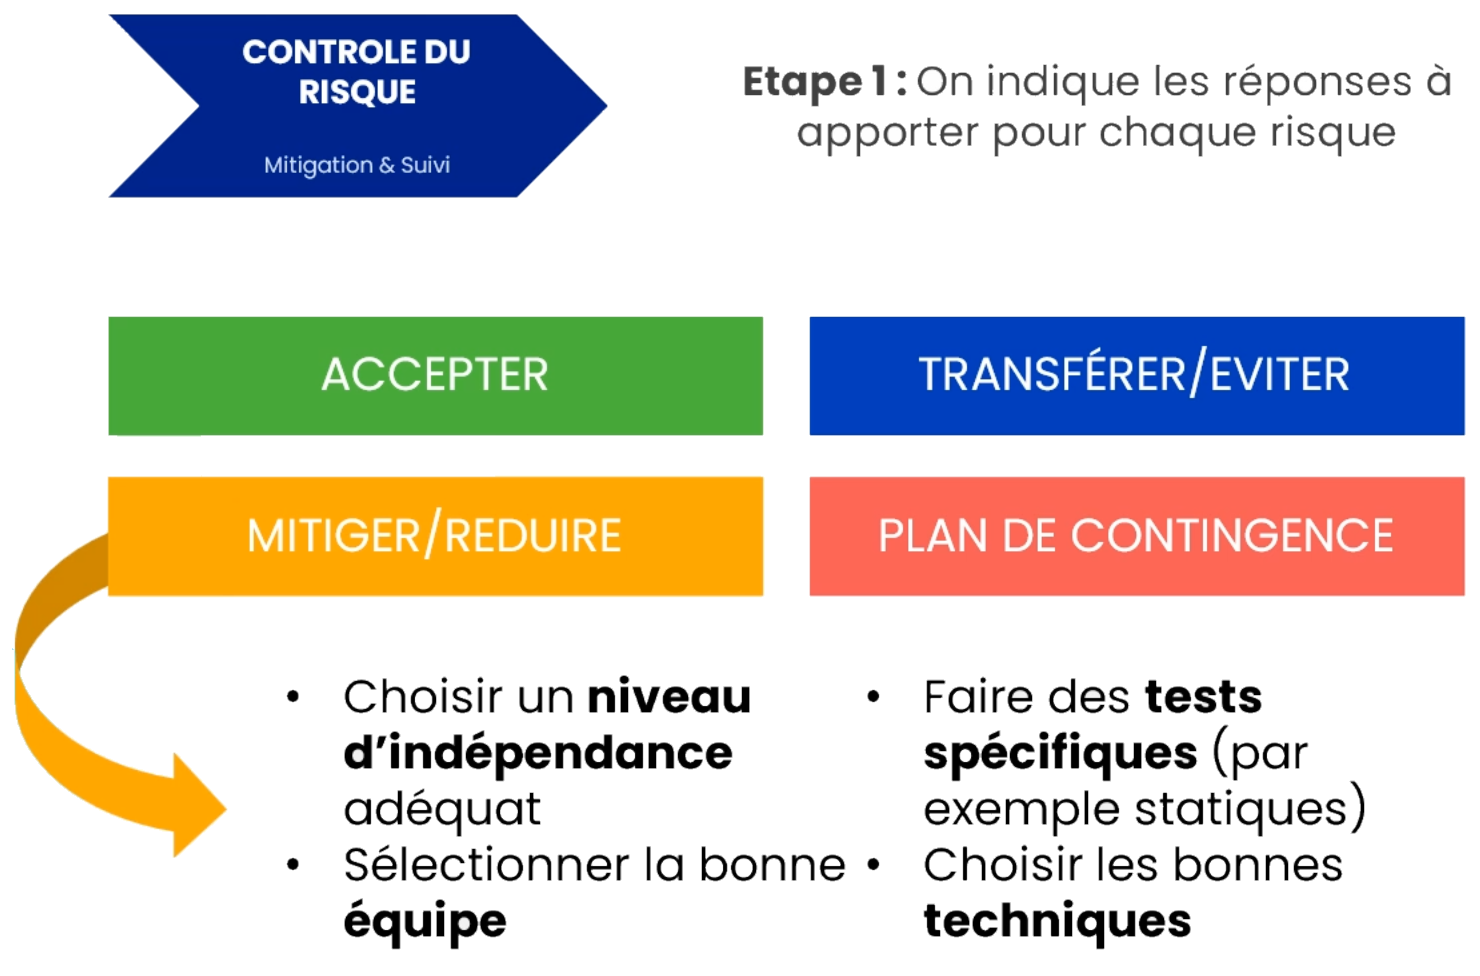
\includegraphics[width=0.9\textwidth]{images/controle_risque_01.png}
        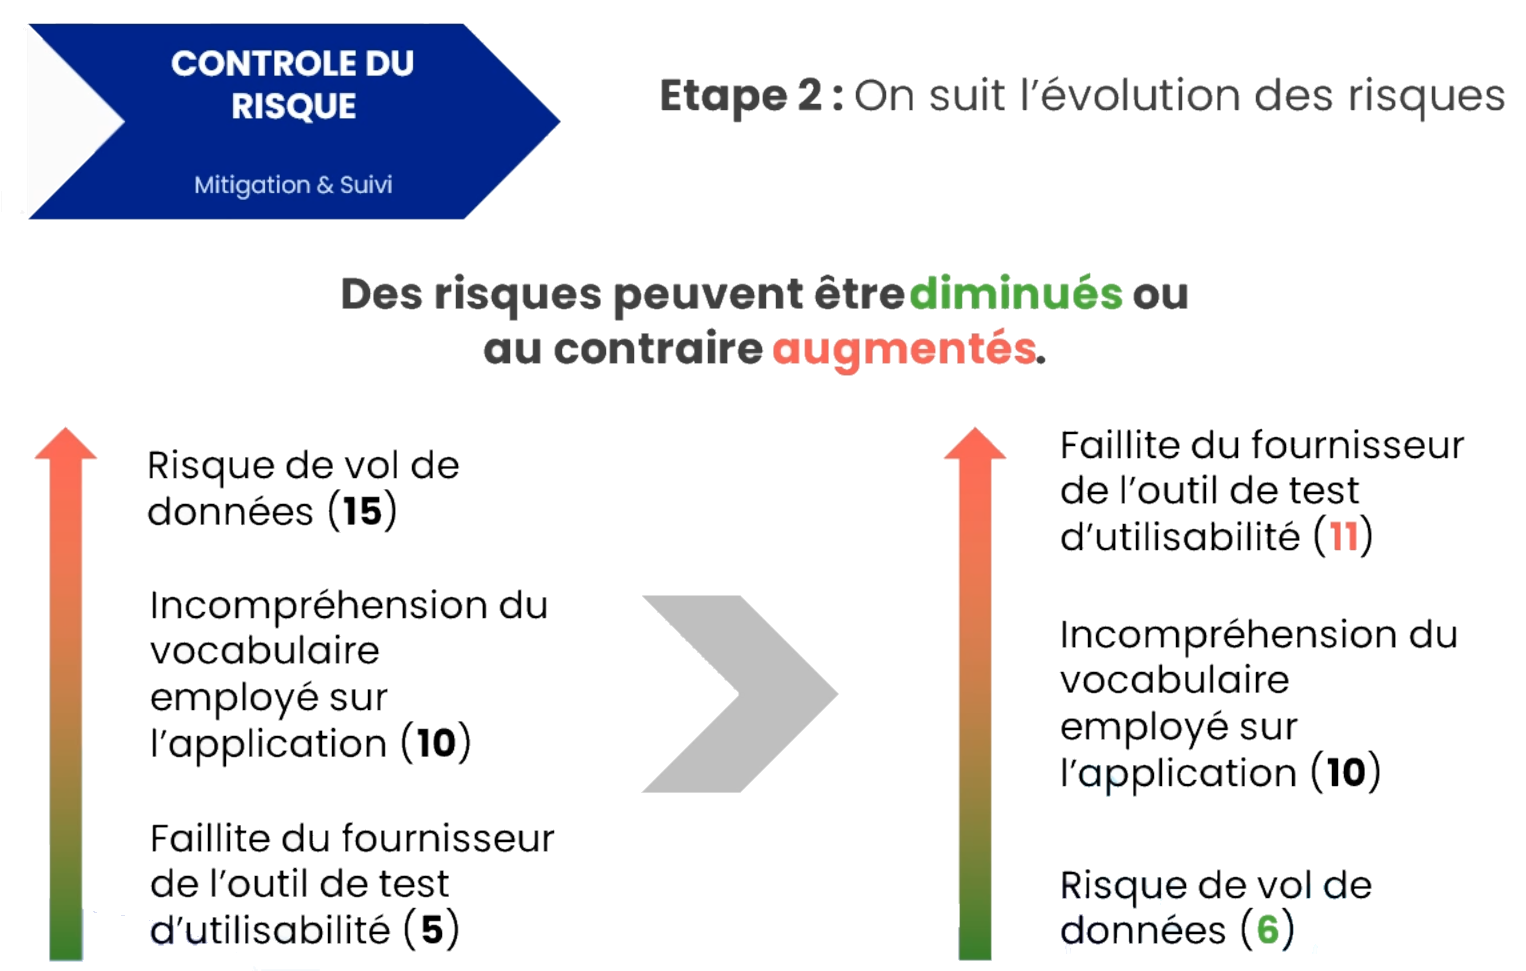
\includegraphics[width=0.9\textwidth]{images/controle_risque_02.png}
        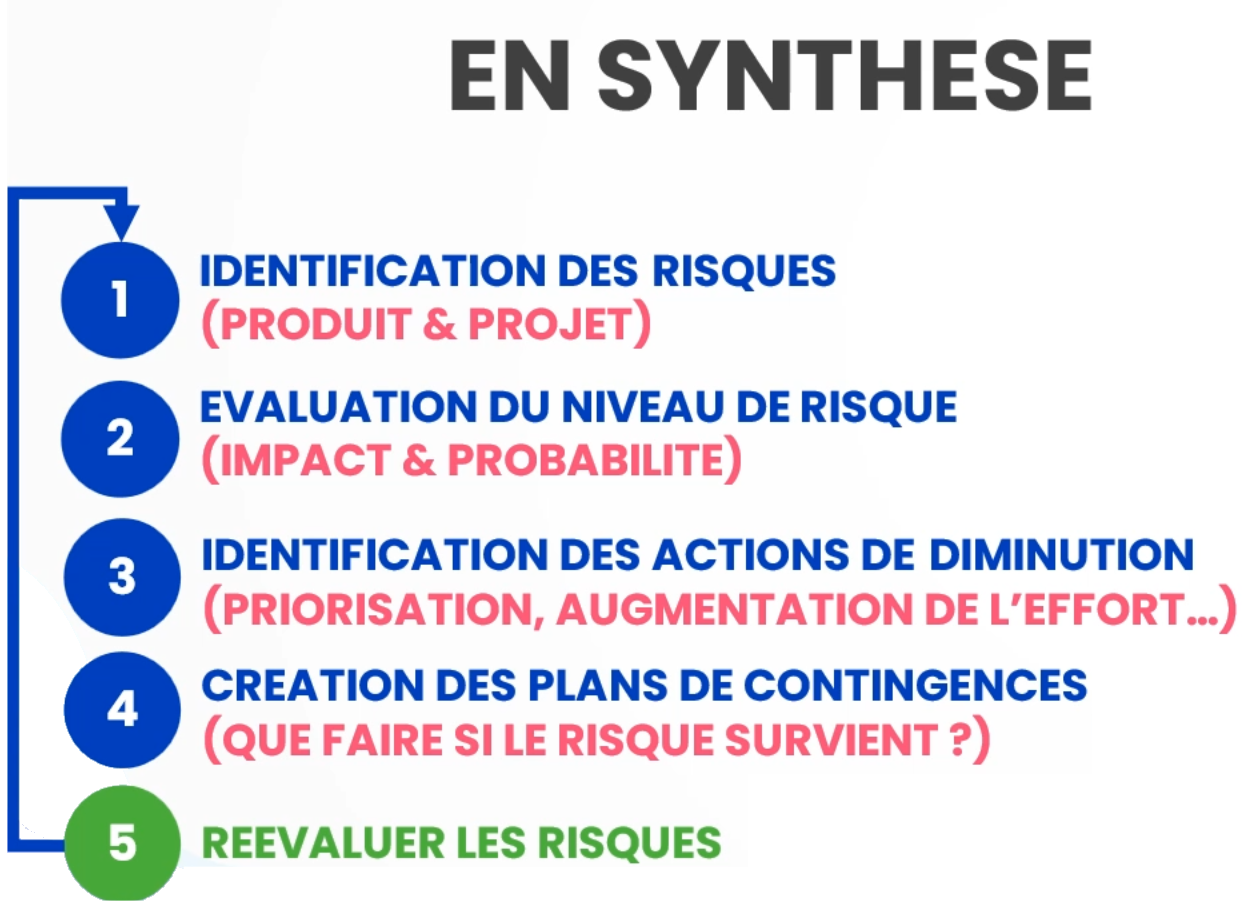
\includegraphics[width=0.9\textwidth]{images/controle_risque_03.png}
    \end{center}
    
	\subsection{Les métriques}

    \begin{center}
        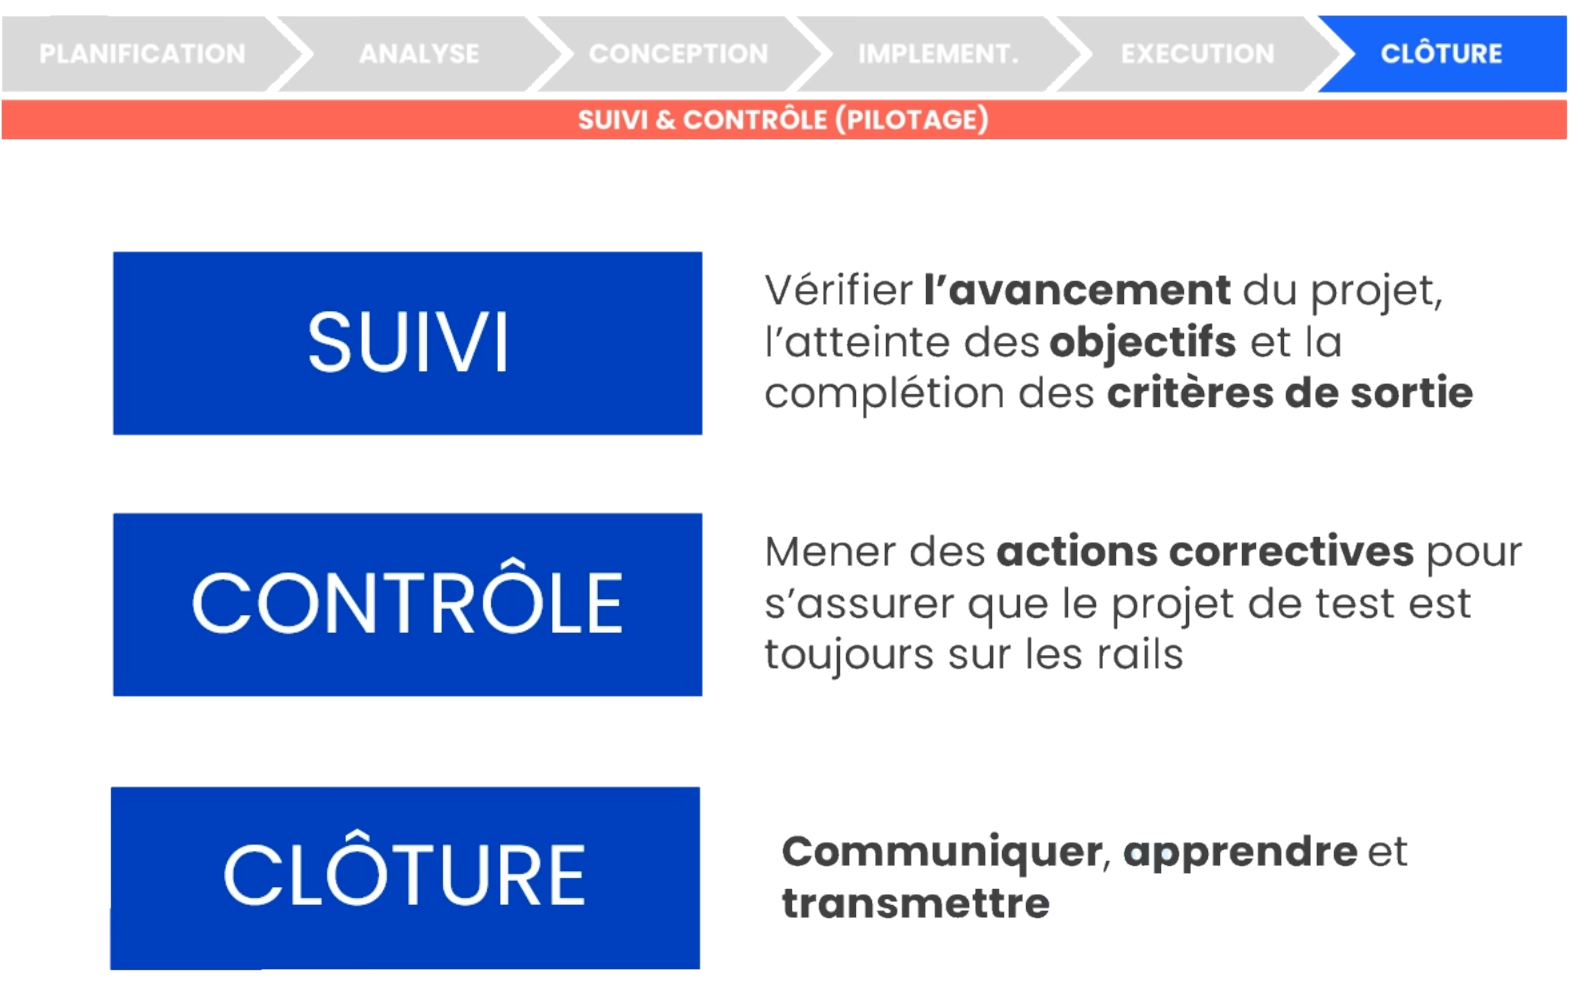
\includegraphics[width=0.9\textwidth]{images/metriques_01.png}
        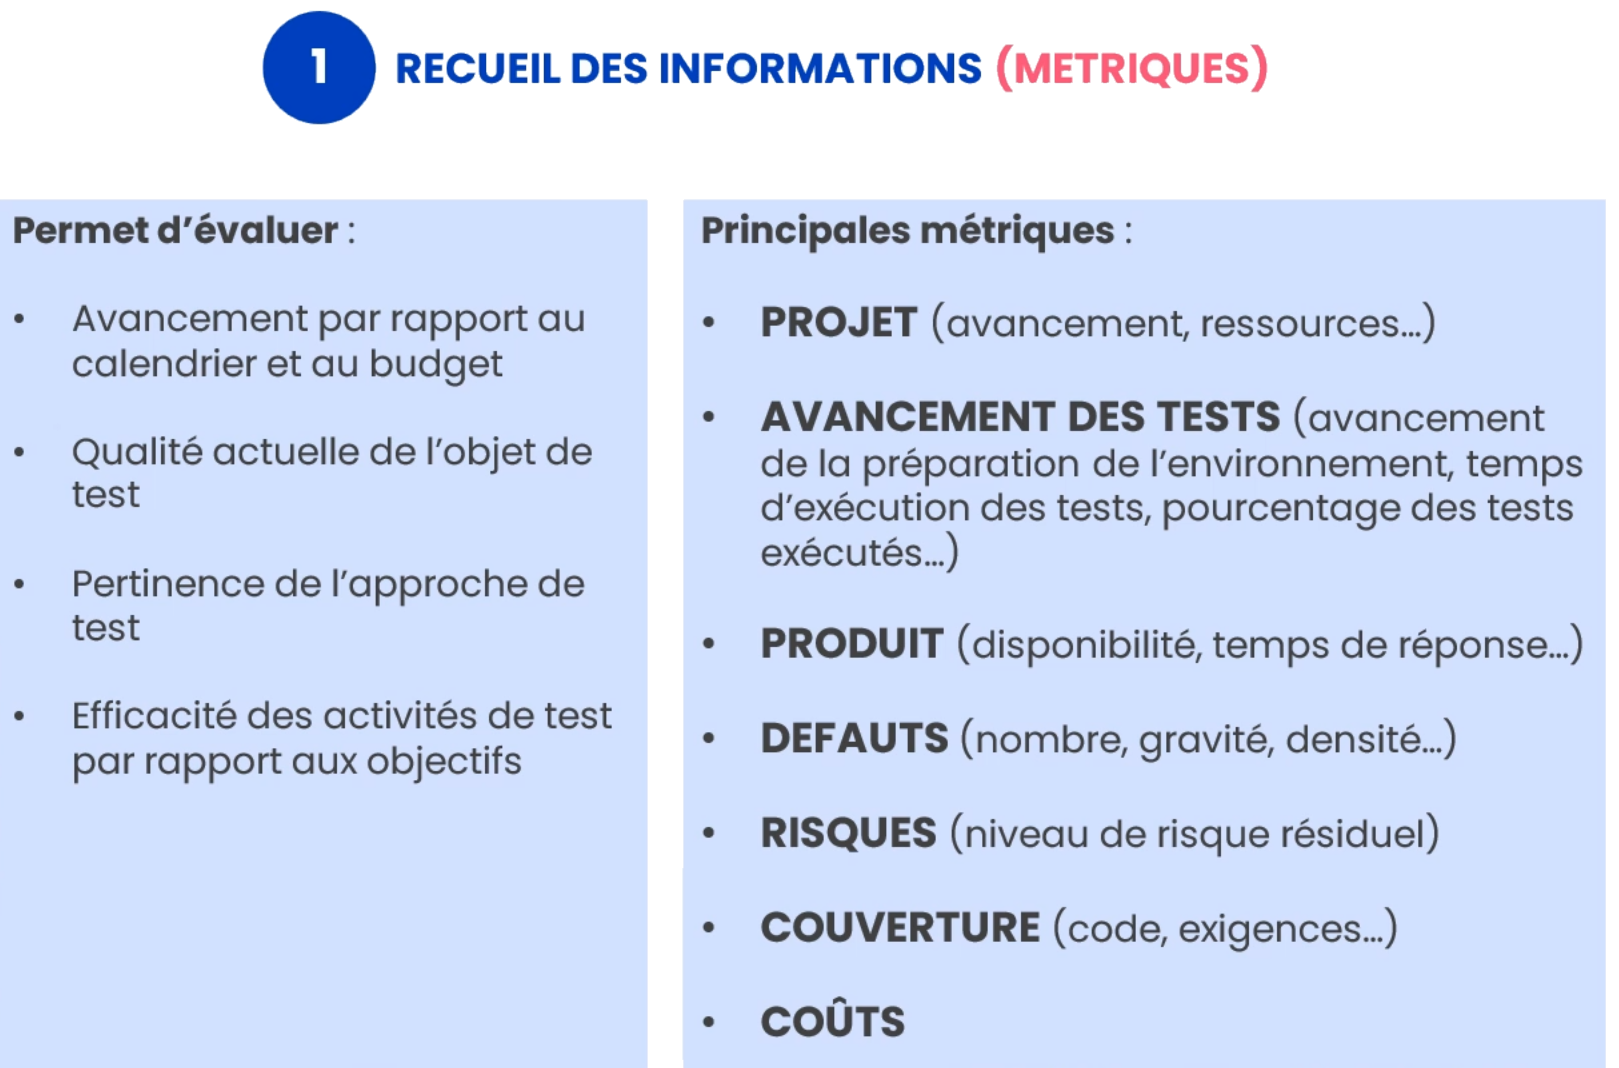
\includegraphics[width=0.9\textwidth]{images/metriques_02.png}
    \end{center}
    
	\subsection{Le rapport}

    \begin{center}
        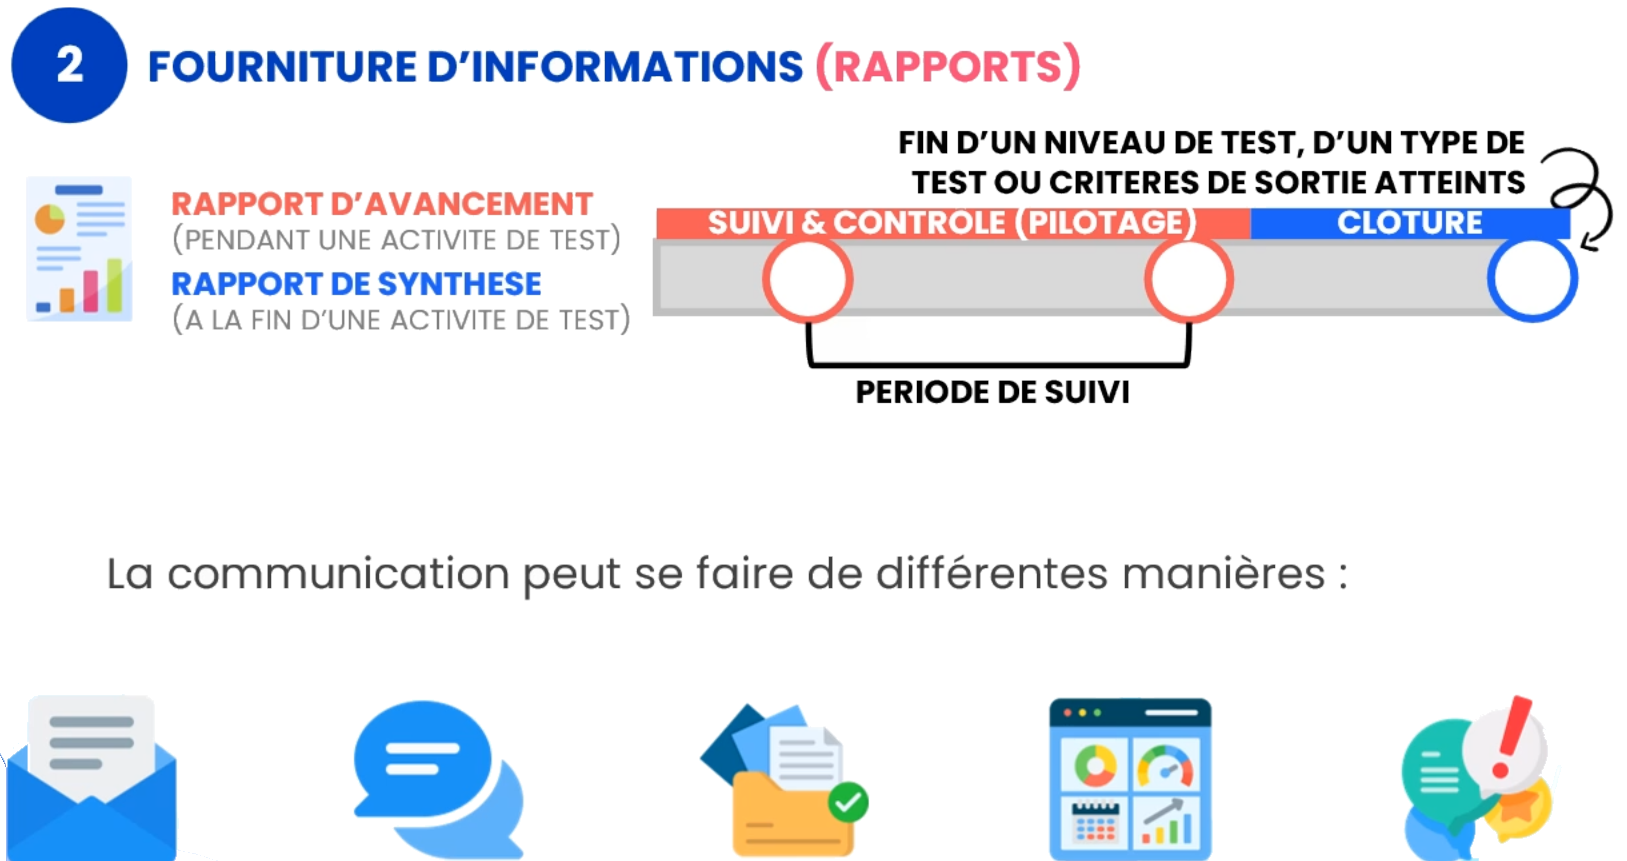
\includegraphics[width=0.9\textwidth]{images/rapports_01.png}
        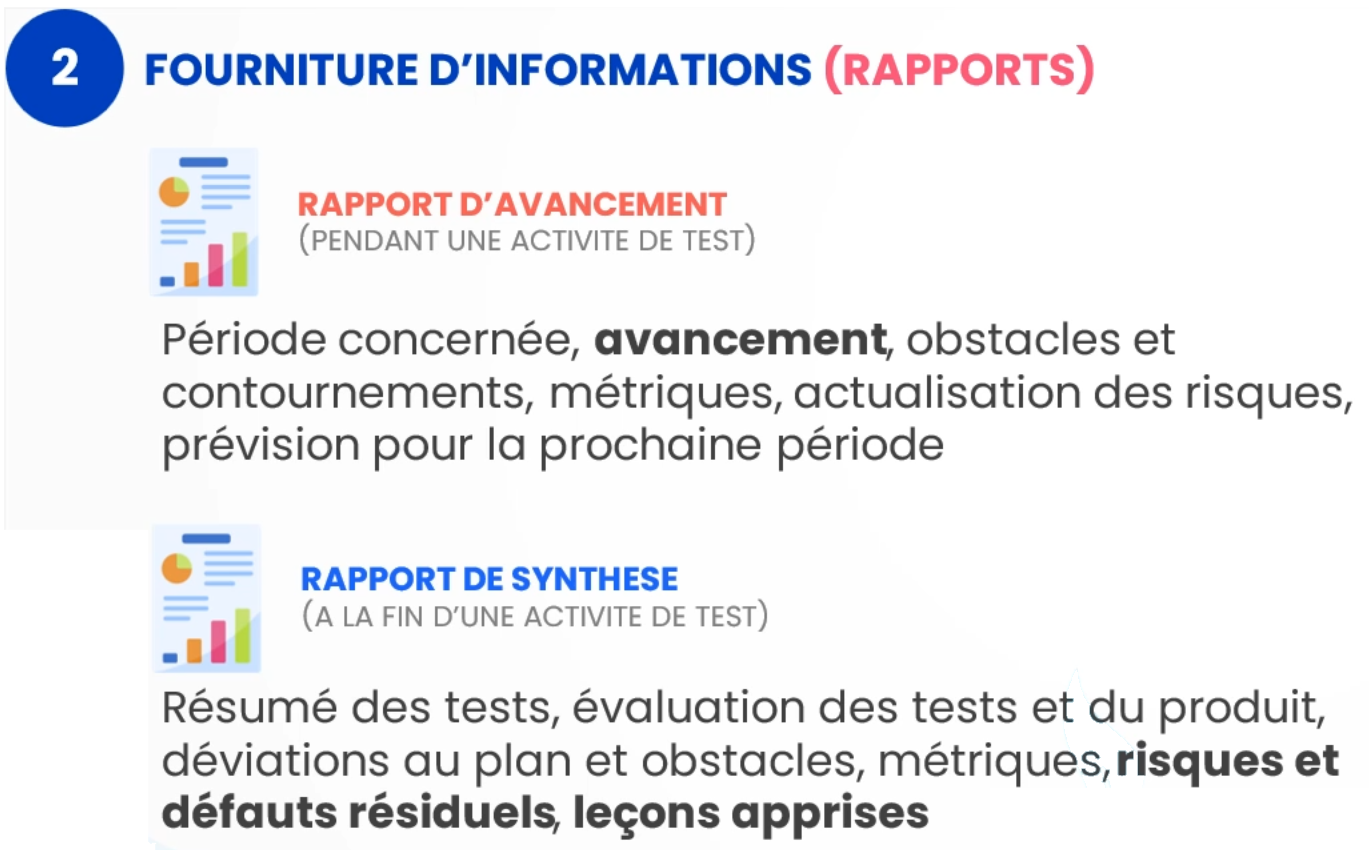
\includegraphics[width=0.9\textwidth]{images/rapports_02.png}
    \end{center}

	\subsection{La gestion de configuration}

    \begin{center}
        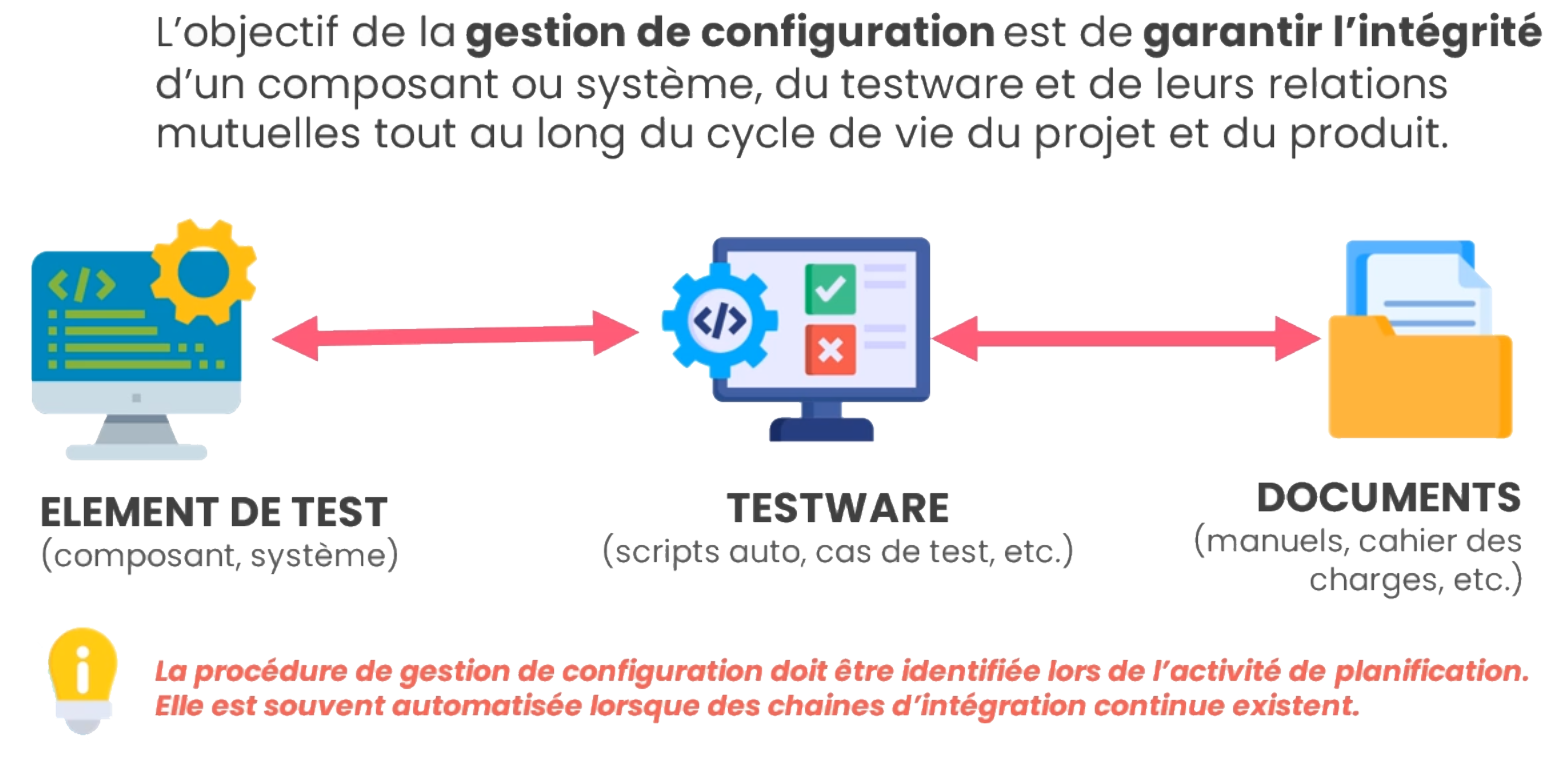
\includegraphics[width=0.9\textwidth]{images/gestion_de_conf.png}
    \end{center}
    
	\subsection{La gestion des défauts}

    \begin{center}
        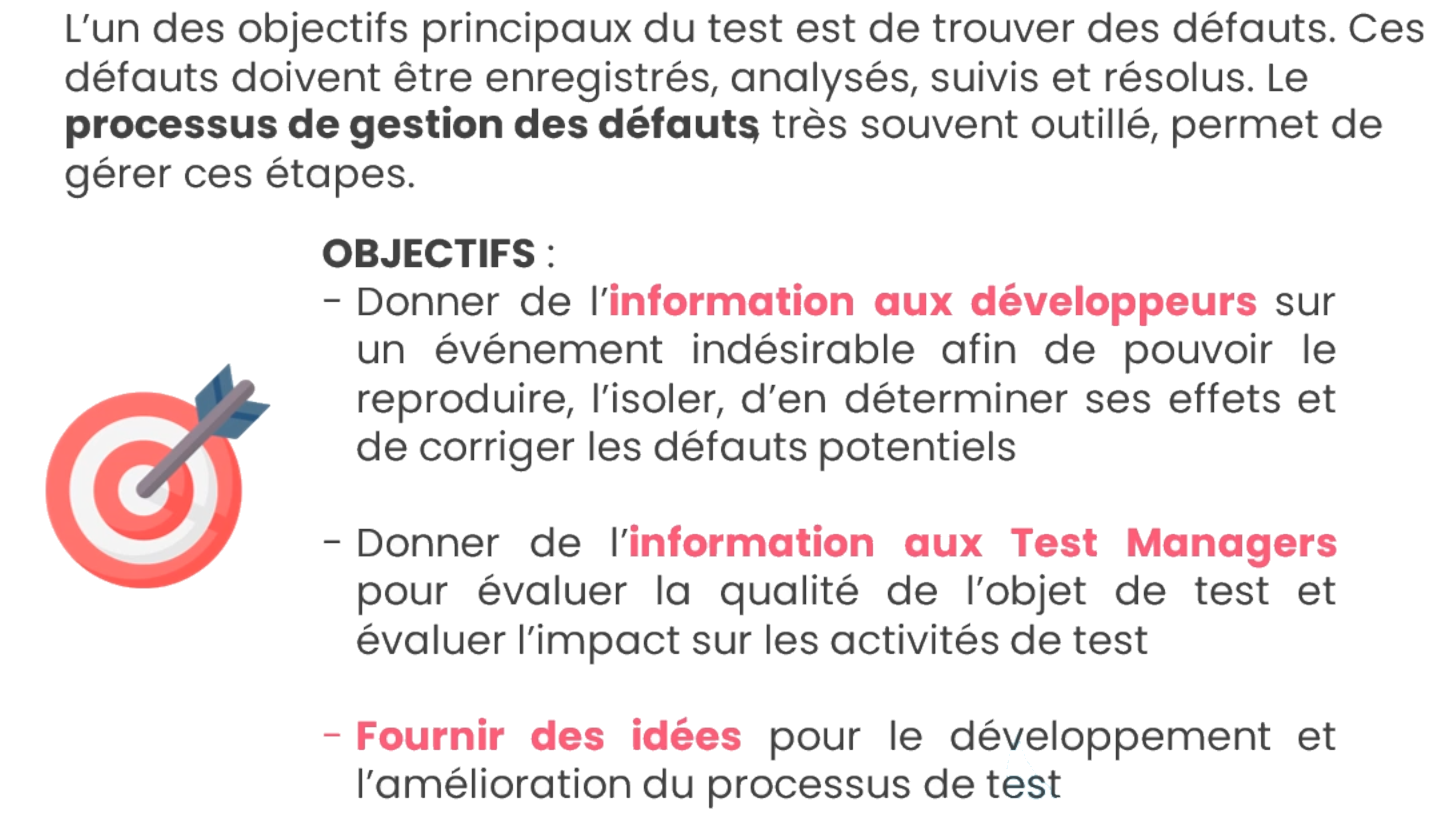
\includegraphics[width=0.9\textwidth]{images/gestion_defauts_01.png}
        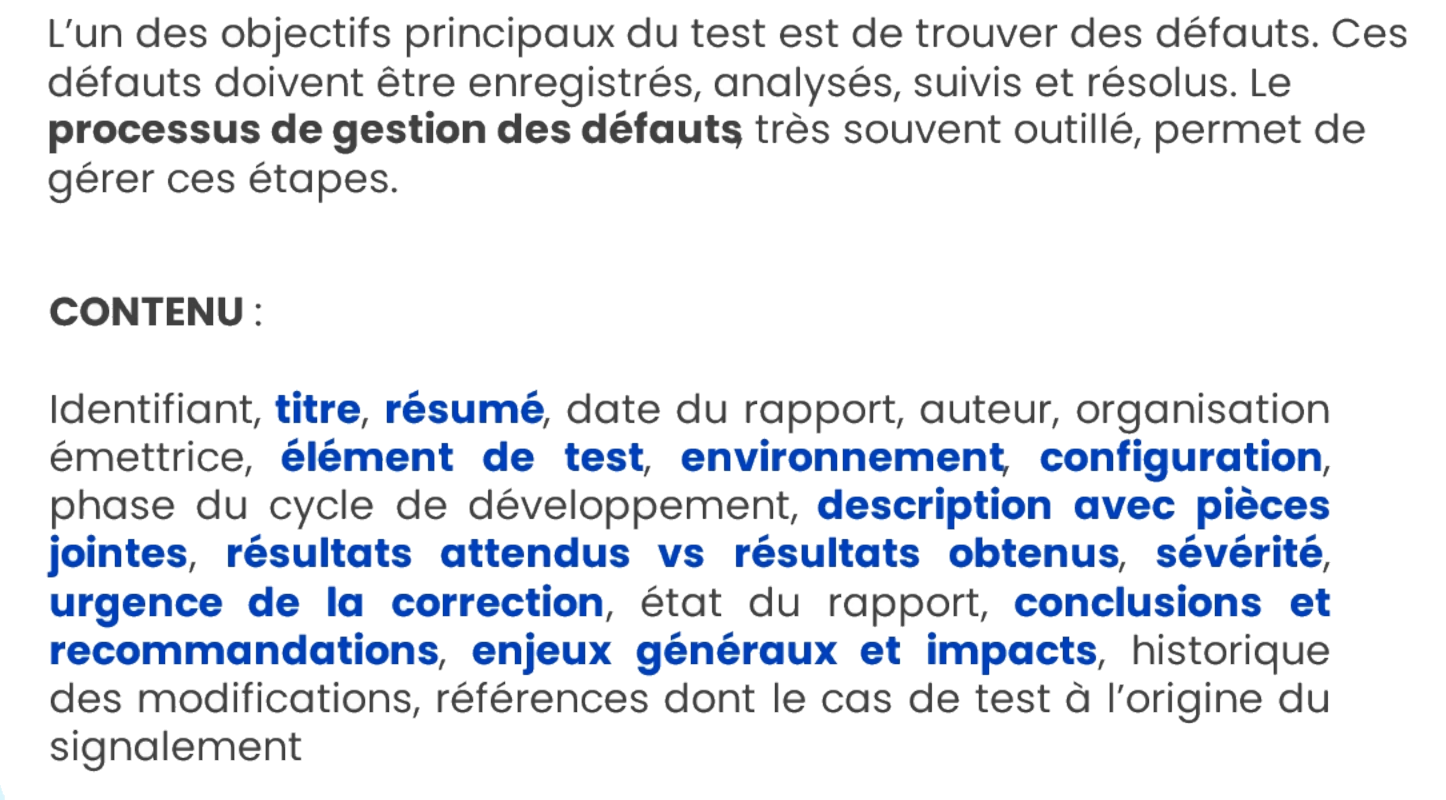
\includegraphics[width=0.9\textwidth]{images/gestion_defauts_02.png}
    \end{center}


\pagebreak
\section{OUTILS DE TEST}

	\subsection{Les types d'outils}

    \begin{center}
        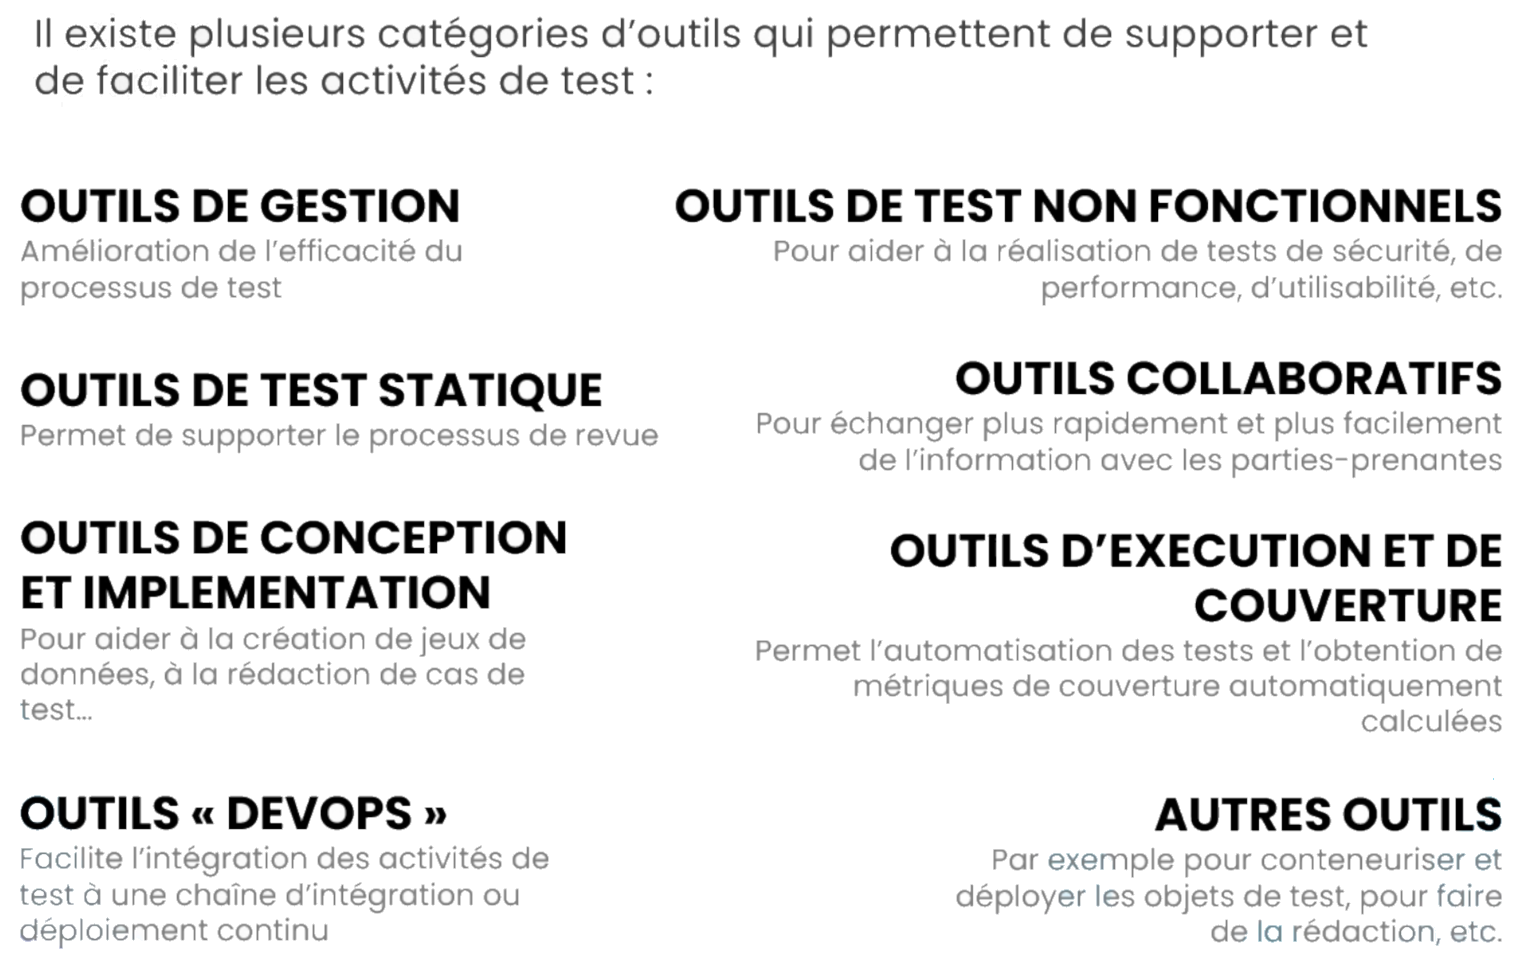
\includegraphics[width=0.9\textwidth]{images/outils.png}
    \end{center}
    
	\subsection{Introduction d'un outil}

    \begin{center}
        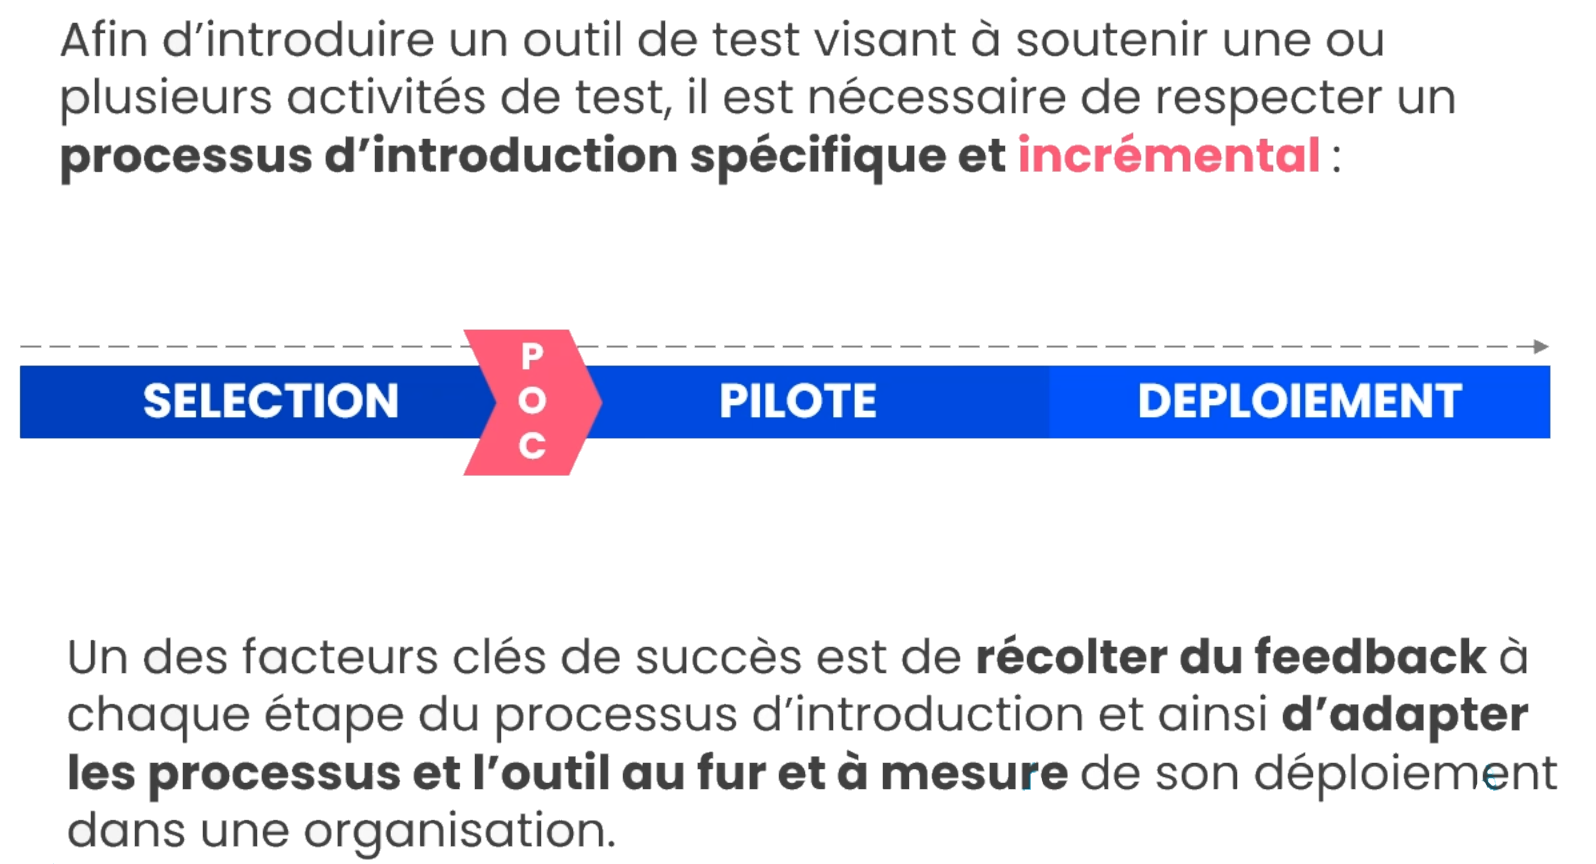
\includegraphics[width=0.9\textwidth]{images/intro_outils_01.png}
        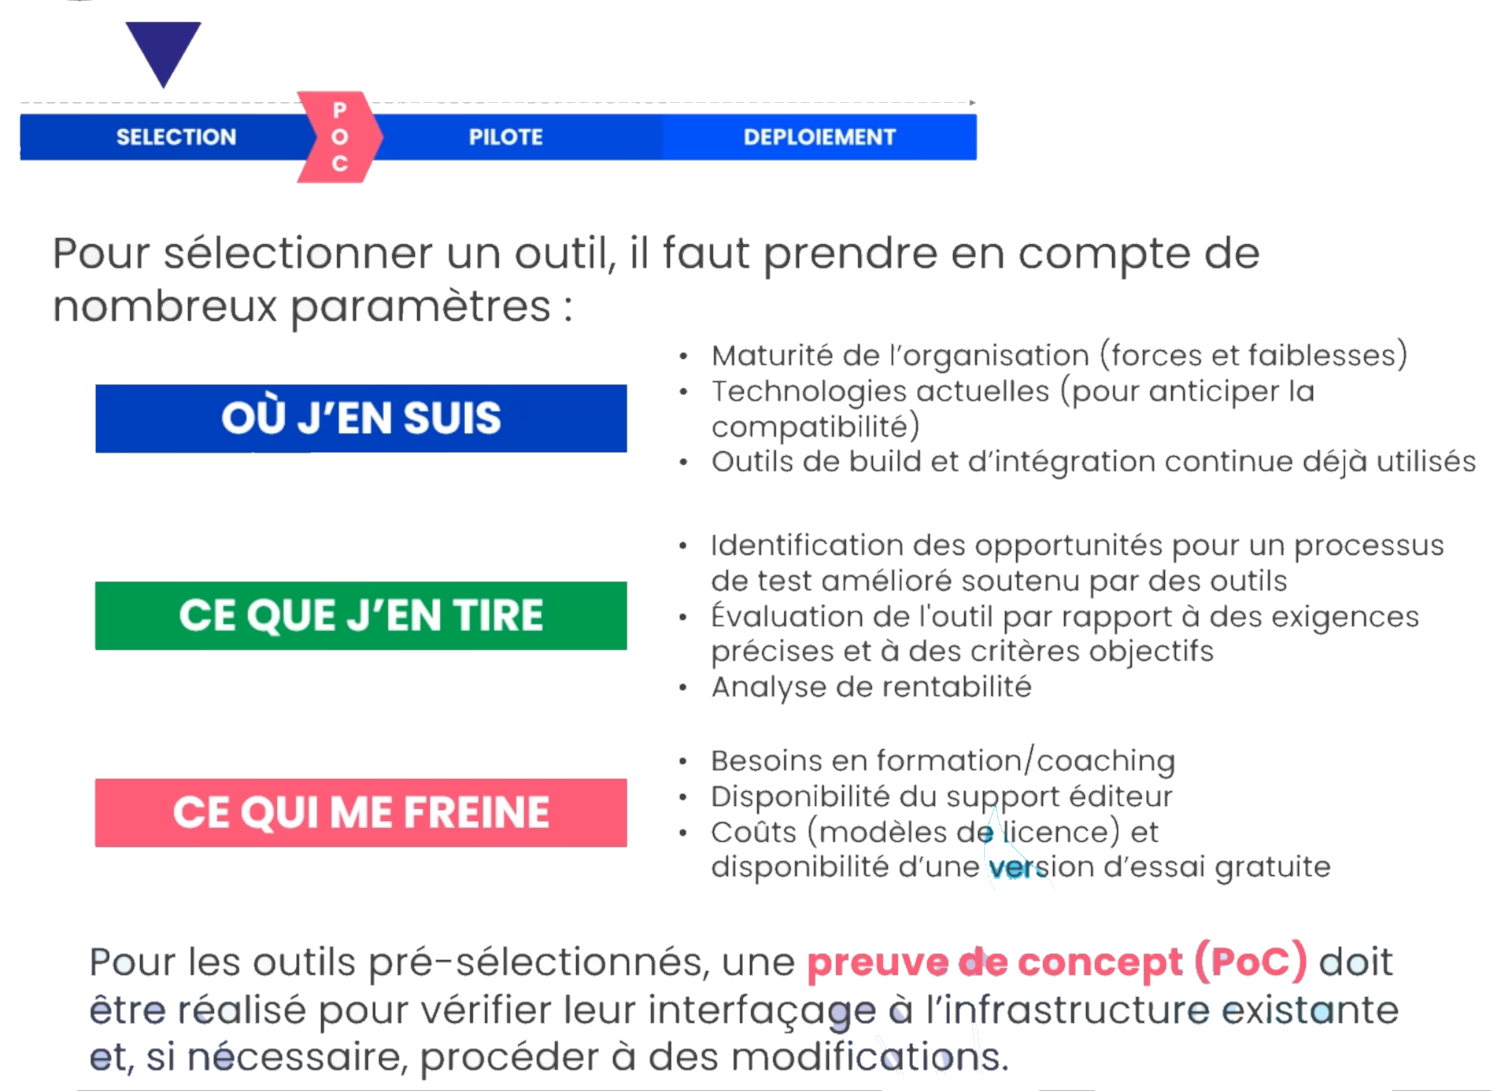
\includegraphics[width=0.9\textwidth]{images/intro_outils_02.png}
        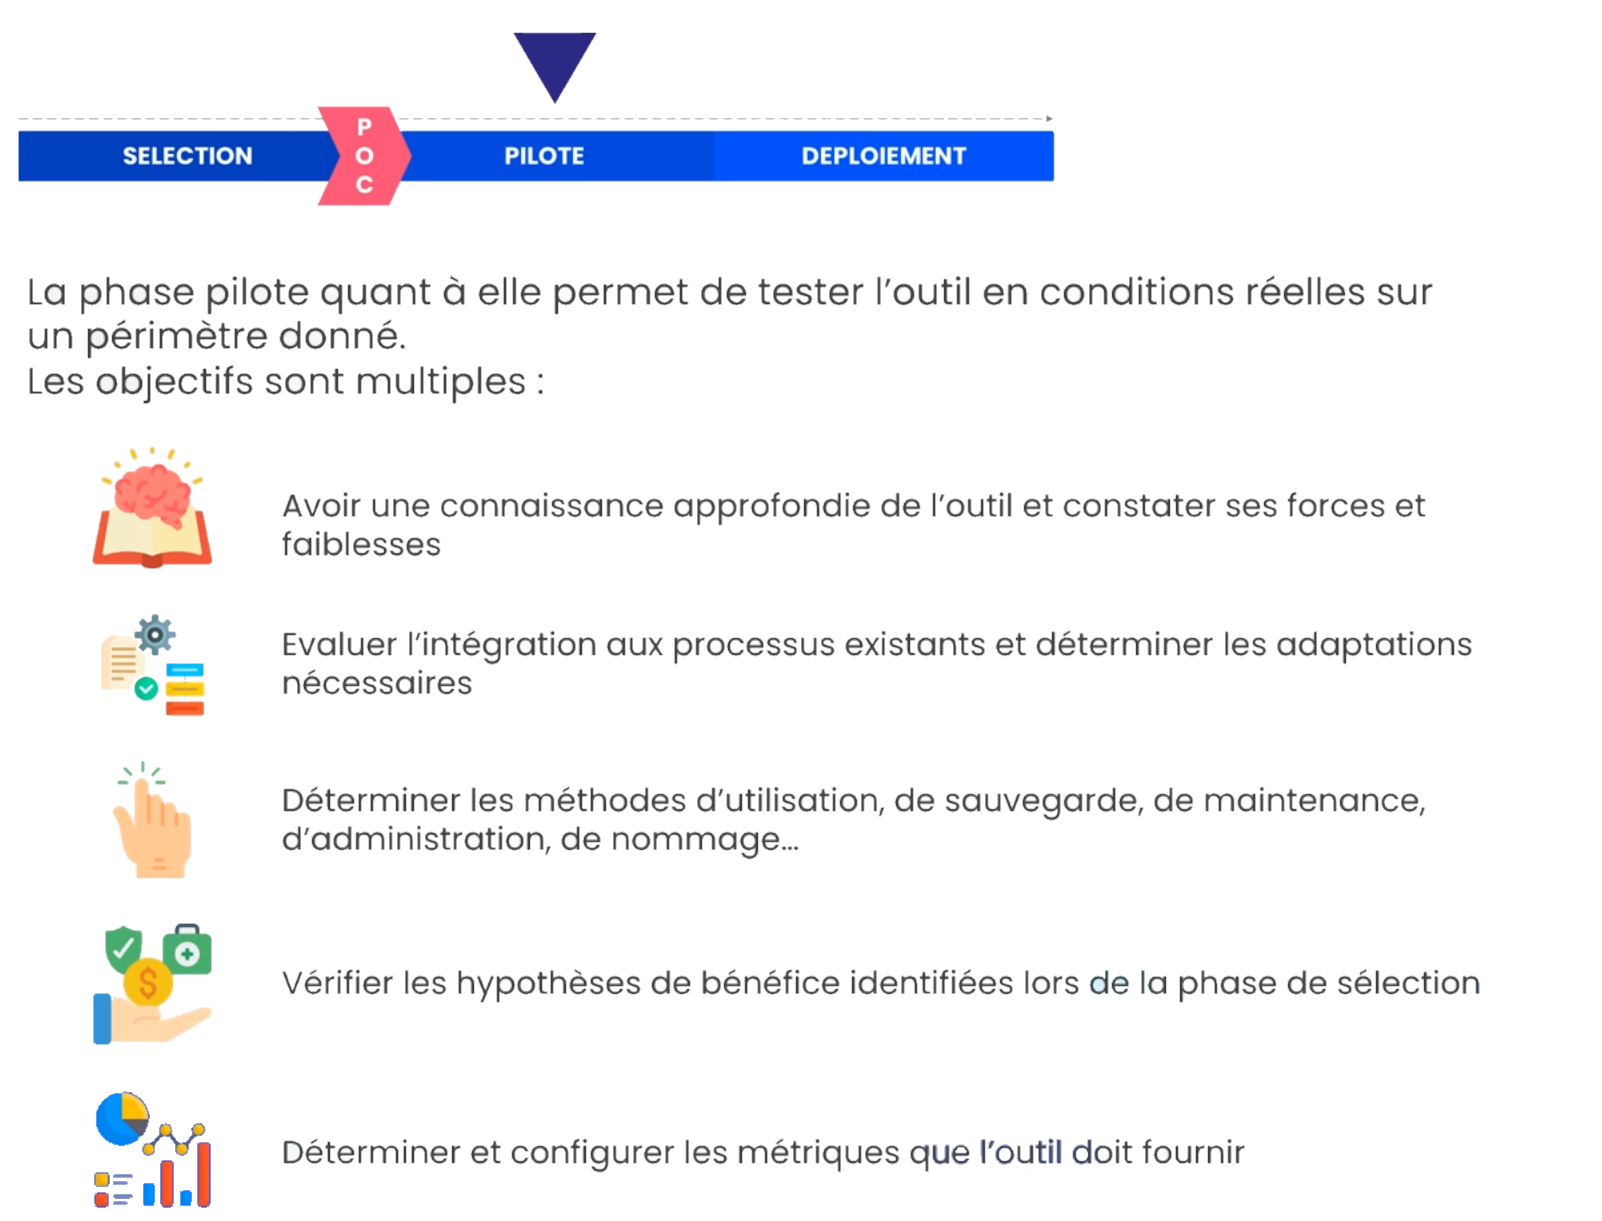
\includegraphics[width=0.9\textwidth]{images/intro_outils_03.png}
        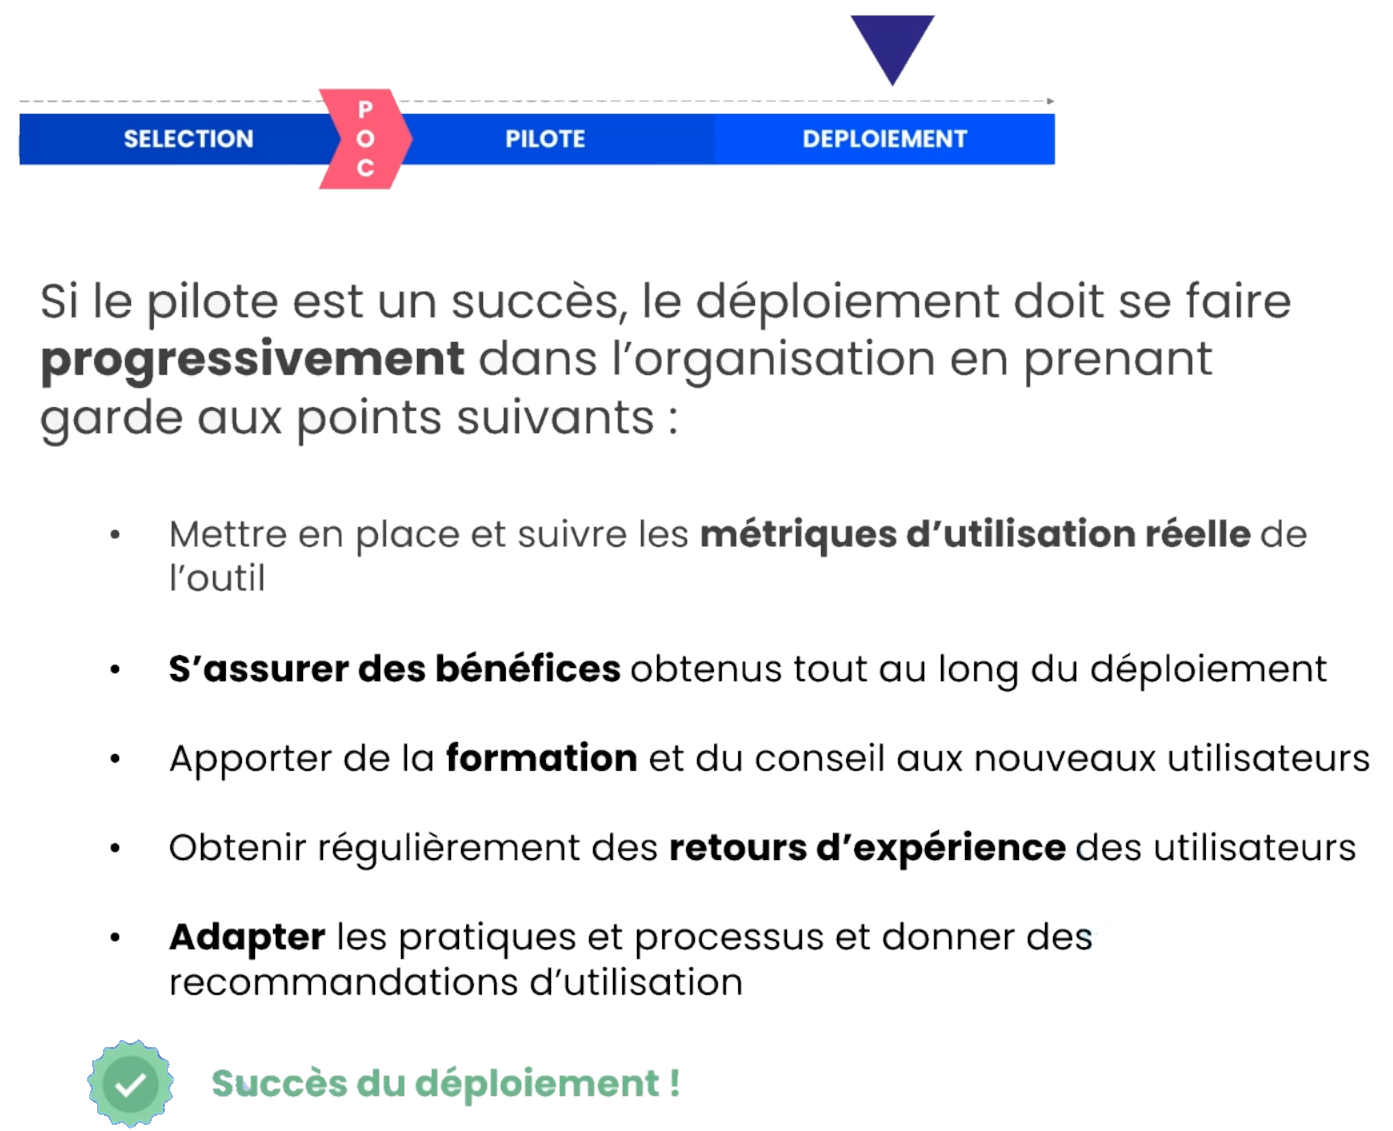
\includegraphics[width=0.9\textwidth]{images/intro_outils_04.png}
    \end{center}
    
	\subsection{L'automatisation}

    \begin{center}
        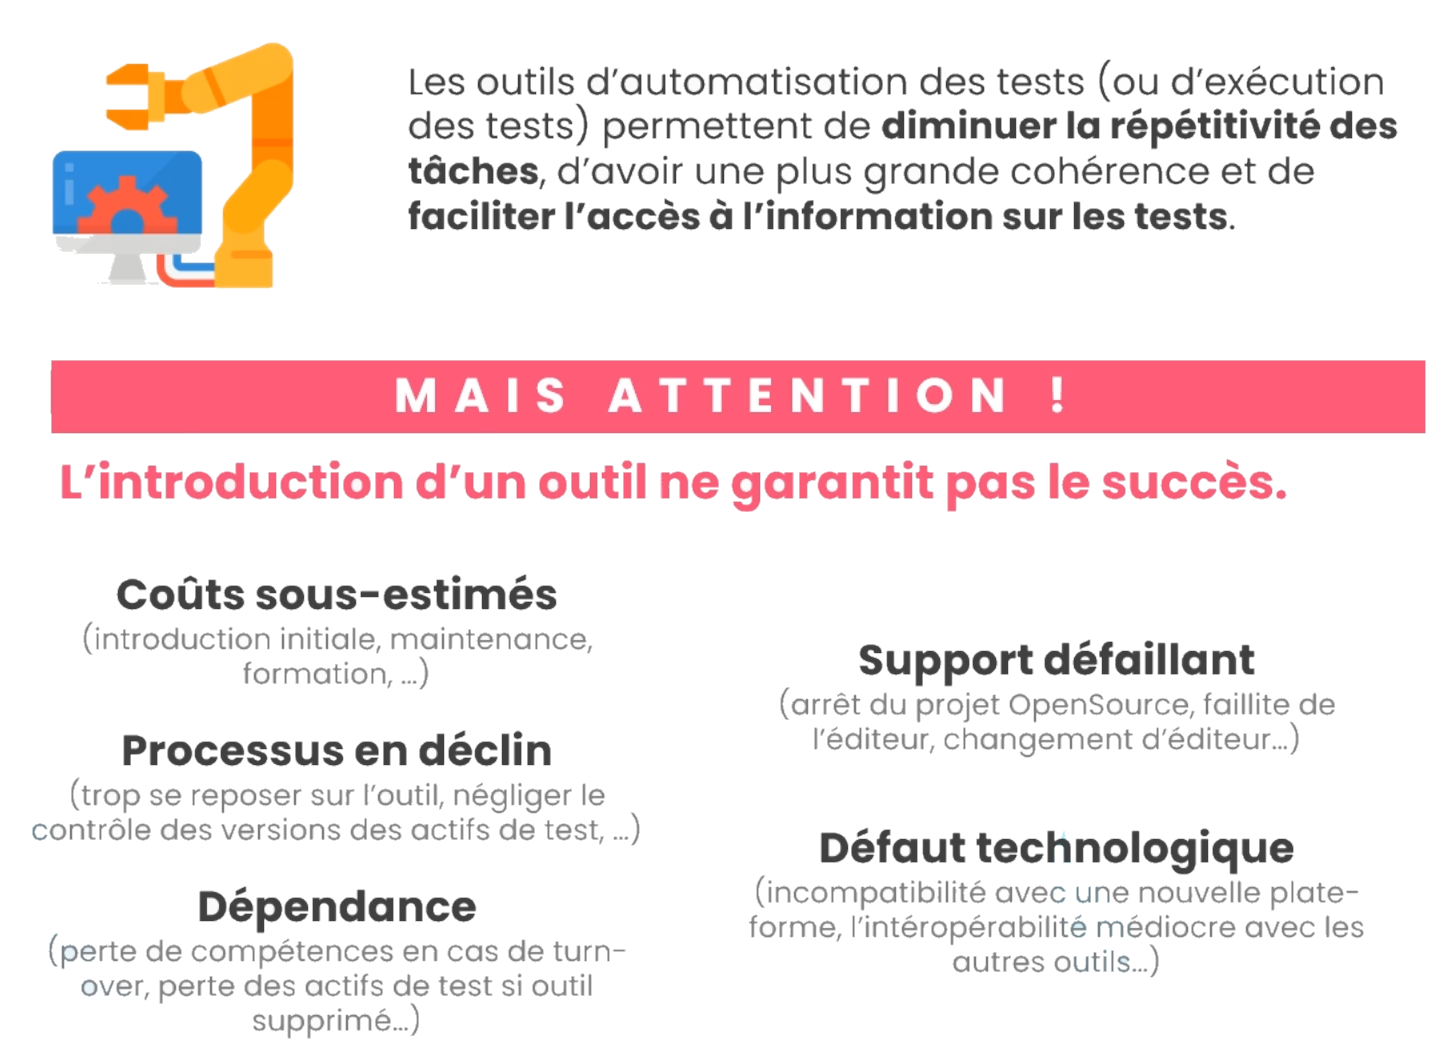
\includegraphics[width=0.9\textwidth]{images/automatisation_01.png}
        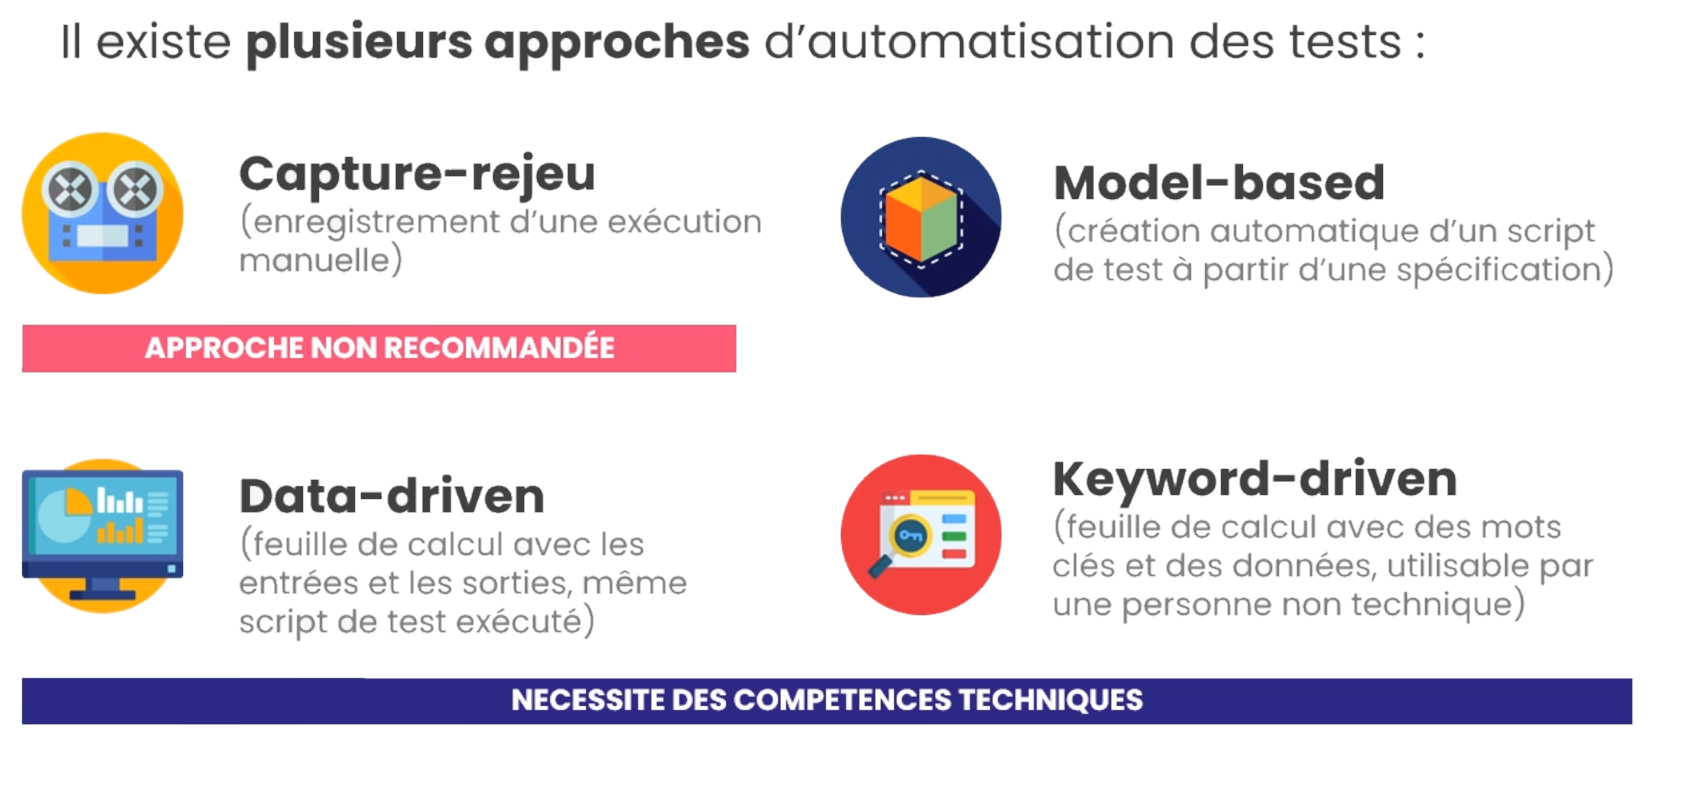
\includegraphics[width=0.9\textwidth]{images/automatisation_02.png}
    \end{center}
    
	\subsection{La gestion de test}

    Squash
    
	% \subsection{Outils Exemple Et Automatisation}
	% \subsection{Outils Résumé}


\printbibliography

\end{document}


% https://tex.stackexchange.com/questions/66820/how-to-create-highlight-boxes-in-latex
% https://tex.stackexchange.com/questions/75667/change-colour-on-chapter-section-headings-lyx
% https://tex.stackexchange.com/questions/430542/a-fancy-and-beautiful-type-of-enumerate
% https://tex.stackexchange.com/questions/282044/how-to-fill-a-circle-node
% https://fr.overleaf.com/learn/latex/Lists
% https://tex.stackexchange.com/questions/312574/colorbox-does-not-linebreak
% https://tex.stackexchange.com/questions/141569/highlight-textcolor-and-boldface-simultaneously
